%%%%%%%%%%%%%%%%%%%%%%%%%%%%%%%%%%%%%%%%%%%%%%%%%%%%%%%%%
%%   $RCSfile: hpsg-include.tex,v $
%%      $Date: 2014/09/09 12:19:27 $
%%     Author: Stefan Mueller (FU Berlin)
%%    Purpose: 
%%   Language: LaTeX
%%%%%%%%%%%%%%%%%%%%%%%%%%%%%%%%%%%%%%%%%%%%%%%%%%%%%%%%%

%\hypersetup{bookmarksopenlevel=0}






%\renewcommand{\centerfit}[1]{}





\begin{document} 

\include{title-toc}


 %% -*- coding:utf-8 -*-
\chapter{Vorwort}

Dieses Buch verfolgt zwei Ziele: erstens die vergleichende Analyse der wichtigsten syntaktischen Eigenschaften der
\ili{germanisch}en Sprachen und zweitens die Einführung eines bestimmten Formats für die Beschreibung und
den Vergleich von Sprachen. Der Rahmen, in dem die Analysen formuliert werden, heißt \emph{HPSG
  light}. Er basiert auf der Head-Driven Phrase Structure Grammar (HPSG) \citep{ps,ps2,HPSGHandbook} in der speziellen Version, die ausführlich in
\citew{MuellerLehrbuch3} beschrieben wird. HPSG light enthält allerdings keine komplizierten Merkmal"=Wert"=Matrizen
(AVMs). Sofern überhaupt AVMs verwendet werden, sind sie auf das Minimum reduziert und enthalten nur eine kleine Menge
von Merkmalen wie \argst für die Argumentstruktur, \comps für die Komplemente und \spr für den Spezifikator. Alle
übrigen Aspekte der Analysen werden in syntaktischen Bäumen dargestellt, die leichter zu lesen sind. Die Idee
hinter der Einführung von HPSG light besteht darin, ein Werkzeug für Linguistinnen und Linguisten bereitzustellen, die ein
Phänomen detaillierter beschreiben wollen, ohne sich dabei zwangsläufig mit allen
technischen Einzelheiten befassen zu müssen. Der Grad der Formalisierung entspricht dem, was in der Government"=and"=Binding"=Theorie,
im Minimalismus und in den weniger formalen Varianten der Konstruktionsgrammatik üblich ist. Was die eine formale Version
der Konstruktionsgrammatik betrifft, die eine Variante der HPSG ist, nämlich die Sign-Based Construction Grammar (SBCG, \citealp{Sag2012a}), so kann HPSG
light auch als eine Light"=Version von SBCG betrachtet werden, da die Unterschiede in den
abgekürzten Darstellungen und Bäumen, die in diesem Buch verwendet werden, vernachlässigt werden. Die hier vorgestellte Arbeit unterscheidet sich
von nicht"=formaler Arbeit in GB/Minimalismus und Konstruktionsgrammatik in einem wichtigen Punkt: Sie wird
durch implementierte Grammatiken gestützt, die die vollständige Version der HPSG einschließlich einer semantischen Analyse im
Rahmen der Minimal Recursion Semantics (MRS, \citew*{CFPS2005a}) verwenden. Die detaillierten Analysen werden in
Konferenzbänden, Zeitschriftenartikeln und Büchern beschrieben, und die Leserin bzw.\ der Leser ist eingeladen, diese
Quellen zu konsultieren, falls Interesse an den Details besteht. Die implementierten Grammatiken werden
mit der virtuellen Maschine Grammix \citep{MuellerGrammix} verteilt und können von der Webseite des Autors
heruntergeladen werden.\footnote{
\url{https://hpsg.hu-berlin.de/Software/Grammix/}, \today.} Grammix enthält die Grammatiken für
\ili{Deutsch}\footnote{
\url{https://hpsg.hu-berlin.de/Fragments/Berligram/}, \today. Die \ili{deutsch}e Grammatik ist in
\citew{MuellerLehrbuch,MuellerGS} und \citew{MOe2011a,MOe2013a} dokumentiert.
},
\ili{Dänisch}\footnote{
\url{https://hpsg.hu-berlin.de/Fragments/Danish/}, \today. Die \ili{dänisch}e Grammatik ist in
\citew{MOeDanish,MOe2013a,MOe2011a,MOe2013b} dokumentiert.
}, \ili{Englisch}\footnote{
\url{https://hpsg.hu-berlin.de/Fragments/English/}, \today. Die \ili{englisch}e Grammatik ist kleiner als die
\ili{deutsch}e und die \ili{dänisch}e Grammatik. Sie ist ein Proof of Concept einer lexikalistischen Analyse von Passiv, Benefaktiv\-
konstruktionen und Resultativkonstruktionen. Siehe \citew{MuellerLFGphrasal} und \citew{MOe2013a} für Details.
} und \ili{Jiddisch}\footnote{
\url{https://hpsg.hu-berlin.de/Fragments/Yiddish/}, \today. Die \ili{jiddisch}e Grammatik basiert auf
\citew{MOe2011a} und unveröffentlichter Arbeit von Jong-Bok Kim, Alain Kihm und mir zur
Prädikatstopikalisierung im \ili{Koreanisch}en und \ili{Jiddisch}en \citep*{MKK2019a}.
} die im Projekt CoreGram \citep{MuellerCoreGram} entwickelt wurden. Die jeweiligen Webseiten der Grammatiken enthalten eine Liste von Testsätzen,
die von den Grammatiken akzeptiert oder zurückgewiesen werden. Die Leserinnen und Leser sind eingeladen, diese
Sätze in das TRALE-System \citep{DKMM2004a-u,Penn2004a-u} einzugeben, das mit Grammix geliefert wird, und die vollständigen AVMs zu inspizieren.

Das Buch beginnt mit zwei einführenden Kapiteln: Das erste Kapitel stellt die \ili{germanisch}en Sprachen vor
und liefert grundlegende Fakten wie die Zahl der Sprecher, die Gebiete, in denen sie gesprochen werden, und einige historische
Fakten. Das zweite Kapitel behandelt die Phänomene, die im Rest des Buches behandelt werden, \eg Scrambling,
die Stellung von Adverbialen, Passiv, Satztypen und Fernabhängigkeiten. Das dritte Kapitel ist eine
Einführung in Phrasenstrukturgrammatiken, die seit \citegen{Chomsky57a} Formalisierung strukturalistischer Ideen
\citep{Bloomfield33a-u} die Grundlage fast aller Theorien bilden. Kapitel~\ref{chap-psg-xbar} führt nicht nur Phrasenstrukturgrammatiken ein,
sondern auch Grammatiken, die Abstraktionen über Phrasenstrukturregeln verwenden und letztlich zu sehr
abstrakten Grammatiken des auch aus der \xbart
\citep{Jackendoff77a} bekannten Typs führen. Kapitel~\ref{chap-valence} erklärt, wie das Konzept der Valenz
mit abstrakten Phrasenstrukturregeln kombiniert wird, um sicherzustellen, dass die richtige Anzahl und die richtige Art von
Elementen mit einem bestimmten Wort kombiniert wird. Zum Beispiel braucht ein Wort wie \emph{lachen} ein Subjekt und
ein Wort wie \emph{lesen} ein Subjekt und ein Objekt. Das muss irgendwo in einer
Grammatik repräsentiert werden, und Kapitel~\ref{chap-valence} erklärt, wie das in HPSG (light) gemacht wird. Die grundlegenden Unterschiede
in den Analysen von SVO- und SOV-Sprachen werden erläutert. Dieses Kapitel
erklärt außerdem, wie sich die verschiedenen Abfolgen von Subjekt und Objekten in einer Sprache wie dem \ili{Deutsch}en erklären lassen
(das sogenannte \emph{Scrambling}) und wie man die verschiedenen Stellungsmöglichkeiten in Sprachen wie dem \ili{Englisch}en
und den nord\ili{germanisch}en Sprachen einerseits und dem \ili{Deutsch}en, \ili{Niederländisch}en und \ili{Afrikaans} andererseits erfassen kann. Verbalkomplexe werden in Kapitel~\ref{chap-verbal-complex} behandelt, die Verberststellung (zur Fragebildung verwendet) und die Verbzweitstellung (für Aussagen) werden
in Kapitel~\ref{chap-verb-position} erläutert. Passiv und Kasuszuweisung im Allgemeinen werden in
Kapitel~\ref{chap-case} behandelt. Die \ili{germanisch}en Sprachen sind hier besonders interessant, da das \ili{Isländisch}e
zu dieser Sprachgruppe gehört und für seine quirky subjects bekannt ist (Subjekte im Genitiv, Dativ oder
Akkusativ, \citealp{ZMT85a}). Kapitel~\ref{chap-expletives} behandelt Expletivpronomen und wie sie
in den \ili{germanisch}en Sprachen verwendet werden, um Satztypen zu markieren. Zum Beispiel werden Expletiva im
\ili{Deutsch}en in Hauptsätzen verwendet, um die Anfangsposition zu füllen, sodass der Satz eine Aussage ist. Das \ili{Dänisch}e verwendet
Expletiva in eingebetteten Sätzen mit Subjekten als Interrogativelementen. Auch hier beeinflussen die Unterschiede in den
allgemeinen grammatischen Eigenschaften die Grammatik in anderen Bereichen, etwa bei der Stellung von Expletiva.

% The final chapter, Chapter~\ref{chap-HPSG-light}, is for advanced readers. It tries to relate the simplified version
% of HPSG that was used throughout the earlier chapters to HPSG as it is used in full-fledged HPSG publications.

Das letzte Kapitel, Kapitel~\ref{chap-outlook}, fasst kurz zusammen, was im Buch geschehen ist, und
verweist die interessierte Leserin bzw.\ den interessierten Leser auf einige weiterführende Literatur zur HPSG.

\ili{Deutsch}sprachige Folien, die für den von mir mit diesem Buch gehaltenen Kurs entwickelt wurden, sind auf GitHub verfügbar.\footnote{
\url{https://github.com/stefan11/germanic-syntax-slides}, 2021-09-14.
}
\ili{Deutsch}sprachige Vorlesungen zu den Kapiteln finden sich außerdem auf YouTube.\footnote{
\url{https://www.youtube.com/playlist?list=PLXwGGsuPxWRp4AB2LsWH6LKc0II7uc6tg}
}

\section*{Zur Art der Veröffentlichung dieses Buches}

Lehrkräfte an Schulen und an vielen Universitäten werden vom Staat bezahlt, das heißt von der Öffentlichkeit (von Ihnen). Zu
ihren Aufgaben gehört die Erstellung von Lehrmaterial. Es gibt überhaupt keinen Grund, das
Lehrmaterial profit"=orientierten Verlagen zu überlassen. Im Gegenteil, Lehrmaterial sollte offen
und an die Bedürfnisse der Lehrenden anpassbar sein, die es verwenden wollen.

Eine Studie des American Enterprise Institute zeigt, dass der Preis von Hochschulbüchern von 1978 bis 2012 um 812\,\%
gestiegen ist, während die allgemeinen Verbraucherpreise nur um 250\,\% gestiegen sind.\footnote{
\url{https://www.aei.org/carpe-diem/the-college-textbook-bubble-and-how-the-open-educational-resources-movement-is-going-up-against-the-textbook-cartel/}.
2022-12-22.%
} Ähnliche Zahlen gibt es für wissenschaftliche Bücher im Allgemeinen und für Universitätslehrbücher. Mein Lieblingsbeispiel ist ein schmales Lehrbuch
zur Logik, \emph{Logik für Linguisten}, eine Übersetzung des \ili{englisch}en Lehrbuchs \emph{Logic for
Linguists} \citep{AAD73a}. Dieses Buch hat 112 Seiten. Es wurde vom Max Niemeyer
Verlag als Taschenbuch für 9,40€ verkauft. Dieser Verlag wurde von De Gruyter übernommen, und das Buch wird nun für \$126.00/89,95€ als
eBook und \$133,00/94,95€ als gebundene Ausgabe verkauft\footnote{
%  \url{http://www.degruyter.com/isbn/978-3-11-096350-2}. 2014-09-01.
Ich habe 2022 bemerkt, dass De Gruyter dieses Buch nicht mehr anbietet. Ich finde das sogar noch schlimmer.
} (siehe \citealp{MuellerOA} für weitere Beispiele und eine allgemeine Diskussion). Sowohl das eBook als auch das gedruckte Buch sind für Studierende unerschwinglich. Der Ausweg aus dieser höchst
problematischen Situation besteht darin, Bücher im Open Access zu veröffentlichen. Die PDF-Version dieses Buches ist für
alle kostenlos, und die gedruckte Ausgabe ist zu einem angemessenen Preis erhältlich, da das Buch unter
einer Creative-Commons-Lizenz steht und somit nicht einem
profit"=orientierten Verlag gehört und jede und jeder den eigenen Print-on-Demand-Dienst wählen kann, falls
der von Language Science Press standardmäßig angebotene Dienst teurer ist.

\if0
\section*{Gender issues}

\itdopt{M: drop section}

\citet{MB97a} did a study on ten textbooks in syntax published between 1969 and 1994. They showed
that some of the textbooks used examples describing violence against women. Examples like \emph{John
  beats Mary.} or \emph{John hits Mary.} were frequent in the 1970ies and 1980ies. I know of a paper
written by two female authors and one male author containing a \emph{John hits Mary} example. \citet[\page
812]{MB97a} discus some even more extreme cases from the textbooks they examined. Furthermore, females were
depicted in stereotypical situations like teaching children, never in work situations with the
exception of work as secretaries. Some examples were explicitly sexist, referring to women as stupid
and to men as intelligent. 


\citeauthor{MB97a} examined the semantic roles in which women and men appeared, checked for
usage of full NPs, proper names and pronouns. They found that men appear more often than women
in example sentences and they appear more often as agents then as experiencers/patients. While
openly sexist examples disappeared from textbooks in the time since the 80ies, \citet{PCKSDMC2017a}
repeated the studies of \citeauthor{MB97a} and noticed that not much has changed in respect to the
women/men distribution in examples. 

I think that such biased examples contribute to the stereotypes regarding genders that most of us
have since they are deeply entrenched in our societies. Mikaela Wapman and Deborah Belle did a study
asking students of psychology about the following situation: a father and son are in a horrible car
crash and the father gets killed. The son is brought to the hospital and has to undergo an emergency
surgery but the surgeon refuses to do it and say, ``I can’t operate—that boy is my son!''. Question:
How is this possible? People came up with all sorts of explanations like gay fathers, ghost surgeons
and so on, overlooking the possibility of the surgeon being the mother of the child. This shows that
the idea that surgeons are male is deeply entrenched in our societies (the same experiment works in
\ili{German} and it works in the other direction with nurses). The obvious solution to such problems is to
change the employment of women and to change the payment of jobs usually taken by women. This is a
political problem and it would be helpful if women were in at least 50\,\% of the positions in
political systems. Many of the problems that women have can be traced back to a lack of economic
independence. There is a good portray of East \ili{German} women showing the consequences of economic
independence: \url{https://www.mdr.de/zeitreise/schwerpunkte/ostfrauen-106.html}. When the wall came
down and East \ili{German} women and West \ili{German} women united there was much confusion since the issues
they wanted to address were totally different (see also the MDR video documentation). Almost all women in
East Germany worked, child care was available everywhere and so on.

What we seem to have here is an hen--egg problem: society and stereotypes would be different if women
would be in other jobs and better payed, but stereotypes prevent women from even trying because they
feel not welcome in certain jobs. Here is where language plays an important role. \ili{German} marks
gender for professions: one can talk about \emph{Kindergärtner} `male nurse' and
\emph{Kindergärtnerinnen} `female nurse'. Looking at the \ili{German} grammatical system, the plural is unmarked for
gender, but there is the form \emph{Kindergärtnerinnen} that makes gender explicit. Studies show
that recipients consider women less often, if the unmarked form is used. For instance, \citet{SSB2001a}
showed that people come up with more names of male musicians, when asked for their favorite \emph{Musiker} rather than
their favorite \emph{Musiker} `musician' or \emph{Musikerin} `female musician'. One proposal solved this
problem by using abbreviations for fusing both variants: \emph{MusikerIn} `male or female musician'. Further more inclusive
forms have been developed including people with diverse genders: \emph{Musiker*in}. These forms are
standard in the communication of the \ili{German} Research Foundation and some universities (\eg the
Humboldt-Universität zu Berlin, where I am currently working).    

While the so-called \emph{Binnen-I} helps to make women visible in communication this does not help
as far as textbooks are concerned since respective forms are rather rarely used in examples. So, to
make non-male readers feel more welcome, other means have to be employed. One has to work on the
referents that are used in examples. The names used most frequently in examples in the papers/textbooks from which I was learning syntax
(written in the 80ies and 90ies) were \emph{John} and \emph{Mary} or \emph{Karl} and \emph{Maria} in
\ili{German} publications. (Books on HPSG using gender neutral names like \emph{Kim} and \emph{Sandy} were an early exception \citep{ps,ps2}.)
I have never used discriminating examples in my publications and I avoided stereotypes, but I also used
\emph{Karl} and \emph{Maria} and I had \emph{den Mann} `the man' reading books and \emph{der Mann}
`the man' giving books to \emph{der Frau} `the woman' or \emph{dem Kind} (neuter, `the child'). One
reason for having more male referents in \ili{German} examples is that the masculine inflection paradigm
differentiates between all four cases while the feminine one collapses nominative and accusative as
well as genitive and dative. The neuter is somewhere in the middle: nominative and accusative are syncretic. Table~\ref{table-German-case-syncretism} gives an overview of the situation.
\begin{table}
\begin{tabular}{llll}\lsptoprule
           & the man    & the woman & the child\\\midrule
nominative & der Mann   & die Frau  & das Kind\\
genitive   & des Mannes & der Frau  & des Kindes\\
dative     & dem Mann   & der Frau  & dem Kind\\
accusative & den Mann   & die Frau  & das Kind\\
\lspbottomrule
\end{tabular}
\caption{\label{table-German-case-syncretism}Inflectional marking within noun phrases of feminine and masculine gender. Only the masculine
  paradigm is unambiguously marked for case.}
\end{table}  
If one wants to avoid male referents, one could use animals, but depending on the verb one
uses, a dolphin as subject would not make sense. So, one way to solve this problem, is to use proper
names like \emph{Kim}, \emph{Sandy}, and \emph{Chris} that are unisex. This is of course only
possible if case is unimportant since proper names do not inflect for case in almost all of the \ili{Germanic}
languages (\ili{Icelandic} being the exception, \citealp[\page 443]{ZMT85a}). 

As mentioned above, there is some tradition of what names are used in linguistic examples: for
\ili{English} it was \emph{John} and \emph{Mary}, for \ili{German} \emph{Karl} and \emph{Maria}, \ili{Dutch} authors
used \emph{Jan} and \emph{Piet} and \emph{Marie}. Since this book is about \ili{Germanic} languages I
thought I collect names that are typical for the languages under discussion. It is clear that the
names trick does not work globally. I learned that \emph{Gert} can be used both for women and
men in the \ili{Scandinavian} countries, but in Germany this name exclusively refers to
males.\footnote{%
See Bernadette La Hengst's song \emph{Ein Mädchen namens Gerd} `A girl named Gerd', which is a parallel to \emph{A boy
  named Sue} by Johnny Cash: \url{https://www.youtube.com/watch?v=Y6WVcOk4D3c}, 2020-06-26.
} In
addition speaker communities may associate certain names with women and girls since there are more females
than males with this name in a certain community and vice versa. And finally there are differences
on the individual level: you may happen to know three female Connys and no male one but this may
change during the course of your live. So an example about Conny reading a book or feeding a child
could work for or against a certain stereotype, depending on the experiences of the reader. And of course the assignment to a certain gender may change in
time: a name that is given more often to girls may be given more often to boys some decades later. 
So, what I did is not perfect but since I state here that all names are meant to be unisex including
non-binary people, it is a step into the right direction.

In a discussion on twitter, XY pointed out to me that names do not necessarily fit the gender of the
referent. There are famous examples of a male US American lawyer with the name Sue\footnote{
\url{https://en.wikipedia.org/wiki/Sue_K._Hicks}, 2020-07-06.
%\emph{Johnny Cash Is Indebted to a Judge Named Sue}. The New York Times, July 12, 1970, p.\ 66.
} and of women with the name Michael (the columnist Michael Sneed, Chicago Sun-Times, and The
Bangles' bassist Michael Steele).\footnote{
  \url{https://en.wikipedia.org/wiki/Michael_Burnham}, 2020-07-06.
}
So in principle
one would have to make the gender of the referent explicit. But this is exactly what I want to avoid
by using unisex names: I do not want to entrench stereotypes. By not using \emph{Sue}, I do not have to say
that Sue may be a man.

A special case are non-binary people. They may not feel represented in examples with unisex
names like \emph{Kim} and \emph{Sandy}. This is the reason why they sometimes choose names that are
not used by binary people. Kirby Conrod suggested that non-binary people give permission to use their names and allowed me to
use theirs (Kirby's), which I do at some places in the book. 
% https://nonbinary.miraheze.org/wiki/Names

%Kim Gerdes (\ili{German} linguist), Kim Wilde (\ili{British} pop singer).

Table~\ref{table-given-names-used-in-the-book} shows the names I am using throughout the book.

\begin{table}
\begin{tabular}{llp{4cm}p{4cm}}\lsptoprule
language    & name      & female basis         & male basis\\\midrule
\ili{Danish}      & Gert/Gerd & Asgjerd, Hallgerd, Hildegard, Ingjerd        & Gerhard\\
\ili{Dutch}       & Robin     &                      & Robrecht, Robert\\ %https://nl.wikipedia.org/wiki/Robin_(voornaam)
            & Benedikt \\
\ili{German}      & Conny     & Constanze, Cornelia  & Conrad, Constantin\\
            & Aicke     & & Eckehard \\
\ili{English}     & Chris     & Christina, Christine & Christian, Christoph(er)\\
            & Kim       & Kimberly             & Kimberly, Kimball,\newline Joachim, Joakim\\
            & Sandy     & Sandra               & Alexander, Sander, Alasdair\\
non-binary  & Kirby\\
            & Elvan\\% from Wiki
\lspbottomrule
\end{tabular}
\caption{\label{table-given-names-used-in-the-book}This table lists the names used in the book for
  the languages given}
\end{table}
%\end{sideways}

\fi

~\medskip

\noindent
Berlin, 21.~April 2023\hfill Stefan Müller
%Berlin, \today\hfill Stefan Müller



%% -*- coding:utf-8 -*-
\section*{Vorwort für die zweite Auf\/lage}



%      <!-- Local IspellDict: de_DE -->

 \addchap{\lsAcknowledgementTitle}

Ich danke Hubert Haider, Matthias Hüning und Shravan Vasishth für die Diskussion sowie Martin Haspelmath und Tibor Kiss für ausführliche Kommentare
zu einer früheren Version dieses Buches. Ich danke Antonio Machicao y Priemer für Kommentare zu den Abschnitten
über alternative Ansätze. Ich danke Shravan Vasishth für die Diskussion psycholinguistischer Fragen.

Ich möchte allen Studierenden meines Kurses über die Struktur der germanischen Sprachen danken. Dieses Buch
hat enorm von ihren Fragen und der Diskussion während der Vorlesungen profitiert.
Carolin Ulmer %05.09. WALS falsch zitiert.
und
Bastian Schoenfeld % 14.06.2020 zur Behauptung, dass die Argumente im Englischen alle vollständig
                   % sein müssen, was für VPen nicht stimmt.
verdienen für wichtige Kommentare besondere Erwähnung. Ich danke
Sarah Böke,
Alexandra Fosså,
Anne Kilgus,
Nils P. Kujath
und
Maya Tabea Wolff
für Hinweise auf Tippfehler. Ich danke Hannah Schleupner für die Hilfe bei Abbildung~\ref{fig-history-relations-germanic}.

Ich danke der Abteilung für Englische Linguistik an der Universität Frankfurt/""Main für die Einladung, über
den diesem Buch zugrunde liegenden Ansatz zur germanischen Syntax zu sprechen.

Ich möchte allen Korrekturleserinnen und Korrekturlesern danken (\makeatletter\@proofreader\makeatother), die weit mehr als
übliches Lektorat geleistet und auch zum Inhalt Rückmeldungen gegeben haben. Besonderer Dank geht an Brett Reynolds und Anne Zaenen.

Dieses Buch wurde teilweise von der Deutschen Forschungsgemeinschaft (DFG) gefördert – SFB 1412, 416591334, Projekt A04.

Ich danke der Twitter-Community für die Diskussion über Geschlechterfragen und Namen in linguistischen Beispielen mit
mir. Besonderer Dank geht an Lauren Ackerman, Kirby Conrod und Brianna Wilson für die ausführliche Diskussion.


Elisabeth Eberle und Sigi Bahr haben das Buch im Tutorium unserer
Vorlesung zur germanischen Syntax eingesetzt. Danke für Kommentare, Fragen und die Diskussion.

Eine Rohfassung der deutschen Übersetzung dieses Buches wurde mit künstlicher Intelligenz (Claude AI) erstellt. Ich danke meinem Bruder Frank
J.\ Müller für die Hilfe dabei. Claude AI hat den Haupttext und die Glossierungen in den Beispielen
und Bäumen automatisch übersetzt und die Glossierungen und Übersetzungen der deutschen Beispiele
entfernt. Ich hätte nie geglaubt, dass ich dieses Buch einmal ins Deutsche übertragen würde, aber
die gemeinsame Arbeit mit Frank an Millions4earth\footnote{
\url{https://millions4.earth/m/ATZM4X727Y?lang=de}, 24.06.2026.
} hat mir gezeigt, was mit KI inzwischen möglich ist. Der ursprüngliche Prompt war \emph{Kannst du das übersetzen, ohne es kaputt zu machen?}. Die
gesamte Interaktion ist hier dokumentiert: \url{https://github.com/langsci/Syntax-der-germanischen-Sprachen/blob/main/Comments/chat-protokoll-2026-06-24.md}.



%      <!-- Local IspellDict: de_DE -->

 \addchap{\lsAbbreviationsTitle}
% \addchap{Abkürzungen und Symbole}

\begin{tabularx}{.45\textwidth}{@{}ll}
\comps & Komplemente\\
H      & Kopf\\
             N$'$ & N[\spr \sliste{ Det }, \comps \sliste{}]\\\lspbottomrule
             NP & N[\spr \eliste, \comps \eliste]\\
\PRT  & Partikel\\
\PREP & Präposition \\
S  & V[\spr \eliste, \comps \eliste]\\
SOV   & Subjekt Objekt Verb \\
\subj & Subjekt\\
SVO   & Subjekt Verb Objekt\\
V2    & Verbzweitstellung\\
\vform & Verbform\\
             VP & V[\spr \sliste{ NP[\type{nom}] }, \comps \sliste{}]\\
             V$'$ & alle anderen V-Projektionen außer Verbalkomplexen\\
% nom LGR
% acc LGR
% dat LGR
\end{tabularx}
% \begin{tabularx}{.45\textwidth}{@{}ll}
% ... & \\
% ... & \\
% \end{tabularx}
%\itdopt{M: dat, acc, vform comps }




\mainmatter



\chapter{Ein allgemeiner Überblick über die germanischen Sprachen}

Dieses Kapitel gibt einen Überblick über allgemeine Fakten zu den germanischen\il{Germanisch} Sprachen. Es geht zurück auf
Folien für Lehrveranstaltungen über germanische\il{Germanisch} Sprachen, die von Ekkehard König verwendet und an
Matthias Hüning weitergegeben wurden und über Matthias an mich gelangten, was die Ähnlichkeit zum einführenden
Kapitel von \citet{HvDA94a} in dem von \citet{KvdA94a-ed} herausgegebenen Buch \emph{The Germanic Languages} erklärt.



\section{Sprachen und Sprecher*innen}

Je nachdem, wen man fragt, werden derzeit weltweit zwischen 5000 und 7000 Sprachen gesprochen. Die
germanischen\il{Germanisch} Sprachen bilden eine kleine Teilmenge davon, je nach Zählung 15--20 Sprachen, weil die Unterscheidung zwischen Sprache und Sprachvarietät nicht immer nach denselben Kriterien getroffen wird (\zb Varietäten des \ili{Niederländisch}en).
%AZ: (\zb varieties of \ili{Frisian}).AZ: I would not choose \ili{Frisian} as an example because some people might think of it as a variety of \ili{Dutch}.
Nach Max \citet[\page 13]{Weinreich45a-u} ist eine Sprache ein Dialekt mit einer Armee und einer
Marine. Nach dieser „Definition“ wäre weder das \ili{Jiddisch}e noch das \ili{Färöisch}e eine Sprache.\footnote{%
Siehe \citet[\page 13]{Weinreich45a-u} zum \ili{Jiddisch}en: \url{https://en.wikipedia.org/wiki/A_language_is_a_dialect_with_an_army_and_navy}.
}
%AZ The Swiss army has a bicycle group but the country has no navy.
%  https://de.wikipedia.org/wiki/Motorbootkompanie
%That the Swiss army has a bicycle group instead of a navy does not help.
%This brief discussion should indicate that
Es ist oft eine politische Frage, ob zwei eng verwandte Varianten einer Sprache als verschiedene Sprachen behandelt werden oder nicht (\ili{Slowakisch} vs.\ \ili{Tschechisch}, \ili{Serbisch} vs.\ \ili{Kroatisch}, \ili{Dänisch} vs.\ \ili{Norwegisch}).
Insgesamt haben die germanischen\il{Germanisch} Sprachen fast 500 Millionen Muttersprachler*innen, was 1/12 der gesamten Weltbevölkerung
entspricht. Besonders weit verbreitet ist das \ili{Englisch}e, das in sehr vielen Regionen
gesprochen wird.


\section{Historische Anmerkungen und Verwandtschaft zwischen den Sprachen}


Die germanischen\il{Germanisch} Sprachen bilden einen eigenen Zweig des Baums, der die indoeuropäische\il{Indoeuropäisch}
Sprachfamilie darstellt \citep[\page 665]{Fitch2007a-u}.
%(see Figure~\vref{fig-indo-european-fitch}).\footnote{
% The tree is a simplification ignoring many many languages. The sizes of the branches do not
% correspond to the number of speakers.
% \begin{figure}
% \includegraphics[width=\textwidth]{Pictures/indoeuropaeisch}
% \caption{\label{fig-indo-european-fitch}Language tree according to \citet[\page 665]{Fitch2007a-u}}
% \end{figure}
Das \ili{Urgermanisch}e bildete sich zwischen 2000 und
1000 v.\,Chr. heraus. Seine Ursprünge liegen im Ostseeraum, das heißt im nördlichen Deutschland und im südlichen
Skandinavien. Um 500 v.\,Chr. erstreckte sich das Gebiet, in dem es gesprochen wurde, von der Nordsee bis nach Polen.
Die ersten schriftlichen Zeugnisse sind Runen aus etwa 300 n.\,Chr. und die gotische\il{Gotisch} Bibelübersetzung im vierten Jahrhundert.
Die erste germanische\il{Germanisch} Lautverschiebung fand vor dem zweiten Jahrhundert v.\,Chr. statt. In diesem Jahrtausend entwickelten die
germanischen\il{Germanisch} Sprachen andere Konsonanten als die übrigen indoeuropäischen\il{Indoeuropäisch} Sprachen.

\citet[\page 8]{Harbert2006a-u} stellt die Abbildung~\vref{fig-history-relations-germanic} bereit, die die Entwicklung der
germanischen\il{Germanisch} Sprachen darstellt.
\begin{figure}
%\begin{sideways}
%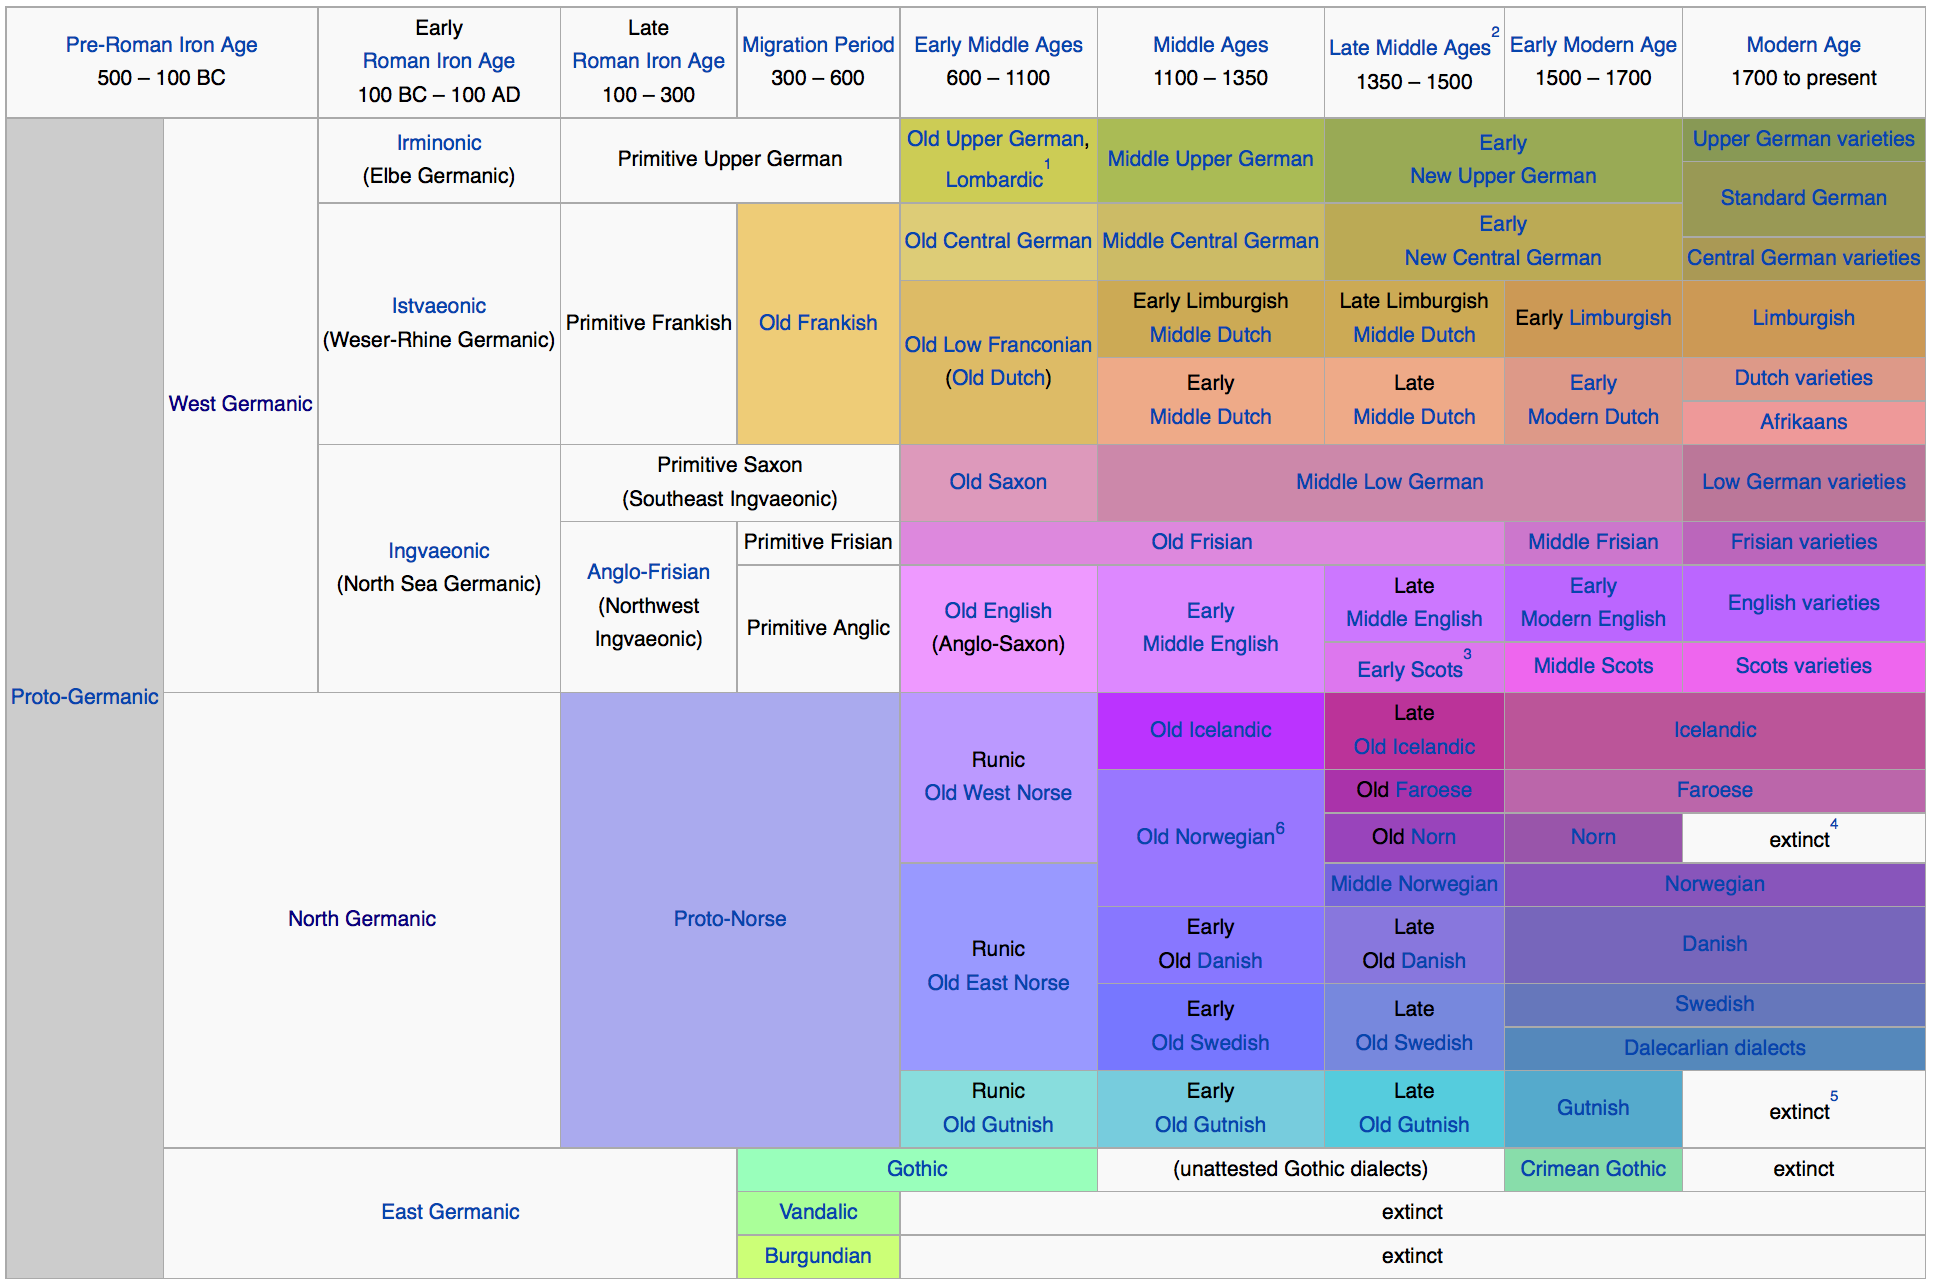
\includegraphics[width=.9\textheight]{Pictures/germanic-wikipedia}
%\end{sideways}
\begin{sideways}
\scalebox{.72}{%
% \begin{forest}forked edges, for tree={grow'=0, child anchor=west, parent anchor=east, align=center}
% [Proto-Germanic\il{Germanic!Proto-}
%     [Northwest Germanic\il{Germanic!Northwest}
%         [North Germanic\il{Germanic!North}, tier=preroman
%             [Old Norse\il{Norse!Old}
%                 [West Norse\il{Norse!West}, tier=premodern
%                     [\ili{Icelandic}, tier=modern]
%                     [\ili{Farocese}, tier=modern]
%                     [\ili{Norwegian}, tier=modern
%                         [\ili{Nynorsk}]
%                     ]
%                 ]
%                 [East Norse\il{Norse!East}
%                     [\ili{Danish}, tier=modern
%                         [\ili{Bokmål}]
%                     ]
%                     [\ili{Swedish}, tier=modern]
%                 ]
%              ]   
%         ]
%         [West Germanic\il{Germanic!West}, tier=preroman
%             [North Sea Germanic\il{Germanic!North Sea}\\(Ingvaeonic)
%                 [Anglo-Frisian\il{Frisian!Anglo-}
%                         [\ili{English}, tier=modern]
%                         [\ili{Frisian}, tier=modern]
%                 ]        
%                 [Old Saxon\il{Saxon!Old}
%                     [Low German\il{German!Low}, tier=modern]
%                 ]
%             ]
%             [\ili{Franconian}\\(Istvaeonic)
%                 [Low Franconian\il{Franconian!Low}, tier=middleages
%                     [Middle Dutch\il{Dutch!Middle}, tier=latemiddleages
%                         [\ili{Dutch}, tier=modern]
%                         [\ili{Afrikaans}, tier=modern]
%                     ]
%                 ]
%                 [High Franconian\il{Franconian!High}, tier=middleages, name=franconian
%                 ]
%             ]
%             [Alpine Germanic\il{Germanic!Alpine}\\(Irminonic)
%                 [\ili{Alemannic}\\\small{(Upper German\il{German!Upper})}, tier=middleages, name=alemannic
%                 	[Middle High\\German\il{German!Middle High}, tier=latemiddleages, no edge, name=mhg 
%                 		[High German\il{German!High}, tier=modern]
%                 		[PA German\il{Pennsylvania German}, tier=modern]
%                 		[\ili{Yiddish}, tier=modern]
%                 	]
%                 ]               
%                 [\ili{Bavarian}\\\small{(Upper German)\il{German!Upper}}, tier=middleages, name=bavarian]
%             ]
%         ]
%     ]    
%     [East Germanic\il{Germanic!East},  tier=preroman
%         [\ili{Gothic} (and others)]
%     ]
% ]
% {\draw[black] (franconian.east)--(mhg.west);}
% {\draw[black] (bavarian.east)--(mhg.west);}
% {\draw[black] (alemannic.east)--(mhg.west);}
% \end{forest}}
\begin{forest}forked edges, for tree={grow'=0, child anchor=west, parent anchor=east, align=center}
[Proto-Germanic
    [Northwest Germanic
        [North Germanic, tier=preroman
            [Old Norse
                [West Norse, tier=premodern
                    [Icelandic, tier=modern]
                    [Faroese, tier=modern]
                    [Norwegian, tier=modern
                        [Nynorsk]
                    ]
                ]
                [East Norse
                    [Danish, tier=modern
                        [Bokmål]
                    ]
                    [Swedish, tier=modern]
                ]
             ]   
        ]
        [West Germanic, tier=preroman
            [North Sea Germanic\\(Ingvaeonic)
                [Anglo-Frisian
                        [English, tier=modern]
                        [Frisian, tier=modern]
                ]        
                [Old Saxon
                    [Low German, tier=modern]
                ]
            ]
            [Franconian\\(Istvaeonic)
                [Low Franconian, tier=middleages
                    [Middle Dutch, tier=latemiddleages
                        [Dutch, tier=modern]
                        [Afrikaans, tier=modern]
                    ]
                ]
                [High Franconian, tier=middleages, name=franconian
                ]
            ]
            [Alpine Germanic\\(Irminonic)
                [Alemannic\\\small{(Upper German)}, tier=middleages, name=alemannic
                	[Middle High\\German, tier=latemiddleages, no edge, name=mhg 
                		[High German, tier=modern]
                		[PA German, tier=modern]
                		[Yiddish, tier=modern]
                	]
                ]               
                [Bavarian\\\small{(Upper German)}, tier=middleages, name=bavarian]
            ]
        ]
    ]    
    [East Germanic,  tier=preroman
        [Gothic (and others)]
    ]
]
{\draw[black] (franconian.east)--(mhg.west);}
{\draw[black] (bavarian.east)--(mhg.west);}
{\draw[black] (alemannic.east)--(mhg.west);}
\end{forest}}
\end{sideways}
% Index entries have to be outside the figure if/since memoize is used
\il{Deutsch!Mittelhoch-}\il{Deutsch!Ober-}\il{Deutsch!Mittelhoch-}\il{Deutsch!Ober-}\il{Bairisch}\il{Germanisch!Alpen-}\il{Afrikaans}%
\il{Alemannisch}\il{Germanisch!Ur-}\il{Germanisch!Nordwest-}\il{Germanisch!Nord-}\il{Nordisch!Alt-}\il{Nordisch!West-}\il{Isländisch}%
\il{Färöisch}\il{Norwegisch}\il{Nynorsk}\il{Nordisch!Ost-}\il{Dänisch}\il{Bokmål}\il{Schwedisch}\il{Germanisch!West-}\il{Germanisch!Nordsee-}%
\il{Friesisch!Angel-}\il{Englisch}\il{Friesisch}\il{Sächsisch!Alt-}\il{Deutsch!Nieder-}\il{Fränkisch}\il{Fränkisch!Nieder-}\il{Niederländisch!Mittel-}%
\il{Niederländisch}\il{Afrikaans}\il{Fränkisch!Hoch-}\il{Alemannisch}\il{Deutsch!Hoch-}\il{Pennsylvania-Deutsch}\il{Jiddisch}\il{Bairisch}%
\il{Germanisch!Ost-}\il{Gotisch}%
\caption{\label{fig-history-relations-germanic}Entwicklung der germanischen Sprachen nach
  \citew[\page 8]{Harbert2006a-u}}
\end{figure}
Das \ili{Germanisch}e wird in Ost\il{Germanisch!Ost}-, West\il{Germanisch!West}- und
Nord\il{Germanisch!Nord}germanisch eingeteilt. Das Ostgermanische existierte in Form des \ili{Gotisch}en
bis etwa 1800 auf der Krim (Krimgotisch\il{Gotisch!Krim-}) und ist heute vollständig ausgestorben.

Das Westgermanische\il{Germanisch} besteht aus
\begin{itemize}
\item \ili{Deutsch},
\item \ili{Jiddisch},
\item \ili{Luxemburgisch},
\item \ili{Pennsylvania-Dutch},
\item Niederdeutsch\il{Deutsch!Nieder-}, % Plattdeutsch or Niederdeutsch
\item \ili{Plautdietsch} (auch Mennonitisches Niederdeutsch\il{Deutsch!Mennonitisches Nieder-} genannt), %
\item \ili{Niederländisch},
\item \ili{Afrikaans},
\item \ili{Friesisch} und
\item \ili{Englisch}.
\end{itemize}
%\largerpage
Die nordgermanischen\il{Germanisch} Sprachen sind:
\begin{itemize}
\item \ili{Dänisch},
\item \ili{Schwedisch},
\item \ili{Norwegisch},
\item \ili{Isländisch} und
\item \ili{Färöisch}.
\end{itemize}

\noindent
Tabelle~\vref{tab-words-germanic} zeigt, wie ähnlich die Wörter aus dem Grundwortschatz der germanischen\il{Germanisch}
Sprachen sind:
\begin{table}
\centerfit{%
\begin{tabular}{lllllllll}
\hline\hline
\ili{Niederländisch} & vader  & vier    & vol    & huis  & bruin  & uit & kruid     & muis\\
\ili{Deutsch}        & Vater  & vier    & voll   & Haus  & braun  & aus & Kraut     & Maus\\
\ili{Englisch}       & father & four    & full   & house & brown  & out & crowd (?) & mouse\\
\ili{Friesisch}      & –      & fjouwer & fol    & hûs   & brún   & út  & krûd      & mûs\\
\ili{Schwedisch}     & fader  & fyra    & full   & hus   & brun   & ut  & krut      & mus\\
\ili{Dänisch}        & fader  & fire    & fuld   & hus   & brun   & ud  & krudt     & mus\\
\ili{Norwegisch}     & far    & fire    & full   & hus   & brun   & ut  & krydder   & mus\\
\ili{Isländisch}     & faðir  & fjórir  & fullur & hús   & brúnn  & út  & –         & mús\\
\hline\hline
\end{tabular}
}
\caption{\label{tab-words-germanic}Wörter aus dem Grundwortschatz einiger germanischer Sprachen}
\end{table}

%% \section{Stammbaum der germanischen Sprachen}
%% \includegraphics[width=\textwidth]{Pictures/stammbaum-germanisch}
%% aus \citew[S.\,251]{Bussmann2002a}





\section{Die drei Zweige der germanischen Familie}

Das \ili{Urgermanisch}e entwickelte sich etwa im ersten Jahrhundert n.\,Chr. zu den drei Hauptzweigen Ost-, West- und Nordgermanisch\il{Germanisch}. Die Gründe für diese Entwicklung waren inhärente Variationen in den jeweiligen
Dialekten, Migration (Sprachkontakt) und Standardisierung. Das vorliegende Buch behandelt die Struktur der
germanischen\il{Germanisch} Standardsprachen. Dieser Abschnitt ist in drei Unterabschnitte gegliedert, die den
drei germanischen Hauptzweigen entsprechen. Ich werde die historischen Entwicklungen skizzieren, die zu den
heute gesprochenen Sprachen geführt haben. Viele der Details, die in Abbildung~\ref{fig-history-relations-germanic} dargestellt sind, werden dabei ignoriert.



\subsection{Ostgermanisch}

Es\il{Germanisch!Ost|(} wird oft behauptet, dass die Goten von den dänischen\il{Dänisch} Inseln und aus Südschweden auf das europäische Festland
auswanderten, doch neuere Forschung, die archäologische Funde berücksichtigt, geht davon aus, dass sie
im ersten Jahrhundert n.\,Chr. auf dem europäischen Festland gegenüber Skandinavien rund um die Weichsel lebten und später nach Süden in das Hinterland des
Schwarzen Meeres zogen \citep[20--30]{Heather1999a-u}. In dieser Zeit standen sie in Kontakt mit den Vandalen\il{Vandalisch} und anderen Stämmen.
%emigrated from the \ili{Danish} islands and South Sweden around 100 BCE and met the
%Vandals and other tribes.\itdopt{%
%Walkden: Most current historical research (since e.g. Heather 1998, The Goths, 25–30) rejects the
%idea that the Goths originated in Scandinavia, and put their earliest origin around the Vistula. Not
%a crucial point in the context of this book, but may be worth changing.
%}
Das \ili{Gotisch}e, \ili{Vandalisch}e und \ili{Burgundisch}e sowie einige kleinere Sprachen bildeten den ostgermanischen Zweig, von dem nur das \ili{Gotisch}e überliefert wurde.
Nach dem Zerfall der gotischen\il{Gotisch} Reiche starb das \ili{Gotisch}e aus. Auf der Halbinsel Krim gab es einige Überreste
bis etwa 1800. Der westgotische\il{Gotisch} Bischof Wulfila (oder vielmehr ein von ihm geleitetes Team, siehe
\citealt{Ratkus2018a-u}) übersetzte die Bibel ins \ili{Gotisch}e. Die
bekannteste Fassung davon ist das Fragment Codex Argenteus, das sich in der Universitätsbibliothek von
Uppsala befindet. Abbildung~\vref{fig-Wulfila-Bibel} zeigt ein Bild davon.\footnote{
Übernommen aus Wikipedia: \url{http://de.wikipedia.org/wiki/Bild:Wulfila_bibel.jpg}. 19.10.2014.
}
\begin{figure}
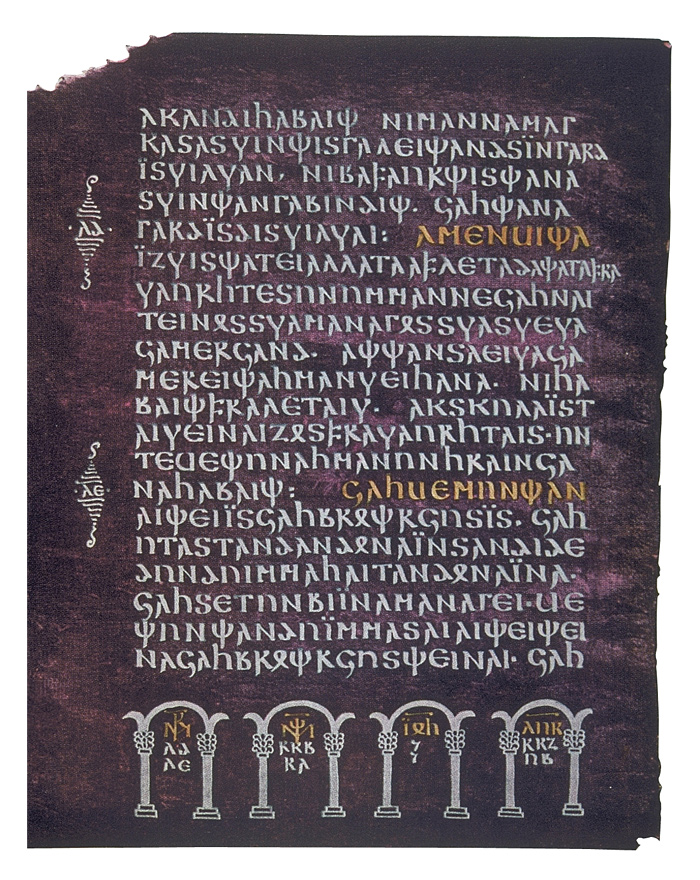
\includegraphics[width=53mm]{Pictures/Wulfila_bibel}
\caption{\label{fig-Wulfila-Bibel}Die Wulfila-Bibel (Codex Argenteus), Bild aus Wikipedia}
\end{figure}
\il{Germanisch!Ost|)}


\subsection{Nordgermanisch}

Die\il{Germanisch!Nord|(} ersten Schriften auf Runensteinen gehen auf das sechste Jahrhundert zurück. Die Sprache der Wikinger
(800--1050) war recht homogen, und erst nach dieser Epoche begannen sich zwei Zweige zu
entwickeln: der ostskandinavische\il{Skandinavisch!Ost} Zweig mit Altdänisch\il{Dänisch!Alt-} und Altschwedisch\il{Schwedisch!Alt-} und der westskandinavische\il{Skandinavisch!West} Zweig
mit Altnorwegisch\il{Norwegisch!Alt-} und Altisländisch\il{Isländisch!Alt-}.


\subsubsection{Dänisch}

Das \ili{Dänisch}e (dansk) ist die Amtssprache des
\href{https://en.wikipedia.org/wiki/Denmark}{Königreichs Dänemark} und die zweite Amtssprache der
Färöer-Inseln und Grönlands, wobei das \ili{Grönländisch}e die erste Amtssprache
Grönlands ist. Das \ili{Dänisch}e hat etwa 5,5 Millionen Sprecher*innen. Etwa 50.000 Sprecher*innen leben in \href{https://en.wikipedia.org/wiki/Schleswig-Holstein}{Schleswig-Holstein}, dem nördlichsten der Bundesländer Deutschlands.
Das \ili{Dänisch}e ist die skandinavische\il{Skandinavisch} Sprache, die sich am weitesten von den gemeinsamen skandinavischen\il{Skandinavisch} Wurzeln entfernt hat.


\subsubsection{Schwedisch}

Das \ili{Schwedisch}e (svenska) ist die Amtssprache in Schweden mit etwa 8,5 Millionen Muttersprachler*innen. Es ist
die Erstsprache von etwa 300.000 schwedischsprachigen\il{Schwedisch} Finnen in Finnland. Bis in die Zeit der
Wikinger waren das \ili{Dänisch}e und das \ili{Schwedisch}e kaum zu unterscheiden. Ab etwa 800 begannen sie
auseinanderzudriften. Seit etwa 1300 gibt es deutliche Unterschiede.



\subsubsection{Isländisch}


Das \ili{Isländisch}e (íslenska) wird seit der Besiedlung Islands vor über 1000 Jahren dort
gesprochen. Mit dem \ili{Färöisch}en gehört es zu den westskandinavischen Sprachen\il{Skandinavisch!West-}.
% Wikipedia 23.10.2014
Es gibt etwa 325.000 Muttersprachler*innen. 97\,\% der isländischen\il{Isländisch} Bevölkerung (325.000) haben das \ili{Isländisch}e als
Muttersprache, und es gibt große Gruppen von Muttersprachler*innen in Dänemark, den USA und Kanada
(insgesamt etwa 15.000).
Es gibt weniger Variation als in anderen germanischen\il{Germanisch} Sprachen (keine Dialekte).
%AZ that is too strong there is actually quite a bit of variation but maybe it is correct to say that there is less variation than in other \ili{Germanic} languages
Die Sprache ist konservativ in dem Sinne, dass das \ili{Isländisch}e
diejenige unter den germanischen\il{Germanisch} Sprachen ist, die den germanischen\il{Germanisch} Wortschatz und die Flexion am besten bewahrt hat.
Am Anfang gab es kaum Unterschiede zwischen dem \ili{Norwegisch}en und dem \ili{Isländisch}en, aber
% The \ili{Dano-Norwegian}, then later \ili{Danish} rule of Iceland from 1536 to 1918 had little effect on the
% evolution of \ili{Icelandic} (in contrast to the \ili{Norwegian} language), which remained in daily use among
% the general population.
% AZ: when?
ab etwa 1100 drifteten die Sprachen auseinander. Dieser Prozess setzte sich auch aufgrund des dänischen\il{Dänisch}
Einflusses fort, und heutzutage ähnelt das \ili{Norwegisch}e mehr dem \ili{Dänisch}en als dem
\ili{Isländisch}en. Es gibt viele isländische\il{Isländisch} Schriftzeugnisse.

\subsubsection{Norwegisch}

%\largerpage
Es gibt zwei Standardvarietäten des \ili{Norwegisch}en (norsk): Dänisch-Norwegisch\il{Norwegisch!Dänisch-} (bokmål) und Neunorwegisch\il{Norwegisch!Neu-} (nynorsk, landsmål).
Beide sind Amtssprachen Norwegens.
% and are used in parallel\itdopt{AZ: not clear what that means}.
Es gibt etwa 4,3 Millionen Sprecher*innen.
Von 1380 bis 1814 war das \ili{Dänisch}e die Schriftsprache, und in Norwegen wurden lokale Dialekte gesprochen. Daraus entwickelte sich der Bokmål-Standard.
Ivar Aasen (1813--1896) entwickelte mit \ili{Nynorsk} einen Standard, der weniger vom \ili{Dänisch}en beeinflusst ist. \ili{Nynorsk} erhielt 1885 offiziellen Status. Das \ili{Bokmål} `Buchsprache' ist die Erstsprache der meisten
Norweger.

\subsubsection{Färöisch}

Das \ili{Färöisch}e (føroyskt) ist -- neben dem \ili{Dänisch}en -- Amtssprache der Färöer-Inseln. Es
gibt etwa 47.000 Sprecher*innen. Die Färöer-Inseln gehören seit 1816 zu Dänemark. Seit 1948 sind sie
ein selbstverwaltetes Land innerhalb des \href{https://en.wikipedia.org/wiki/Danish_Realm}{dänischen\il{Dänisch} Reichs}.
Das \ili{Färöisch}e hat einen starken dänischen\il{Dänisch} Einfluss. Die erste handschriftliche Überlieferung stammt erst aus dem Jahr 1773, und
auch nach diesem Datum gibt es nicht viele schriftliche Zeugnisse.%
%AZ i would leave this out: (in contrast to \ili{Icelandic}).And put something in the \ili{Icelandic} section
\il{Germanisch!Ost|)}

\subsection{Westgermanisch}


Die\il{Germanisch!West|(} Meinungen zu der Frage, ob sich das Westgermanische aus einer einzigen Quelle entwickelt hat oder nicht, gehen auseinander. Einige Autoren
nehmen an, dass die westgermanischen\il{Germanisch} Sprachen keine gemeinsame Wurzel haben, sondern sich aus den
folgenden drei nicht verwandten Zweigen von Dialektgruppen entwickelt haben (zum Beispiel \citealp[\page 17--18]{Robinson1992a-u} und
\citealp[\page 9]{HvDA94a}):
\begin{itemize}
\item Nordseegermanisch\il{Germanisch!Nordsee} %(Ingvaeonic, ancestral to \ili{Anglo-Frisian} and also Old Saxon)
\item Weser-Rhein-Germanisch\il{Germanisch!Weser-Rhein} %(Istvaeonic, ancestral to Old \ili{Frankish},
                                %its successors \ili{Low Franconian} and several dialects of Old High \ili{German})
\item Elbgermanisch\il{Germanisch!Elb-} %(Irminonic, ancestral to several dialects of Old High \ili{German}, most probably including the extinct \ili{Langobardic} language).
\end{itemize}
Andere Autoren nehmen an, dass diese drei Zweige einen gemeinsamen Vorfahren hatten (siehe
Abbildung~\ref{fig-history-relations-germanic}), und manche lehnen es ab, das Westgermanische überhaupt in
drei Unterzweige zu unterteilen \citep{Stiles2013a-u}.
Es gibt keine eindeutige Zuordnung dieser Dialektgruppen zu den heute gesprochenen Sprachen.%

%\largerpage
\subsubsection{Deutsch}

Das \ili{Deutsch}e ist die Amtssprache von
\begin{itemize}
\item Deutschland (etwa 80 Millionen Sprecher*innen),
\item Österreich (etwa 7,5 Millionen Sprecher*innen),
\item Liechtenstein (etwa 15.000 Sprecher*innen),
\item der Schweiz (4,2 Millionen von 6,4 Millionen Einwohnern der Schweiz),
\item Norditalien/Südtirol (etwa 270.000 Sprecher*innen),
\item Belgien (etwa 65.000 Sprecher*innen) und
\item Luxemburg (etwa 360.000 Sprecher*innen).
\end{itemize}
Neben dem \ili{Deutsch}en hat Luxemburg auch das \ili{Luxemburgisch}e und das \ili{Französisch}e als
Amtssprachen.
%Poland 50,000 native speakers.
Es gibt weitere Länder, in denen das \ili{Deutsch}e eine Nationalsprache oder eine nationale oder regionale
Minderheitensprache ist: Brasilien, Tschechien, Dänemark, Ungarn, Namibia, Polen, \ili{Rumänien}, Russland und die Slowakei.

% There are about 97 million speakers of \ili{German}, about, 90 of those are native speakers and 7 million
% have \ili{German} as their second language.
% % = Migrationshintergrund
% % Quelle Wikipedia 15.10.2013
% Approximately 80 million speakers speak \ili{German} as a foreign language, about 55 Million of these live
% in the \ili{European} Union.%AZ It is a bit awkward to get these details for \ili{German} but not for all the other languages

Es gibt drei nationale Hauptvarianten (Deutschland, Österreich, Schweiz). In anderen Ländern ist das \ili{Deutsch}e
%AZ leave out usually
eine Minderheitensprache. Es gibt zwei große Dialektgruppen: das Niederdeutsche\il{Deutsch!Nieder-}
(Plattdütsch, Plattdütsk, Plattduitsch, 
Nedderdütsch; im Standarddeutschen: Platt\-deutsch oder Nie\-der\-deutsch%
%AZ this is clear as mud: do you
%want to say that \ili{Dutch} is part of low Saxon or as most people do
%that low saxon are the dialects of \ili{German} that are spoken in in the Netherlands? I would say:
%Nedersaksisch or Low Saxon, a group of dialects spoken in the Netherlands, southern Danmark and
%northwestern Germany
% Well, the areas in which Low Saxon is spoken overlap with national border. I speak about langauges
% spoken in these national borders here.
) und das Hochdeutsche\il{Deutsch!Hoch-} (Varietäten des \ili{Deutsch}en, die südlich der Benrather und Uerdinger
Isoglossen gesprochen werden).
%\itdopt{Stefan: fix}
%\todostefan{more}

% Wikipedia
%% The High \ili{German} languages or High \ili{German} dialects (\ili{German}: Hochdeutsche Dialekte) comprise the varieties of \ili{German} spoken south of the Benrath and Uerdingen isoglosses in central and southern Germany, Austria, Liechtenstein, Switzerland, and Luxembourg as well as in neighboring portions of Belgium (Eupen-Malmedy) and the Netherlands (Southeast Limburg), France (Alsace and northern Lorraine), Italy (South Tyrol), and Poland (Upper Silesia). They are also spoken in diaspora in \ili{Romania}, Russia, the United States, Brazil, Argentina, Chile, and Namibia.

%% The High \ili{German} languages are marked by the High \ili{German} consonant shift, separating them from Low \ili{German} and Low \ili{Franconian} (\ili{Dutch}) within the continental West \ili{Germanic} dialect continuum.


%% Wikipedia

%% \ili{Middle} Low \ili{German} was the lingua franca of the Hanseatic League. It was the predominant language in \ili{Northern} Germany. This changed in the 16th century: in 1534 the Luther Bible was published. This translation is considered to be an important step towards the evolution of the Early New High \ili{German}. It aimed to be understandable to a broad audience and was based mainly on Central and Upper \ili{German} varieties. The Early New High \ili{German} language gained more prestige than Low \ili{German} and became the language of science and literature. Around the same time, the Hanseatic league, based around northern ports, lost its importance as new trade routes to Asia and the Americas were established, while the most powerful \ili{German} states of that period were located in \ili{Middle} and Southern Germany.

%% The 18th and 19th centuries were marked by mass education in Standard \ili{German} in schools. Gradually Low \ili{German} came to be politically viewed as a mere dialect spoken by the uneducated. Today Low Saxon can be divided in two groups: Low Saxon varieties with a reasonable standard \ili{German} influx[clarification needed] and varieties of Standard \ili{German} with a Low Saxon influence known as Missingsch. Sometimes, Low Saxon and Low \ili{Franconian} varieties are grouped together because both are unaffected by the High \ili{German} consonant shift. However, the proportion of the population who can understand and speak it has decreased continuously since World War II.


%% Wikipedia
%% High \ili{German} is divided into Central \ili{German}, High \ili{Franconian} (a transitional dialect), and Upper \ili{German}. Central \ili{German} dialects include \ili{Ripuarian}, Moselle \ili{Franconian}, Rhine \ili{Franconian}, Central Hessian, East Hessian, North Hessian, Thuringian, \ili{Silesian} \ili{German}, Lorraine \ili{Franconian}, \ili{Mittelalemannisch}, North Upper Saxon, High \ili{Prussian}, Lausitzisch-Neumärkisch and Upper Saxon. It is spoken in the southeastern Netherlands, eastern Belgium, Luxembourg, parts of France, and parts of Germany roughly between the River Main and the southern edge of the Lowlands. Modern Standard \ili{German} is mostly based on Central \ili{German}, although the common (but not linguistically correct) \ili{German} term for modern Standard \ili{German} is Hochdeutsch, that is, High \ili{German}.

%% The Moselle \ili{Franconian} varieties spoken in Luxembourg have been officially standardised and institutionalised and are usually considered a separate language known as \ili{Luxembourgish}.

%% The two High \ili{Franconian} dialects are East \ili{Franconian} and South \ili{Franconian}.

%% Upper \ili{German} dialects include \ili{Northern} Austro-Bavarian, Central Austro-Bavarian, Southern Austro-Bavarian, Swabian, East \ili{Franconian}, High \ili{Alemannic} \ili{German}, Highest \ili{Alemannic} \ili{German}, Alsatian and Low \ili{Alemannic} \ili{German}. They are spoken in parts of the Alsace, southern Germany, Liechtenstein, Austria, and the \ili{German}-speaking parts of Switzerland and Italy.

%% Wymysorys is a High \ili{German} dialect of Poland native to Wilamowice, and Sathmarisch and Siebenbürgisch are High \ili{German} dialects of \ili{Romania}. The High \ili{German} varieties spoken by Ashkenazi Jews (mostly in the former \ili{Russian} Empire) have several unique features, and are usually considered as a separate language, \ili{Yiddish}. It is the only \ili{Germanic} language that does not use the \ili{Latin} script as the basis of its standard alphabet.


\subsubsection{Jiddisch}

Das \ili{Jiddisch}e ist eine von vielen Sprachen, die in der jüdischen Diaspora gesprochen werden. Was die Sprecher*innenzahl betrifft,
gibt es keine verlässlichen Zahlen: Einige Quellen gehen davon aus, dass
1,5 Millionen Menschen diese Sprache aktiv oder passiv sprechen, wobei nur 500.000 Sprecher*innen die Sprache
aktiv im Alltag verwenden. Andere Quellen gehen von 4 Millionen
Sprecher*innen aus. In jedem Fall war die Zahl der \ili{Jiddisch}sprecher*innen vor 100 Jahren deutlich
höher: \citet[\page 6]{Birnbaum1915a-u} schätzte die Zahl der Sprecher*innen auf bis zu 12 Millionen. Die meisten von
ihnen lebten im Gebiet der Sowjetunion (über 7 Millionen), und es gab größere Gemeinschaften in den Vereinigten Staaten (über 2 Millionen), in Österreich-Ungarn
(1,5 bis 2 Millionen), \ili{Rumänien} (über 250.000), Großbritannien
(250.000), Palästina, Argentinien und Kanada (jeweils etwa 100.000). Siehe auch \citew{Schaefer2023a} für
Schätzungen der Sprecher*innenzahlen und weitere Literaturhinweise.

%7 million speakers of \ili{Yiddish} lived in Europe, most of them in the area of the Sovjet Union and in
%Austria-Hungary. At most 75,000 \ili{Yiddish} speakers are left in Western Europe.
Das \ili{Jiddisch}e hat seine Wurzeln
im mittelalterlichen \ili{Deutsch} mit Einflüssen aus dem \ili{Hebräisch}en und \ili{Aramäisch}en. Es ist außerdem von
romanischen Sprachen beeinflusst, insbesondere von altfranzösischen\il{Französisch!Alt-} und italienischen\il{Italienisch} Varietäten.


\subsubsection{Pennsylvania-Deutsch}

\ili{Pennsylvania-Deutsch} (\ili{Pensilfaanish}, Pensilfaanish Deitsch), das auch als \emph{Pennsylvania Dutch} bekannt ist, hat etwa 300.000
Muttersprachler*innen, die hauptsächlich in den USA leben. Die wichtigsten Regionen sind Pennsylvania, Ohio und
Indiana. Das Pennsylvania-Deutsche hat sich aus pfälzischen Dialekten entwickelt, die von
Einwanderern gesprochen wurden, die im 17.\ und 18.\ Jahrhundert nach Nordamerika kamen.
% Die ersten um 1683
Angehörige verschiedener protestantischer Religionsgemeinschaften (Mennoniten, Pietisten und so weiter) verließen Europa aus religiösen Gründen,
doch später folgten Einwanderer, die aus wirtschaftlichen Gründen kamen. Die Sprache wird heutzutage
hauptsächlich von Amischen und Mennoniten gesprochen. 




\subsubsection{Niederländisch}

Das \ili{Niederländisch}e (Nederlands) ist die Amtssprache der Niederlande und hat in diesem Land etwa 15 Millionen Sprecher*innen. \ili{Niederländisch} ist außerdem eine der Amtssprachen Belgiens mit etwa 6 Millionen Sprecher*innen.
%AZleave out: ; almost 4 million Walloones).
Es ist die alleinige Amts- und Unterrichtssprache in Surinam
%AZ leave out: which is independent since 1975,
% 60% of the population speak it as their mother tongue % wikipedia
% 24% speak it as a second language
sowie in \href{https://en.wikipedia.org/wiki/Aruba}{Aruba} und den \href{https://en.wikipedia.org/wiki/Netherlands_Antilles}{Niederländischen Antillen}.

%In Aruba, Curaçao and Sint Maarten, all parts of the Kingdom of the Netherlands, \ili{Dutch} is the official language but spoken as a first language by only 7% to 8% of the population,[56] although most native-born people on the islands can speak the language since the education system is in \ili{Dutch} at some or all levels.[57] The lingua franca of Aruba, Bonaire and Curaçao is Papiamento, a creole language that originally developed among the slave population. The population of the three northern Antilles, Sint Maarten, Saba, and Sint Eustatius, is predominantly \ili{English}-speaking.[44]

\subsubsection{Afrikaans}

Das \ili{Afrikaans} ist seit 1925 eine der Amtssprachen Südafrikas, das elf Amtssprachen hat.
Es gibt etwa 6,4 Millionen Muttersprachler*innen in Südafrika, was etwa 15\,\% der Bevölkerung entspricht,
und 150.000 in Namibia. Das \ili{Afrikaans} hat sich seit dem 17. Jahrhundert aus niederländischen\il{Niederländisch} Dialekten entwickelt und wird
seit irgendwann zwischen 1775 und 1850 als eigenständige Sprache angesehen
%\parencites[\page 99]{denBesten2012b-u}
\citep[\page 272]{denBesten2012a-u}.
% Oft wird gesagt, dass ab ca. 1775 von '\ili{Afrikaans}' gesprochen werden kann (Den Besten spricht aber noch vom 'Proto-Afrikaans'). Die Übergänge vom Kap-Niederländischen zum \ili{Afrikaans} sind natürlich fließend, aber um die Zeit herum, gibt es doch schon genügend dokumentierte Unterschiede, um zu sagen, dass \ili{Afrikaans} eine eigenständige Sprache geworden ist. Allerspätestens ab Mitte des 19. Jahhunderts ist dann aber auf jeden Fall eine eigene Sprache anzusetzen; da sind sich alle einig. Und 1925 wird das dann ja auch offizielle Amtssprache. 
Die verschiedenen in der Region gesprochenen afrikanischen Sprachen standen in Wechselwirkung mit dem \ili{Afrikaans}.
%AZ leave out: and its origins and resulted in a structural simplification in comparison to \ili{Dutch}
Heute hat das \ili{Englisch}e einen starken Einfluss.



\subsubsection{Friesisch}

Die drei Varietäten des \ili{Friesisch}en sind untereinander nicht verständlich. Es gibt das Nordfriesische\il{Friesisch!Nord-}, das von
etwa 10.000 Sprecher*innen hauptsächlich auf den nordfriesischen\il{Friesisch} Inseln Amrum, Sylt und Helgoland gesprochen wird. Das Ostfriesische\il{Friesisch!Ost-}
ist mit Ausnahme des \ili{Saterfriesisch}en ausgestorben, das in den drei Dörfern des Saterlandes
(Landkreis Cloppenburg) von zwischen 1.000 und 2.500 Menschen gesprochen wird.
% https://www.taz.de/!5834717 Inseln
Das Westfriesische\il{Friesisch!West-} wird in der nördlichen niederländischen\il{Niederländisch} Provinz Fryslân (Friesland) gesprochen und hat etwa 350.000
Muttersprachler*innen.



\subsubsection{Englisch}

Weltweit hatte das \ili{Englisch}e Ende des 20. Jahrhunderts etwa 570 Millionen Sprecher*innen
(337 Millionen Muttersprachler*innen, 235 Millionen Sprecher*innen mit \ili{Englisch} als \isi{Zweitsprache}\footnote{%
  Der Terminus \emph{Zweitsprache} bezeichnet eine Sprache, die Sprecher*innen im
  Alltag verwenden, weil diese Sprache in der Umgebung, in der sie leben, gesprochen wird. Ein Beispiel wären Sprecher*innen mit
  Türkisch als Erstsprache, die in Deutschland leben. Die deutsche Tradition unterscheidet
  \emph{Zweitsprache} von \emph{Fremdsprache}.%
}). Die Länder mit den meisten Muttersprachler*innen sind im Folgenden aufgeführt:
\begin{itemize}
\item USA: 227 Millionen,
\item Großbritannien: 57 Millionen,
\item Nigeria: 43 Millionen,
\item Kanada: 24 Millionen,
\item Australien: 17 Millionen,
\item Irland: 3,5 Millionen,
\item Neuseeland: 3,2 Millionen.
\end{itemize}
Es gibt viele nationale Varianten, die sich hauptsächlich in der Aussprache unterscheiden.
Zwischen 1 und 1,5 Milliarden Menschen verfügen über aktive oder passive Kenntnisse des \ili{Englisch}en.
Das \ili{Englisch}e ist in 59 Staaten Amtssprache. Es ist die wichtigste Wissenschaftssprache.%
\il{Germanisch!West|)}


\questions{
\begin{enumerate}
\item Nennen Sie mindestens zehn germanische Sprachen.
\end{enumerate}

}


%      <!-- Local IspellDict: de_DE -->


%% -*- coding:utf-8 -*-

\settowidth\jamwidth{(\ili{Deutsch})}

\chapter{Phänomene}

Dieses Kapitel befasst sich mit der Variation in den germanischen\il{Germanisch} Sprachen in dem Bereich, der oft als Kerngrammatik
bezeichnet wird, das heißt mit Sätzen vom Typ \emph{Karl liebt Maria}.\footnote{%
  \citet[\page 7--8]{Chomsky81a} schlägt vor, Grammatiken natürlicher Sprachen in einen "`Kern"' und eine "`Peripherie"' zu unterteilen.
Alle regelmäßigen Teile gehören zum Kern. Die Kerngrammatik einer Sprache wird als eine Instanz der
Universalgrammatik (UG) angesehen, der genetisch determinierten angeborenen Sprachfähigkeit des Menschen. Idiome
und andere unregelmäßige Teile einer Sprache gehören zur Peripherie. Dieses Buch befasst sich mit Phänomenen,
die üblicherweise als Teil des Kerns angesehen werden, ohne diese Kern/Peripherie-Unterscheidung anzunehmen und ohne
eine UG anzunehmen \citep{MuellerKernigkeit,MuellerCoreGram}.
} Wir werden uns Unterschiede in
der Verbstellung (Verb vor Objekt und Objekt vor Verb) ansehen, die Verbzweiteigenschaft, die
alle germanischen\il{Germanisch} Sprachen mit Ausnahme des \ili{Englisch}en haben, die Abfolge von Subjekten und
Objekten zueinander, die Stellung von Adverbialen, die Existenz/Nichtexistenz von
Verbalkomplexen, die Obligatheit/Abwesenheit von Subjekten, das Passiv einschließlich des persönlichen und
unpersönlichen Passivs, Expletivpronomen und verschiedene Möglichkeiten, den \isi{Satztyp} zu markieren, das heißt
zu signalisieren, ob ein bestimmter Satz eine Aussage, eine Frage oder ein eingebetteter Satz ist.

In diesem Kapitel werden die Phänomene vorgestellt, die dann in den
Kapiteln~\ref{chap-valence}--\ref{chap-expletives} detaillierter besprochen und analysiert werden.

Ein Wort der Vorsicht ist hier nötig: Insbesondere die folgenden drei Unterabschnitte sind potenziell
verwirrend. Eine Sprache wie das \ili{Deutsch}e wird als Subjekt-Objekt-Verb-Sprache, als Verbzweitsprache und
als Sprache mit freier Konstituentenabfolge klassifiziert \citep{Haftka96a}. Das klingt widersprüchlich, ist es aber nicht. Die jeweiligen
Klassifikationen beziehen sich auf Eigenschaften von Sprachen, nicht auf die Form einzelner Sätze.

\section{Abfolge von Subjekt, Objekt und Verb}
\label{sec-intro-svo}

Die\is{Abfolge|(}\is{Abfolge!SVO|(}\is{Abfolge!SOV|(} Sprachen der Welt können nach der jeweils
dominanten Abfolge von Subjekt, Objekt und Verb klassifiziert werden \citep{Greenberg63a-u}. Um Sprachen vergleichbar zu machen, wird für eine solche Klassifikation eine sehr allgemeine Definition grammatischer
Funktionen wie Subjekt und Objekt verwendet.
Die Definition basiert auf semantischen Eigenschaften: Subjekte sind diejenigen
Argumente, die agensartig sind, und Objekte sind Argumente, die eher patiensartig sind. Diese Definition
ist nicht immer identisch mit den einzelsprachlichen Definitionen. Zum Beispiel bezieht sich die
einzelsprachliche Definition des Subjekts im \ili{Deutsch}en (und in den germanischen\il{Germanisch} Sprachen im Allgemeinen)
auf Eigenschaften wie den Nominativ\is{Kasus!Nominativ} \citep{Reis82}, Subjekt-Verb-\isi{Kongruenz} und Kontrolle. Wir werden uns damit in
Abschnitt~\ref{sec-subj-properties} genauer befassen. Nach er Definition von Reis ist die Phrase \emph{der
  Aufsatz} in (\mex{1}) das Subjekt, obwohl sie unbelebt und kein Agens ist:
\ea
Der Aufsatz interessiert mich.
\z

\noindent
Abbildung~\vref{fig-sov-wals} zeigt die dominante Abfolge von Subjekt, Objekt und Verb in den Sprachen der Welt.
Nach \citet{Dryer2013a} ist die dominante Abfolge wie folgt definiert:

%Dominante Abfolge (Dryer: Determining Dominant Word Order):
%\largerpage
\begin{quote}
Where a language is shown on one of the word order maps as having a particular order as the dominant
order in the language, this means that it is either the only order possible or the order
that is more frequently used. \citep{Dryer2013a}
\end{quote}
%
%% I base my classification of Macushi here on the frequency counts, and since no order is more than
%% twice as frequent as the next most frequent order, I treat this language as lacking a dominant order
%% of subject, object, and verb.
%
%% Deutsch, Niederländisch und Friesisch sind V2-Sprachen, that is die SVO- und SVAuxOV-Stellungen kommen
%% durch die Voranstellung des Verbs zustande, die eine Funktion hat. Wir zählen diese Sprachen also
%% mit zu den SOV-Sprachen.
%
\begin{figure}
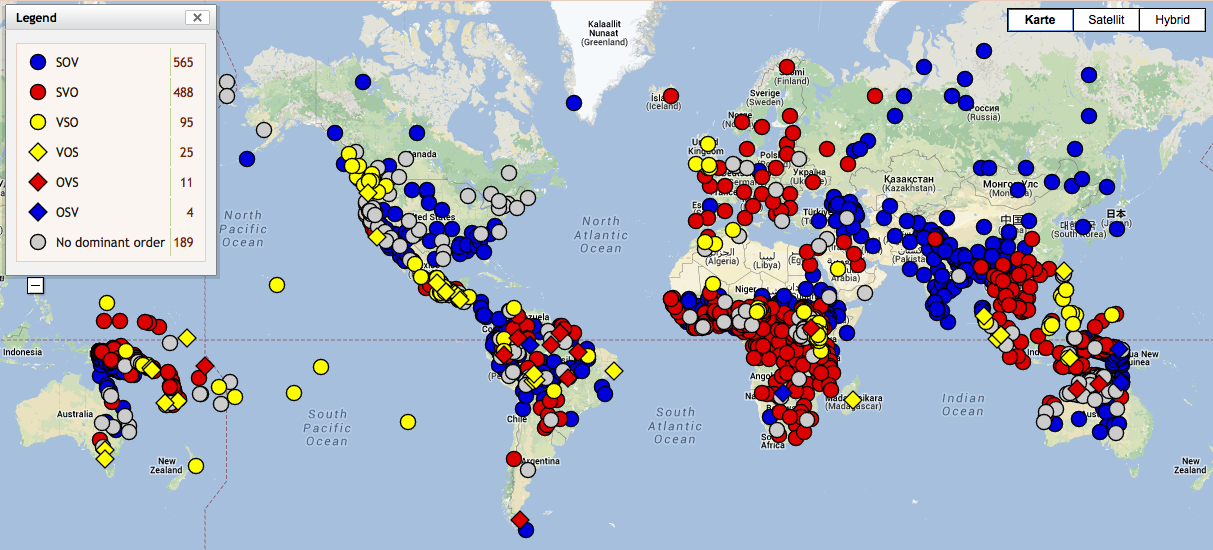
\includegraphics[width=\textwidth]{Pictures/WALS-SOV}
\caption{\label{fig-sov-wals}\citet[Abschnitt~1]{Dryer2013c}: Feature 81A: Order of subject, object and verb, The World Atlas of Language Structures}
\end{figure}

Wenn wir hineinzoomen, um die europäischen Sprachen anzuzeigen, erhalten wir Abbildung~\vref{fig-sov-wals-europe}.
\begin{figure}
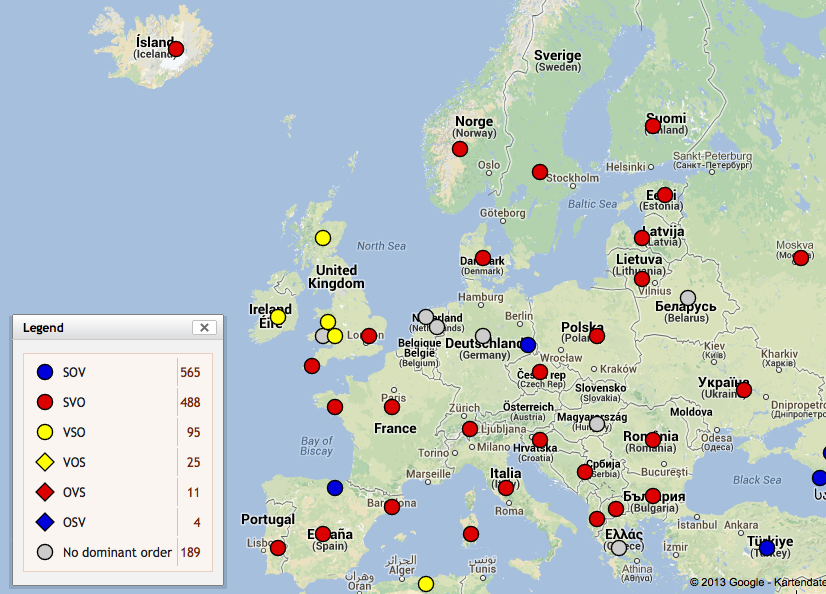
\includegraphics[width=.898\textwidth]{Pictures/WALS-SOV-Europa}
\caption{\label{fig-sov-wals-europe}Dominante Abfolgen von Subjekt, Objekt und Verb in Europa}
\end{figure}
Nach dem WALS sind \ili{Isländisch}, \ili{Norwegisch}, \ili{Schwedisch}, \ili{Dänisch} und \ili{Englisch} SVO-Sprachen.
\ili{Niederländisch}, \ili{Deutsch} und \ili{Friesisch} hingegen sind grau markiert, das heißt, diese Sprachen wurden
als Sprachen ohne dominante Abfolge eingeordnet.\footnote{
  \citet[\page 87]{Greenberg63a-u} führte das \ili{Deutsch}e und das \ili{Niederländisch}e unter den SVO-Sprachen auf.%
} Nach Abbildung~\vref{fig-sov-wals-europe-two} haben diese Sprachen
zwei dominante Abfolgen, nämlich SOV und SVO.
\begin{figure}
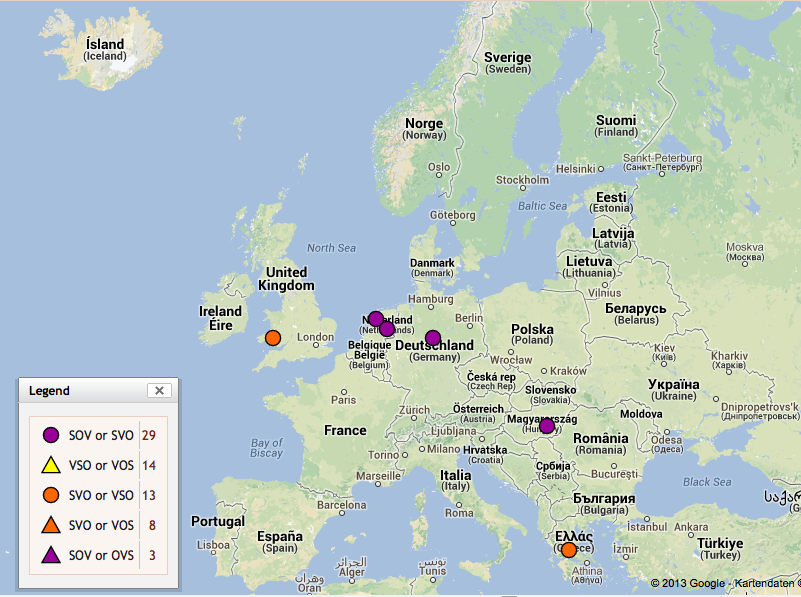
\includegraphics[width=.898\textwidth]{Pictures/WALS-SOV-Europa-no-dominant}
\caption{\label{fig-sov-wals-europe-two}%Dryer: Feature 81b:
Zwei dominante Abfolgen von Subjekt, Objekt und Verb \citep[Abschnitt~3]{Dryer2013c}}
\end{figure}
%% https://wals.info/chapter/81
%% A third subtype of language lacking a dominant order consists of languages in which different word orders occur but the choice is syntactically determined. For example, in \ili{German} and \ili{Dutch}, the dominant order is SVO in main clauses lacking an auxiliary and SOV in subordinate clauses and clauses containing an auxiliary (see below for examples). Because this results in both orders being common, neither order is considered dominant here and these two languages are shown on the map as lacking a dominant word order. In general, if the word order varies according to whether there is an auxiliary verb, the language is shown on the map as lacking a dominant order. Another language whose word order depends both on whether there is an auxigermliary and whether the clause is a main clause is Dinka (Nilotic; Sudan): like \ili{German}, the order is SVO in main clauses without an auxiliary, SAuxOV in main clauses with an auxiliary, but it is VSO in subordinate clauses without an auxiliary and AuxSOV in subordinate clauses with an auxiliary (Nebel 1948: 9, 25, 42, 75, 82).
Der Grund für diese Klassifikation ist, dass \citet[Abschnitt~1]{Dryer2013c} zwischen Sätzen unterscheidet, in denen das finite
Verb das Hauptverb ist (\mex{1}a), und Sätzen, in denen das finite Verb ein Hilfsverb ist wie in (\mex{1}b):
%\largerpage
\eal
\ex
Kim sieht den Fuchs.
\ex
Kim hat den Fuchs gesehen.
\zl
Nach Dryer ist das Muster für (\mex{0}a) SVO und das für (\mex{0}b) SAuxOV, wobei Aux
für Hilfsverb (auxiliary verb) steht. Wie
\citet{Greenberg63a-u}\footnote{%
  Siehe \citew[\page 20--21]{HoehleTopo}.
} zählt Dryer das letztere Muster zur SOV-Abfolge. Die Frage ist, ob man Hilfsverben
bei der Untersuchung der Konstituentenabfolge ignorieren kann. Das Hilfsverb \emph{hat} in (\mex{0}b) verhält sich syntaktisch
wie das Vollverb \emph{scheint} in (\mex{1}):
\ea
Kim scheint den Fuchs zu sehen.
\z
Hier hätten wir also eine SVOV-Abfolge, etwas, das in der diskutierten Typologie nicht existiert.
Die in Abbildung~\ref{fig-sov-wals-europe-two} als nicht über eine dominante Abfolge verfügend markierten Sprachen verwenden die
Verbstellung, um den Satztyp zu markieren: Es ist nur das finite Verb, das in der ersten oder zweiten
Position steht. Nichtfinite Verben stehen final:
\ea
Kim scheint den Fuchs gesehen zu haben.
\z
In Nebensätzen erscheinen sowohl das finite Verb als auch die infiniten Verben in Endstellung, während
das finite Verb in Fragen und deklarativen Hauptsätzen in Initialstellung\footnote{%
  Ich verwende den Begriff Initialstellung, um die Position zu bezeichnen, die das finite Verb in V1- oder V2-Sätzen hat. Die
  Analyse von V2 und V1 beinhaltet die Voranstellung des finiten Verbs. In V2-Sätzen wird zusätzlich
  eine Konstituente vorangestellt.
} steht.
Eine Klassifikation, die ausschließlich auf dem Zählen von Mustern beruht, ohne Hilfsverben und die
Unterscheidung zwischen Finitheit und Nichtfinitheit zu berücksichtigen, kann man diese Stellungstypen nicht auseinanderhalten \citep[Abschnitt~3]{HoehleTopo}. Im Folgenden werden wir uns Haupt- und Nebensätze mit
sowohl finiten als auch infiniten Verben ansehen. Nebensätze offenbaren Unterschiede zwischen OV- und VO-Sprachen, und ich werde argumentieren, dass das \ili{Afrikaans}, das \ili{Niederländisch}e,
das \ili{Deutsch}e und das \ili{Friesisch}e zu den OV-Sprachen gezählt werden sollten und dass das andere beobachtbare Muster
SVO auf andere Eigenschaften dieser Sprachen zurückzuführen ist, nämlich darauf, dass sie den Satztyp durch die Verbstellung
markieren und dass sie Verbzweitsprachen (V2-Sprachen) sind.\footnote{%
  Die Eigenschaft, eine V2-Sprache zu sein, ist unabhängig von der SVO/SOV-Unterscheidung. Alle germanischen\il{Germanisch}
  Sprachen außer dem \ili{Englisch}en sind V2-Sprachen. Siehe Abschnitt~\ref{sec-phenomenon-v2} zu V2.
}

Wenn man komplexere deutsche\il{Deutsch} Sätze mit mehreren Verben bildet, wird das einbettende Verb üblicherweise
rechts von den eingebetteten Verben realisiert.
%\itdopt{M: Are these notions defined somewhere?}
% Yes, in the text immediately following.
Das wird in (\mex{1}) gezeigt. (\mex{1}a) zeigt einen einfachen
Satz mit einem finiten Verb. Wenn wir das Perfekt wie in (\mex{1}b) bilden, muss das Perfekthilfsverb
dem Partizip folgen. Das Hilfsverb ist das finite Verb und es bestimmt die Form des
Partizips. Daher ist das finite Verb das Verb, das das Partizip einbettet. Das wird durch die
niedrigere Nummer von \emph{hat} im Vergleich zu \emph{gesehen} angezeigt. Wenn wir einen noch komplexeren
Satz bilden, indem wir ein weiteres Verb hinzufügen, wird dieses Verb rechts von den vorhandenen Verben angeordnet
(\mex{1}c).  Das dänische\il{Dänisch} Beispiel in (\mex{2}c), das ich leicht angepasst von \citet[\page
146]{Oersnes2009b} übernommen habe, entspricht dem deutschen\il{Deutsch} Beispiel in (\mex{1}c).

\eal
\ex
dass sie ihn sieht$_1$\german
\ex
dass sie ihn gesehen$_2$ hat$_1$
\ex
dass sie ihn gesehen$_3$ haben$_2$ muss$_1$
\zl
\eal
\label{ex-Danish-embedding}
\ex
\gll at   hun ser$_1$ ham\\
     dass sie  sieht    ihn\\\jambox{(\ili{Dänisch})}
\glt `dass sie ihn sieht'
\ex
\gll at   hun have$_1$ set$_2$ ham\\
     dass sie  hat      gesehen ihn\\
\glt `dass sie ihn gesehen hat'
\ex
\gll at   hun må$_1$ have$_2$ set$_3$ ham\\
     dass sie  muss   haben    gesehen ihn\\
\glt `dass sie ihn gesehen haben muss'
\zl
%
Wie die Beispiele in (\mex{0}) zeigen, werden die Verben im \ili{Dänisch}en vor den eingebetteten
Verben hinzugefügt. Das ist auch im \ili{Englisch}en der Fall, das hier zum Dänischen völlig
parallel wäre. Im \ili{Dänisch}en und \ili{Englisch}en gehen die
Verben dem Objekt (\emph{ham}/\emph{him}) voran, und im \ili{Deutsch}en folgen sie ihm
(\emph{ihn}).\footnote{
In deutschen\il{Deutsch} Dialekten gibt es viel Variation, was die Abfolge der Verben angeht, und sogar
das Standarddeutsche\il{Deutsch} erlaubt Abfolgen, in denen einbettende Verben den eingebetteten Verben vorangehen \parencites[\page 63--64]{Bech55a}[\page 180]{dBE83a}:
\ea
weil er nicht wird$_1$ haben$_2$ kommen$_4$ können$_3$
\z
Die Abfolge, in der das einbettende Verb dem eingebetteten Verb vorangeht, ist im \ili{Niederländisch}en Standard \citep[\page 159]{dBE83a}. Kapitel~\ref{chap-verbal-complex}
bietet eine Analyse des Verbalkomplexes in den germanischen\il{Germanisch} OV-Sprachen. Die Verbalkomplexe folgen immer den Objekten.
}

\textcites[\page 15]{Haider2010a}[Abschnitt~15.2]{Haider2020a} weist auf zwei weitere Unterschiede zwischen den germanischen\il{Germanisch} VO- und OV-Sprachen hin:
Partikeln gehen Verben in OV-Sprachen voran \citep[Abschnitt~2.4]{Vikner2001a}, und dasselbe gilt für resultative sekundäre
Prädikate. In VO-Sprachen folgen Partikeln und Resultatprädikate dem Verb. Das wird durch
die folgenden zwei Beispielsätze demonstriert:
%\itdopt{AZ: Kim will look the information up is also possible, footnote?}
\eal
\ex Kim will look up the information.
\ex
Kim wird die Information nachschlagen.\german
\zl
\eal
\ex Kim will fish the pond empty.
\ex
Kim wird den Teich leer fischen.\german
\zl
(\mex{-1}a) zeigt, dass \emph{look} der Partikel \emph{up} vorangeht, während das Verb \emph{schlagen}
im \ili{Deutsch}en der Partikel \emph{nach} folgen muss. Ebenso folgt das sekundäre resultative
Prädikat \emph{empty} dem Verb in (\mex{0}a), aber \emph{leer} geht dem Verb in
(\mex{0}b) voran. Man beachte, dass ich in den Beispielen ein Futurhilfsverb verwendet habe, um Nebeneffekte zu vermeiden, die
auf die Verbzweiteigenschaft des \ili{Deutsch}en zurückzuführen sind: In deklarativen Hauptsätzen geht das finite Verb immer
Partikeln und Resultatprädikaten voran, aber das ist auf den Satztyp zurückzuführen (siehe Abschnitt~\ref{sec-phenomenon-v2}).

%\largerpage[-2]
Ich werde in Kapitel~\ref{chap-verb-position} auf die SVO- vs.\ SOV-Abfolge zurückkommen und mehr von der
Evidenz liefern, die in der Literatur verwendet wurde, um für den OV-Status von Sprachen wie dem \ili{Deutsch}en und dem \ili{Niederländisch}en zu argumentieren.
%\itdopt{M: descriptive OV status is compatible with comparative VO/OV classification.}

Während die germanischen\il{Germanisch} Sprachen sich gut in SOV-Sprachen mit Scrambling (siehe
Abschnitt~\ref{sec-phenomenon-scrambling} weiter unten) und SVO-Sprachen ohne Scrambling aufteilen lassen, gibt es eine
Ausnahme: das \ili{Jiddisch}e. Die folgenden Daten aus \begin{NoHyper}\citew[\page 402]{Diesing97a}\end{NoHyper} zeigen, dass das \ili{Jiddisch}e
die Abfolge haben kann, die üblicherweise in SVO-Sprachen beobachtet wird (\mex{1}a), und die Abfolgen, die in SOV-Sprachen
mit Scrambling beobachtet werden (\mex{1}b, c). Es kann aber auch die Abfolgen in (\mex{1}d) und
(\mex{1}e) haben, in denen das Verb in der Mitte steht und entweder das direkte Objekt oder das indirekte Objekt
dem Verb vorangeht.

\eal
\label{ex-yiddish-vo-ov}
\ex
\gll Maks hot nit gegebn Rifken dos bukh.\\
     Max  hat nicht gegeben  Rifken das Buch\\\yiddish
\glt `Max hat Rifken das Buch nicht gegeben.'
\ex
\gll Maks hot Rifken dos bukh nit gegebn.\\
     Max  hat Rifken das Buch nicht gegeben\\
\glt `Max hat Rifken das Buch nicht gegeben.'
\ex
\gll Maks hot dos bukh Rifken nit gegebn.\\
     Max  hat das Buch Rifken nicht gegeben\\
\glt `Max hat Rifken das Buch nicht gegeben.'
\ex
\gll Maks hot Rifken nit gegebn dos bukh.\\
     Max  hat Rifken nicht gegeben  das Buch\\
\glt `Max hat Rifken das Buch nicht gegeben.'
\ex
\glt Max hat dos bukh nit gegebn Rifken.\\
     Max hat das Buch nicht gegeben  Rifken\\
\glt `Max hat Rifken das Buch nicht gegeben.'
\zl
Es wurde behauptet, das \ili{Jiddisch}e sei eine VO-Sprache
\parencites[\page 113]{dBMvW86a}[\page 388]{Diesing97a}{Sadock98a} oder eine OV-Sprache
\parencites{Hall79a}{Geilfuss90a-u}[Kapitel~2]{Vikner2001a}. Einige Forscher haben argumentiert, dass es
keines von beiden sei: Es wäre ein dritter Sprachtyp, einer mit gemischtem VO/OV-Status \parencites{Santorini93a}[\page 12]{Schallert2007a}[\page 161]{Haider2010a}{Haider2020a}.

%%\largerpage[2]
\citet[Abschnitt~2.5]{Schallert2007a} weist darauf hin, dass viele germanische\il{Germanisch} Sprachen früherer Stufen keine
feste VO- oder OV-Abfolge hatten, und ordnet sie zusammen mit dem \ili{Jiddisch}en dieser dritten Klasse von Sprachen mit
eher freier Verbstellung zu. Seine Klassifikation ist in Tabelle~\ref{table-VO-OV} angegeben.
 
\begin{table}
\oneline{%
\begin{tabular}{llll}\lsptoprule
               & OV-Sprachen                   & VO-Sprachen                   & OV/VO-Sprachen\\\midrule
Nordgermanisch\il{Germanisch} &                                & \ili{Isländisch}, \ili{Färöisch}, & Altnordisch\il{Nordisch!Alt-}, \\
               &                                & \ili{Norwegisch}, \ili{Dänisch}, & (Altisländisch\il{Isländisch!Alt-})\\
               &                                & \ili{Schwedisch}                  &\\
Westgermanisch\il{Germanisch}  & \ili{Deutsch}, \ili{Niederländisch},     & \ili{Englisch}                  & \ili{Jiddisch}, Altenglisch\il{Englisch!Alt-}, \\
               & \ili{Afrikaans}, \ili{Friesisch} &                                & Althochdeutsch\il{Deutsch!Althoch-}, \\
\lspbottomrule
\end{tabular}}
\caption{Konstituentenabfolge-Typologie der germanischen Sprachen nach \citet[\page 13]{Schallert2007a}}\label{table-VO-OV}
\end{table}
\is{Abfolge|)}\is{Abfolge!SVO|)}\is{Abfolge!SOV|)}

\section{V2}
\label{sec-phenomenon-v2}

Die\is{V2-Sprache|(}\is{Abfolge!V2|(} germanischen\il{Germanisch} Sprachen sind, mit Ausnahme des \ili{Englisch}en, sogenannte \emph{Verbzweitsprachen} (V2-Sprachen).
Die V2-Eigenschaft
lässt sich mit den folgenden deutschen\il{Deutsch} Sätzen illustrieren. (\mex{1}) zeigt deklarative Hauptsätze,
in denen eine der Konstituenten vorangestellt ist. (\mex{2}) zeigt parallele Interrogativsätze.

\eal
\ex
Das Kind gibt dem Eichhörnchen jetzt eine Nuss.\german
\ex
Dem Eichhörnchen gibt das Kind jetzt eine Nuss.
\ex
Eine Nuss gibt das Kind dem Eichhörnchen jetzt.
\ex
Jetzt gibt das Kind dem Eichhörnchen eine Nuss.
\zl
\eal
\ex
Wer gibt dem Eichhörnchen jetzt eine Nuss?\german
\ex
Wem gibt das Kind jetzt eine Nuss?
\ex
Was gibt das Kind dem Eichhörnchen jetzt?
\ex
Wann gibt das Kind dem Eichhörnchen eine Nuss?
\zl
Das finite Verb steht in allen Sätzen in (\mex{-1}) und (\mex{0}) in zweiter Position.

Das \ili{Englisch}e hingegen erlaubt keine Abfolgen, in denen das Objekt unmittelbar vor dem
finiten Verb erscheint.

\eal
\ex[*]{
This squirrel give I a nut now.
}
\ex[*]{
This nut give I a squirrel now.
}
\ex[*]{
Tomorrow give I the squirrel a nut.
}
\zl
Adverbiale und Objekte können vorangestellt werden, aber dann müssen sie vor dem Satz erscheinen, der aus
Subjekt und Verb und möglicherweise weiteren Konstituenten besteht.
\eal
\ex This nut, I give the squirrel now.
\ex Now, I give the squirrel a nut.
\zl

\noindent
Man beachte außerdem, dass die Voranstellung von Objekten bei Verben mit zwei Objekten für manche Sprecher auf das sekundäre Objekt
beschränkt ist \citep[\page 258]{Hudson92a-u}.\footnote{
  Ich verwende die Begriffe \emph{primäres Objekt}\is{Objekt!primär} und \emph{sekundäres
    Objekt}\is{Objekt!sekundär} \citep[280]{PS92a}, um die Verwirrung zu vermeiden, die manchmal
  durch die Begriffe \emph{direktes}\is{Objekt!direkt} und \emph{indirektes Objekt}\is{Objekt!indirekt} verursacht wird. Das primäre Objekt ist das erste Objekt im \ili{Englisch}en
  und das Dativobjekt von ditransitiven Verben, die den Dativ regieren, im \ili{Deutsch}en. Das sekundäre Objekt
  ist das zweite Objekt im \ili{Englisch}en und der Akkusativ in deutschen\il{Deutsch} ditransitiven Konstruktionen. Die Abfolge
  Dativ vor Akkusativ ist auch die unmarkierte Abfolge\is{Abfolge!unmarkiert} für die Argumente der meisten ditransitiven Verben
  \citep{Hoehle82a}. Zu Ausnahmen siehe \citew{Cook2006a-u}.
% \ili{Icelandic} dat primary, acc secondary
% \itdopt{M: This is very confusing because the criterion is basically semantic (recipient vs. theme)
%   whereas primary seems to suggest syntactic criteria. It's the same confusion as with
%   direct/indirect.\\
% Stefan: Yes, we are doing syntax.}
} Während also die Voranstellung des sekundären Objekts in
(\mex{1}b) von allen Sprechern erlaubt wird, finden manche Sprecher Extraktionen wie die Extraktion des
primären Objekts in (\mex{1}c) inakzeptabel oder markiert.

\eal
\judgewidth{\%}
\ex[]{
We give children sweets.
}
\ex[]{
These sweets, we give children \_.
}
\ex[\%]{
These children, we give \_ sweets.
}
\zl
In V2-Sprachen ist das nicht der Fall: Sie sind, was die Voranstellung angeht, recht
liberal. Im Prinzip können alle Konstituenten vorangestellt werden, mit Ausnahme von Reflexiv\-pronomen,
die von inhärent reflexiven Verben\is{Verb!inhärent reflexiv} selegiert werden (\mex{1}), expletiven\is{Pronomen!expletiv} Objekten (\mex{2}) und bestimmten Modal\-partikeln (\mex{3}). Siehe auch \citew[\page 159]{Hoberg81a} zu inhärent reflexiven
Verben\is{Verb!inhärent reflexiv} und Modalpartikeln.
\eal
\ex[]{
Maria erholt sich.\german
}
\ex[*]{
Sich erholt Maria.
}
\zl
\eal
\ex[]{
Er bringt es bis zum Professor.\german
}
\ex[\#]{
Es bringt er bis zum Professor.
}
\zl
\eal
\ex[]{
Er geht halt nicht.\german
}
\ex[*]{
Halt geht er nicht.
}
\zl
%\itdopt{AZ: why do you call es an EXPL in this case? it seems to be a pronominal object}
Das Element vor dem finiten Verb ist nicht notwendigerweise ein Satzgenosse des finiten Verbs. Tatsächlich
kann es zu einem tief eingebetteten Kopf gehören, wie das folgende Beispiel aus dem
\ili{Deutsch}en zeigt:
\ea
{}[Über dieses Thema]$_i$ habe ich sie gebeten, [[einen Vortrag \_$_i$~] zu halten].\footnote{
Adaptiert nach \citew[\page 21]{HN89b}.
}\german

\z
Die PP \emph{über dieses Thema} hängt von dem Nomen \emph{Vortrag} ab, das Teil der VP ist, deren Kopf
\emph{zu halten} ist. Diese VP ist unter \emph{gebeten} eingebettet. Sätze wie
(\mex{0}) zeigen, dass V2-Voranstellungen nicht als eine einfache Umstellung der Argumente eines
Verbs analysiert werden können. Während ein solcher Ansatz für die Beispiele in (\mex{1}) funktionieren würde, ließe er sich nicht auf andere
Fälle übertragen, in denen das vorangestellte Element nicht vom höchsten Verb im Satz abhängt.
\ea
Den Text kennt er.
\z

\noindent
Die folgenden Beispiele aus dem \ili{Dänisch}en (SVO) zeigen, dass die Eigenschaft, eine V2-Sprache
zu sein, unabhängig von der VO/OV-Eigenschaft ist:
\eal
\ex
\gll Gert har læst bogen.\\
     Gert hat gelesen Buch.\textsc{def}\\\danish
\glt `Gert hat das Buch gelesen.'
\ex
\gll Bogen har Gert læst.\\
     Buch.\textsc{def} hat Gert gelesen\\
\glt `Gert hat das Buch gelesen.'
\zl
Das Beispiel in (\mex{0}a) zeigt, dass das Objekt den Verben folgt, und (\mex{0}b) zeigt, dass das
Objekt \emph{bogen} in Satzanfangsstellung vor dem finiten Verb
\emph{har} erscheinen kann.

Die V2-Abfolge wird in den germanischen\il{Germanisch} Sprachen (außer dem \ili{Englisch}en) durchgängig in deklarativen Hauptsätzen verwendet.
Einige germanische\il{Germanisch} Sprachen erlauben die V2-Abfolge nicht in eingebetteten Sätzen. Für eine Diskussion
eingebetteter Interrogativsätze siehe Abschnitt~\ref{sec-embeeded-clauses}.

Während das \ili{Englisch}e die Abfolge Objekt"=Verb"=Subjekt nicht erlaubt, die in den anderen germanischen\il{Germanisch}
Sprachen aufgrund der V2-Voranstellung möglich ist, erlaubt es die Voranstellung des Objekts in Fragen, was zu
Strukturen führt, die parallel zu dem sind, was wir aus den anderen germanischen\il{Germanisch} Sprachen kennen:
\eal
\ex\label{ex-which-book-did-sandy-read}
Which book did Sandy read?
\ex\label{ex-which-book-did-sandy-give-to-kim}
Which book did Sandy give to Kim?
\ex To whom did Sandy give the book?
\zl
Das \ili{Englisch}e war früher eine V2-Sprache, hat diese Eigenschaft aber verloren. Das V2 in Fragen ist ein Überbleibsel früherer
Sprachstufen, weshalb das \ili{Englisch}e eine \emph{residuale V2-Sprache}\is{V2-Sprache!residual} genannt wird \citep[\page 375]{Rizzi1990a-u}.

V2 und Verbvoranstellung allgemein sind eine Möglichkeit, Satztypen in allen germanischen\il{Germanisch} Sprachen zu markieren. V2-Sätze
können in allen germanischen\il{Germanisch} Sprachen außer dem \ili{Englisch}en deklarative Sätze sein, und sie können in allen
germanischen\il{Germanisch} Sprachen einschließlich des \ili{Englisch}en Fragen sein. Außerdem können V2-Sätze Imperative sein, wie (\mex{1}) zeigt.
\ea
Jetzt gib ihr das Buch!
\z
Sätze mit dem finiten Verb in erster Position (V1) können Ja/Nein-Fragen oder Imperative sein:
\eal
\ex
Gibt er ihr das Buch?
\ex
Gib ihr das Buch!
\zl
Natürlich ist die Abfolge der Elemente nicht der einzige Hinweis auf den vorliegenden Satztyp. Auch Intonation und morphologische Markierung von Imperativformen spielen eine Rolle.

Die Eigenschaft, eine V2-Sprache zu sein, ist unter den Sprachen der Welt überaus selten \citep[\page
  343]{Holmberg2015a}. Abgesehen von den germanischen\il{Germanisch} Sprachen mit Ausnahme des
modernen \ili{Englisch}en \citep{HP86a-ed} sind die einzigen bekannten Fälle das \ili{Estnisch}e (Finno-Ugrisch, \citealp[\page 343]{Holmberg2015a}), das \ili{Sorbisch}e \citep[Eintrag~79]{Plank2003b-ed} (eine slawische\il{Slawisch} Sprache), die
keltischen\il{Keltisch} Sprachen \ili{Bretonisch} \citep{BK2000a-u}, \ili{Kornisch} \citep*[\page 287]{BTW2007a-u} und
Mittelwalisisch\il{Walisisch!Mittel} \citep{Willis1998a-u}, Altfranzösisch\il{Französisch!Alt-} \parencites[Abschnitt~1.3]{Adams1987a-u}[Abschnitt~2.1.2]{Roberts93a-u}[Kapitel~2]{Vance97a-u}, Altspanisch\il{Spanisch!Alt}
% Plank2003b-ed: and some other early \ili{Romance} languages
%\citep{Fontana93a,Fontana97a},
\citep[Abschnitt~3.3.2]{Fontana97a-u},
\ili{Rätoromanisch} \citep{Poletto2002a-u,Anderson2006a-u}, Kaschmiri
\citep[Kapitel~4]{Bhatt99a-u}, zwei Dialekte des \ili{Himachali}, das ebenfalls zum \ili{Indoarisch}en gehört
und in an Kaschmiri angrenzenden Regionen gesprochen wird \citep{Hendriksen90a}, die austronesischen\il{Austronesisch}
Sprachen \ili{Taiof} und \ili{Sisiqa} \citep[\page 495]{Ross2004a-u} und die brasilianische indigene
Sprache \ili{Karitiana} aus der Tupí-Sprachfamilie \citep{Storto2003a-u}.
% This is mentioned in Bayer2010, but maybe it is like the australian languages.
% and the
%Uto-Aztekian language \ili{Tohono O'odham}, which is spoken in the southwest of the US and in northern Mexico.
% Estnisch 
\is{V2-Sprache|)}\is{Abfolge!V2|)}

\section{Scrambling}
\label{sec-phenomenon-scrambling}

Während\is{Scrambling|(} die Konstituentenabfolge in Sprachen wie dem \ili{Englisch}en eher festgelegt ist, erlauben Sprachen wie das \ili{Niederländisch}e und
das \ili{Deutsch}e eine freiere Permutation der Argumente. Um die Effekte nicht durch
Umstellungen zu verfälschen, die auf die V2-Eigenschaft zurückzuführen sind, verwende ich Verbletztsätze, um das
Phänomen im \ili{Deutsch}en zu illustrieren. Beispiel (\mex{1}) zeigt die einzige mögliche Abfolge von Subjekt und Objekten eines einfachen
ditransitiven Satzes im \ili{Englisch}en ohne Extraktion:

\ea
because the child gives the squirrel the nut \english
\z
Wenn Sprecher das sekundäre Objekt \emph{the nut} vor dem primären Objekt \emph{the
  squirrel} realisieren wollen, müssen sie ein Präpositionalobjekt verwenden. Diese Art der Umstellung wird
\emph{Dative Shift} genannt, und (\mex{1}) ist ein Beispiel:
\ea
because the child gives the nut to the squirrel \english
\z
Im Gegensatz dazu haben wir die deutschen\il{Deutsch} Beispiele in (\mex{1}). Diese Beispiele zeigen, dass die Nominal\-phrasen
frei permutiert werden können:
\eal
\ex
{}[weil] das Kind dem Eichhörnchen die Nuss gibt\german
\ex
{}[weil] das Kind die Nuss dem Eichhörnchen gibt
\ex
{}[weil] die Nuss das Kind dem Eichhörnchen gibt
\ex
{}[weil] die Nuss dem Eichhörnchen das Kind gibt
\ex
{}[weil] dem Eichhörnchen das Kind die Nuss gibt
\ex
{}[weil] dem Eichhörnchen die Nuss das Kind gibt
\zl
Nicht alle dieser Abfolgen können in allen Kontexten verwendet werden. Einige der Beispiele erfordern eine besondere,
kontrastive Intonation. Die Abfolgen können nach der Anzahl der Kontexte sortiert werden, in denen
sie verwendet werden können. \citet{Hoehle82a} schlägt vor, die Abfolge, die in den meisten Kontexten verwendet werden kann, die
normale oder unmarkierte Abfolge\is{Abfolge!unmarkiert} zu nennen.

Die OV-Sprachen teilen viele Eigenschaften, sodass man erwarten würde, dass das \ili{Niederländisch}e ebenfalls Scrambling
erlaubt. Objekt-NPs können jedoch nicht gescrambelt werden:
\ea[*]{
\longexampleandlanguage{
\gll Toen hebben de  autoriteiten het kind de moeder  teruggegeven\\
     dann haben   die Behörden  das Kind die Mutter  zurückgegeben\\}{Niederländisch}
\glt Intendiert: `Die Behörden gaben das Kind der Mutter zurück.'
}
\z
Der Grund dafür ist, dass NPs im \ili{Niederländisch}en nicht kasusmarkiert sind. Es wäre für Hörer
und Leser sehr schwierig herauszufinden, wer wem was angetan hat. Das ist parallel zu Beispielen mit kasuslosen NPs im
\ili{Deutsch}en. Wie \citet[\page 45]{Wegener85b} feststellt, ist (\mex{1}) nicht mehrdeutig:
\ea
\label{ex-sie-mischt-dem-wein-wasser-bei}
Sie mischt Wein Wasser bei.
\z
Das bedeutet, dass es Wein gibt und Wasser hinzugefügt wird. Das entspricht der Abfolge dat < akk.
Die Situation ist mit Determinatoren anders:
\eal
\ex
Sie mischt dem Wein das Wasser bei.
\ex
Sie mischt das Wasser dem Wein bei.
\zl
Mit Determinatoren erhalten wir die Lesart in (\mex{-1}) unabhängig von der Abfolge der Nominalphrasen. Wenn
wir die Abfolge der determinatorlosen NPs in (\mex{-1}) ändern, erhalten wir dagegen eine andere Lesart:
\ea
Sie mischt Wasser Wein bei.
\z
Ohne jegliche Hinweise aus der Kasusmarkierung (oder dem Kontext oder der Intonation) hat man also die Abfolge dat < akk; mit
Kasusmarkierung sind beide Abfolgen möglich.
%
% Tibor 2025: Siehe etwa (ich habe das mit Simon Masloch und der wiederum mit Sarah Broll (IDS) diskutiert und das Bsp. ist von ihnen):
%
%(1) Welchem Getränk mischt Sabine Wasser bei?
%(2) Sie mischt Wasser Wein bei.
%
% in der ganzen Debatte habe ich noch vergessen, ein Beispiel nachzureichen, das unser Glossa-Papier sozusagen fortsetzt (auf das mich ebenfalls SM und SB noch aufmerksam gemacht haben):
%
% (1) Jeder weiß, dass Yoko Ono John Lennon gefällt.
%
% Hier hat man keinerlei Kasus-Markierung und dennoch kein „Freezing“ oder wie man es nennen will. Wir führen das darauf zurück, dass Beispiele mit _gefallen_ und zwei belebten Argumenten keine Abfolgepräferenzen besitzen, also in der Realisation echt optional sind (was natürlich unter der Annahme einer Basisabfolge kaum erklärbar ist).

Um auf das \ili{Niederländisch}e zurückzukommen: Die Beispiele in (\mex{1}) zeigen, dass Scrambling tatsächlich möglich ist, wenn die Argumente
identifiziert werden können \parencites[\page 989]{GHdRvdT1984a-ed}[\page 14, 152]{Haider2010a}:
\eal
\ex
\longexampleandlanguage{
\gll Toen hebben de autoriteiten het kind  aan de  moeder teruggegeven.\\
     dann haben   die Behörden das Kind  an  die Mutter zurückgegeben\\}{Niederländisch}
\glt `Dann haben die Behörden das Kind der Mutter zurückgegeben.'
\ex
\gll Toen hebben de  autoriteiten aan de moeder  het kind  teruggegeven\\
     dann haben   die Behörden  an  die Mutter  das Kind  zurückgegeben\\
\glt `Dann haben die Behörden das Kind der Mutter zurückgegeben.'
\zl
(\mex{0}) enthält Beispiele mit NP- und PP-Objekt. Da die PP klar identifizierbar ist, können die beiden
Argumente in beliebiger Abfolge erscheinen. Es scheint daher gerechtfertigt anzunehmen, dass die OV-Sprachen (das \ili{Deutsch}e,
das \ili{Niederländisch}e, das \ili{Afrikaans}, das \ili{Friesisch}e) Scrambling erlauben, mit Beschränkungen, die das Scrambling von Elementen verbieten, die
nicht identifizierbar sind.%
\is{Scrambling|)}

\section{Die Stellung von Adverbialen}
\label{sec-phenomena-position-of-adverbials}

In\is{Abfolge!Adverbiale|(} Sprachen wie dem \ili{Deutsch}en und dem \ili{Niederländisch}en ist die Stellung von Adverbialen recht frei: das Adverb \emph{gestern}
kann überall zwischen den Argumenten und dem Verb erscheinen:
\eal
\ex
weil das Kind dem Eichhörnchen die Nuss \emph{gestern} gab
\ex
weil das Kind dem Eichhörnchen \emph{gestern} die Nuss gab
\ex
weil das Kind \emph{gestern} dem Eichhörnchen die Nuss gab
\ex
weil \emph{gestern} das Kind dem Eichhörnchen die Nuss gab
\zl
Auch das \ili{Niederländisch}e hat eine freie Abfolge von Adverbialen \parencites[\page 387]{Neeleman94b-u}[\page
4]{Koster99a-u}[Abschnitt~6]{Bouma2003a-u}. (\mex{1}) zeigt die niederländischen\il{Niederländisch} Beispiele, die
(\mex{0}) entsprechen:
% Neeleman sagt, das sei base-Generation.
% Bouma2003a:6
% \eal
% \ex
% \gll dat  Kim regelmatig haar moeder bezoekt\\
%      that Kim regularly  her  mother visits\\\dutch
% \glt `that Kim visit her mother regularly'
% \ex
% \gll dat  Kim haar moeder regelmatig bezoekt\\
%      that Kim her  mother regularly  visits\\
% \glt `that Kim visit her mother regularly'
% \zl
\eal
\ex
\gll omdat het kind de eekhoorn de noot \emph{gisteren} gaf\\
     weil das Kind das Eichhörnchen die Nuss gestern gab\\\dutchshort
\glt `weil das Kind dem Eichhörnchen die Nuss gestern gab'
\ex
\gll omdat het kind de eekhoorn \emph{gisteren} de noot gaf\\
     weil das Kind das Eichhörnchen gestern die Nuss gab\\
\ex
\gll omdat het kind \emph{gisteren} de eekhoorn de noot gaf\\
     weil das Kind gestern das Eichhörnchen die Nuss gab\\
\ex
\gll omdat \emph{gisteren} het kind de eekhoorn de noot gaf\\
     weil gestern das Kind das Eichhörnchen die Nuss gab\\
\zl

\noindent
Im Gegensatz dazu ist die Stellung der Adverbiale in SVO-Sprachen wie dem \ili{Dänisch}en und dem
\ili{Englisch}en eher eingeschränkt. Die Adverbiale werden üblicherweise vor oder nach der VP platziert; das heißt, Verb und Objekte bilden eine
Einheit, und Adverbiale schließen sich links oder rechts an diese Einheit an. (\mex{1}) liefert ein Beispiel:
\eal
\ex[]{
because the child {often} [gave the squirrel the nut] \english
}
\ex[]{
because the child [gave the squirrel the nut] {often}
}
\ex[*]{
because the child [gave often the squirrel the nut]
}
\ex[*]{
because the child [gave the squirrel often the nut]
}
\zl
Es wird angenommen, dass Verb und Objekte in diesen Sprachen eine strukturelle Einheit bilden, eine Verbalphrase (VP). Adverbiale können
sich an diese VP anschließen und eine größere VP bilden, die dann mit dem Subjekt zu einem vollständigen Satz kombiniert wird.

Das folgende Beispiel, das auf \citet[§ 8.20, 495]{QGLS85a-u} zurückgeht, zeigt, dass selbst in sehr
komplexen Kombinationen mehrerer Verben Adverbien an der linken Peripherie einer VP platziert werden können:
\ea
It [certainly [\sub{VP} may [possibly [\sub{VP} have [indeed\\ \hfill{}[\sub{VP} been {}[badly [\sub{VP} formulated]]]]]]]].
\z
Für das Englische scheinen also Verben und Objekte eine Einheit zu bilden. Ketten von einander
einbettenden Verben ohne die zugehörigen nicht-verbalen Argumente sind nicht möglich.
Das ist anders als in den OV-Sprachen, wo Verben einen Verbalkomplex bilden, der normalerweise nicht
durch Adverbien unterbrochen werden kann. So kann das Adverb \emph{morgen} in den Beispielen in
(\mex{1}) nicht zwischen den Verben stehen:
\eal
\ex[]{
dass das Kind dem Eichhörnchen die Nuss morgen geben dürfen muss
}
\ex[*]{
dass das Kind dem Eichhörnchen die Nuss geben morgen dürfen muss
}
\ex[*]{
dass das Kind dem Eichhörnchen die Nuss geben dürfen morgen muss
}
\zl
\is{Abfolge!Adverbiale|)}

\section{Eingebettete Sätze}
\label{sec-embeeded-clauses}

Dieser Abschnitt befasst sich mit eingebetteten Sätzen, die durch einen Komplementierer eingeleitet werden, und mit
eingebetteten Interrogativsätzen. Die germanischen\il{Germanisch} Sprachen variieren hinsichtlich der Verbstellung in
diesen Nebensätzen und hinsichtlich der Frage, ob die eingebetteten Sätze V2 sind oder nicht.

\subsection{Durch einen Komplementierer eingeleitete eingebettete Sätze}

Wie bereits erwähnt, sind das \ili{Afrikaans}, das \ili{Niederländisch}e und das \ili{Deutsch}e SOV-Sprachen, und das zeigt sich in eingebetteten
Sätzen, die durch einen Komplementierer eingeleitet werden. (\mex{1}) ist ein Beispiel:

\ea
Ich weiß, dass Aicke das Buch heute gelesen hat.
\z
%%
%% Stellung der anderen Konstituenten ist frei:
%% \eal
%% \ex Ich weiß, dass das Buch Max heute gelesen hat.
%% \ex Ich weiß, dass das Buch heute Max gelesen hat.
%% \zl

\noindent
Das \ili{Englisch}e, das eine SVO-Nicht-V2-Sprache ist, erlaubt nur die SVO-Abfolge.
\ea{
I  know that Kim read the book yesterday. \english
}
\z

\noindent
Interessanterweise erlaubt das \ili{Dänisch}e, ebenfalls eine SVO-Sprache, in Sätzen, denen ein Komplementierer vorausgeht, sowohl die SVO-Abfolge (\mex{1}) als auch die V2-Abfolge (\mex{2}):
\ea[]{
\label{ex-at-max-ikke-har}
\gll Jeg  ved, at   Gert ikke  har læst   bogen          {i dag}.\\
     ich weiß dass Gert nicht hat gelesen Buch.\textsc{def} heute\\\jambox{(\ili{Dänisch})}
\glt `Ich weiß, dass Gert das Buch heute nicht gelesen hat.'
}
\z
%(Negation hilft, Verbstellung zu bestimmen)

\eal
\ex{
\gll Jeg  ved, at   {i dag} har Gert ikke læst bogen.\\
     ich weiß dass heute   hat Gert nicht gelesen Buch.\textsc{def}\\\jambox{(\ili{Dänisch})}
}
\ex{
\gll Jeg  ved, at   bogen          har Gert ikke  læst {i dag}.\\
     ich weiß dass Buch.\textsc{def} hat Gert nicht gelesen heute\\
}
\zl
Das Beispiel in (\ref{ex-at-max-ikke-har}) enthält eine Negation, um zu zeigen, dass wir es hier tatsächlich
mit einer SVO-Abfolge zu tun haben. Ohne die Negation wäre nicht klar, ob Nicht-V2-Sätze in
Sätzen erlaubt sind, die durch einen Komplementierer eingeleitet werden, da in (\mex{1}a) das finite Verb an zweiter
Stelle steht. Bei vorhandener Negation ist klar, dass wir einen V2-Satz haben, wenn die Negation dem
finiten Verb folgt, und dass wir keinen V2-Satz haben, wenn das finite Verb nach der Negation und
somit in dritter Position steht wie in (\mex{-1}).
\eal
\settowidth\jamwidth{(V2 or SVO)}
\ex
\gll at Gert har læst bogen\\
     dass Gert hat gelesen Buch.\textsc{def}\\\jambox{(V2 or SVO)}
\ex
\gll at Gert har ikke læst bogen\\
     dass Gert hat nicht gelesen Buch.\textsc{def}\\\jambox{(V2)}
\zl
Für komplementiererlose Sätze ist die V2-Abfolge die einzig mögliche:
\eal
\settowidth\jamwidth{(V2 or SVO)}
\ex[]{
\gll Gert har ikke læst bogen\\
     Gert hat nicht gelesen Buch.\textsc{def}\\\jambox{(V2)}
}
\ex[*]{
\gll Gert ikke har læst bogen\\
     Gert nicht  hat gelesen Buch.\textsc{def}\\\jambox{(SVO)}
}
\zl

\noindent
Das \ili{Jiddisch}e und das \ili{Isländisch}e sind ebenfalls SVO-Sprachen. Die Sätze, die mit einem
Komplementierer kombiniert werden, sind V2:
\eal
\ex
\gll Ikh meyn  az   haynt hot Max geleyent dos bukh.\footnotemark\\
     ich denke dass heute hat Max gelesen das Buch\\\yiddish
\footnotetext{\citew[\page 58]{Diesing90a}}
\glt `Ich denke, dass Max das Buch heute gelesen hat.'

\ex% check!
\gll Ikh meyn  az   dos bukh hot Max geleyent.\\
     ich denke dass das Buch hat Max gelesen\\

\zl
\ea
\longexampleandlanguage{
\gll Engum         datt í hug,  að   vert  væri að reyna til     að kynnast honum.\footnotemark\\
     niemand.\DAT{} fiel zu Sinn dass wert war  zu versuchen \PREP{} zu kennenlernen ihn\\}{Isländisch}
\footnotetext{\citew[\page 75]{Maling90a-u}}
\glt `Es kam niemandem in den Sinn, dass es sich lohnte zu versuchen, ihn kennenzulernen.'
\z
% Haider2010a:47 \ili{Frisian} as well
%a. Ik leau [dat hy him wol rêde kin] \ili{Frisian} 
%   I think [that he him well save can]
%b. Ik leau [dat hy kin him wol rêde] c. Ik leau [hy kin him wol rêde]

\subsection{Interrogativnebensätze}

Die OV-Sprachen bilden untergeordnete Interrogativsätze, indem sie eine Phrase, die ein
Interrogativpronomen enthält\footnote{
Die meisten Interrogativpronomen beginnen im \ili{Deutsch}en mit \emph{w} und im \ili{Englisch}en mit \emph{wh}. Phrasen,
die ein Interrogativpronomen enthalten, werden \emph{w}"=Phrasen bzw.\ \emph{wh}"=Phrasen
genannt. Interrogativsätze werden manchmal \emph{w}"=Sätze oder \emph{wh}"=Sätze genannt.
}, aus einem
ansonsten SOV-Satz voranstellen. (\mex{1}) zeigt ein deutsches\il{Deutsch} Beispiel:
\eal
\ex
Ich weiß, wer heute das Buch gelesen hat.\german
\ex
Ich weiß, was Aicke heute gelesen hat.
\zl
Da Sprachen wie das \ili{Deutsch}e Scrambling erlauben, könnten Sätze wie die in (\mex{0}) einfach auf
die Permutation der Argumente eines Kopfes zurückzuführen sein. Die Generalisierung über diese \emph{w}"=Sätze
ist jedoch, dass ein beliebiges \emph{w}"=Element vorangestellt werden kann. (\mex{1}) gibt ein Beispiel aus dem \ili{Deutsch}en, das
eine Fernabhängigkeit beinhaltet:
\ea
Ich weiß nicht, [über welches Thema]$_i$ sie versprochen hat,\\ \hfill{}[[einen Vortrag \_$_i$] zu halten].\german
\z
Hier ist die Phrase \emph{über welches Thema} ein Argument des Nomens \emph{Vortrag},
das in der VP eingebettet ist, die \emph{zu halten} enthält. Die \emph{zu halten}"=VP ist unter
\emph{versprochen hat} eingebettet. Die Generalisierung über Interrogativnebensätze ist, dass ein
Interrogativsatz aus einer Interrogativphrase (\emph{über welches Thema})
und einem Satz besteht, in dem diese Interrogativphrase irgendwo fehlt (\emph{er versprochen
  hat, einen Vortrag zu halten}).

Im \ili{Deutsch}en ist die Abfolge der anderen Konstituenten frei wie in den zuvor diskutierten assertiven Hauptsätzen und eingebetteten
Sätzen mit einem Komplementierer.
\eal
\ex
Ich weiß, was keiner diesem Eichhörnchen geben würde.\german
\ex
Ich weiß, was diesem Eichhörnchen keiner geben würde.
\zl

\noindent
Im \ili{Dänisch}en und \ili{Englisch}en bestehen die Interrogativsätze aus einer Interrogativphrase und einem SVO-Satz,
in dem sie fehlt:
\eal
\ex
\gll Gert har givet ham bogen.\\
     Gert hat gegeben ihm Buch.\textsc{def}\\\jambox{(\ili{Dänisch})}
\glt `Gert hat ihm das Buch gegeben.'
\ex
\gll Jeg ved, hvad$_i$ [Gert har givet ham \_$_i$].\\
     ich weiß was \spacebr{}Gert hat gegeben ihm\\
\glt `Ich weiß, was Gert ihm gegeben hat.'
\ex
\gll Jeg ved, hvem$_i$ [Gert har givet \_$_i$   bogen].\\
     ich weiß wem        \spacebr{}Gert hat gegeben {} Buch.\textsc{def}\\
\glt `Ich weiß, wem Gert das Buch gegeben hat.'
\zl
(\mex{0}a) zeigt den Satz mit SVO-Abfolge, (\mex{0}b) ist ein Beispiel mit dem sekundären Objekt als
Interrogativpronomen und (\mex{0}c) ist ein Beispiel mit dem primären Objekt als
Interrogativpronomen. Die Position, die die jeweiligen Objekte in nicht-interrogativen Sätzen wie (\mex{0}a)
haben, ist mit \_$_i$ markiert.

Das \ili{Jiddisch}e ist insofern besonders, als es auch in Interrogativsätzen die V2-Abfolge hat \citep[Abschnitte~4.1, 4.2]{Diesing90a}: Interrogative
bestehen aus einer Interrogativphrase, die aus einem V2-Satz extrahiert ist:

\ea
\gll Ir veyst efsher [avu            do    voynt Roznblat   der goldshmid]?\footnotemark\\
     du weißt vielleicht  \spacebr{}wo  da   wohnt Roznblat der Goldschmied\\
\glt `Weißt du vielleicht, wo Roznblat der Goldschmied wohnt?'
% The gollsing an translation differes in the original Rozenblatt
\footnotetext{
\citew[\page 65]{Diesing90a}. Zitiert aus Olsvanger, \emph{Royte Pomerantsn}, 1949.
}
\z
%
%% \eal 
%% \ex
%% \label{vosmaks}
%% \gll Ikh veys nit   vos$_i$ [Max hot gegesn \_$_i$].\footnotemark\\
%%      I know not     what \hphantom{[}Max has eaten\\
%% \footnotetext{\citew[\page 68]{Diesing90a}.}
%% \glt `I do not know what Max has eaten.'
%%
%% \ex%check
%% \gll Ikh veys nit   [vos                    hot Max gegesn].\footnotemark\\
%%      ich weiß nicht \hphantom{[}was heute hat Max gegessen\\
%% \footnotetext{\citew[S.\,68]{Diesing90a}.}
%% \glt `Ich weiß nicht, was Max heute gegessen hat.'
%\zl
\noindent
Die Variation, die wir unter den germanischen\il{Germanisch} Sprachen finden, ist also \emph{w}-Phrase + SOV, \emph{w}-Phrase + SVO und \emph{w}-Phrase + V2.

\section{Die Verwendung von Expletiva zur Markierung des Satztyps}

Die germanischen\il{Germanisch} Sprachen verwenden die Konstituentenabfolge, um den Satztyp zu kodieren: V2-Hauptsätze können
Aussagen oder Fragen sein, abhängig vom Inhalt des Materials vor dem Verb und der
Intonation. Ebenso bestehen eingebettete Interrogativsätze aus einer \emph{w}"=Phrase und einem SVO-, SOV-
oder V2-Satz. Die Voranstellung einer Konstituente in einem V2-Satz geht mit bestimmten informationsstrukturellen
Effekten einher: Etwas ist das Topik oder der Fokus einer Äußerung. Für eingebettete Sätze ist es
für manche Sprachen wichtig, dass die Struktur transparent ist, d.h.\ dass wir die Abfolge \emph{w} + SVO oder
\emph{w} + V2 haben. Es gibt Situationen, in denen es unangemessen ist, ein Element voranzustellen, und in
solchen Situationen verwenden die germanischen\il{Germanisch} Sprachen Expletiva, das heißt Pronomen, die nichts
semantisch beitragen, um eine bestimmte Abfolge aufrechtzuerhalten.

Das \ili{Deutsch}e verwendet das Expletivum\is{Pronomen!expletiv} \emph{es}, um die Position vor dem finiten Verb zu füllen, wenn keine andere
Konstituente vorangestellt werden soll.
\eal
\ex
Drei Reiter ritten zum Tor hinaus.\german
\ex
Es ritten drei Reiter zum Tor hinaus.
\zl

%\largerpage
\noindent
Das \ili{Dänisch}e verwendet das Expletivum\is{Pronomen!expletiv}, um deutlich zu machen, dass eine Extraktion einer Konstituente stattgefunden hat
%\itdopt{AZ: this assumes a lot of analysis that has not been provided yet. Maybe rephrase: \ili{Danish} uses an expletive in sentences such as ... In Chapter ?? we will show that the language here avoids string vacuous movement.}
% St.Mü: This is explained below the sentence.
\citep[\page 169]{MOe2011a}:\footnote{
  Mit DK markierte Beispiele stammen aus KorpusDK, einem Korpus von 56 Millionen Wörtern, das das
  zeitgenössische \ili{Dänisch} dokumentiert (\url{http://ordnet.dk/korpusdk}).
}
\eal
\ex[]{
\longexampleandlanguage{
\gll Politiet            ved   ikke,  hvem der           havde placeret bomben.\footnotemark\\
     Polizei.\textsc{def} weiß nicht    wer  \textsc{expl} hat platziert Bombe.\textsc{def}\\}{Dänisch}
\footnotetext{DK}
\glt `Die Polizei weiß nicht, wer die Bombe platziert hat.'
}
\ex[*]{
\gll Politiet ved ikke,  hvem havde placeret bomben.\\
     Polizei.\textsc{def} weiß nicht wer hat platziert Bombe.\textsc{def}\\
}
\zl
Ohne das Expletivum\is{Pronomen!expletiv} ergäbe sich die Abfolge in (\mex{0}b). In (\mex{0}b) haben wir die
normale SVO-Abfolge, und es ist für die Hörer*in nicht offensichtlich, dass der Satz aus einem extrahierten
Element (dem Subjekt) und einem SVO-Satz besteht, in dem es fehlt. Das ist transparenter, wenn ein
Expletivum in die Subjektposition eingefügt wird wie in (\mex{0}a). (\mex{1}) zeigt das anhand der
Analyse, die in Kapitel~\ref{chap-expletives} vorgeschlagen wird: (\mex{1}a) zeigt die hypothetische
Struktur, die sich ergeben würde, wenn man annähme, dass das Subjekt \emph{hvem} `wer'
extrahiert ist. Es würde sich ein sogenanntes \emph{string vacuous movement} ergeben: Das Subjekt wird an einen Platz
direkt neben dem Satz, aus dem es kommt, bewegt, so dass die Bewegung nicht sichtbar ist. In (\mex{1}b) hingegen wird die Subjektposition vom Expletivum eingenommen, und
daher ist klar, dass der eingebettete Satz eine besondere Struktur hat. Es gibt eine sichtbare Markierung für
die Hörer*in oder Leser*in des Satzes, die ihn als eingebetteten Interrogativsatz kennzeichnet.
\eal
\ex[*]{
\gll [hvem$_i$     [\trace$_i$ havde placeret bomben]]\\
     \spacebr{}wer {}          hat platziert Bombe.\textsc{def}\\\danish
}
\ex[]{
\gll [hvem$_i$     [der                    havde \trace$_i$ placeret bomben]]\\
     \spacebr{}wer \spacebr{}\textsc{expl} hat   {}         platziert Bombe.\textsc{def}\\
}
\zl

%\largerpage
\noindent
Ebenso verwendet das \ili{Jiddisch}e ein Expletivum\is{Pronomen!expletiv} in eingebetteten Interrogativen (\emph{w} + V2), wenn
%the subject is extracted and
es kein anderes Element gibt, das informationsstrukturell für die präverbale Position geeignet ist.
%% \ea
%% \label{vosmaks}
%% \gll Ikh veys nit   [vos Max hot gegesn].\footnotemark\\
%%      ich weiß nicht \hphantom{[}was Max hat gegessen\\
%% \footnotetext{\citew[S.\,68]{Diesing90a}.}
%% \glt `Ich weiß nicht, was Max gegessen hat.'
%% \z
%% 
%% \item 
(\mex{1}) zeigt Beispiele aus \citet[\page 403--404]{Prince89a}:

\eal
\ex[]{
\gll ikh hob  zi  gefregt ver es         iz beser  far ir\\
     ich habe sie gefragt wer \textsc{expl} ist besser für sie\\\yiddish
\glt `Ich habe sie gefragt, wer besser für sie ist.'}
\ex[]{
\gll ikh hob  im  gefregt vemen es        kenen ale dayne khaverim\\
     ich habe ihn gefragt wen \textsc{expl} kennen alle deine Freunde\\
\glt `Ich habe ihn gefragt, wen alle deine Freunde kennen.'}
\zl
(\mex{0}a) ist ein Beispiel mit einem Interrogativpronomen, das das Subjekt ist, und (\mex{0}b) ist ein
Beispiel, in dem die präverbale Position nicht von einem Argument von \emph{kenen} `kennen', sondern von
einem Expletivum gefüllt wird. Das Subjekt \emph{ale dayne khaverim} `alle deine Freunde' bleibt zurück, und das Objekt
\emph{vemen} `wen' wird extrahiert, da es das Interrogativpronomen ist.

\section{Verbalkomplexe in OV-Sprachen}

Die\is{Verbalkomplex|(}\is{Abfolge!SOV}   OV-Sprachen haben einen Verbalkomplex oder, allgemeiner, einen Prädikatkomplex, da auch Adjektive
an der Komplexbildung teilnehmen. (\mex{1}) gibt ein deutsches\il{Deutsch} Beispiel, das von Haider übernommen ist \parencites*[\page
  110]{Haider86c}[\page 128]{Haider90b}:
\ea
weil es ihr jemand zu lesen versprochen hat
\z
Die Argumente der jeweiligen Verben können zwischen den Argumenten anderer Verben stehen. Im obigen Beispiel
ist das \emph{es} nicht adjazent zu seinem Verb \emph{lesen}, genauso wie \emph{ihm}
nicht adjazent zu \emph{versprochen} und \emph{jemand} nicht adjazent zu \emph{hat} ist. Bei einer
Abfolge, die der Zugehörigkeit entspricht, stünde das Objekt \emph{das Buch} direkt vor \emph{zu lesen}:
\ea
weil jemand ihr das Buch zu lesen versprochen hat
\z
Die Abfolge in (\mex{0}) würde eine Analyse erlauben, in der \emph{das Buch zu lesen} eine VP bildet,
die als Argument von \emph{versprochen} behandelt wird. Das ist jedoch keine gangbare
Analyse für (\mex{-1}), wenn man annimmt, dass Phrasen kontinuierlich sein müssen.

Eine Erklärung für Abfolgen wie die in (\mex{-1}) ist, dass die Verben eine Einheit bilden, die sich wie ein einzelnes Verb verhält. Wie beim
ditransitiven Verb \emph{geben} sind im Prinzip alle Permutationen der Argumente der Verben
möglich. So bildet \emph{zu lesen versprochen hat} sowohl in (\mex{-1}) als auch in
(\mex{0}) einen Komplex, und alle Permutationen der drei Argumente sind von der Grammatik erlaubt.

VO-Sprachen wie das \ili{Englisch}e und das \ili{Dänisch}e erlauben keine Permutationen von Argumenten, die zu verschiedenen
Verben gehören. In VO-Sprachen betten regierende Verben immer VPs ein. Das folgende Beispiel gibt einen Hinweis auf die
Struktur:
\ea
because somebody [will [promise her [to read the book]]]
\z
\is{Verbalkomplex|)}

\section{Obligatheit von Subjekten, Kasus von Subjekten und das Passiv}

SVO-Sprachen\is{Subjekt|(} wie das \ili{Englisch}e und das \ili{Dänisch}e verlangen ein Subjekt, während OV-Sprachen wie das \ili{Deutsch}e
subjektlose\is{Verb!subjektlos} Konstruktionen erlauben.
\eal
\ex
Ihm graut vor der Prüfung.\german
\ex
Heute wird nicht gearbeitet.
\zl
\citet{Reis82} hat mehrere Tests für die Subjekteigenschaft entwickelt, und nach diesen ist \emph{ihm} in
(\mex{0}a) kein Subjekt. \ili{Deutsch}e Subjekte stehen immer im Nominativ. Wie wir in Abschnitt~\ref{sec-icelandic-quirky-subj} sehen werden,
erlaubt das \ili{Isländisch}e Dativsubjekte, aber wenn wir die dort entwickelten Tests (zum Beispiel die Möglichkeit, ein
Subjekt in Infinitivkonstruktionen wegzulassen) auf Fälle wie (\mex{0}a) anwenden, sehen wir, dass \emph{ihm}
sich wirklich von isländischen\il{Isländisch} Dativsubjekten unterscheidet. (\mex{0}a) ist also eine subjektlose Konstruktion.
In (\mex{0}b) gibt es überhaupt kein nominales Argument.

Wie in (\mex{0}b) gezeigt, erlaubt das \ili{Deutsch}e sogenannte unpersönliche Passive. Unpersönliche Passive sind
eine besondere Art von Passiven, in denen kein Element zum Subjekt befördert wird. SVO-Sprachen wie das \ili{Englisch}e und
das \ili{Dänisch}e erlauben keine subjektlosen Konstruktionen. Das \ili{Englisch}e erlaubt daher überhaupt keine unpersönlichen Passive,
wie (\mex{1}b) zeigt:
\eal
\ex[]{
\label{ex-gearbeitet-wurde}
weil noch gearbeitet wird\german
}
\ex[*]{
because (it) was worked \english
}
\zl
Interessanterweise hat das \ili{Dänisch}e einen Weg gefunden, die Subjektanforderung zu erfüllen und gleichzeitig
unpersönliche Passive zu haben: Das \ili{Dänisch}e fügt einfach ein expletives\is{Pronomen!expletiv|(} Pronomen in die Subjektposition ein:
\eal
\label{ex-bliver-arbejder}
\ex
\gll fordi der bliver arbejdet\\
     weil \textsc{expl} wird gearbeitet\\\danish
\glt `weil gearbeitet wird'
\ex
\gll fordi   der arbejdes\\
     weil  \textsc{expl} arbeite.\textsc{pass}\\
\glt `weil gearbeitet wird'
\zl
Das \ili{Deutsch}e erlaubt kein expletives\is{Pronomen!expletiv} Subjekt:
\ea[*]{
weil es noch gearbeitet wird\german
}
\z
Es ist möglich, ein expletives\is{Pronomen!expletiv} Pronomen vor dem finiten Verb zu haben wie in (\mex{1}), aber das ist
ein positionelles Expletivum, dessen Zweck es ist, den V2-Satztyp zu markieren.
\ea
Es wird noch gearbeitet.\german
\z
Das Expletivum ist kein Argument irgendeines Verbs. Der rein positionelle Charakter dieses Expletivums zeigt sich darin, dass es nicht
in Verbletztsätzen wie (\mex{-1}) erscheint.%
\is{Pronomen!expletiv|)}

Wie in Abschnitt~\ref{sec-icelandic-quirky-subj} gezeigt werden wird, hat das \ili{Isländisch}e nicht"=nominativische Subjekte \citep{ZMT85a}, was es zur
spannendsten Sprache unter den germanischen\il{Germanisch} Sprachen macht. Wir werden sehen, dass eine einheitliche Analyse der
Kasuszuweisung möglich ist \citep*{YMJ87}, obwohl es einige Vielfalt in den Flexionssystemen der germanischen\il{Germanisch} Sprachen gibt.
\is{Subjekt|)}

\section{Zusammenfassung}

Dieses Kapitel gibt einen Überblick über die Phänomene, die in diesem Buch behandelt werden. In den
folgenden Kapiteln werden wir uns ins Detail gehen.

\questions{

\begin{itemize}
\item Was sind die Charakteristika einer V2-Sprache?
\item Wenn eine Sprache viele Sätze mit Subjekt-Verb-Objekt-Abfolge hat, hilft das bei der Bestimmung, ob die Sprache
  eine V2-Sprache ist?
\end{itemize}

}

\furtherreading{
Das von \citet{KvdA94a-ed} herausgegebene Buch \emph{Germanic languages} bietet einen deskriptiven Überblick über
die germanischen\il{Germanisch} Sprachen. \citegen{Haider2010a} Buch über die Syntax des \ili{Deutsch}en vergleicht das \ili{Deutsch}e
mit anderen germanischen\il{Germanisch} Sprachen. Es enthält eine gute Beschreibung der syntaktischen Fakten, die mit
Haiders theoretischen Ansätzen im Rahmen der Rektions- und Bindungstheorie kompatibel sind.
}

%      <!-- Local IspellDict: de_DE -->


%% -*- coding:utf-8 -*-
\chapter{Phrasenstrukturgrammatiken und \xbart}
\label{chap-psg-xbar}\label{chap-psg}
\lehead{\thechapter~~Phrasenstrukturgrammatiken und $\skoverline{X}$ Theory}

Dieses Kapitel führt Phrasenstrukturgrammatiken (PSGs) ein, die in vielen seit \citew{Chomsky57a}
entwickelten Theorien eine wichtige Rolle spielen. Die in diesem Kapitel entwickelte
Phrasenstrukturgrammatik wird die Grundlage für kompliziertere Phänomene bilden, die in den folgenden
Kapiteln behandelt werden. Dieses Kapitel beschäftigt sich hauptsächlich mit dem \ili{Deutsch}en und dem
\ili{Englisch}en, was für die Einführung des formalen Apparats von Phrasenstrukturgrammatiken
ausreichend ist. Das Ergebnis dieses Kapitels ist eine Phrasenstrukturgrammatik, die den
\xbar"=Grammatiken (ausgesprochen: „X-bar-Grammatiken``) ähnelt, wie sie in den späten 1970er und frühen
1980er Jahren entwickelt wurden
\citep{Chomsky70a,Jackendoff77a}. Die in diesem Kapitel begründeten Strukturen werden auch in
späteren Kapiteln eine Rolle spielen, aber die lexikalischen Einträge werden wesentlich reichhaltiger
sein: Sie werden Valenzinformationen enthalten, die eine entscheidende Rolle bei der Lizenzierung
syntaktischer Struktur spielen.

Viel Zeit wird auf die Struktur von Nominalphrasen verwendet. Die wesentlichen Einsichten zur Syntax
der \ili{deutsch}en Nominalphrasen lassen sich auf andere \ili{germanisch}e Sprachen übertragen. Spätere
Kapitel werden sich mit den Unterschieden zwischen den \ili{germanisch}en Sprachen bezüglich der Syntax
auf Satzebene befassen.

Dieses Kapitel stützt sich stark auf \citew[Kapitel~2]{MuellerGT-Eng5}, was eine aktualisierte
Übersetzung von \citew[Kapitel~2]{MuellerGTBuch2} ist. Die Kenntnis grundlegender Begriffe wie Wortart
und Konstituententests wird vorausgesetzt. Leser, die das Bedürfnis haben, ihr Wissen in diesen
Bereichen aufzufrischen, seien auf Kapitel~1 dieser Lehrbücher verwiesen.

\section{Symbole und Ersetzungsregeln}
\label{sec-simple-psg}

Wörter lassen sich aufgrund ihrer Flexionseigenschaften und ihrer syntaktischen Distribution einer
bestimmten Wortart zuordnen. So ist \emph{weil} in (\mex{1})
eine Konjunktion\is{Konjunktion}, wohingegen \emph{das} und \emph{dem}
Artikel\is{Artikel} sind und daher zu den Determinatoren\is{Determinator} gezählt werden. Ferner sind \emph{Buch} und \emph{Kind} Nomen\is{Nomen}
und \emph{gibt} ist ein Verb\is{Verb}.
\ea\label{bsp-weil-er-das-buch-dem-mann-gibt}
weil er das Buch dem Kind gibt
\z
Mit den in \citew[Abschnitt~1.3]{MuellerGT-Eng5} eingeführten Konstituententests lässt sich zeigen, dass
einzelne Wörter ebenso wie die Zeichenketten \emph{das Buch} und \emph{dem Kind}
Konstituenten bilden. Diesen werden dann bestimmte Symbole zugewiesen. Da Nomen einen wichtigen Teil
der Phrasen \emph{das Buch} und \emph{dem Kind} bilden, werden diese als \emph{Nominalphrasen} oder
kurz NPs bezeichnet. Das Pronomen \emph{er} kann an denselben Stellen wie volle NPs auftreten und kann
daher auch der Kategorie NP zugeordnet werden.

Die Gruppierung von Konstituenten kann man sich mithilfe von Kästen veranschaulichen und darstellen. Zum Beispiel kann \emph{er das
  Buch dem Kind gibt} wie in Abbildung~\ref{fig-boxes} dargestellt werden.
\begin{figure}
\centering
\TZbox{%
\TZbox{er}
\TZbox{%
       \TZbox{das}
       \TZbox{Buch}}
\TZbox{%
       \TZbox{dem}
       \TZbox{Kind}}
\TZbox{gibt}}
\caption{\label{fig-boxes}Wörter und Phrasen in Kästen}
\end{figure}%

Die oben genannten Kategorien können in dieses Bild integriert werden. Das resultierende Bild ist als
Abbildung~\ref{fig-boxes-pos} dargestellt.
\begin{figure}
\centering
\TZbox{%
\TZbox{\begin{tabular}{@{}l@{}}
       NP\\
       er
       \end{tabular}}
\TZbox{%
       \begin{tabular}{@{}l@{}}
       NP\\
       \TZbox{\begin{tabular}{@{}l@{}}
              Det\\
              das
              \end{tabular}}
       \TZbox{\begin{tabular}{@{}l@{}}
              N\\
              Buch
              \end{tabular}}
       \end{tabular}}
\TZbox{%
       \begin{tabular}{@{}l@{}}
       NP\\
       \TZbox{\begin{tabular}{@{}l@{}}
              Det\\
              dem
              \end{tabular}}
       \TZbox{\begin{tabular}{@{}l@{}}
              N\\
              Kind
              \end{tabular}}
       \end{tabular}}
\TZbox{\begin{tabular}{@{}l@{}}
       V\\
       gibt
       \end{tabular}}}
\caption{\label{fig-boxes-pos}Wörter und Phrasen in Kästen mit Wortartetiketten}
\end{figure}
Kästen mit denselben Etiketten können durch andere Kästen mit demselben Etikett ersetzt werden. Zum Beispiel kann der Kasten
für \emph{dem Kind} durch \emph{dem Mädchen} ersetzt werden. \emph{Er} kann
durch \emph{das Mädchen} ersetzt werden. Das ist sehr intuitiv, aber es ist besser, ein Werkzeug zu haben,
mit dem man tatsächlich Strukturen ableiten kann, die sich als solche Kästen oder als syntaktische
Bäume darstellen lassen, wie man sie aus Einführungskursen kennt. Daher werden wir uns jetzt mit
Phrasenstrukturgrammatiken befassen.

Phrasenstrukturgrammatiken kommen mit Regeln, die festlegen, welche Symbole bestimmten Arten von Wörtern zugewiesen werden und wie diese kombiniert werden, um komplexere
Einheiten zu bilden. Eine einfache Phrasenstrukturgrammatik, mit der man (\mex{0}) analysieren kann, ist in (\mex{1}) angegeben:\footnote{%
	Ich ignoriere die Konjunktion \emph{weil} vorerst. Da die genaue Analyse von
        \ili{deutsch}en Verberst- und Verbzweitsätzen eine Reihe zusätzlicher Annahmen erfordert, beschränken wir uns in diesem Kapitel auf Verbletztsätze.
}$^,$\footnote{\label{fn-np-pron-ps-rule}%
	Die Regel NP $\to$ er mag merkwürdig erscheinen. Wir könnten stattdessen die Regel PersPron $\to$ er annehmen, müssten dann aber eine weitere Regel postulieren,
	die festlegt, dass Personalpronomen volle NPs ersetzen können: NP $\to$ PersPron. Die Regel in (\mex{1}) fasst die beiden genannten Regeln zusammen und besagt,
	dass \emph{er} an Stellen auftreten kann, an denen Nominalphrasen auftreten können.
}
\ea
\label{bsp-grammatik-psg}
\begin{tabular}[t]{@{}l@{ }l}
{NP} & {$\to$ Det N}\\          
{S}  & {$\to$ NP NP NP V}
\end{tabular}\hspace{2cm}%
\begin{tabular}[t]{@{}l@{ }l}
{NP} & {$\to$ er}\\
{Det}  & {$\to$ das}\\
{Det}  & {$\to$ dem}\\
\end{tabular}\hspace{8mm}
\begin{tabular}[t]{@{}l@{ }l}
{N} & {$\to$ Buch}\\
{N} & {$\to$ Kind}\\
{V} & {$\to$ gibt}\\
\end{tabular}
\z
Wir können eine Regel wie NP $\to$\is{$\to$} Det N also so interpretieren, dass eine Nominalphrase, das heißt etwas, dem das Symbol NP zugewiesen ist, aus
einem Determinator (Det) und einem Nomen (N) bestehen kann.

Wir können den Satz in (\mex{-1}) mit der Grammatik in (\mex{0}) folgendermaßen analysieren:
Zunächst nehmen wir das erste Wort des Satzes und prüfen, ob es eine Regel gibt, in der dieses Wort auf der rechten
Seite der Regel vorkommt. Ist dies der Fall, dann ersetzen wir das Wort durch das Symbol auf der linken Seite der Regel. Das geschieht
in den Zeilen 2--4, 6--7 und 9 der Ableitung in (\mex{1}). So wird
zum Beispiel in Zeile~2 \emph{er} durch NP ersetzt.
Wenn zwei oder mehr Symbole gemeinsam auf der rechten Seite einer Regel vorkommen, dann werden alle
diese Wörter durch das Symbol auf der linken Seite ersetzt. Das geschieht in den Zeilen 5, 8 und 10. So
werden zum Beispiel in den Zeilen 5 und 8 Det und N zu NP umgeschrieben.
%\begin{figure}
\ea
%\oneline
{%
\label{bsp-anwendung-grammatik}
\begin{tabular}[t]{@{}r|llllll@{\hspace{1.4cm}}l@{}}
 & \multicolumn{6}{l@{}}{Wörter und Symbole} & angewendete Regeln\\\midrule
 1 & er            & das          & Buch          & dem          & Kind & gibt                \\
 2 & {NP}          & das          & Buch          & dem          & Kind & gibt & {NP $\to$ er}  \\
 3 & NP            & Det          & Buch          & dem          & Kind & gibt & {Det $\to$ das}  \\
 4 & NP            & Det          & N             & dem          & Kind & gibt & {N $\to$ Buch} \\
 5 & NP            &              & NP            & dem          & Kind & gibt & {NP $\to$ Det N}\\
 6 & NP            &              & NP            & Det          & Kind & gibt & {Det $\to$ dem}  \\
 7 & NP            &              & NP            & Det          & N    & gibt & {N $\to$ Kind} \\
 8 & NP            &              & NP            &              & NP   & gibt & {NP $\to$ Det N}\\
 9 & NP            &              & NP            &              & NP   & {V} & {V $\to$ gibt}  \\
10 &               &              &               &              &      & {S} & {S $\to$ NP NP NP V}\\
\end{tabular}}
\z
%\vspace{-\baselineskip}\end{figure}%
In (\mex{0}) sind wir mit einer Wortkette gestartet, und es wurde gezeigt, dass wir die Struktur eines Satzes ableiten können, indem wir die Regeln
einer gegebenen Phrasenstrukturgrammatik anwenden. Wir hätten dieselben Schritte auch in umgekehrter Reihenfolge anwenden können: Ausgehend
vom Satzsymbol S hätten wir die Schritte~9--1 angewendet und wären bei der Wortkette angekommen.
Indem man andere Regeln aus der Grammatik zum Umschreiben der Symbole auswählt, könnte man mit der Grammatik in (\mex{-1})
von S zur Kette \emph{er dem Kind das Buch gibt} gelangen.
Wir können sagen, dass diese Grammatik eine Menge von Sätzen lizenziert (oder generiert)\label{Seite-generiert}.\is{Generative Grammatik}

Die Ableitung in (\mex{0}) kann auch als Baum dargestellt werden. Dies zeigt Abbildung~\vref{er-das-buch-dem-mann-gibt-flat}.
\begin{figure}
\centerline{
\begin{forest}
sm edges
[S
  [NP [er;he] ]
  [NP
    [Det [das;the] ]
    [N [Buch;book] ] 
  ]
  [NP
    [Det [dem;the] ]
    [N [Kind;child] ] 
  ]
  [V [gibt;gives] ]
]
\end{forest}
}
\caption{\label{er-das-buch-dem-mann-gibt-flat}Analyse von \emph{er das Buch dem Kind gibt}}
\end{figure}%
Die Symbole im Baum werden \emph{Knoten}\is{Knoten} genannt. Wir sagen, dass S die NP-Knoten und den V-Knoten unmittelbar dominiert\is{Dominanz}.
Die anderen Knoten im Baum werden ebenfalls von S dominiert, aber nicht unmittelbar dominiert\is{Dominanz!unmittelbare}. Wenn wir über die
Beziehung zwischen Knoten sprechen wollen, ist es üblich, Verwandtschaftsbezeichnungen zu verwenden. In Abbildung~\ref{er-das-buch-dem-mann-gibt-flat} ist S der \emph{Mutterknoten}\is{Knoten!Mutter-}
der drei NP-Knoten und des V-Knotens.
Die NP-Knoten und V sind \emph{Schwestern}\is{Knoten!Schwester-} oder \emph{Töchter}\is{Knoten!Tochter-}, da
sie denselben Mutterknoten haben.\footnote{\emph{Elternknoten}\is{Knoten!Eltern-} und \emph{Kindknoten}\is{Knoten!Kind-} sind alternative
  Begriffe. Ich verwende hier \emph{Mutter} und \emph{Tochter}, da diese Terminologie auch in
  Formalisierungen der später entwickelten Theorie verwendet wird.
}
Wenn ein Knoten zwei Töchter\is{Knoten!Tochter-} hat, dann haben wir eine binär\is{binär} verzweigende Struktur\is{Verzweigung}\is{Verzweigung!binäre}.
Wenn es genau eine Tochter gibt, dann haben wir eine unär\is{unär}\is{Verzweigung!unäre} verzweigende
Struktur. Zwei Wörter oder Phrasen heißen \emph{adjazent}\is{Adjazenz},
wenn sie direkt nebeneinander stehen.

Phrasenstrukturregeln werden in linguistischen Publikationen oft weggelassen. Stattdessen entscheiden sich die Autoren für Baumdiagramme oder die kompakte äquivalente Klammernotation
wie in (\mex{1}).
\ea
{}[\sub{S} [\sub{NP} er] [\sub{NP} [\sub{Det} das] [\sub{N} Buch]]  [\sub{NP} [\sub{Det} dem] [\sub{N} Kind]] [\sub{V} gibt]]
\z
Trotzdem sind es die grammatischen Regeln/""Schemata, die eigentlich wichtig sind, da diese grammatisches Wissen darstellen, das unabhängig von spezifischen Strukturen ist.
Auf diese Weise können wir die Grammatik in (\ref{bsp-grammatik-psg}) verwenden, um den Satz
in (\mex{1}) zu analysieren oder zu generieren, der sich von (\ref{bsp-weil-er-das-buch-dem-mann-gibt}) in der Abfolge der Objekte unterscheidet:
\ea
(weil) er dem Kind das Buch gibt
\z
Die Regeln zum Ersetzen von Determinatoren und Nomen werden einfach in einer anderen Reihenfolge angewendet als in (\ref{bsp-weil-er-das-buch-dem-mann-gibt}). Statt den ersten Det durch \emph{das} und das erste Nomen durch \emph{Buch} zu ersetzen, wird der erste Det durch \emph{dem} und das erste Nomen durch \emph{Kind} ersetzt.

An dieser Stelle sollte ich darauf hinweisen, dass die Grammatik in (\ref{bsp-grammatik-psg}) nicht die einzig mögliche Grammatik für den Beispielsatz in
(\ref{bsp-weil-er-das-buch-dem-mann-gibt}) ist. Es gibt unendlich\label{page-unendlich-viele-grammatiken} viele mögliche Grammatiken, mit denen man
diese Art von Sätzen analysieren könnte (siehe \citealt[Kapitel~2,
Übung~1]{MuellerGT-Eng}). Eine andere mögliche Grammatik ist die folgende:

\ea\label{psg-binaer}
\begin{tabular}[t]{@{}l@{ }l@{}}
NP & $\to$ Det N  \\
V  & $\to$ NP V\\
\end{tabular}\hspace{2cm}%
\begin{tabular}[t]{@{}l@{ }l}
{NP}  & {$\to$ er}\\
{Det} & {$\to$ das}\\
{Det} & {$\to$ dem}\\
\end{tabular}\hspace{8mm}
\begin{tabular}[t]{@{}l@{ }l}
{N} & {$\to$ Buch}\\
{N} & {$\to$ Kind}\\
{V} & {$\to$ gibt}\\
\end{tabular}
\z
Diese Grammatik lizenziert nur binär verzweigende Strukturen, wie in Abbildung~\vref{er-das-buch-dem-mann-gibt-bin} gezeigt.
\begin{figure}
\centerline{
\begin{forest}
sm edges
[V
  [NP [er;he] ]
  [V
    [NP
      [Det [das;the] ]
      [N [Buch;book] ] ]
    [V
      [NP
        [Det [dem;the] ]
        [N [Kind;child] ] ]
      [V [gibt;gives] ] ] ] ]
\end{forest}
}
\caption{\label{er-das-buch-dem-mann-gibt-bin}Analyse von \emph{er das Buch dem Kind gibt} mit einer
  binär verzweigenden Struktur}
\end{figure}%
Da die Regel V $\to$ NP, V rekursiv ist, können beliebig viele NPs mit einem V kombiniert werden. Das Ergebnis
einer NP-V-Kombination ist ein V, das wiederum als Tochter auf der rechten Seite der Regel verwendet werden kann.

Sowohl die Grammatik in (\mex{0}) als auch die in (\ref{bsp-grammatik-psg}) ist zu ungenau.
Wenn wir zusätzliche lexikalische Einträge für \emph{ich} und \emph{den} (Akkusativ) in unsere
Grammatik aufnehmen, dann würde die Grammatik fälschlicherweise
die ungrammatischen Sätze in (\mex{1}b--d) lizenzieren:\footnote{\label{fn-ex-das-kind-erwartet}%
	Mit der Grammatik in (\ref{psg-binaer}) haben wir außerdem das zusätzliche Problem, dass wir nicht bestimmen können, wann eine Äußerung vollständig ist,
	da das Symbol V für alle Kombinationen von V und NP verwendet wird. Daher können wir mit dieser Grammatik auch
        die Sätze in (i) analysieren, sofern wir die entsprechenden Wörter ins Lexikon aufnehmen:

\eal
\ex[*]{
der Delphin erwartet
}
\ex[*]{
des Kindes er das Buch dem Kind gibt
}
\zl
Die Anzahl der von einem Verb geforderten Argumente muss irgendwie in der Grammatik repräsentiert werden. In Kapitel~\ref{chap-valence} werden wir genau sehen,
wie die Selektion von Argumenten durch ein Verb (Valenz) in HPSG erfasst wird.
}
\eal
\ex[]{
er das Buch dem Kind gibt
}
\ex[*]{
ich das Buch dem Kind gibt
}
\ex[*]{
er das Buch den Kind gibt
}
\ex[*]{
er den Buch dem Kind gibt
}
\zl
In (\mex{0}b) wurde die Subjekt-Verb-Kongruenz\is{Kongruenz|(} verletzt. Mit anderen Worten: \emph{ich} und \emph{gibt} passen nicht zusammen.
(\mex{0}c) ist ungrammatisch, weil die Kasusanforderungen des Verbs nicht erfüllt sind: \emph{gibt} verlangt ein Dativobjekt. Schließlich ist (\mex{0}d) ungrammatisch,
weil zwischen Determinator und Nomen keine Kongruenz besteht. Es ist nicht möglich, \emph{den}, das maskulin ist und Akkusativ trägt,
und \emph{Buch} zu kombinieren, weil \emph{Buch} Neutrum ist. Da die Genusmerkmale
dieser beiden Elemente nicht übereinstimmen, können die Elemente nicht kombiniert werden.

Im Folgenden werden wir überlegen, wie wir unsere Grammatik ändern müssten, um sie daran zu hindern, die Sätze in (\mex{0}b--d) zu lizenzieren.
Wenn wir die Subjekt-Verb-Kongruenz erfassen wollen, dann müssen wir die folgenden sechs Fälle im \ili{Deutsch}en abdecken, da das Verb mit dem
Subjekt sowohl in Person\is{Person} (1, 2, 3) als auch in Numerus\is{Numerus} (Sg, Pl) kongruieren muss\is{Kongruenz}:
\eal\jamwidth=7cm\relax%\settowidth\jamwidth{(3, sg)}
\ex
Ich schlafe. \jambox{(1, sg)}
\ex
Du schläfst. \jambox{(2, sg)}
\ex
Er/sie/es schläft. \jambox{(3, sg)}
\ex
Wir schlafen. \jambox{(1, pl)}
\ex
Ihr schlaft. \jambox{(2, pl)}
\ex
Sie schlafen. \jambox{(3, pl)}
\zl
Es ist möglich, diese Beziehungen mit grammatischen Regeln zu erfassen, indem man
die Anzahl der verwendeten Symbole erhöht. Statt der Regel S $\to$ NP NP NP V können wir
die folgende verwenden:
\ea
\begin{tabular}[t]{@{}l@{ }l@{~~}l@{~~}l@{~~}l}
S  & $\to$ NP\_1\_sg & NP & NP & V\_1\_sg\\
S  & $\to$ NP\_2\_sg & NP & NP & V\_2\_sg\\
S  & $\to$ NP\_3\_sg & NP & NP & V\_3\_sg\\
S  & $\to$ NP\_1\_pl & NP & NP & V\_1\_pl\\
S  & $\to$ NP\_2\_pl & NP & NP & V\_2\_pl\\
S  & $\to$ NP\_3\_pl & NP & NP & V\_3\_pl\\
\end{tabular}
\z
Das würde bedeuten, dass wir jeweils sechs verschiedene Symbole für Nominalphrasen und Verben benötigen sowie sechs Regeln statt einer.\is{Kongruenz|)}

Um die Kasus\isi{Kasus}zuweisung durch das Verb zu erfassen, können wir Kasusinformationen auf analoge Weise in die Symbole aufnehmen. Wir würden dann
Regeln wie die folgenden erhalten:
\ea
\label{ditrans-ps-regeln}
\begin{tabular}[t]{@{}l@{ }l@{~~}l@{~~}l@{~~}l}
S  & $\to$ NP\_1\_sg\_nom & NP\_dat & NP\_acc & V\_1\_sg\_nom\_dat\_acc\\
S  & $\to$ NP\_2\_sg\_nom & NP\_dat & NP\_acc & V\_2\_sg\_nom\_dat\_acc\\
S  & $\to$ NP\_3\_sg\_nom & NP\_dat & NP\_acc & V\_3\_sg\_nom\_dat\_acc\\
S  & $\to$ NP\_1\_pl\_nom & NP\_dat & NP\_acc & V\_1\_pl\_nom\_dat\_acc\\
S  & $\to$ NP\_2\_pl\_nom & NP\_dat & NP\_acc & V\_2\_pl\_nom\_dat\_acc\\
S  & $\to$ NP\_3\_pl\_nom & NP\_dat & NP\_acc & V\_3\_pl\_nom\_dat\_acc\\
\end{tabular}
\z
Da es nötig ist, zwischen Nominalphrasen in vier Kasus zu unterscheiden, haben wir insgesamt sechs Symbole für NPs im Nominativ und drei Symbole für NPs mit
anderen Kasus. Da Verben zu den NPs passen müssen, das heißt, da wir zwischen Verben, die drei Argumente selegieren, und solchen, die nur eins oder zwei selegieren, unterscheiden müssen (\mex{1}),
müssen wir die Anzahl der Symbole erhöhen, die wir für Verben annehmen.\is{Valenz}
\eal
\ex[]{
Aicke schläft.
}
\ex[*]{
Aicke schläft das Buch.
}
\ex[]{
Aicke kennt das Buch.
}
\ex[*]{
Aicke kennt.
}
\zl
In den obigen Regeln ist die Information über die Anzahl der von einem Verb geforderten Argumente in
den atomaren Symbolen enthalten, \zb `nom\_dat\_acc'.

Um die Determinator-Nomen-Kongruenz\is{Kongruenz|(} in (\mex{1}) zu erfassen, müssen wir Informationen über Genus\is{Genus} (fem, mas, neu),
Numerus\is{Numerus} (Sg, Pl), Kasus\is{Kasus} (Nom, Gen, Dat, Akk) und die Flexionsklassen (stark, schwach) aufnehmen.\footnote{%
Dies sind Flexionsklassen für Adjektive, die auch für einige Nomen wie \emph{Beamter},
\emph{Verwandter}, \emph{Gesandter} relevant sind.
%For more on adjective classes see page~\pageref{page-Flexionsklasse-Wunderlich}.%
}
\eal\settowidth\jamwidth{(Inflectional class)}
\ex
der Mann, die Frau, das Buch \jambox{(Genus)}
\ex
das Buch, die Bücher \jambox{(Numerus)}
\ex
des Buches, dem Buch \jambox{(Kasus)}
\ex\is{Flexionsklasse}
ein Beamter, der Beamte \jambox{(Flexionsklasse)}
\zl
\largerpage
Statt der Regel NP $\to$ Det N müssen wir Regeln wie die in (\mex{1}) verwenden.\footnote{%
  Um die Dinge einfach zu halten, enthalten diese Regeln keine Information bezüglich der Flexionsklasse.
}
(\mex{1}) zeigt die Regeln für Nominalphrasen im Nominativ. Wir würden analoge Regeln für Genitiv,
Dativ und Akkusativ benötigen. Wir würden dann 24 Symbole für Determinatoren ($3*2*4$), 24 Symbole für Nomen und
24 Regeln statt einer benötigen. Wenn die Flexionsklasse berücksichtigt wird, verdoppelt sich die Anzahl der Symbole und die
Anzahl der Regeln.\is{Kongruenz|)}
\ea
%\resizebox{\linewidth}{!}{
\begin{tabular}[t]{@{}l@{ }l@{~~}l}
NP\_3\_sg\_nom  & $\to$ Det\_fem\_sg\_nom & N\_fem\_sg\_nom \\
NP\_3\_sg\_nom  & $\to$ Det\_mas\_sg\_nom & N\_mas\_sg\_nom \\
NP\_3\_sg\_nom  & $\to$ Det\_neu\_sg\_nom & N\_neu\_sg\_nom \\
NP\_3\_pl\_nom  & $\to$ Det\_fem\_pl\_nom & N\_fem\_pl\_nom \\
NP\_3\_pl\_nom  & $\to$ Det\_mas\_pl\_nom & N\_mas\_pl\_nom \\
NP\_3\_pl\_nom  & $\to$ Det\_neu\_pl\_nom & N\_neu\_pl\_nom \\
\end{tabular}
\z
% moved before the example because of layout
% (\mex{0}) shows the rules for nominative noun phrases. We would need analogous rules for genitive,
% dative, and accusative. We would then require 24 symbols for determiners ($3*2*4$), 24 symbols for nouns and
% 24 rules rather than one. If inflection class is taken into account, the number of symbols and the
% number of rules doubles.\is{agreement|)} 

\section{Erweiterung der PSG um Merkmale}
\label{sec-PSG-Merkmale}

Phrasenstrukturgrammatiken, die nur atomare Symbole verwenden, sind problematisch, da sie bestimmte Generalisierungen nicht erfassen können.
Wir als Linguisten können erkennen, dass NP\_3\_sg\_nom für eine Nominalphrase steht, weil es die Buchstaben NP enthält.
In formaler Hinsicht ist dieses Symbol jedoch genauso wie jedes andere Symbol in der Grammatik, und wir können die Gemeinsamkeiten
aller für NPs verwendeten Symbole nicht erfassen. Ferner erfassen unstrukturierte Symbole nicht die Tatsache, dass die Regeln in (\mex{0})
alle etwas gemeinsam haben. In formaler Hinsicht ist das Einzige, was die Regeln gemeinsam haben, dass es ein Symbol auf der
linken Seite der Regel und zwei auf der rechten gibt.

Wir können dieses Problem lösen, indem wir Merkmale einführen, die den Kategoriesymbolen zugewiesen werden und es daher erlauben, die Werte
solcher Merkmale in unsere Regeln aufzunehmen. Zum Beispiel können wir die Merkmale Person, Numerus und Kasus für das Kategoriesymbol
NP annehmen. Für Determinatoren und Nomen würden wir ein zusätzliches Merkmal für Genus und eines für
die Flexionsklasse annehmen. (\mex{1}) zeigt zwei Regeln, die um die jeweiligen Werte in Klammern ergänzt sind:\footnote{%
  In den folgenden Kapiteln werden Merkmal-Wert-Strukturen verwendet. In diesen Strukturen haben wir immer
Paare aus einem Merkmalnamen und einem Merkmalwert. In einem solchen Rahmen ist die Reihenfolge der Werte nicht
wichtig, da jeder Wert durch den entsprechenden Merkmalnamen eindeutig identifiziert wird. Da wir in Schemata wie (\mex{0}) keinen Merkmalnamen
haben, ist die Reihenfolge der Werte wichtig.
}

\ea
\begin{tabular}[t]{@{}l@{ }l}
NP(3,sg,nom)  & $\to$ Det(fem,sg,nom) N(fem,sg,nom)\\
NP(3,sg,nom)  & $\to$ Det(mas,sg,nom) N(mas,sg,nom)\\
\end{tabular}
\z
\largerpage
Würden wir Variablen statt der Werte in (\mex{0}) verwenden, so erhielten wir Regelschemata wie das
in (\mex{1}):
\ea
\label{Regel-mit-Variablen}
\begin{tabular}[t]{@{}l@{ }l@{ }l}
NP({3},{Num},{Case}) & $\to$ & Det(Gen,{Num},{Case}) N(Gen,{Num},{Case})\\
\end{tabular}
\z
Die Werte der Variablen sind hier nicht wichtig. Wichtig ist, dass sie übereinstimmen. Damit
dies funktioniert, ist es wichtig, dass die Werte geordnet sind; das heißt, in der Kategorie eines Determinators steht das Genus immer an erster Stelle, der Numerus
an zweiter und so weiter. Der Wert des Personmerkmals (die erste Position in der NP(3,Num,Case)) wird durch die Regel auf `3' festgelegt. Diese
Art von Beschränkungen der Werte kann natürlich im Lexikon festgelegt werden:
\ea
\begin{tabular}[t]{@{}l@{ }l}
NP(3,sg,nom)  & $\to$ es\\
Det(mas,sg,gen)  & $\to$ des\\
\end{tabular}
\z

\noindent
Die Regeln in (\ref{ditrans-ps-regeln}) können zu einem einzigen Schema wie in (\mex{1}) zusammengefasst werden:
\ea
\label{ditrans-schema}
\begin{tabular}[t]{@{}l@{ }l@{ }l}
S  & $\to$ & NP({Per1},{Num1},{nom}) \\
   &       & NP(Per2,Num2,{dat})\\
   &       & NP(Per3,Num3,{acc})\\
   &       & V({Per1},{Num1},ditransitive)\\
\end{tabular}
\z
Die Identifikation von Per1 und Num1 am Verb und am Subjekt stellt sicher, dass Subjekt-Verb-Kongruenz vorliegt.
Für die anderen NPs sind die Werte dieser Merkmale irrelevant. Der Kasus dieser NPs wird explizit festgelegt.
\is{Phrasenstrukturgrammatik|)}

% \section{Semantics}
% \label{sec-PSG-Semantik}

% In the introductory chapter and the previous sections, we have been dealing with syntactic aspects
% of language and the focus will remain very much on syntax for the remainder of this book. It is,
% however, important to remember that we use language to communicate, that is, to transfer information
% about certain situations, topics or opinions. If we want to accurately explain our capacity for
% language, then we also have to explain the meanings that our utterances have. To this end, it is
% necessary to understand their syntactic structure, but this alone is not enough. Furthermore,
% theories of language acquisition that only concern themselves with the acquisition of syntactic
% constructions are also inadequate. The syntax"=semantics interface\is{syntax"=semantics interface}
% is therefore important and every grammatical theory has to say something about how syntax and
% semantics interact. In the following, I will show how we can combine phrase structure rules with
% semantic information. To represent meanings, I will use first"=order predicate logic and
% $\lambda$"=calculus\is{$\lambda$"=calculus}. Unfortunately, it is not possible to provide a detailed
% discussion of the basics of logic so that even readers without prior knowledge can follow all the
% details, but the simple examples discussed here should be enough to provide some initial
% insights into how syntax and semantics interact and furthermore, how we can develop a linguistic
% theory to account for this.

% To show how the meaning of a sentence is derived from the meaning of its parts, we will consider (\mex{1}a). We
% assign the meaning in (\mex{1}b) to the sentence in (\mex{1}a). 
% \eal
% \ex\label{Bsp-Max-schlaeft}
% \gll Max schläft.\\
%      Max sleeps\\
% \glt `Max is sleeping.'
% \ex\label{Bsp-schlafen-max} 
% \relation{schlafen}(\relation{max})
% \zl
% Here, we are assuming \relation{schlafen} to be the meaning of  \emph{schläft} `sleeps'. We use prime symbols to indicate
% that we are dealing with word meanings and not actual words. At first glance, it may not seem that we have really gained anything
% by using \relation{schlafen} to represent the meaning of (\mex{0}a), since it is just another form of the verb \emph{schläft} `sleeps'.
% It is, however, important to concentrate on a single verb form as inflection is irrelevant when it comes to meaning. We can see this by comparing the 
% examples in (\mex{1}a) and (\mex{1}b):

% \eal
% \ex 
% \gll Jeder Junge schläft.\\
%      every boy sleeps\\
% \glt `Every boy sleeps.'
% \ex 
% \gll Alle Jungen schlafen.\\
%      all boys sleep\\
% \glt `All boys sleep.'	 
% \zl

% \noindent
% To enhance readability I use \ili{English} translations of the predicates in semantic representations
% from now on.\footnote{%
%   Note that I do not claim that \ili{English} is suited as representation language for semantic relations
%   and concepts that can be expressed in other languages.
% }
% So the meaning of (\mex{-1}a) is represented as (\mex{1}) rather then (\mex{-1}b):

% \ea
% \label{sleep-max}
% \relation{sleep}(\relation{max})
% \z
% When looking at the meaning in (\mex{-0}), we can consider which part of the meaning comes from each word.
% It seems relatively intuitive that \relation{max} comes from \emph{Max}, but the trickier question is what exactly
% \emph{schläft} `sleeps' contributes in terms of meaning. If we think about what characterizes a `sleeping' event, we
% know that there is typically an individual who is sleeping. This information is part of the meaning of the verb \emph{schlafen}
% `to sleep'. The verb meaning does not contain information about the sleeping individual, however, as this verb can be used
% with various subjects:
%  \eal
% \ex 
% \gll Paul schläft.\\
%      Paul sleeps\\
% \glt `Paul is sleeping.'
% \ex 
% \gll Mio schläft.\\
%      Mio sleeps\\
% \glt `Mio is sleeping.'
% \ex 
% \gll Xaver schläft.\\
%      Xaver sleeps\\
% \glt `Xaver is sleeping.'
% \zl
% We can therefore abstract away from any specific use of \relation{sleep} and instead of, for example, \relation{max} in (\ref{sleep-max}), we
% use a variable (\zb $x$). This $x$ can then be replaced by \relation{paul}, \relation{mio} or \relation{xaver} in a given sentence. To allow us
% to access these variables in a given meaning, we can write them with a $\lambda$ in front. Accordingly, \emph{schläft} `sleeps' will have
% the following meaning:
% \ea
% $\lambda x~\relation{sleep}(x)$
% \z
% %
% The step from (\ref{sleep-max}) to (\mex{0}) is referred to as \emph{lambda abstraction}\is{lambda"=abstraction@$\lambda$"=abstraction}.
% The combination of the expression (\mex{0}) with the meaning of its arguments happens in the following way: we remove the $\lambda$ and the 
% corresponding variable and then replace all instances of the variable with the meaning of the
% argument. If we combine (\mex{0}) and \relation{max} as in (\mex{1}),
% we arrive at the meaning in (\ref{sleep-max}), namely \relation{sleep}(\relation{max}). 
% \ea
% $\lambda x~\relation{sleep}(x)$ \relation{max}
% \z
% The process is called $\beta$"=reduction\is{beta"=reduction@$\beta$"=reduction} or 
% $\lambda$"=conversion\is{lambda"=conversion@$\lambda$"=conversion}. To show this further, let us consider an example with a transitive verb. The sentence
% in (\mex{1}a) has the meaning given in (\mex{1}b):
% \eal
% \ex\label{Bsp-Max-mag-Lotte} 
% \gll Max mag Lotte.\\
%      Max likes Lotte\\
% \glt `Max likes Lotte.'
% \ex \relation{like}(\relation{max}, \relation{lotte})
% \zl
% The $\lambda$"=abstraction of \emph{mag} `likes' is shown in (\mex{1}):
% \ea
% $\lambda y \lambda x~\relation{like}(x, y)$
% \z
% Note that it is always the first $\lambda$ that has to be used first. The variable $y$ corresponds
% to the object of \emph{mögen} `to like'. For languages like \ili{English} it is assumed that the object forms a verb
% phrase (VP) together with the verb and this VP is combined with the subject. \ili{German} differs from
% \ili{English} in allowing more freedom in constituent order. The problems that result for form meaning
% mappings are solved in different ways by different theories. The respective solutions will be
% addressed in the following chapters.


% If we combine the representation in (\mex{0}) with that of the object \emph{Lotte}, we arrive at (\mex{1}a), and following
% $\beta$"=reduction, (\mex{1}b):
% \eal
% \label{lambda-moegen}
% \ex $\lambda y \lambda x~\relation{like}(x, y) \relation{lotte}$
% \ex $\lambda x~\relation{like}(x, \relation{lotte})$
% \zl

% \noindent
% This meaning can in turn be combined with the subject and we then get (\mex{1}a) and (\mex{1}b) after $\beta$"=reduction:
% \eal
% \ex $\lambda x~\relation{like}(x, \relation{lotte}) \relation{max}$
% \ex \relation{like}(\relation{max}, \relation{lotte})
% \zl

% \begin{sloppypar}
% \noindent
% After introducing lambda calculus, integrating the composition of meaning into our phrase structure rules is simple. A rule for the
% combination of a verb with its subject has to be expanded to include positions for the semantic contribution of the verb, the semantic
% contribution of the subject and then the meaning of the combination of these two (the entire sentence). The complete meaning is the
% combination of the individual meanings in the correct order. We can therefore take the simple rule in (\mex{1}a) and turn it into 
% (\mex{1}b):
% \end{sloppypar}
% \eal
% \ex S $\to$ NP(nom) V
% \ex S(V$'$ NP$'$) $\to$ NP(nom, NP$'$) V(V$'$)
% \zl
% V$'$ stands for the meaning of V and NP$'$ for the meaning of the NP(nom). V$'$ NP$'$ stands for the combination of V$'$ and NP$'$. When analyzing
% (\ref{Bsp-Max-schlaeft}), the meaning of V$'$ is $\lambda x~\relation{sleep}(x)$ and the meaning of NP$'$ is \relation{max}. The combination of V$'$ NP$'$
% corresponds to (\mex{1}a) or after $\beta$"=reduction to (\ref{Bsp-schlafen-max}) -- repeated here as (\mex{1}b):
% \eal
% \ex $\lambda x~\relation{sleep}(x) \relation{max}$
% \ex \relation{sleep}(\relation{max})
% \zl

% \noindent
% For the example with a transitive verb in (\ref{Bsp-Max-mag-Lotte}), the rule in (\mex{1}) can be proposed:
% \ea
% S(V$'$ NP2$'$ NP1$'$) $\to$ NP(nom, NP1$'$) V(V$'$) NP(acc, NP2$'$)
% \z
% The meaning of the verb (V$'$) is first combined with the meaning of the object (NP2$'$) and then with the meaning of the subject (NP1$'$). 

% At this point, we can see that there are several distinct semantic rules for the phrase structure rules above. The hypothesis that we should analyze language
% in this way is called the \emph{rule"=to"=rule hypothesis}\is{rule"=to"=rule hypothesis}
% \citep[\page 184]{Bach76a}. A more general process for deriving the
% meaning of linguistic expression will be presented in Section~\ref{Sec-GPSG-Sem}.

\section{Phrasenstrukturregeln für einige Aspekte der deutschen Syntax}

Während die Bestimmung der direkten Konstituenten eines Satzes relativ einfach ist, da wir uns wegen der
einigermaßen flexiblen Abfolge der Konstituenten im \ili{Deutsch}en stark auf den Verschiebetest stützen können, ist es schwieriger, die Teile der Nominalphrase zu identifizieren. Das ist das Problem,
auf das wir uns in diesem Abschnitt konzentrieren werden. Um die in Abschnitt~\ref{sec-xbar} zu besprechenden Annahmen über die \xbar"=Syntax zu motivieren,
werden wir auch Präpositionalphrasen besprechen.


\subsection{Nominalphrasen}
\label{sec-psg-np}

\largerpage
Bislang haben wir eine relativ einfache Struktur für Nominalphrasen angenommen: Unsere Regeln besagen, dass eine Nominalphrase aus einem Determinator und einem
Nomen besteht. Nominalphrasen können eine deutlich komplexere Struktur als (\mex{1}a) haben. Das zeigen die folgenden Beispiele in (\mex{1}):
\eal
\label{Beispiele-NP-Adjunkte}
\ex
ein Buch
\ex
\label{ex-ein-Buch-das-wir-kennen}
ein Buch, das wir kennen
\ex
\label{ex-ein-Buch-aus-Japan}
ein Buch aus Japan
\ex
ein interessantes Buch
\ex
ein Buch aus Japan, das wir kennen
\ex
ein interessantes Buch aus Japan
\ex
ein interessantes Buch, das wir kennen
\ex
ein interessantes Buch aus Japan, das wir kennen
\zl

\noindent
Neben Determinatoren und Nomen können Nominalphrasen auch Adjektive, Präpositionalphrasen und Relativsätze enthalten.
Die zusätzlichen Elemente in (\mex{0}) sind Adjunkte\is{Adjunkt|(}. Sie schränken die Menge der Objekte ein, auf die sich die Nominalphrase
bezieht. Während sich (\mex{0}a) auf eine Entität bezieht, die die Eigenschaft hat, ein Buch zu sein, muss der Referent von (\mex{0}b)
zusätzlich die Eigenschaft haben, uns bekannt zu sein.

Unsere bisherigen Regeln für Nominalphrasen kombinierten einfach ein Nomen und einen Determinator und können daher nur zur
Analyse von (\mex{0}a) verwendet werden. Die Frage, vor der wir nun stehen, ist, wie wir diese Regel modifizieren oder welche zusätzlichen Regeln wir
annehmen müssten, um die anderen Nominalphrasen in (\mex{0}) zu analysieren. Zusätzlich zu Regel (\mex{1}a) könnte man
eine Regel wie die in (\mex{1}b) vorschlagen.\footnote{%
	Siehe \citew[\page 238]{Eisenberg2004a} für die Annahme flacher Strukturen in Nominalphrasen.
}$^,$\footnote{%
	Es gibt natürlich weitere Merkmale wie Genus und Numerus, die Teil aller in diesem Abschnitt
	besprochenen Regeln sein sollten. Ich habe diese im Folgenden der einfacheren Darstellung halber weggelassen.
}
%\todostefan{These footnotes have to be blocked from moving to the next page.}
% reformulating one line to be shorter plus enlarging the page by two lines did the trick.
\eal
\ex NP $\to$ Det N
\ex NP $\to$ Det A N
\zl
\largerpage[2]
Diese Regel würde es uns jedoch immer noch nicht erlauben, Nominalphrasen wie (\mex{1}) zu analysieren:
\ea
\label{Beispiel-alle-weitern-schlagkraeftigen-Argumente}
alle weiteren schlagkräftigen Argumente
\z
Um (\mex{0}) analysieren zu können, benötigen wir eine Regel wie (\mex{1}):
\ea 
NP $\to$ Det A A N
\z
Es ist immer möglich, die Anzahl der Adjektive in einer Nominalphrase zu erhöhen, und eine Obergrenze für
Adjektive festzulegen wäre völlig willkürlich. Selbst wenn wir uns für die folgende Abkürzung entscheiden, gibt es weiterhin Probleme:

\ea
NP $\to$ Det A* N
\z
Der Stern\is{*} in (\mex{0}) steht für eine beliebige Anzahl von Iterationen. Daher umfasst (\mex{0}) Regeln ohne Adjektive
ebenso wie solche mit einem, zwei oder mehr.

Das Problem ist, dass laut der Regel in (\mex{0}) Adjektive und Nomen keine Konstituente bilden und wir daher nicht erklären können, warum Koordination
in (\mex{1}) trotzdem möglich ist:
\ea
\label{ex-alle-grossen-Seeelefanten-und}
alle [[großen Seeelefanten] und [grauen Eichhörnchen]]
\z
Wenn wir annehmen, dass Koordination die Kombination von zwei oder mehr Wortketten mit denselben syntaktischen Eigenschaften umfasst, dann müssten wir annehmen,
dass Adjektiv und Nomen eine Einheit bilden.

%The noun phrases with adjectives discussed thus far can be captured by the following rules:
%
% Shorter for layout:
%The following rules capture the noun phrases with adjectives discussed thus far:
Die Regeln in (\mex{1}) erfassen die bislang besprochenen Nominalphrasen mit Adjektiven:
\eal
\label{NP-Regeln}
\ex NP $\to$ Det \nbar
\ex\label{NP-Regeln-Adj} \nbar $\to$ A \nbar
\ex\label{NP-Regeln-Nbar-N} \nbar $\to$ N
\zl

\largerpage
\noindent
Diese Regeln besagen Folgendes: Eine Nominalphrase besteht aus einem Determinator und einem nominalen Element (\nbar). Dieses nominale Element
kann aus einem Adjektiv und einem nominalen Element (\mex{0}b) bestehen oder nur aus einem Nomen (\mex{0}c). Da \nbar auch auf der rechten Seite
der Regel in (\mex{0}b) steht, können wir diese Regel mehrfach anwenden und so Nominalphrasen mit mehreren Adjektiven wie
(\ref{Beispiel-alle-weitern-schlagkraeftigen-Argumente}) erfassen. Abbildung~\vref{Abbildung-Adjektive-in-NP} zeigt die Struktur einer Nominalphrase
ohne Adjektiv und die einer Nominalphrase mit einem oder zwei Adjektiven.
\begin{figure}
%\hfill%
\scalebox{.9}{%
\begin{forest}
sm edges
[NP
   [Det [ein;a] ]
   [\nbar
      [N [Eichhörnchen;squirrel] ] ] ]
\end{forest}}
\hfill
\scalebox{.9}{%
\begin{forest}
sm edges
[NP
   [Det [ein;a] ]
   [\nbar
      [A [graues;gray] ]
      [\nbar
        [N [Eichhörnchen;squirrel] ] ] ] ]
\end{forest}}
%
\hfill
\scalebox{.9}{%
\begin{forest}
sm edges
[NP
  [Det [ein;a] ]
    [\nbar
    [A [großes;big] ]
       [\nbar
       [A [graues;gray] ]
         [\nbar
         [N [Eichhörnchen;squirrel] ] ] ] ] ]
\end{forest}}
%\hfill
%\mbox{}
%
\caption{\label{Abbildung-Adjektive-in-NP}Nominalphrasen mit unterschiedlicher Anzahl von Adjektiven}
\end{figure}%
Das Adjektiv \emph{grau} schränkt die Menge der Referenten der Nominalphrase ein. Wenn wir ein
zusätzliches Adjektiv wie \emph{groß} annehmen, dann bezieht sie sich nur auf diejenigen Eichhörnchen, die grau
und auch groß sind. Diese Art von Nominalphrasen kann in Kontexten wie dem folgenden verwendet werden:

\ea
\label{Beispiel-Iteration-Adjektive}
A: Alle grauen Eichhörnchen sind groß.\\
B: Nein, ich habe ein kleines graues Eichhörnchen gesehen.
\z
Wir beobachten, dass dieser Diskurs mit \emph{Aber alle kleinen grauen Eichhörnchen
  sind krank} und einer entsprechenden Antwort fortgesetzt werden kann. Die Möglichkeit,
  noch mehr Adjektive in Nominalphrasen wie \emph{ein kleines graues Eichhörnchen} zu haben,
  wird in unserem Regelsystem in (\mex{-1}) erfasst. In der Regel
  (\ref{NP-Regeln-Adj}) kommt \nbar sowohl auf der linken als auch auf der rechten
  Seite der Regel vor. Diese Art von Regel wird als \emph{rekursiv}\is{Rekursion} bezeichnet.
\is{Adjunkt|)}

\largerpage
Wir haben nun eine raffinierte kleine Grammatik entwickelt, mit der man Nominalphrasen mit
adjektivischen Modifikatoren analysieren kann. Dadurch wird der Kombination aus einem Adjektiv und einem Nomen Konstituenten\-status
verliehen. Man könnte sich an dieser Stelle fragen, ob es nicht sinnvoll wäre, auch anzunehmen, dass Determinatoren und
Adjektive eine Konstituente bilden, da wir auch die folgende Art von Nominalphrasen haben:
\ea
diese schlauen und diese neugierigen Eichhörnchen
\z
%\largerpage
Hier haben wir es jedoch mit einer anderen Struktur zu tun. Zwei volle NPs wurden
koordiniert\is{Koordination}, und ein Teil des ersten Konjunkts wurde nicht ausgesprochen.\footnote{
  Man beachte, dass man nicht behaupten kann, dass das zweite Konjunkt in (\ref{ex-alle-grossen-Seeelefanten-und})
  eine volle NP ist und \emph{alle} nur nicht ausgesprochen wird. Wenn der Determinator in \ili{deutsch}en
  NPs weggelassen wird, brauchen wir eine andere Flexion:
\eal
\ex[]{
Alle grauen Eichhörnchen sind groß.
}
\ex[]{
Graue Eichhörnchen sind groß.
}
\ex[*]{
Grauen Eichhörnchen sind groß.
}
\zl
Was in (\ref{ex-alle-grossen-Seeelefanten-und}) koordiniert wird, sind also zwei Adjektiv-Nomen-Kombinationen,
und das Ergebnis wird mit einem Determinator kombiniert.
}

\ea
diese schlauen \st{Eichhörnchen} und diese neugierigen Eichhörnchen
\z
Ähnliche Phänomene findet man auf Satzebene (\mex{1}a) und sogar auf Wortebene (\mex{1}b):
\eal
\ex
dass Conny dem Kind das Buch \st{gibt} und Aicke der Frau die Schallplatte gibt
\ex
be- und ent"=laden
\zl
Koordination ist ein komplexes Phänomen. Siehe \citew{AC2021a} für einen Überblick.
% Dass in (\mex{-1}) wirklich keine normale symmetrische Koordination vorliegt, sieht man, wenn man
% (\mex{-1}) mit (\mex{1}) vergleicht:
% \ea
% diese schlauen Frauen und klugen Männer
% \z
% Mit (\mex{0}) verweist man auf eine Gruppe, die aus schlauen Frauen und klugen Männern besteht,
% wohingegen man mit (\mex{-2}) auf zwei Gruppen verweist, nämlich


Bislang haben wir besprochen, wie wir Adjektive idealerweise in unsere Regeln für die Struktur von Nominalphrasen integrieren können.
Andere Adjunkte wie Präpositionalphrasen (\ref{ex-ein-Buch-aus-Japan}) oder Relativsätze (\ref{ex-ein-Buch-das-wir-kennen}) können analog zu Adjektiven mit \nbar kombiniert werden:
\eal
\ex\label{xbar-PP-Adjunkt-an-N} \nbar $\to$ \nbar PP
\ex \nbar $\to$ \nbar Relativsatz
\zl
Mit diesen Regeln und denen in (\ref{NP-Regeln}) ist es möglich -- unter Annahme der entsprechenden Regeln für PPs und
Relativsätze -- alle Beispiele in (\ref{Beispiele-NP-Adjunkte}) zu analysieren.

(\ref{NP-Regeln}c) besagt, dass es möglich ist, dass \nbar aus einem einzigen Nomen besteht. Eine weitere wichtige Regel wurde noch nicht
besprochen: Wir benötigen eine weitere Regel, um Nomen wie \emph{Vater}, \emph{Sohn} oder \emph{Bild},
so"=genannte \emph{relationale Nomen}\is{Nomen!relationales}, mit ihren Argumenten zu kombinieren. Beispiele dafür finden sich in (\mex{1}a--b).
(\mex{1}c) ist ein Beispiel für eine Nominalisierung eines Verbs mit seinem Argument:
\eal
\label{Beispiele-NP-relationale-Nomina}
\ex
der Vater von Peter
\ex
das Bild vom Gleimtunnel
\ex
das Kommen der Installateurin
\zl
\noindent
Die Regel, die wir zur Analyse von (\ref{Beispiele-NP-relationale-Nomina}a,b) benötigen, ist in
(\mex{1}) angegeben:
%\todostefan{Martin: It is not said why relational nouns should behave in a special way.}
\ea
\nbar $\to$ N PP
\z
%
Abbildung~\ref{Abbildung-NP-mit-PP-Argument} zeigt zwei Strukturen mit PP"=Argumenten. Der Baum auf der rechten Seite enthält außerdem ein zusätzliches PP"=Adjunkt, das durch
die Regel in (\ref{xbar-PP-Adjunkt-an-N}) lizenziert wird.
\begin{figure}
\centerfit{%
\begin{forest}
sm edges
[NP
 [Det [das;the] ]
 [\nbar
   [N [Bild;picture] ]
   [PP [vom Gleimtunnel;of.the Gleimtunnel,roof ] ] ] ]
\end{forest}%
\hspace{2em}%
\begin{forest}
sm edges
[NP
  [Det [das;the] ]
  [\nbar
    [\nbar
      [N [Bild;picture] ]
      [PP [vom Gleimtunnel;of.the Gleimtunnel,roof ] ] ] 
    [PP [im Gropiusbau;in.the Gropiusbau,roof ] ] ] ]
\end{forest}}
\caption{\label{Abbildung-NP-mit-PP-Argument}Kombination eines Nomens mit dem PP"=Komplement
  \emph{vom Gleimtunnel} rechts mit einem Adjunkt-PP}
\end{figure}%

\largerpage
Zusätzlich zu den zuvor besprochenen NP-Strukturen gibt es weitere Strukturen, in denen der
Determinator oder das Nomen fehlt.
Nomen können durch Ellipse weggelassen werden. (\mex{1}) gibt ein Beispiel für Nominalphrasen, in denen ein Nomen, das kein Komplement verlangt,
weggelassen wurde. Die Beispiele in (\mex{2}) zeigen NPs, in denen nur ein Determinator und ein Komplement des Nomens realisiert wurde,
aber nicht das Nomen selbst. Der Unterstrich markiert die Position, an der das Nomen normalerweise auftreten würde.
\eal
\label{ex-nounless-np}
\ex
ein interessantes \_
\ex
ein neues interessantes \_

\ex
ein interessantes \_ aus  Japan
\ex
ein interessantes \_, das  wir kennen
\zl

\eal
\label{ex-nounless-np-relational-noun}
\ex
(Nein, nicht der Vater von Klaus), der \_ von Peter war gemeint.
%\itdopt{that statt the one?}
\ex
(Nein, nicht das Bild von der Stadtautobahn), das \_ vom Gleimtunnel war beeindruckend.
\ex
(Nein, nicht das Kommen des Tischlers), das \_ der Installateurin ist wichtig.
\zl
Im \ili{Englisch}en muss oft das Pronomen
\emph{one} an der entsprechenden Stelle verwendet werden,\footnote{%
  Siehe \citet[Section~4.12]{FLGR2012a} für \ili{englisch}e Beispiele ohne das
  Pronomen \emph{one}.
} aber im \ili{Deutsch}en wird das Nomen\is{Nomen}
einfach weggelassen.
%\todostefan{ich habe hier mit absicht ``often'' hinzugefügt, weil in den obengenannten beispielen
%man nicht in allen Fällen ``one'' benutzen kann, vgl. (\mex{0}c)}
In Phrasenstrukturgrammatiken kann dies durch eine so"=genannte \emph{Epsilon-Produktion}\is{Epsilon-Produktion}\is{leeres Element} beschrieben werden.
Diese Regeln ersetzen ein Symbol durch nichts (\mex{1}a). Die Regel in (\mex{1}b) ist eine äquivalente Variante, die für den Begriff \emph{Epsilon-Produktion} verantwortlich ist:
\eal
\label{np-epsilon}
\ex N $\to$
\ex N $\to$ $\epsilon$
\zl 

\noindent
Die entsprechenden Bäume sind in Abbildung~\vref{Abbildung-NP-ohne-Nomen} dargestellt.
\begin{figure}
\hfill
\begin{forest}
sm edges
[NP
  [Det [ein;an] ]
  [\nbar
    [A [interessantes;interesting] ]
    [\nbar
      [N [\trace ] ] ] ] ]
\end{forest}
\hfill
\begin{forest}
sm edges
[NP
  [Det [das;the] ]
  [\nbar
    [N [\trace] ]
    [PP [vom Gleimtunnel;of.the Gleimtunnel, roof] ] ] ]
\end{forest}
\hfill%
\mbox{}
\caption{\label{Abbildung-NP-ohne-Nomen}Nominalphrasen ohne overten Kopf}
\end{figure}%
Kehren wir zu Kästen wie dem in Abbildung~\ref{fig-boxes-pos} zurück, so entsprechen die Regeln in (\mex{0}) leeren Kästen mit denselben Etiketten wie die Kästen
gewöhnlicher Nomen. Wie wir zuvor überlegt haben, ist der tatsächliche Inhalt der Kästen unwichtig, wenn
man die Frage betrachtet, wo wir sie einfügen können. Zum Beispiel können die Nominalphrasen in (\ref{Beispiele-NP-Adjunkte})
in denselben Sätzen auftreten. Ebenso verhält sich der leere Nomenkasten wie einer mit einem echten Nomen: Wenn wir
den leeren Kasten nicht öffnen, werden wir den Unterschied zu einem gefüllten Kasten nicht bemerken können.

Es ist nicht nur möglich, das Nomen aus Nominalphrasen wegzulassen, sondern auch der Determinator kann in bestimmten Kontexten unrealisiert bleiben.
(\mex{1}) zeigt Nominalphrasen im Plural\is{Plural}:
\eal
\ex
Bücher
\ex
Bücher, die wir kennen
\ex
interessante Bücher
\ex
interessante Bücher, die  wir kennen
\zl
Der Determinator kann auch im Singular weggelassen werden, wenn das Nomen ein Massennomen\is{Nomen!Massen-} bezeichnet:

\eal
\ex
Getreide
\ex
Getreide, das gerade gemahlen wurde
\ex
frisches Getreide
\ex
frisches Getreide, das gerade gemahlen wurde
\zl
Schließlich können sowohl der Determinator als auch das Nomen weggelassen werden:
\eal
\ex
Ich lese interessante.
\ex
Dort drüben steht frisches, das gerade gemahlen wurde.
\zl
Abbildung~\vref{Abbildung-NP-ohne-Det} zeigt die entsprechenden Bäume.

\begin{figure}
\hfill
\begin{forest}
sm edges
[NP
  [Det [\trace] ]
  [\nbar
    [N [Bücher;books] ] ] ]
\end{forest}
\hfill
\begin{forest}
sm edges
[NP
  [Det [\trace] ]
  [\nbar
    [A [interessante;interesting] ]
    [\nbar
      [N [\trace] ] ] ] ]
\end{forest}
\hfill
\mbox{}
\caption{\label{Abbildung-NP-ohne-Det}Nominalphrasen ohne overten Determinator}
\end{figure}%

\largerpage
Es ist nötig, zwei weitere Anmerkungen zu den bislang entwickelten Regeln zu machen: Bisher habe ich
immer von Adjektiven gesprochen. Es ist jedoch möglich, sehr komplexe Adjektivphrasen in prä"=nominaler Position zu haben.
Dabei kann es sich um Adjektive mit Komplementen (\mex{1}a,b) oder um adjektivische Partizipien (\mex{1}c,d) handeln:

\eal
\ex
der seiner Frau treue Mann
\ex
der auf seinen Sohn stolze Mann
\ex
der seine Frau liebende Mann
\ex
der von seiner Frau geliebte Mann
\zl
Vor diesem Hintergrund muss die Regel (\ref{NP-Regeln-Adj}) folgendermaßen modifiziert werden:
\ea
\label{NP-Regeln-AP}
\nbar $\to$ AP \nbar
\z
Eine Adjektivphrase (AP) kann aus einer NP und einem Adjektiv, einer PP und einem Adjektiv oder nur aus einem Adjektiv bestehen:
\eal
\ex AP $\to$ NP A
\ex AP $\to$ PP A
\ex AP $\to$ A
\zl
Es gibt zwei Unzulänglichkeiten, die sich aus den bislang entwickelten Regeln ergeben. Das sind die Regeln für Adjektive
oder Nomen ohne Komplemente in (\mex{0}c) sowie (\ref{NP-Regeln-Nbar-N}) -- hier wiederholt als (\mex{1}):
\ea
\nbar $\to$ N
\z
Wenn wir diese Regeln anwenden, dann erzeugen wir unär verzweigende Teilbäume, das heißt Bäume mit einer Mutter, die
nur eine Tochter hat. (Siehe Abbildung~\ref{Abbildung-NP-ohne-Det} für ein Beispiel dafür.) Wenn wir die
Parallele zu den Kästen aufrechterhalten, würde dies bedeuten, dass es einen Kasten gibt, der einen weiteren Kasten enthält, nämlich denjenigen mit
dem relevanten Inhalt.

Im Prinzip hindert uns nichts daran, diese Information direkt in den größeren Kasten zu legen. Statt
der Regeln in (\mex{1}) verwenden wir einfach die Regeln in (\mex{2}):
\eal
\ex A $\to$ kluge
\ex N $\to$ Mann
\zl
\eal
\label{Lexikon-Projektion}
\ex AP $\to$ kluge
\ex \nbar $\to$ Mann
\zl
(\mex{0}a) besagt, dass \emph{kluge} dieselben Eigenschaften wie eine volle Adjektivphrase hat, insbesondere, dass es nicht
mit einem Komplement kombiniert werden kann. Dies ist parallel zur Kategorisierung des Pronomens \emph{er} als NP in den Grammatiken
(\ref{bsp-grammatik-psg}) und (\ref{psg-binaer}).

\largerpage[2]
Die Zuweisung der Kategorie \nbar an Nomen, die kein Komplement verlangen, hat den Vorteil, dass wir nicht erklären müssen, warum die Analyse in (\mex{1}b) ebenso möglich ist wie
(\mex{1}a), obwohl es keinen Bedeutungsunterschied gibt.
\eal
\ex
{}[\sub{NP} einige [\sub{\nbar} kluge [\sub{\nbar} [\sub{\nbar} [\sub{N} Frauen ] und  [\sub{\nbar} [\sub{N} Männer ]]]]]]
\ex
{}[\sub{NP} einige [\sub{\nbar} kluge [\sub{\nbar} [\sub{N} [\sub{N} Frauen ] und [\sub{N} Männer
]]]]]
\zl
%
In (\mex{0}a) haben zwei Nomen zu \nbar projiziert und wurden dann durch Koordination verbunden. Das Ergebnis der Koordination
zweier Konstituenten derselben Kategorie ist immer eine neue Konstituente mit dieser Kategorie. Im Fall von (\mex{0}a) ist dies
ebenfalls \nbar. Diese Konstituente wird dann mit dem Adjektiv und dem Determinator kombiniert. In (\mex{0}b) wurden die Nomen selbst
koordiniert. Das Ergebnis davon ist immer eine weitere Konstituente, die dieselbe Kategorie wie ihre Teile hat. In diesem Fall
wäre dies N. Dieses N wird zu \nbar und wird dann mit dem Adjektiv kombiniert. Wären Nomen, die keine Komplemente verlangen,
als \nbar statt als N kategorisiert, so hätten wir nicht das Problem der unechten
Ambiguitäten\is{Ambiguität!unechte}.\footnote{
Äußerungen in natürlicher Sprache sind oft mehrdeutig. Zum Beispiel hat der folgende Satz zwei
Lesarten.
\ea
Unbekannte haben Mittwochabend bei einer FDP-Wahlkampfveranstaltung mit FDP-Chef Guido Westerwelle Farbbeutel geworfen. (taz, 21.5.2004, p.\,7)
\z
Die beiden Lesarten entsprechen zwei verschiedenen Strukturen. In der ersten Lesart hängt die \emph{mit}-PP
an die Wahlkampfveranstaltung an, was bedeutet, dass Guido Westerwelle auf der Veranstaltung war. In der zweiten
Lesart modifiziert die PP das Verb \emph{geworfen}, was einer Bedeutung entspricht, in der Guido
Westerwelle gemeinsam mit Unbekannten Farbbeutel geworfen hat. Das ist normale Ambiguität. Was Linguisten
üblicherweise vermeiden wollen, ist unechte Ambiguität: Fälle, in denen wir dieselbe Semantik, aber zwei
verschiedene syntaktische Strukturen haben.
}
Die Struktur in (\mex{1}) zeigt die einzig mögliche Analyse.
\ea
{}[\sub{NP} einige [\sub{\nbar} kluge [\sub{\nbar} [\sub{\nbar} Frauen ] und [\sub{\nbar} Männer
]]]]
\z

\subsection{Präpositionalphrasen}
\label{Abschnitt-PP-Syntax}

Verglichen mit der Syntax von Nominalphrasen ist die Syntax von Präpositional\is{Präposition|(}phrasen (PPs) relativ geradlinig. PPs bestehen normalerweise
aus einer Präposition und einer Nominalphrase, deren Kasus durch diese Präposition bestimmt wird. Wir können dies mit der folgenden
Regel erfassen:
\ea
\label{Regel-PP-einfach}
PP $\to$ P NP
\z
Diese Regel muss natürlich auch Informationen über den Kasus der NP enthalten. Ich habe dies der einfacheren Darstellung halber weggelassen, so wie ich es
bei den NP"=Regeln und AP"=Regeln oben getan habe.

Die Duden-Grammatik \citep[§~1300]{Duden2005-Authors} bietet Beispiele wie die in (\mex{1}), die zeigen, dass bestimmte Präpositionalphrasen
dazu dienen, den semantischen Beitrag der Präposition näher zu bestimmen, indem sie zum Beispiel ein Maß angeben:
\eal
\ex\label{Beispiel-Schritt-vor-dem-Abgrund}
{}[[Einen Schritt] vor dem Abgrund] blieb er stehen.
\ex
{}[[Kurz] nach dem Start] fiel die Klimaanlage aus.
\ex
{}[[Schräg] hinter der Scheune] ist ein Weiher.
\ex
{}[[Mitten] im Urwald] stießen die Forscher auf einen alten Tempel.
\zl
Um die Sätze in (\mex{0}a,b) zu analysieren, könnte man die folgenden Regeln in (\mex{1}) vorschlagen:

\eal
\ex PP $\to$ NP PP
\ex PP $\to$ AP PP
\zl
Diese Regeln kombinieren eine PP mit einer Maßangabe. Die resultierende Konstituente ist wiederum eine PP. Es ist
möglich, mit diesen Regeln die Präpositionalphrasen in (\mex{-1}a,b) zu analysieren, aber sie erlauben es uns leider auch,
diejenigen in (\mex{1}) zu analysieren:
\eal
\ex[*]{
[\sub{PP} einen Schritt [\sub{PP} kurz [\sub{PP} vor dem Abgrund]]]
}
\ex[*]{
[\sub{PP} kurz [\sub{PP} einen Schritt [\sub{PP} vor dem Abgrund]]]
}
\zl
Beide Regeln in (\mex{-1}) wurden zur Analyse der Beispiele in (\mex{0}) verwendet. Da das Symbol PP sowohl auf der linken
als auch auf der rechten Seite der Regeln vorkommt, können wir die Regeln in beliebiger Reihenfolge und beliebig oft anwenden.
% Fn: Semantik hilft nicht.

Wir können diesen unerwünschten Nebeneffekt vermeiden, indem wir die zuvor angenommenen Regeln umformulieren:
\eal
\ex PP $\to$ NP \pbar
\ex PP $\to$ AP \pbar
\ex PP $\to$ \pbar\label{Regel-PP-P}
\ex \pbar $\to$ P NP
\zl
Regel (\ref{Regel-PP-einfach}) wird zu (\mex{0}d). Die Regel in (\mex{0}c) besagt, dass eine PP aus \pbar bestehen kann.
Abbildung~\vref{Abbildung-PP} zeigt die Analyse von (\mex{1}) mit (\mex{0}c) und (\mex{0}d) sowie die Analyse
eines Beispiels mit einem Adjektiv an der ersten Position nach den Regeln in (\mex{0}b) und (\mex{0}d):
\ea
vor dem Abgrund
\z
\begin{figure}
\hfill
\begin{forest}
sm edges
[PP
  [\pbar
    [P [vor;before] ]
    [NP [dem Abgrund;the abyss, roof] ] ] ]
\end{forest}
\hfill
\begin{forest}
sm edges
[PP
  [AP [kurz;shortly,roof] ]
  [\pbar
    [P [vor;before] ]
    [NP [dem Abgrund;the abyss,roof] ] ] ]
\end{forest}
%% \begin{tikzpicture}
%% \tikzset{level 1+/.style={level distance=2\baselineskip}}
%% \tikzset{frontier/.style={distance from root=8\baselineskip}}
%% \Tree[.PP
%%        [.{\pbar}
%%          [.P vor;before ]
%%          [.NP \edge[roof]; {dem Abgrund;the abyss} ] ] ] 
%% \end{tikzpicture}
%% \hfill
%% \begin{tikzpicture}
%% \tikzset{level 1+/.style={level distance=2\baselineskip}}
%% \tikzset{frontier/.style={distance from root=8\baselineskip}}
%% \Tree[.PP
%%        [.AP \edge[roof]; {kurz;shortly} ]
%%        [.{\pbar}
%%          [.P vor;before ]
%%          [.NP \edge[roof]; {dem Abgrund;the abyss} ] ] ] 
%% \end{tikzpicture}
\hfill
\mbox{}
\caption{\label{Abbildung-PP}Präpositionalphrasen mit und ohne Maßangabe}
\end{figure}%

An dieser Stelle fragt sich der aufmerksame Leser vermutlich, warum es in der linken Abbildung von
Abbildung~\ref{Abbildung-PP} keine leere Maßphrase gibt, die man in Analogie zum leeren Determinator in Abbildung~\ref{Abbildung-NP-ohne-Det} erwarten könnte.
Der Grund für den leeren Determinator in Abbildung~\ref{Abbildung-NP-ohne-Det} ist, dass die gesamte Nominalphrase
ohne den Determinator eine ähnliche Bedeutung hat wie diejenigen mit einem Determinator. Die Bedeutung, die normalerweise
vom sichtbaren Determinator beigetragen wird, muss irgendwie in die Struktur der Nominalphrase aufgenommen werden. Dies
kann durch den leeren Determinator mit einem entsprechend spezifizierten Bedeutungsbeitrag geschehen.
% If we
% did not place this meaning in the empty determiner, this would lead to more complicated assumptions about semantic
% combination: we only really require the mechanisms presented in Section~\ref{sec-PSG-Semantik} and these are
% very general in nature. The meaning is contributed by the words themselves and not by any rules. If we were
% to assume a unary branching rule such as that in the left tree in Figure~\ref{Abbildung-PP} instead of the
% empty determiner, then this unary branching rule would have to provide the semantics of the determiner. This
% kind of analysis has also been proposed by some researchers.\todostefan{Martin: obscure} See Chapter~\ref{Abschnitt-Diskussion-leere-Elemente} for
% more on empty elements.

Anders als determinatorlosen NPs fehlt Präpositionalphrasen ohne Grad- oder Maßangabe
keine Bedeutungskomponente für die Komposition. Es ist daher nicht nötig, eine leere Maßangabe anzunehmen, die
irgendwie zur Bedeutung der gesamten PP beiträgt. Daher besagt die Regel in (\ref{Regel-PP-P}), dass eine
Präpositionalphrase aus \pbar besteht, das heißt aus einer Kombination von P und NP.\is{Präposition|)}

\section{\xbart}
%\section{X̅-Theory}
\label{sec-xbar}
\rohead{\thesection~~$\skoverline{X}$ Theory}

Wenn\is{X theory@\xbar theory|(} wir uns die im vorigen Abschnitt formulierten Regeln noch einmal ansehen, sehen wir, dass Köpfe immer
mit ihren Komplementen zu einer neuen Konstituente kombiniert werden (\mex{1}a,b), die dann mit weiteren Konstituenten kombiniert werden kann (\mex{1}c,d):

\eal
\ex \nbar $\to$ N PP
\ex \pbar $\to$ P NP
\ex\label{Regel-NP-Xbar}
    NP $\to$ Det \nbar
\ex PP $\to$ NP \pbar
\zl
%
Grammatiker, die sich mit dem \ili{Englisch}en\il{Englisch} beschäftigten, bemerkten, dass parallele Strukturen für Phrasen verwendet werden können, die Adjektive oder Verben als Kopf haben.
Ich bespreche an dieser Stelle Adjektivphrasen und verschiebe die Diskussion der Verbalphrasen auf
Kapitel~\ref{chap-valence}, da die Annahmen bezüglich der Struktur von Sätzen sowohl im \ili{Deutsch}en
als auch im \ili{Englisch}en von der \xbart abweichen, wie sie heute üblicherweise angenommen wird. Wie im \ili{Deutsch}en können bestimmte Adjektive
im \ili{Englisch}en Komplemente nehmen, mit der wichtigen Einschränkung, dass Adjektivphrasen mit Komplementen diese im \ili{Englisch}en nicht prä"=nominal realisieren können.
(\mex{1}) gibt einige Beispiele für Adjektivphrasen:
\eal
\ex Kim and Sandy are proud.
\ex Kim and Sandy are very proud.
\ex Kim and Sandy are proud of their child.
\ex Kim and Sandy are very proud of their child.
\zl
Anders als bei Präpositionalphrasen sind die Komplemente von Adjektiven normalerweise optional. \emph{proud} kann mit oder ohne PP verwendet werden.
Der Gradausdruck \emph{very} ist ebenfalls optional.

Die Regeln, die wir für diese Analyse benötigen, sind in (\mex{1}) angegeben, mit den entsprechenden Strukturen in Abbildung~\vref{Abbildung-AP}.

\begin{samepage}
\eal
\ex AP $\to$ \abar
\ex AP $\to$ AdvP \abar
\ex \abar $\to$ A PP
\ex \abar $\to$ A
\zl
\end{samepage}

\begin{figure}
\hfill
\begin{forest}
sm edges
[AP
  [\abar
    [A [proud] ] ] ]
\end{forest}
\hfill
\begin{forest}
sm edges
[AP
  [AdvP [very] ]
  [\abar
    [A [proud] ] ] ]
\end{forest}
\hfill
\begin{forest}
sm edges
[AP
  [\abar
    [A [proud] ]
    [PP [of their child,roof] ] ] ]
\end{forest}
\hfill
\begin{forest}
sm edges
[AP
  [AdvP [very] ]
  [\abar
    [A [proud] ]
    [PP [of their child,roof] ] ] ]
\end{forest}
\hfill\mbox{}
\caption{\label{Abbildung-AP}Englische Adjektivphrasen}
\end{figure}%

\noindent
Wie in Abschnitt~\ref{sec-PSG-Merkmale} gezeigt wurde, ist es möglich, über sehr spezifische
Phrasenstrukturregeln zu generalisieren und so zu allgemeineren Regeln zu gelangen. Auf diese Weise werden Eigenschaften wie
Person, Numerus und Genus nicht mehr in den Kategoriesymbolen kodiert, sondern es werden nur einfache
Symbole wie NP, Det und N verwendet. Es ist nur dann nötig, etwas über die Werte
eines Merkmals festzulegen, wenn dies im Kontext einer gegebenen Regel relevant ist. Wir können diese Abstraktion einen Schritt
weiterführen: Statt explizite Kategoriesymbole wie N, V, P und A für lexikalische Kategorien und
NP, VP, PP und AP für phrasale Kategorien zu verwenden, kann man einfach eine Variable für die jeweilige Wortart verwenden und von X und XP sprechen.

Diese Form der Abstraktion findet sich in der so"=genannten \xbart (oder X"=bar-Theorie; der Begriff \emph{bar}
bezieht sich auf den Strich über dem Symbol), die von \citet{Chomsky70a} entwickelt und von
\citet{Jackendoff77a} verfeinert wurde. Diese Form abstrakter Regeln spielt in vielen verschiedenen
Theorien eine wichtige Rolle. Zum Beispiel: Government \& Binding\indexgb \citep{Chomsky81a}, Generalized Phrase
Structure Grammar\indexgpsg \citep{GKPS85a,Uszkoreit87a} und Lexical Functional Grammar\indexlfg
\citep{Bresnan82a-ed,BATW2016a}. In der HPSG\indexhpsg, der in diesem Buch angenommenen Theorie, spielt die \xbar-Theorie ebenfalls
eine Rolle, aber es wurden nicht alle Beschränkungen des \xbar-Schemas übernommen.

\largerpage
(\mex{1}) zeigt eine mögliche Instanziierung der \xbar-Regeln, wobei die Kategorie X anstelle von N verwendet wurde, sowie Beispiele für Wortketten,
die mit diesen Regeln abgeleitet werden können:
%\todostefan{martin meint ich solle hier NP statt Strichnotation verwenden}
\eanoraggedright
\label{psg-xbar-schema}
\oneline{%
\begin{tabular}[t]{@{}l@{\hspace{5mm}}l@{\hspace{5mm}}l@{}}
\xbar"=Regel & \mbox{mit spezifischen Kategorien} & \mbox{Beispielketten}\\[2mm]
$\overline{\overline{\mbox{X}}} \rightarrow \overline{\overline{\mbox{specifier}}}$~~\xbar &
$\overline{\overline{\mbox{N}}} \rightarrow \overline{\overline{\mbox{DET}}}$~~\nbar & \mbox{the [picture of Paris]} \\
$\xbar \rightarrow$ \xbar~~$\overline{\overline{\mbox{adjunct}}}$            & \nbar $\rightarrow$ \nbar~~$\overline{\overline{\mbox{REL\_CLAUSE}}}$ & \mbox{[picture of Paris]}\\
                            &                                              & \mbox{[that everybody knows]}\\
\xbar $\rightarrow \overline{\overline{\mbox{adjunct}}}$~~\xbar            & \nbar $\rightarrow \overline{\overline{\mbox{A}}}$~~\nbar & \mbox{beautiful [picture of Paris]}\\
\xbar $\rightarrow$ \mbox{X}~~$\overline{\overline{\mbox{complement}}}*$   & \nbar $\rightarrow$ \mbox{N}~~$\overline{\overline{\mbox{P}}}$ & \mbox{picture [of Paris]}\\
\end{tabular}}
\z

\noindent
Jede Wortart kann X ersetzen (\zb V, A oder P). Das X ohne Strich steht in den obigen Regeln für einen
lexikalischen Eintrag. Wenn man die Strichebene explizit machen will, dann kann man \xnull schreiben.
Genau wie bei der Regel in (\ref{Regel-mit-Variablen}), wo wir den Kasuswert des
Determinators oder des Nomens nicht spezifiziert, sondern lediglich verlangt haben, dass die Werte auf der rechten Seite der
Regel übereinstimmen, verlangen die Regeln in (\mex{0}), dass die Wortart eines Elements auf der rechten Seite
der Regel (X oder \xbar) mit der des Elements auf der linken Seite der Regel (\xbar oder
$\overline{\overline{\mbox{X}}}$) übereinstimmt.

%\largerpage
Ein lexikalisches Element kann mit allen seinen Komplementen\is{Komplement} kombiniert werden. Der `*'\is{*} in der letzten Regel steht für
eine unbegrenzte Anzahl von Wiederholungen des Symbols, dem er folgt. Ein Spezialfall ist das nullfache Auftreten von Komplementen. In \emph{das Bild} ist kein
PP-Komplement von \emph{Bild} vorhanden, und somit wird N zu \nbar. Das Ergebnis der
Kombination eines lexikalischen Elements mit seinen Komplementen ist eine neue Projektionsebene von X: die Projektionsebene 1, die durch
einen Strich markiert wird. \xbar kann dann mit Adjunkten kombiniert werden. Diese können links oder rechts von \xbar auftreten. Das Ergebnis dieser Kombination ist
weiterhin \xbar, das heißt, die Projektionsebene wird durch die Kombination mit einem Adjunkt nicht verändert\is{Adjunkt}.
Maximale Projektionen werden durch zwei
Striche markiert. Man kann auch XP\is{XP} für eine Projektion von X mit zwei Strichen schreiben.
Eine XP besteht aus einem Spezifikator\is{Spezifikator} und \xbar. Je nach
den theoretischen Annahmen sind von einem Verb abhängige Subjekte Spezifikatoren einer Verbalphrase
(\citealt*[100--103]{SWB2003a}; \citealt[Abschnitt~3.1]{MOe2011a})
% Die argumentieren gegen die IP, aber Berman hat VP -> DP, VP und Haider will auch keinen Spec.
%(\citealp[]{Haider97a};
% Haider95b-u
%\citealp[Section~3.2.2]{Berman2003a}) 
und Determinatoren sind Spezifikatoren in NPs \citep[\page
210]{Chomsky70a}. Ferner werden auch Gradmodifikatoren \citep[\page
210]{Chomsky70a} in Adjektivphrasen und Maßangaben in Präpositionalphrasen zu den Spezifikatoren gezählt.

\largerpage
Nicht"=Kopf-Positionen können nur maximale Projektionen aufnehmen, und daher haben Komplemente, Adjunkte und Spezifikatoren immer zwei Striche. Wie bereits oben erwähnt,
hält sich die HPSG nicht an die \xbart. Zum Beispiel können Argumente Wörter oder intermediäre, nicht vollständige
Phrasen sein (siehe Kapitel~\ref{chap-verbal-complex} über den Verbalkomplex in \ili{germanisch}en SOV-Sprachen).
Abbildung~\vref{Abb-GB-Min-Max} gibt einen Überblick über die minimale und maximale Struktur von Phrasen.
\begin{figure}
\hfill
\begin{forest}
sm edges
[XP
  [\xbar [X] ] ]
\end{forest}
\hfill
\begin{forest}
%where n children=0{}{},
%sm edges
%for tree={parent anchor=south, child anchor=north,align=center,base=bottom}
[XP
  [specifier]
  [\xbar
    [adjunct]
    [\xbar
      [complement] [X] ] ] ]
\end{forest}
\hfill\mbox{}
\caption{\label{Abb-GB-Min-Max}Minimale und maximale Struktur von Phrasen}
\end{figure}%

Manche Kategorien haben keinen Spezifikator oder haben die Option, einen zu haben. Adjunkte sind optional, und daher
müssen nicht alle Strukturen ein \xbar mit einer Adjunkt-Tochter enthalten. Zusätzlich zu der in der rechten
Abbildung gezeigten Verzweigung sind manchmal Adjunkte an XP und Kopf"=Adjunkte\is{Adjunkt!Kopf-}
möglich. Es gibt in (\ref{psg-xbar-schema}) nur eine einzige Regel für Fälle, in denen ein Kopf den
Komplementen vorausgeht, jedoch ist eine Abfolge, in der das Komplement dem Kopf vorausgeht, natürlich ebenfalls
möglich. Das zeigt Abbildung~\ref{Abb-GB-Min-Max}.

Abbildung~\vref{Abb-das-schoene-Bild-von-Paris} zeigt die Analyse der NP-Strukturen \emph{das Bild}
und \emph{das schöne Bild von Paris}. Die NP-Strukturen in Abbildung~\ref{Abb-das-schoene-Bild-von-Paris}
und der Baum für \emph{proud} in Abbildung~\ref{Abbildung-AP} zeigen Beispiele für minimal besetzte Strukturen.
Der linke Baum in Abbildung~\ref{Abb-das-schoene-Bild-von-Paris} ist außerdem ein Beispiel für eine Struktur ohne Adjunkt. Die rechte Struktur
in Abbildung~\ref{Abb-das-schoene-Bild-von-Paris} ist ein Beispiel für die maximal besetzte Struktur:
Spezifikator, Adjunkt und Komplement sind vorhanden.


\begin{figure}%[p]
\hfill
\begin{forest}
sm edges
[NP
  [DetP
    [\detbar
      [Det [das;the] ] ] ]
  [\nbar
    [N [Bild;picture] ] ] ]
\end{forest}
\hfill
\begin{forest}
sm edges
[NP
  [DetP
    [\detbar
      [Det [das;the] ] ] ]
  [\nbar
    [AP
      [\abar
        [A [schöne;beautiful] ] ] ]
    [\nbar
      [N [Bild;picture] ]
      [PP 
        [\pbar
          [P [von;of] ]
          [NP
            [\nbar
              [N [Paris;Paris] ] ] ] ] ] ] ] ]
\end{forest}
%
\hfill\mbox{}
\caption{\label{Abb-das-schoene-Bild-von-Paris}\xbar"=Analyse von \emph{das Bild}
  und \emph{das schöne Bild von Paris}}
\end{figure}%

Die in Abbildung~\ref{Abb-das-schoene-Bild-von-Paris} gegebene Analyse nimmt an, dass alle Nicht"=Köpfe in einer Regel
Phrasen sind. Man muss daher annehmen, dass es eine Determinatorphrase gibt, selbst wenn der Determinator nicht mit anderen Elementen kombiniert wird.
Die unäre Verzweigung von Determinatoren ist nicht elegant, aber sie ist konsistent.\footnote{%
	Für eine alternative Version der \xbar-Theorie, die keine ausgearbeitete Struktur für Determinatoren annimmt, siehe \citew{Muysken82a}.
}
Die unären Verzweigungen für die NP \emph{Paris} in Abbildung~\ref{Abb-das-schoene-Bild-von-Paris} mögen ebenfalls etwas merkwürdig erscheinen, aber sie werden tatsächlich
plausibler, wenn man komplexere Nominalphrasen betrachtet:
\eal
\ex
das Paris der dreißiger Jahre
\ex
die Maria aus Hamburg
\zl
Unäre Projektionen sind etwas unelegant, aber das sollte uns hier nicht allzu sehr kümmern, da wir
in der Diskussion der lexikalischen Einträge in (\ref{Lexikon-Projektion}) bereits
gesehen haben, dass unär verzweigende Knoten größtenteils vermieden werden können und dass es in der Tat wünschenswert ist,
solche Strukturen zu vermeiden. Andernfalls erhält man unechte Ambiguitäten\is{Ambiguität!unechte}. In den folgenden
Kapiteln zeige ich, wie die HPSG (light) Determinatoren sowie Nominal-, Adjektiv- und Verbalphrasen analysieren kann, ohne
unäre Regeln anzunehmen. Statt also die Strukturen in Abbildung~\ref{Abb-das-schoene-Bild-von-Paris} anzunehmen,
werden die viel einfacheren in Abbildung~\ref{Abb-das-schoene-Bild-von-Paris-HPSG} verwendet.
\begin{figure}%[p]
\hfill
\begin{forest}
sm edges
[NP
  [Det [das;the] ]
  [\nbar
    [Bild;picture] ] ]
\end{forest}
\hfill
\begin{forest}
sm edges
[NP
  [Det [das;the] ]
  [\nbar
    [AP
      [schöne;beautiful] ]
    [\nbar
      [N [Bild;picture] ]
      [PP 
        [P [von;of] ]
        [NP
          [Paris;Paris] ] ] ] ] ]
\end{forest}
%
\hfill\mbox{}
\caption{\label{Abb-das-schoene-Bild-von-Paris-HPSG}HPSG-Analyse von \emph{das Bild}
  und \emph{das schöne Bild von Paris}}
\end{figure}%


% Furthermore, other \xbar~theoretical assumptions will not be shared by several theories discussed in this book. In particular, the assumption that non"=heads always have
% to be maximal projections\is{projection!maximal} will be disregarded. \citet{Pullum85a} and
% \citet{KP90a} have shown that the respective theories are not necessarily less restrictive
% than theories which adopt a strict version of the \xbar theory. See also the discussion in \citew[Section~13.1.2]{MuellerGT-Eng5}.
\is{X theory@\xbar theory|)}
%\ohead{\headmark}

%\clearpage  
%\bigskip
\questions{

\begin{enumerate}
\item Warum sind Phrasenstrukturgrammatiken, die nur atomare Kategorien verwenden, für die Beschreibung natürlicher Sprachen unzureichend?
\item Geben Sie unter Annahme der Grammatik in (\ref{psg-binaer}) an, welche Schritte (das Ersetzen von Symbolen) man durchführen muss, um zum Symbol
	 V im Satz (\mex{1}) zu gelangen.
\ea
er das Buch dem Kind gibt
\z
Ihre Antwort sollte der Analyse in (\ref{bsp-anwendung-grammatik}) ähneln.
%\pagebreak

% \item Give a representation of the meaning of (\mex{1}) using predicate logic:
% \eal
% \ex 
% \gll Ulrike kennt Hans.\\
%      Ulrike knows Hans\\
% \ex 
% \gll Joshi freut sich.\\
%      Joshi is.happy \REFL{}\\
% \glt `Joshi is happy.'
% \zl
\end{enumerate}}


\exercises{
Dieses Kapitel ist großteils identisch mit Kapitel~2 von \citet{MuellerGT-Eng5}. Da der Fokus
dieses Buches sich von dem des Lehrbuchs über grammatische Theorie unterscheidet, habe ich beschlossen, hier einen anderen
Satz von Übungen bereitzustellen. Wer Interesse daran hat, mehr Übungen zu bearbeiten, kann zusätzlich das
Lehrbuch zur grammatischen Theorie konsultieren. Es ist bei Language Science Press erschienen und daher Open Access, das
heißt, es ist frei verfügbar.
\begin{enumerate}
\item\label{exercise-NP-PSG}
Zeichnen Sie Bäume für die folgenden Phrasen. Sie dürfen das Symbol NP für Eigennamen und \nbar für
  Nomen, die keine Komplemente verlangen, verwenden (wie in Abbildung~\ref{Abb-das-schoene-Bild-von-Paris-HPSG}).
\eal
\ex
eine Stunde vor der Ankunft des Zuges
\ex
kurz nach der Ankunft in Paris
\ex
das ein Lied singende Kind aus dem Allgäu
\zl
\item Schreiben Sie eine Phrasenstrukturgrammatik für die Beispielsätze in (\mex{0}). Verwenden Sie Kategorien wie
  Det, A, N und P für die Phrasenstrukturregeln.

\item Verwenden Sie die Online-Version von SWI-Prolog\footnote{%
  \url{https://swish.swi-prolog.org/}, 2020-06-07.
}
um Ihre Grammatik mit dem Computer zu testen. Einzelheiten zur Notation finden Sie im \ili{englisch}en Wikipedia-Eintrag für Definite Clause Grammar
(DCG)\is{Definite Clause Grammar (DCG)}.\footnote{%
\url{https://en.wikipedia.org/wiki/Definite_clause_grammar}, 2020-06-07.
}
\end{enumerate}}


\furtherreading{
Die Erweiterung von Phrasenstrukturgrammatiken um Merkmale wurde bereits 1963 von \citet{Harman63a} vorgeschlagen.

Die in diesem Kapitel besprochene Phrasenstrukturgrammatik für Nominalphrasen deckt einen großen Teil der Syntax
von Nominalphrasen ab, kann aber bestimmte NP-Strukturen nicht erklären. Ferner hat sie das Problem, das Übung~3 von \citet[Kapitel~2]{MuellerGT-Eng5}
aufzeigen soll. Eine Diskussion dieser Phänomene und eine Lösung im Rahmen der HPSG findet sich
in \citew{Netter98a}. Für eine Diskussion der Frage, ob Det oder N der Kopf in nominalen
Strukturen ist, siehe \citet{MuellerHeadless} und \citet{MyPM2021a}. \citet{VanEynde2021a} ist ein Überblick über die Arbeiten zur NP in der HPSG.

Die Diskussion der Integration semantischer Information in Phrasenstrukturgrammatiken war sehr kurz. Eine detaillierte Diskussion der Prädikatenlogik und
ihrer Integration in Phrasenstrukturgrammatiken -- sowie eine Diskussion des Quantorenskopus\is{Skopus} -- findet sich in \citew{BB2005a}.}


% reset to show the chapter heading
\lehead{\headmark}
\ohead{\headmark}
%      <!-- Local IspellDict: de_DE -->


%% -*- coding:utf-8 -*-
\chapter{Valenz, Argumentabfolge und Adjunktstellung}
\label{chap-valence}

%\if0
Dieses Kapitel behandelt die Repräsentation von Valenzinformation und skizziert die grundlegenden Strukturen, die
für SVO- und SOV-Sprachen angenommen werden. Ich entwickle eine Analyse des Scramblings in denjenigen Sprachen, die
es zulassen, und diskutiere die feste vs.\ freie Stellung von Adjunkten.

\section{Valenzrepräsentationen}
\label{sec-valence}

Die\is{Valenz|(} Wortfolgen in (\mex{1}) wurden bereits in Fußnote~\ref{fn-ex-das-kind-erwartet} auf
Seite~\pageref{fn-ex-das-kind-erwartet} diskutiert.
\eal
\ex[*]{der Delphin erwartet}
\ex[*]{des Kindes der Delphin den Ball dem Kind gibt}
\zl
Das Problem ist, dass zu wenige (\mex{0}a) oder zu viele NPs (\mex{0}b) vorhanden sind. Das Konzept,
das hier benötigt wird, ist die Valenz: Wie in der Chemie wird angenommen, dass Köpfe ein bestimmtes Potential
haben, stabile Verbindungen mit anderem Material einzugehen \citep[\page 239]{Tesniere2015a-u}. Zum Beispiel
verlangt das Verb \emph{erwarten} eine NP im Nominativ und eine im
Akkusativ. \emph{geben} ist das prototypische ditransitive Verb: Es kann mit einer
NP im Nominativ, einer NP im Dativ und einer NP im Akkusativ kombiniert werden, aber wie (\mex{0}b) zeigt, kann ein
Genitivobjekt nicht in einen Satz integriert werden.

Die NPs in den Beispielen in (\mex{1}) sind Argumente der jeweiligen Verben:
\eal
\ex[]{{}[dass] der Delphin den Menschen erwartet}
\ex[]{{}[dass] der Delphin dem Kind den Ball gibt}
\zl
Die meisten syntaktischen Argumente füllen außerdem eine sogenannte \term{semantische Rolle} in der semantischen Repräsentation des
Kopfes aus. Zum Beispiel ist der Delphin der Gebende, das Kind der Empfänger und der Ball das gegebene
Objekt. \citet[Chapter~48]{Tesniere2015a-u} schlug vor, zur Erklärung der Valenz die Analogie zu Dramen zu verwenden: Wenn wir
uns die Szene des Gebens vorstellen, was muss auf der Bühne geschehen, damit ein dargestelltes Ereignis ein Gebe"=Ereignis
genannt werden kann? Es muss die drei Beteiligten geben, einen Gebenden, einen Empfänger und etwas, das
gegeben wird. Ohne diese Beteiligten haben wir kein richtiges Gebe"=Ereignis.

Zusätzlich zu Elementen wie den NPs in den obigen Beispielen, die Argumente\is{Argument} genannt werden,
gibt es auch sogenannte Adjunkte. \emph{schnell} (\mex{1}a) und \emph{quickly} (\mex{1}b)
sind Beispiele für Adjunkte:
\eal
\ex \dass{} der Delphin dem Kind schnell den Ball gibt
\ex that the dolphin gives the child the ball quickly
\zl
Die Adverbiale liefern zusätzliche Information über das Gebe"=Ereignis, aber sie füllen keine
semantische Rolle aus. Während die Form von Argumenten oft durch ihre
Köpfe bestimmt wird, wird die Form von Adjunkten nie durch den Kopf bestimmt, mit dem sie kombiniert werden. Zum Beispiel wird die Wortart
von Subjekten und Objekten, die Argumente sind, durch ihre
Köpfe bestimmt. \emph{unterstützen} nimmt eine NP im Nominativ und eine NP im
Akkusativ (\mex{1}a). Das Verb \emph{helfen}, das semantisch \emph{unterstützen} recht ähnlich ist,
nimmt eine Nominativ-NP und eine Dativ-NP (\mex{1}b). Zweiwertige Verben nehmen üblicherweise ein Akkusativobjekt,
sodass Deutschlernende die Tatsache, dass \emph{helfen} einen
Dativ nimmt, explizit lernen müssen. (\mex{1}c) ist ein Beispiel mit einem Präpositionalobjekt. Das Verb \emph{warten}
verlangt eine PP mit der Präposition \emph{auf} und eine Akkusativ-NP innerhalb der PP.
\eal
\ex Ich unterstütze ihn.
\ex Ich helfe ihm.
\ex Ich warte \emph{auf} \emph{ihn}.
\zl
Die Form von Adjunkten wird nie durch ihre Köpfe bestimmt. NPs, PPs, Adjektive, Adverbien und Sätze können
Adjunkte sein:
\eal
\ex Aicke redet den ganzen Tag.
\ex Aicke redet vor dem Rathaus.
\ex Aicke redet laut.
\ex Aicke redet oft.
\ex Aicke redet, weil Protest nötig ist.
\zl

Um die Sache zu verkomplizieren: Nicht alle Argumente müssen in einem
Satz realisiert werden.\label{page-optional-arguments} Das ditransitive Verb \emph{geben} kann
mit jeder Teilmenge seiner Argumente realisiert werden, sofern der Kontext die fehlende Information ergänzt.
\eal
\ex Sie gibt Geld.
\ex Sie gibt den Armen.
\ex\label{ex-sie-gibt} Sie gibt.
\ex Gib!
\zl
%\largerpage
Im Fall von (\mex{0}a) könnte ein bestimmtes Wohltätigkeitsszenario etabliert worden sein, und man kann entweder
Essen oder Geld spenden oder etwas freiwillige Arbeit beisteuern. In einer solchen Situation ist (\mex{0}a) völlig
in Ordnung. Das übertragene Objekt in (\mex{0}b) ist wahrscheinlich Geld. Ein möglicher Kontext für (\mex{0}c) und
(\mex{0}d) ist das Kartenspiel Skat, bei dem die Person, die gibt, unter den
Spielern wechselt. (\mex{0}d) ist ein Imperativ. Selbst Subjekte können in Imperativen weggelassen werden, da der Referent
des Subjekts offensichtlich ist: Es ist der Adressat der Äußerung.

Die Beispiele in (\mex{0}) zeigen, dass die Argumente von \emph{geben} weggelassen werden können. Dies ist
beim Akkusativobjekt von \emph{erwarten} nicht der Fall: Es ist obligatorisch. Argumente können also
optional oder obligatorisch sein, aber Adjunkte sind immer optional. Abbildung~\ref{fig-optional-arguments-adjuncts}, die
der Duden-Grammatik entnommen ist \citep[§1182]{Duden2005}, veranschaulicht dies.
\begin{figure}
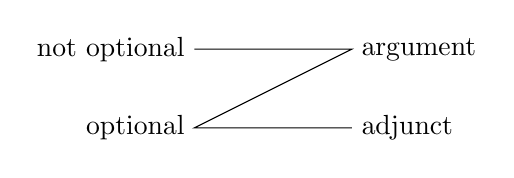
\begin{tikzpicture}
\node[anchor=east](c1) at (-1,2) {not optional};
\node[anchor=east](c2) at (-1,1) {optional};
\node[anchor=west](c3) at (1,2) {argument};
\node[anchor=west](c4) at (1,1) {adjunct};
\draw (c1.east) -- (c3.west) -- (c2.east) -- (c4.west);
\end{tikzpicture}
\caption{\label{fig-optional-arguments-adjuncts}Adjunkte sind immer optional, Argumente können
  optional oder obligatorisch sein \citep[§1182]{Duden2005}}
\end{figure}

Während die Anzahl der Argumente begrenzt ist (durch die Anzahl der verfügbaren Stellen), ist die Anzahl der Adjunkte es nicht: Es kann
beliebig viele Adjunkte in einer Phrase geben. (\mex{1}) zeigt ein Beispiel mit zwei Adjunkten:
\ea
\dass{} der Delphin jetzt dem Kind schnell den Ball gibt
\z

\noindent
Die Analogie mit der Chemie und dem Drama kann verwirrend sein, da H$_2$O ein sehr schönes und stabiles Molekül
ist und es hilfreich ist, sich die parallele Kombination eines Verbs mit seinen beiden
Argumenten vorzustellen. Abbildung~\vref{fig-chemistry-valence} zeigt H$_2$O und die parallele Kombination eines Verbs
mit seinen Argumenten entsprechend (\mex{1}a). Das Problem ist, dass ein einzelnes H und ein O keine
stabile Verbindung bilden, während (\mex{1}b) in Ordnung ist:
\eal
\ex Kirby helps Sandy.
\ex Kirby helps.
\zl
\begin{figure}
\centering
\begin{forest}
[O
  [H] 
  [H] ]
\end{forest}
\hspace{5em}
\begin{forest}
[helps
 [Kirby]
 [Sandy] ]
\end{forest}
\caption{\label{fig-chemistry-valence}Kombination von Wasserstoff und Sauerstoff und die Kombination
eines Verbs mit seinen Argumenten}
\end{figure}%
%\largerpage
Natürlich kann man einfach annehmen, dass es eine Version von \emph{helps} gibt, die eine andere Valenz hat
als die üblicherweise angenommene zweistellige Valenz. Hier bricht die Parallele zusammen, da wir kein
Sauerstoffatom mit nur einer offenen Stelle für das Wasserstoffatom haben. Die Drama-Analogie trägt zur
Verwirrung bei, da das in (\mex{0}b) beschriebene Hilfsereignis natürlich jemanden umfasst, dem geholfen
wird. Die Lösung dieses Problems besteht darin, zwischen syntaktischer und semantischer Valenz zu unterscheiden \citep[Section~3]{Jacobs2003a-u}. Die
Drama-Analogie hilft uns, die semantische Valenz zu finden, die Chemie-Analogie betrifft eher die syntaktische Valenz.

Da Chemie und Drama ihre Probleme haben, können wir auf eine
andere\label{page-shopping-analogy} Analogie zurückgreifen: das Essen. Nehmen wir an, Sie möchten eine Mahlzeit mit Nudeln, Tofu und einer
Tomatensoße zubereiten. Für die Tomatensoße brauchen Sie außerdem ein paar Zwiebeln. Sie setzen alle Zutaten auf eine
Einkaufsliste und gehen in den Laden. Im Laden stellen Sie fest, dass der Tofu ausverkauft ist. Ihre Mahlzeit
funktioniert auch ohne Tofu. Tofu ist optional. Glücklicherweise hat der Laden reichlich Nudeln. Sie können
zwischen den verschiedenen Sorten wählen und die Nudelsorte und Marke auswählen, die Sie bevorzugen. Ein paar Zwiebeln, Tomaten,
und Sie sind fertig. Moment, neben der Kasse liegen diese Gummibärchen. Okay, Sie nehmen auch ein paar davon
mit, obwohl Sie das nicht vorhatten und sie nichts mit Ihrer Mahlzeit und Ihrer Einkaufsliste
zu tun haben. Die Gummibärchen sind die Adjunkte.

Zurück zur Linguistik: Es gibt zwei Wege, sicherzustellen, dass Argumente zusammen mit ihren Köpfen realisiert werden. Der erste
verwendet Techniken, die in Kapitel~\ref{chap-psg-xbar} eingeführt wurden. Wenn man flache Phrasenstrukturregeln
verwendet, kann man sicherstellen, dass bestimmte Argumente zusammen mit bestimmten Köpfen auftreten. Eine
Regel ähnlich der in (\mex{1}) wurde als (\ref{ditrans-schema}) auf Seite~\pageref{ditrans-schema} diskutiert.

\ea
\label{ditrans-schema-two}
\begin{tabular}[t]{@{}l@{ }l@{ }l}
S  & $\to$ & NP[\type{nom}] NP[\type{dat}] NP[\type{acc}] V[\type{ditransitive}]\\
\end{tabular}
\z

\noindent
Solche Schemata wurden in der Generalized Phrase Structure Grammar verwendet \citep*{GKPS85a,Uszkoreit87a}, aber sie wurden
später zugunsten lexikalistischer Modelle aufgegeben, das heißt Modelle, die annehmen, dass Information über die
Argumente eines Kopfes in der lexikalischen Beschreibung des Kopfes statt in Phrasenstrukturregeln
kodiert ist \parencites{Jacobson87b}[Section~5.5]{MuellerGT-Eng1}{MWArgSt}. Gründe für die Aufgabe des phrasalen
Ansatzes der GPSG waren Probleme mit sogenannten Teilvoranstellungen von Verbalphrasen \citep{Nerbonne86a,Johnson86a} und mit der Erfassung von
Interaktionen mit der Morphologie \citep[Section~5.5.1]{MuellerGT-Eng1}.\footnote{%
  Beginnend mit der einflussreichen Arbeit von Adele \citet{Goldberg95a} im Rahmen der Konstruktions"=%
  grammatik\indexcxg{} erlebten die phrasalen Ansätze eine Wiederbelebung \citep{GJ2004a}. Phrasale Ansätze sind weit verbreitet
  und werden auch in anderen Frameworks angenommen
\citep{Haugereid2007a,Haugereid2009a,CJ2005a,Alsina96a,Christie2010a,% resultative constructions as phrasal constructions and
ADT2008a,ADT2013a}.            % argue for a phrasal analysis of the (\ili{Swedish}) caused motion construction.
Die Probleme, die zur Aufgabe der GPSG führten, werden
  in der Literatur ignoriert, und neu eingeführte Probleme werden nicht angemessen behandelt. Siehe
  \cites{Mueller2006d,MuellerPersian,MuellerUnifying,MWArgSt,MWArgStReply,MuellerFCG,MuellerLFGphrasal,MuellerPotentialStructure,MuellerGT-Eng,MuellerCxG}
  für einige Diskussion. Es ist zu beachten, dass es auch lexikalische Varianten der Konstruktions"=%
  grammatik gibt. \citet*{SBK2012a} argumentieren mit der Einführung der \sbcg{} explizit für eine
  lexikalische Sicht und zitieren dabei einige der gerade genannten Quellen. Das Framework, das den in diesem Buch
  skizzierten Vorschlägen zugrunde liegt, ist die Konstruktions-HPSG \citep{Sag97a}.
}

In lexikalischen Ansätzen wird die Valenz eines Kopfes in seinem Lexikoneintrag in Form einer Liste mit Beschreibungen
der Elemente repräsentiert, die zur Valenz des Kopfes gehören. (\mex{1}) gibt einige prototypische Beispiele:
\ea
\label{valence-specifications-German}
\begin{tabular}[t]{@{}l@{~}l@{~}l}
a. & \emph{schläft}:        & \sliste{ NP[\type{nom}] }\\
b. & \emph{kennt}:           & \sliste{ NP[\type{nom}], NP[\type{acc}] }\\
%b. & \emph{unterstützt} `supports':  & \sliste{ NP[\type{nom}], NP[\type{acc}] }\\
c. & \emph{hilft}:           & \sliste{ NP[\type{nom}], NP[\type{dat}] }\\
d. & \emph{gibt}:            & \sliste{ NP[\type{nom}], NP[\type{dat}], NP[\type{acc}] }\\
e. & \emph{wartet}:          & \sliste{ NP[\type{nom}], PP[\type{auf}] }\\
\end{tabular}
\z
Die Elemente in solchen Listen stehen in einer festen Reihenfolge. Die Reihenfolge entspricht der Abfolge der
Elemente im \ili{Englisch}en und der sogenannten unmarkierten Abfolge im \ili{Deutsch}en, das heißt, bei ditransitiven Verben
ist die Abfolge üblicherweise nom, dat, acc (siehe \citew{Hoehle82a} für Anmerkungen zur unmarkierten Abfolge). Diese
feste Abfolge wird verwendet, um die Verknüpfung zwischen Syntax und
Semantik\is{Semantik} herzustellen.\is{linking} Dies wird in Abschnitt~\ref{sec-linking} kurz diskutiert.

Bei einer solchen Valenzrepräsentation für ein Verb wie \emph{kennen} kann man ein Schema annehmen,
das ein Element aus der Valenzliste mit dem jeweiligen Kopf kombiniert und alle ungesättigten
Elemente an das Ergebnis der Kombination weitergibt. Alternativ könnte man eine flache Struktur annehmen, in
der alle Argumente in einem Schritt mit einem Kopf kombiniert werden \parencites[34]{GSag2000a-u}[Section~3]{MuellerOrder}. Ich nehme solche flachen Strukturen nicht an, da
dies die Analyse von Adjunkten (siehe Abschnitt~\ref{sec-adjuncts}) erschweren würde \citep[377--378]{MuellerOrder}.
Der erste Schritt der Analyse von (\mex{1}) ist
in Abbildung~\vref{fig-ihn-kennt} dargestellt.\footnote{%
  Es ist zu beachten, dass dies so klingt, als gäbe es eine Reihenfolge, in der die Dinge kombiniert werden müssen. Dies ist nicht
  der Fall. HPSG-Grammatiken sind Mengen von Beschränkungen, die in beliebiger Reihenfolge angewendet werden können. Es ist nur zu
  Erklärungszwecken, dass Analysen im gesamten Buch von unten nach oben erläutert werden.%
}
\ea
\label{ex-dass-niemand-ihn-kennt}
{}[dass] niemand ihn kennt
\z
\begin{figure}
\centerfit{%
\begin{forest}
sm edges
[{V \sliste{ NP[\type{nom}] } }
  [{NP[\type{acc}]} [ihn] ]
  [{V \sliste{ NP[\type{nom}], NP[\type{acc}] }} [kennt]] ] ]
\end{forest}}
\caption{\label{fig-ihn-kennt}Analyse von \emph{ihn kennt}, die Valenzinformation wird in einer Liste repräsentiert}
\end{figure}
Der Lexikoneintrag für \emph{kennt} hat eine Valenzbeschreibung, die zwei NPs enthält. In einem ersten
Schritt wird \emph{kennt} mit seinem Akkusativobjekt kombiniert. Die resultierende Phrase \emph{ihn kennt}
ist etwas, dessen wichtigste Konstituente ein Verb ist. Daher hat sie V als ihr Kategorie"=%
label. Bestimmte wichtige Eigenschaften linguistischer Objekte werden \emph{Kopfmerkmale}\is{Kopfmerkmal} genannt. Die Wortart
ist eine dieser Eigenschaften. Es wird angenommen, dass alle Kopfmerkmale vom Kopf im Baum
automatisch nach oben weitergegeben werden.

Das Element, das noch nicht mit \emph{kennt} kombiniert wurde, ist die \npnom. Sie ist noch
in der Valenzliste von \emph{ihn kennt} repräsentiert. Abbildung~\vref{fig-niemand-ihn-kennt}
zeigt den nächsten Schritt, bei dem \emph{ihn kennt} mit dem Subjekt \emph{niemand} kombiniert wird.
\begin{figure}
\centerfit{%
\begin{forest}
sm edges
[V \eliste
  [{NP[\type{nom}]} [niemand] ]
  [{V \sliste{ NP[\type{nom}] } }
    [{NP[\type{acc}]} [ihn] ]
    [{V \sliste{ NP[\type{nom}], NP[\type{acc}] }} [kennt]] ] ]
\end{forest}}
\caption{\label{fig-niemand-ihn-kennt}Analyse von (\emph{dass}) \emph{niemand ihn kennt}}
\end{figure}
Das Ergebnis ist ein linguistisches Objekt der Kategorie Verb mit der leeren Liste als Valenzrepräsentation.

Wie in Kürze gezeigt wird, ist das Schema, das Strukturen wie das V \eliste{} und V \sliste{ NP[\type{nom}] } in
Abbildung~\ref{fig-niemand-ihn-kennt} lizenziert, eine abstraktere Version der Regel in (\ref{psg-binaer}) auf Seite~\pageref{psg-binaer}.

% This can be depicted as in
% Figure~\vref{fig-valence-German}, which is an example analysis of (\mex{1}).
% \ea
% \label{ex-dass-niemand-ihn-kennt}
% \gll  {}[dass] niemand ihn kennt\\
%       \spacebr{}that nobody.\NOM{} him.\ACC{} knows\\ 
% \glt `that nobody knows him'
% \z
% \begin{figure}
% \centerfit{%
% \begin{forest}
% sm edges
% [{S \eliste}
%   [{NP[\type{nom}]} [niemand;nobody] ]
%   [{V$'$\sliste{ NP[\type{nom}] } }
%     [{NP[\type{acc}]} [ihn;him] ]
%     [{V \sliste{ NP[\type{nom}], NP[\type{acc}]}} [kennt;knows]] ] ]
% \end{forest}}
% \caption{\label{fig-valence-German}Analysis of (\emph{dass}) \emph{niemand ihn kennt} `that nobody
%   knows him', valence information is represented in a list}
% \end{figure}

% The lexical item for \emph{kennt} `knows' has a valence description containing two NPs. In a first
% step \emph{kennt} is combined with its accusative object. The resulting phrase \emph{ihn kennt} `him
% knows' is something whose most importent constituent is a verb. Therefore it has a V in its category
% label. Since \emph{ihn kennt} is not a sentence but something intermediate, it gets the label
% V$'$.\footnote{%
%   These labels are abbreviations for complex categories. Their internal makeup is given in
%   Table~\ref{tab-abbreviations-v-vbar-s} on p.\,\pageref{tab-abbreviations-v-vbar-s}. The labels are
%   similar to what is known from \xbart, but -- as was already mentioned in the previous chapter --
%   the theory developed here is not following all the tenets of \xbart. For example, simple nouns
%   like \emph{house} are N$'$ and there is no \nnull in the analysis of NPs like \emph{the house}.

%   Section~\ref{sec-intro-spr-comps} explains why the abbreviation for \emph{ihn kennt} `him knows' is V$'$ rather than VP.
% }
%
% The nodes for V$'$ and S are licensed by a schema that combined a head with one element of its
% valence list. The full schema will be given in Chapter~\ref{chap-HPSG-light}, but we will discuss a
% simplified version of it in Section~\ref{sec-intro-schemata}.

Es ist wahrscheinlich hilfreich, zu unserer Analogie vom Einkaufen für eine Mahlzeit zurückzukehren. Nehmen wir an, wir verwenden eine App, um
unsere Einkaufslisten zu organisieren. Für unsere aktuelle Mahlzeit brauchen wir Nudeln und Tomaten. Sie sind in der
App in einer bestimmten Reihenfolge aufgeführt (Tomaten, Nudeln), und es sind kleine Bilder an den Produkten angebracht. Sobald
wir etwas gefunden haben, das zu den Nudeln passt, entfernen wir die Nudeln von der Liste, und die verbleibende Liste
enthält ein Symbol, das uns an die Tomaten erinnert. Sobald wir diese haben, entfernen wir sie von der Liste, und
da nichts mehr auf der Liste steht, bezahlen wir. Linguistische Strukturen sind ähnlich: Wir beginnen
mit einem Verb, das zwei NPs selegiert, kombinieren es mit einer NP und dann mit der zweiten. Das Ergebnis ist
eine vollständige Struktur, etwas mit einer leeren Valenzliste.

Es gibt verschiedene Wege, mit optionalen Argumenten umzugehen. Der einfachste ist, weitere
Lexikoneinträge anzunehmen, die weniger Argumente selegieren. Für das Beispiel in (\ref{ex-sie-gibt}) würde man die Valenz"=%
repräsentation in (\mex{1}a) annehmen, und für Sätze mit \emph{warten} ohne Präpositional"=%
objekt würde man (\mex{1}b) zusätzlich zu den Repräsentationen in (\ref{valence-specifications-German}) annehmen:
\ea
\begin{tabular}[t]{@{}l@{~}l@{~}l}
a. & \emph{gibt}:            & \sliste{ NP[\type{nom}] }\\
b. & \emph{wartet}:          & \sliste{ NP[\type{nom}] }\\
\end{tabular}
\z
\is{Valenz|)}

\section{Scrambling: Die allgemeine Idee}
\label{sec-scrambling}

Wie\is{Scrambling|(}\is{Abfolge|(} wir bereits in der Datendiskussion in Abschnitt~\ref{sec-phenomenon-scrambling} gesehen haben, erlauben manche Sprachen
das Scrambling von Argumenten. Für diese Sprachen kann man annehmen, dass ein Kopf mit jedem seiner
Argumente kombiniert werden kann, nicht notwendigerweise beginnend mit dem letzten, wie es bei der Analyse in Abbildung~\ref{fig-niemand-ihn-kennt} der Fall war.
Abbildung~\vref{fig-scrambling-German} zeigt die Analyse von (\mex{1}).
\ea
{}[dass] ihn niemand kennt
\z
\begin{figure}
\centerfit{%
\begin{forest}
sm edges
[{V \eliste}
   [{NP[\type{acc}]} [ihn] ]
   [{V \sliste{ NP[\type{acc}] } }
      [{NP[\type{nom}]} [niemand] ]
      [{V \sliste{ NP[\type{nom}], NP[\type{acc}] }} [kennt] ] ] ]
\end{forest}}
\caption{\label{fig-scrambling-German}Analyse von (\emph{dass}) \emph{ihn niemand kennt};
  Sprachen, die Scrambling erlauben, gestatten die Sättigung von Argumenten in beliebiger Reihenfolge}
\end{figure}
Statt das Verb zuerst mit dem Akkusativargument (dem Objekt) zu kombinieren, wird es mit dem
Nominativ (dem Subjekt) kombiniert, und der Akkusativ (das Objekt) wird in einem späteren Schritt hinzugefügt.%
\is{Scrambling|(}\is{Abfolge|(}

% only for unstressed pronouns.
%Such an analysis predicts that reorderings of arguments are possible in principle and this is
%independent of the question whether arguments are pronominal or not. However, some authors claim
%that the order of pronouns is rigid \citep[131]{Haider2010a}.

\section{SVO: Sprachen mit fester SV-Abfolge und Valenzmerkmalen}
\label{sec-intro-schemata}
\label{sec-intro-spr-comps}

Der letzte Abschnitt hat gezeigt, wie verbletzte Sätze im \ili{Deutsch}en analysiert werden können. Natürlich ist es
leicht vorstellbar, wie sich dies auf VSO-Sprachen erweitert: Der Kopf ist initial und kombiniert sich zuerst mit dem ersten
Element in der Valenzliste und dann mit allen anderen Elementen. Über SVO-Sprachen wurde bislang jedoch nichts
gesagt. In Sprachen wie dem \ili{Dänisch}en, dem \ili{Englisch}en und so weiter werden alle Objekte
nach dem Verb realisiert, wie in (\mex{1}); nur das Subjekt steht vor dem Verb.
\ea
Kim gave Sandy the book.
\z
Das Verb bildet zusammen mit seinen Objekten in einem bestimmten Sinne eine Einheit: Es kann vorangestellt werden (\mex{1}a). Es kann von
dominierenden Verben selegiert werden (\mex{1}b), es kann koordiniert werden\is{Koordination} (\mex{1}c), und es ist der Ort, an den sich Adjunkte anlagern (\mex{1}d--e).
\eal
\ex John promised to read the book and [read the book], he will.
\ex He will [read the book].
\ex Kim [[sold the car] and [bought a bicycle]].
\ex He often [reads the book].
%\ex He [reads the book] often.
\ex \ldots{} [often [read the book] slowly], he will.
\zl
Dies kann angemessen modelliert werden, indem man zwei Valenzlisten annimmt: eine für die Komplemente\is{Komplement} (\comps{} kurz für \textsc{complements}\isfeat{comps}) und
eine für das Subjekt\is{Subjekt}. Die Liste für das Subjekt wird \textsc{specifier}\is{Spezifikator}-Liste
(\spr) genannt.\isfeat{spr}\footnote{%
  Es gibt verschiedene Versionen der HPSG: \citet[Chapter~3.2]{ps} nahm an, dass alle Argumente eines Kopfes
  in einer Liste repräsentiert werden. Diese Liste wurde \subcatl{} genannt. \citet{Borsley87a} argumentierte, dass man
  mehrere Valenzmerkmale (\subj, \spr und \comps) verwenden sollte, und dies wurde in
  \citew[Chapter~9]{ps2} übernommen: Subjekte von Verben wurden über \subj{} selegiert und Determinatoren über
  \spr. \citet*[Chapter~4.3]{SWB2003a} nehmen an, dass sowohl Subjekte als auch Determinatoren über \spr{} selegiert werden, was
  auch in den hier entwickelten Grammatiken angenommen wird. \citet[Section~3.3]{Sag2012a} präsentiert eine Version der HPSG
  namens Sign-Based Construction Grammar (SBCG), die wie 1987 üblich eine Valenzliste für alle Argumente
  annimmt. Diese Rückkehr zu einem aufgegebenen Ansatz kam ohne jede Argumentation. Daher übernehme ich diese
  Variante der HPSG nicht, sondern halte an der Trennung von Subjekten und anderen Argumenten auf \spr{} und \comps{} fest. Ich
  werde \subj{} nicht als Valenzmerkmal verwenden, aber es wird in der Analyse der Verbalkomplexe
  in Kapitel~\ref{chap-verbal-complex} eingeführt.
} Die Spezifikatorliste spielt sowohl in der Analyse von Sätzen als auch in der Analyse von Nominalphrasen eine Rolle. Nomina
selegieren ihren Determinator über \spr{} und alle ihre anderen Argumente über \comps. Abbildung~\vref{fig-svo}
zeigt die Analyse von Satz (\mex{1}) unter Verwendung der Merkmale \spr{} und \comps.
\ea
Nobody knows him.
\z
\begin{figure}
\centerfit{%
\begin{forest}
sm edges
[{V[\spr \eliste, \comps \eliste]}, name=S
   [{NP[\type{nom}]} [nobody] ]
   [V\feattab{
      \spr \sliste{ NP[\type{nom}] }, \comps \sliste{}}, name=VP
     [V\feattab{
         \spr \sliste{ NP[\type{nom}] },\\
         \comps \sliste{ NP[\type{acc}] }} [knows] ]
        [{NP[\type{acc}]} [him] ] ] ]
\node [right=4cm] at (S)
    {
        = S
    };
\node [right=4cm] at (VP)
    {
        = VP
    };
\end{forest}}
\caption{\label{fig-svo}Analyse der SVO-Abfolge mit zwei getrennten Valenzmerkmalen}
\end{figure}
Die \compsl{} von \emph{knows} enthält eine Beschreibung des Akkusativobjekts, und der Akkusativ
\emph{him} wird in einem ersten Schritt mit \emph{knows} kombiniert. Zusätzlich zum Akkusativobjekt
selegiert \emph{knows} ein Subjekt. Diese Selektion wird an den Mutterknoten, die VP, weitergegeben. Daher ist
der \sprv{} von \emph{knows him} identisch mit dem \sprv{} von \emph{knows}. Die VP \emph{knows him}
selegiert eine Nominativ-NP. Diese NP ist in Abbildung~\ref{fig-svo} als \emph{nobody} realisiert. Das
Ergebnis der Kombination von \emph{knows him} mit \emph{nobody} ist \emph{nobody knows him}, was
vollständig ist: Es hat sowohl eine leere \sprl{} als auch eine leere \compsl. Die beiden Regeln, die für
die Kombinationen in Abbildung~\ref{fig-svo} verantwortlich sind, heißen Spezifikator-Kopf-Schema und
Kopf-Komplement-Schema. Ich verwende VP als Abkürzung für etwas mit verbalem Kopf und einer leeren \compsl{} und mindestens
einem Element in der \sprl, und S als Abkürzung für etwas mit verbalem Kopf und leeren Listen sowohl
für \spr{} als auch \compsv.

In Abschnitt~\ref{sec-scrambling} wurde erklärt, wie Scrambling erfasst werden kann: Die Regeln, die
Köpfe mit ihren Argumenten kombinieren, können die Argumente in beliebiger Reihenfolge von der Liste nehmen. Für Sprachen
mit strengeren Anforderungen an die Konstituentenabfolge sind die Regeln strenger: Die Argumente müssen
konsequent vom Anfang oder vom Ende der Liste genommen werden. So beginnt man für das \ili{Englisch}e und das \ili{Dänisch}e
am Anfang der Liste, und für kopffinale Sprachen ohne Scrambling beginnt man am Ende
der Liste. Abbildung~\ref{fig-svo-ditrans} zeigt die Analyse eines Satzes mit einem ditransitiven Verb.
\begin{figure}
\centerfit{%
\begin{forest}
sm edges
[{V[\spr \eliste, \comps \eliste]}
   [{NP[\type{nom}]} [Kim] ]
   [V\feattab{
      \spr \sliste{ NP[\type{nom}] }, \comps \sliste{}}
     [V\feattab{
         \spr \sliste{ NP[\type{nom}] },\\
         \comps \sliste{ PP[\type{to}] }}
       [V\feattab{
           \spr \sliste{ NP[\type{nom}] },\\
           \comps \sliste{ NP[\type{acc}], PP[\type{to}] }} [gave] ]
         [{NP[\type{acc}]} [a book, roof] ] ]
       [{PP[\type{to}]} [to Sandy, roof] ] ] ]
\end{forest}}
\caption{\label{fig-svo-ditrans}Analyse der SVO-Abfolge mit zwei getrennten Valenzmerkmalen und zwei
  Elementen in \comps}
\end{figure}
Das Akkusativobjekt ist das erste Element in der \compsl{} und wird zuerst mit dem Verb
kombiniert. Das Ergebnis der Kombination ist eine verbale Projektion, die die PP[\type{to}] als einziges
Element in der \compsl{} hat. Sie wird im nächsten Schritt mit einer passenden PP kombiniert, was zu einer verbalen
Projektion mit einer leeren \compsl{} (einer VP) führt.

Die Analyse unseres ersten \ili{Deutsch}en Beispiels in Abbildung~\ref{fig-niemand-ihn-kennt} verwendete keinen Namen
für die Valenzliste. Die Frage ist also: Wie verhält sich die Analyse des \ili{Deutsch}en zur Analyse des
\ili{Englisch}en mit \spr{} und \comps? Viele Forscher aus verschiedenen Frameworks haben argumentiert, dass es nicht
sinnvoll ist, in Grammatiken des \ili{Deutsch}en die Subjekte finiter Verben von anderen Argumenten zu unterscheiden. Alle Tests, die
verwendet wurden, um zu zeigen, dass sich Subjekte im \ili{Englisch}en von Komplementen unterscheiden, gelten nicht für die Argumente
finiter Verben im \ili{Deutsch}en. Zum Beispiel wird argumentiert, dass Subjekte -- im Gegensatz zu Objekten --
Extraktionsinseln sind\is{Insel} \parencites[\page 249--250]{Chomsky73a}[\page 76]{Fanselow87a}[\page 35--36]{Grewendorf89a}, das heißt, nichts kann
aus einem Subjekt vorangestellt werden. Aber \citet[\page 173]{Haider93a} zeigt anhand der Beispiele in (\mex{1}), dass dies für das
\ili{Deutsch}e nicht gilt.
% Haider2010: 23 allgemein für OV/VO
% Haider 2010: 40 zitiert Haider83 und Haider89
\eal
\ex {}[Über Strauß]$_i$ hat [ein Witz \_$_i$] die Runde gemacht.
\ex {}[Zu drastischeren Maßnahmen]$_i$ hat ihm [der Mut \_$_i$] gefehlt.
\ex {}[Zu diesem Problem]$_i$ haben uns noch [einige Briefe \_$_i$] erreicht.\footnote{\citew[\page 79]{Oppenrieder91a}
}

\zl

%\enlargethispage{3pt}
\noindent
Das \_$_i$ zeigt die Stelle an, an die das vorangestellte Element, das Element im \vf, gehört. Es befindet sich in
allen drei Beispielen innerhalb der Subjekt-NP. Da es im \ili{Deutsch}en keine Subjekt-Objekt-Asymmetrien gibt,
haben Forscher wie \citet[\page 295]{Pollard90a}, \citet[Section~6.3.2]{Haider93a}, \citet[\page
376]{Eisenberg94b} und \citet[\page 57, 78]{Kiss95a} für sogenannte „Subjekt-als-Komplement``-Analysen argumentiert.
Abbildung~\vref{fig-spr-german} zeigt die angepasste Analyse von
(\ref{ex-dass-niemand-ihn-kennt}) -- hier wiederholt als
(\ref{ex-dass-niemand-ihn-kennt-two}):
\ea
\label{ex-dass-niemand-ihn-kennt-two}
{}[dass] niemand ihn kennt
\z
\begin{figure}
\centerfit{%
\begin{forest}
sm edges
[{V[\spr \eliste, \comps \eliste]}, name=S
        [{NP[\type{nom}]} [niemand] ]
        [{V\feattab{
              \spr \eliste, \comps \sliste{ NP[\type{nom}] } }}, name = Vs
          [{NP[\type{acc}]} [ihn] ]
          [V\feattab{
              \spr \eliste,\\
              \comps \sliste{ NP[\type{nom}], NP[\type{acc}]}} [kennt] ]
] ]
\node [right=4cm] at (S)
    {
        = S
    };
\node [right=4cm] at (Vs)
    {
        = V$'$
    };
\end{forest}}
\caption{\label{fig-spr-german}Die Analyse eines deutschen Satzes mit \spr{} und \compsl}
\end{figure}
%\largerpage
Der Unterschied zwischen dem \ili{Deutsch}en und dem \ili{Englisch}en besteht darin, dass das \ili{Deutsch}e alle Argumente in der \compsl{} des
finiten Verbs enthält und keine Argumente in der \sprl. Da die Elemente in der \compsl{} in beliebiger Reihenfolge mit
dem Kopf kombiniert werden können, ist erklärt, warum alle Permutationen von Argumenten
möglich sind. Spezifikatoren werden links von ihrem Kopf realisiert. Dies ist im \ili{Deutsch}en und
\ili{Englisch}en gleich. Für das \ili{Deutsch}e ist dies im verbalen Bereich nicht relevant, aber das Spezifikator-Kopf-Schema, das
in Kürze eingeführt wird, wird in der Analyse von Nominalphrasen verwendet.

Im weiteren Verlauf dieses Buches verwende ich die Abkürzungen in Tabelle~\vref{tab-abbreviations-v-vbar-s}.
\begin{table}
 \begin{tabular}[t]{@{}l@{ = }l}\lsptoprule
             S  & V[\spr \eliste, \comps \eliste]\\
             VP & V[\spr \sliste{ NP[\type{nom}] }, \comps \sliste{}]\\
             V$'$ & alle anderen V-Projektionen außer Verbalkomplexen\\[2pt]
             NP & N[\spr \eliste, \comps \eliste]\\
             N$'$ & N[\spr \sliste{ Det }, \comps \sliste{}]\\\lspbottomrule
             \end{tabular}
\caption{\label{tab-abbreviations-v-vbar-s}Abkürzungen für S, VP und V$'$ sowie NP, N$'$}
\end{table}

\section{Schemata der unmittelbaren Dominanz}

In Abschnitt~\ref{sec-valence} habe ich bereits erwähnt, dass die Nichtterminalknoten in einem Baum, das heißt die
Knoten, die nicht die Blätter des Baumes sind, durch Schemata lizenziert werden, die denen ähneln, die in
Kapitel~\ref{sec-PSG-Merkmale} und~\ref{sec-xbar} eingeführt wurden. Tatsächlich sind die Schemata sogar abstrakter als
\xbar-Schemata, da sie keine Aussagen über die lineare Abfolge der Töchter machen. Die
beiden in diesem Abschnitt diskutierten Schemata sind hier als (\mex{1}) skizziert:
\ea\label{schema-head-spr-and-head-comps-preliminary}
Spezifikator-Kopf\is{schema!Specifier-Head}-Schema und Kopf-Komplement\is{schema!Head-Complement}-Schema (vorläufig)
\begin{tabular}[t]{@{}l@{ }l@{}}
H[\spr \ibox{1}]   & $\to$ H[\spr \ibox{1} $\oplus$ \sliste{ \ibox{2} }, \comps \eliste]\hspace{1em}\ibox{2}  \\
H[\comps \ibox{1}] & $\to$ H[\comps \sliste{ \ibox{2} } $\oplus$ \ibox{1}]\hspace{1em}\ibox{2} \\
\end{tabular}
\z

\noindent
Syntaktische Regeln, wie sie hier verwendet werden, werden üblicherweise Schemata genannt, da sie recht abstrakt sind: Sie
nennen keine spezifischen Kategorien, sondern identifizieren stattdessen bestimmte Information in den Mutter- und Tochterbeschreibungen.
%The details about such schemata will be given in Chapter~\ref{chap-HPSG-light},
Die Details zu solchen Schemata werden in formalerer HPSG-Literatur wie
\citew[Chapter~4]{MuellerLehrbuch3} oder \citew{Abeille:Borsley2021a} angegeben,
aber Abbildung~\vref{fig-spr-head} und
Abbildung~\vref{fig-head-comp} liefern die jeweiligen Baumdarstellungen.
\begin{figure}
\begin{forest}
[H\feattab{\spr \ibox{1}}%,\\
           %\comps \eliste}
  [\ibox{2}]
  [H\feattab{\spr \ibox{1} $\oplus$ \sliste{ \ibox{2} },\\
             \comps \eliste}
  ]]
\end{forest}
\caption{\label{fig-spr-head}Skizze des Spezifikator-Kopf\is{schema!Specifier-Head}-Schemas (vorläufig)}
\end{figure}
Das H steht für \emph{head} (Kopf). Der Begriff \term{Kopftochter} wird für die Tochter verwendet, die entweder
der Kopf einer Phrase ist oder den Kopf der Phrase enthält (\zb das Verb in einem Satz oder das Nomen in einer
Nominalphrase). \emph{append} ($\oplus$) ist eine Relation, die zwei
Listen verkettet. Zum Beispiel ist die Verkettung von \sliste{ \normalfont a } und \sliste{ \normalfont b }
\sliste{ \normalfont a, b }. Die Verkettung der leeren Liste \eliste{} mit einer anderen Liste ergibt
die letztere Liste. Um einige Beispiele zu geben, die in diesem Kapitel relevant sind, betrachte man die Liste
\sliste{ NP[\type{nom}], NP[\type{dat}], NP[\type{acc} ] }. \emph{append} kann verwendet werden, um zwei
Listen aneinanderzuhängen, was unsere Liste auf die folgenden Weisen ergibt:
\eal
\ex \eliste{} $\oplus$ \sliste{ NP[\type{nom}], NP[\type{dat}], NP[\type{acc}] } = \sliste{ NP[\type{nom}], NP[\type{dat}], NP[\type{acc}] }
\ex \sliste{ NP[\type{nom}] } $\oplus$ \sliste{ NP[\type{dat}], NP[\type{acc}] } = \sliste{ NP[\type{nom}], NP[\type{dat}], NP[\type{acc}] }
\ex \sliste{ NP[\type{nom}], NP[\type{dat}] } $\oplus$ \sliste{ NP[\type{acc}] } = \sliste{ NP[\type{nom}], NP[\type{dat}], NP[\type{acc}] }
\ex \sliste{ NP[\type{nom}], NP[\type{dat}], NP[\type{acc}] } $\oplus$ \eliste{} = \sliste{ NP[\type{nom}], NP[\type{dat}], NP[\type{acc}] }
\zl
Das Schema in Abbildung~\ref{fig-spr-head} zerlegt eine Liste so, dass eine Liste mit einem
einzelnen Element ( \sliste{ \ibox{2} } ) und eine Restliste \iboxb{1} entstehen. Nimmt man die
dreielementige Liste mit nom-, dat- und acc-Elementen an, so wäre dies in (\mex{0}c) der Fall, und \ibox{2} wäre NP[\type{acc}] und
\ibox{1} wäre \sliste{ NP[\type{nom}], NP[\type{dat}] }. In diesem Buch hat die \sprl{} höchstens ein Element.\footnote{
  Siehe aber \citew{MOe2013b} für eine Analyse des \isi{object shift}s im \ili{Dänisch}en, die mehrere Elemente in
  der \sprl{} annimmt.
} Es kann eine NP[\type{nom}] im Falle von Verben in den SVO-Sprachen sein oder der Determinator, wenn
der Kopf ein Nomen ist. Wenn man eine Liste mit einem einzelnen Element in eine Liste mit einem Element
und einen Rest aufspaltet, ist der Rest immer die leere Liste. Daher ist \ibox{1} bei den Listen auf der rechten Seite der Gleichungen in (\mex{1}) die
leere Liste, und \ibox{2} ist NP[\type{nom}] bzw.\ Det.
\eal
\ex \eliste{} $\oplus$ \sliste{ NP[\type{nom}] } = \sliste{ NP[\type{nom}] }
\ex \eliste{} $\oplus$ \sliste{ Det } = \sliste{ Det }
\zl

\noindent
Damit ein Schema wie das in Abbildung~\ref{fig-spr-head} anwendbar ist, müssen die Beschreibungen der
Töchter mit den tatsächlichen Töchtern übereinstimmen. Zum Beispiel ist \emph{sleeps} mit der
rechten Tochter kompatibel: Es hat eine NP[\type{nom}] in seiner \sprl. Wenn \emph{sleeps} als
Tochter des Schemas in Abbildung~\ref{fig-spr-head} realisiert wird, wird \ibox{2} als
NP[\type{nom}] instantiiert. Daher muss die linke Tochter mit einer NP[\type{nom}] kompatibel sein. Sie kann
als einfaches Pronomen wie \emph{she} oder als komplexe NP wie \emph{the brown squirrel} realisiert werden. Zwei
Analysen sind in Abbildung~\ref{fig-she-sleeps-the-brown-squirrel-sleeps} dargestellt.
\begin{figure}
\hfill
\begin{forest}
sm edges
[V\feattab{\spr \eliste,\\
           \comps \eliste}
  [{\ibox{1} NP[\type{nom}]} [she]]
  [V\feattab{\spr \sliste{ \ibox{1} NP[\type{nom}] },\\
             \comps \eliste} [sleeps]]]
\end{forest}
\hfill
\begin{forest}
sm edges
[V\feattab{\spr \eliste,\\
           \comps \eliste}
  [{\ibox{1} NP[\type{nom}]} [the brown squirrel,roof]]
  [V\feattab{\spr \sliste{ \ibox{1} NP[\type{nom}] },\\
             \comps \eliste} [sleeps]]]
\end{forest}\hfill\mbox{}
\caption{Kopf-Spezifikator-Phrasen mit einem Subjekt und einem intransitiven Verb}\label{fig-she-sleeps-the-brown-squirrel-sleeps}
\end{figure}
Das \ibox{1} in Abbildung~\ref{fig-she-sleeps-the-brown-squirrel-sleeps} besagt, dass das, was in der
\sprl{} steht, mit dem identifiziert wird, was das andere Element im Baum ist. Ich habe \npnom{} sowohl im NP-Knoten als auch innerhalb der \sprl{} hinter
das \ibox{1} geschrieben, aber es hätte gereicht, \npnom{}
an einer der beiden Stellen zu erwähnen. Die tatsächliche Zahl in der Box spielt keine Rolle. Worauf es ankommt, ist, wo dieselbe
Zahl in den Bäumen oder Strukturen erscheint. Ich beginne üblicherweise mit \ibox{1} an der Spitze des Baumes und
verwende fortlaufende Zahlen für die folgenden Identifikationen.

Abbildung~\ref{fig-nobody-gave-the-child-a-book} auf S.\,\pageref{fig-nobody-gave-the-child-a-book}
unten zeigt eine Beispielanalyse mit einem ditransitiven Verb, an der ebenfalls das Spezifikator-Kopf-Schema
beteiligt ist. Die Spezifikation des \compsv{} der Kopftochter im Spezifikator-Kopf-Schema stellt sicher,
dass das Verb mit seinen Komplementen kombiniert wird, bevor der Spezifikator hinzugefügt wird.

Neben seiner Verwendung für die Analyse von Subjekt"=VP-Kombinationen in den SVO-Sprachen wird das Spezifikator-Kopf-Schema auch
für die Analyse von NPs in allen \ili{germanisch}en Sprachen verwendet. Abbildung~\ref{fig-spr-head-the-squirrel} zeigt die Analyse der NP \emph{the squirrel}.
\begin{figure}
\begin{forest}
[{N[\spr \eliste, \comps \eliste]}
  [\ibox{1} Det [the]]
  [{N[\spr \sliste{ \ibox{1} }, \comps \eliste]} [squirrel]]]
\end{forest}
\caption{\label{fig-spr-head-the-squirrel}Analyse der NP \emph{the squirrel}}
\end{figure}
\emph{squirrel} selegiert einen Determinator, und das Ergebnis der Kombination von \emph{squirrel} mit einem Determinator ist eine
vollständige nominale Projektion, das heißt eine NP. Es gibt auch Nomina wie \emph{picture}, die zusätzlich zu einem
Determinator ein Komplement nehmen:
\ea
a picture of Kim
\z
Die Kombination von \emph{picture} und seinem Komplement \emph{of Kim} ist parallel zur Kombination
eines Verbs mit seinem Objekt in VO-Sprachen mit fester Konstituentenabfolge. Für solche Kombinationen brauchen wir ein eigenes Schema: das Kopf-Komplement-Schema,
das in Abbildung~\ref{fig-head-comp} angegeben ist.
\begin{figure}
\begin{forest}
[{H[\comps \ibox{1}]}
  [{H[\comps  \sliste{ \ibox{2} } $\oplus$ \ibox{1}  ]}]
  [\ibox{2}]]
\end{forest}
\caption{\label{fig-head-comp}Skizze des Kopf-Komplement\is{schema!Head-Complement}-Schemas (vorläufig)}
\end{figure}
%\largerpage
Das Schema spaltet die \compsl{} eines Kopfes in eine Anfangsliste mit einem Element \iboxb{2} auf, das
als Komplementtochter rechts realisiert wird.\footnote{%
  Im Prinzip sind Töchter in der HPSG ungeordnet, so wie sie es in der GPSG waren \citep{GKPS85a}. Spezielle Linearisierungsregeln werden
  verwendet, um einen Kopf relativ zu seinen Geschwistern in einem lokalen Baum zu ordnen. Ein Schema, das einen Baum
  wie den in Abbildung~\ref{fig-head-comp} lizenziert, würde also auch einen Baum mit den Töchtern in einer
  anderen Reihenfolge lizenzieren, sofern man keine Linearisierungsregeln hätte, die dies ausschließen. Siehe
  \citew{MuellerOrder} für einen Überblick über Ansätze zur Konstituentenabfolge in der HPSG. Lineare Präzedenz"=%
  regeln werden in Abschnitt~\ref{sec-lp-rules} ausführlicher diskutiert.
}
Dieses Schema lizenziert sowohl die Kombination von \emph{gave} und \emph{the child} als auch die Kombination von
\emph{gave the child} und \emph{a book} in Abbildung~\vref{fig-nobody-gave-the-child-a-book}, die die
Analyse von (\mex{1}) zeigt.\footnote{%
  \ili{Englisch}e Nomina und Determinatoren flektieren nicht nach Kasus. Der Kasus zeigt sich jedoch in Pronomina:
  \emph{he} (Nominativ), \emph{his} (Genitiv), \emph{him} (Akkusativ). Daher selegieren Verben in Doppelobjekt"=%
  konstruktionen zwei Akkusative statt eines Dativs und eines Akkusativs wie im \ili{Deutsch}en.
}
\ea
\label{ex-nobody-gave-the-child-a-book}
Nobody gave the child a book.
\z
\begin{figure}
\centerfit{%
\begin{forest}
sm edges
[{V[\spr \eliste, \comps \eliste]}
   [{\ibox{1} NP[\type{nom}]} [nobody] ]
   [V\feattab{
      \spr \sliste{ \ibox{1} NP[\type{nom}] }, \comps \sliste{}}
     [V\feattab{
         \spr \sliste{ \ibox{1} NP[\type{nom}] },\\
         \comps \sliste{ \ibox{2} NP[\type{acc}] }} 
        [V\feattab{
           \spr \sliste{ \ibox{1} NP[\type{nom}] },\\
           \comps \sliste{ \ibox{3} NP[\type{acc}], \ibox{2} NP[\type{acc}]}} [gave] ]
        [{\ibox{3} NP[\type{acc}]} [the child,roof] ] ]
     [{\ibox{2} NP[\type{acc}]} [a book,roof ] ] ] ]
\end{forest}}
\caption{\label{fig-nobody-gave-the-child-a-book}Analyse der Sätze mit einem ditransitiven Verb}
\end{figure}

Um die Dinge einfach zu halten, erwähnte das Spezifikator-Kopf\is{schema!Specifier-Head}-Schema den \compsv{} der Mutter nicht. Das
Kopf-Komplement-Schema erwähnte weder den \sprv{} der Kopftochter noch den der Mutter. Aber die
jeweiligen Werte sind wichtig, da über diese Werte in Strukturen, die durch diese Schemata lizenziert werden,
etwas gesagt werden muss. Wenn der \sprv{} in der Kombination von \emph{gave} und \emph{the
  child} durch das Kopf-Komplement-Schema nicht eingeschränkt würde, wäre jeder Wert möglich. Dies
schließt eine \sprl{} ein, die zwei Genitiv-NPs und eine Akkusativ-NP enthält. Folgen wie (\mex{1}) wären
lizenziert:

\ea[*]{
his his him gave the child a book
}
\z
Um solche unspezifizierten \sprv{}e zu vermeiden, wird der \sprv{} der Kopftochter im Schema mit dem \sprv{} des
Mutterknotens identifiziert. Dies ist das \ibox{1} in (\mex{1}b). Ebenso muss der \compsv{} der Mutter
in Spezifikator-Kopf-Phrasen als identisch mit dem \compsv{} der Kopftochter spezifiziert werden
(\ibox{2} in (\mex{1}a)) und somit als die leere Liste.

\ea\label{schema-head-spr-and-head-comps}
Spezifikator-Kopf\is{schema!Specifier-Head}-Schema und Kopf-Komplement\is{schema!Head-Complement}-Schema (endgültig)
\begin{tabular}[t]{@{}l@{~}l@{ }l@{}}
a. & H[\spr \ibox{1}, \comps \ibox{2}] & $\to$ H[\spr \ibox{1} $\oplus$ \sliste{ \ibox{3} }, \comps \ibox{2} \eliste]\hspace{1em}\ibox{3}  \\
b. & H[\spr \ibox{1}, \comps \ibox{2}] & $\to$ H[\spr \ibox{1}, \comps \ibox{2} $\oplus$ \sliste{ \ibox{3} }]\hspace{1em}\ibox{3} \\
\end{tabular}
\z
Abbildung~\vref{fig-spr-head-head-comps-final} zeigt die endgültigen Versionen der beiden Schemata.
\begin{figure}
\hfill
\begin{forest}
[H\feattab{\spr \ibox{1},\\
           \comps \ibox{2}}
  [\ibox{3}]
  [H\feattab{\spr \ibox{1} $\oplus$ \sliste{ \ibox{3} },\\
              \comps \ibox{2} \eliste}]]
\end{forest}
\hfill
\begin{forest}
[H\feattab{\spr \ibox{1},\\
           \comps \ibox{2}}
  [H\feattab{\spr \ibox{1},\\
             \comps  \sliste{ \ibox{3} } $\oplus$ \ibox{2}  ]}]
  [\ibox{3}]]
\end{forest}
\hfill\mbox{}
\caption{\label{fig-spr-head-head-comps-final}Skizze des Spezifikator-Kopf\is{schema!Specifier-Head}- und Kopf-Komplement\is{schema!Head-Complement}-Schemas}
\end{figure}

\section{Scrambling: Die Details}

Um\is{Scrambling|(}\is{Abfolge|(} nun Sprachen mit freier Konstituentenabfolge zu analysieren, wird eine liberalere Variante
des Schemas in Abbildung~\ref{fig-head-comp} benötigt. Abbildung~\vref{fig-head-comp-free} spaltet die \compsl{} eines
Kopfes in drei Teile auf: eine Liste \ibox{1}, eine Liste mit genau einem Element \sliste{ \ibox{3} }
und eine dritte Liste \ibox{2}. Das Element der zweiten Liste wird als das Komplement des Kopfes realisiert.
\begin{figure}
\begin{forest}
[{H[\comps \ibox{1} $\oplus$ \ibox{2}]}
  [\ibox{3}]
  [{H[\comps  \ibox{1} $\oplus$ \sliste{ \ibox{3} } $\oplus$ \ibox{2}  ]}]]
\end{forest}
\caption{\label{fig-head-comp-free}Skizze des Kopf-Komplement-Schemas für Sprachen mit freier
  Konstituentenabfolge}
\end{figure}
Die Länge der Listen \ibox{1} und \ibox{2} ist nicht eingeschränkt. Für unsere Beispielliste mit einem
nom-, einem dat- und einem acc-Element gibt es die folgenden Möglichkeiten, die Liste aufzuspalten:

\eal
\ex \eliste{} $\oplus$ \sliste{ NP[\type{nom}] } $\oplus$ \sliste{ NP[\type{dat}], NP[\type{acc}] } 
\ex \sliste{ NP[\type{nom}] } $\oplus$ \sliste{ NP[\type{dat}] } $\oplus$ \sliste{ NP[\type{acc}] } 
\ex \sliste{ NP[\type{nom}], NP[\type{dat}] } $\oplus$ \sliste{ NP[\type{acc}] } $\oplus$ \eliste 
\zl
So wäre \ibox{3} in Abbildung~\ref{fig-head-comp-free} \npnom{} in (\mex{0}a), \npdat{} in (\mex{0}b) und \npacc{} in (\mex{0}c).

Wenn man \ibox{1} auf die
leere Liste beschränkt, erhält man Grammatiken, die Komplemente vom Anfang der Liste sättigen (VO-Sprachen
mit fester Abfolge wie das \ili{Englisch}e), und wenn man \ibox{2} auf die leere Liste beschränkt, erhält man Grammatiken, die das letzte
Element aus der \compsl{} für die Kombination mit einem Kopf nehmen (dies wäre eine OV-Sprache mit fester
Abfolge, falls es eine solche Sprache gäbe). Scrambling-Sprachen wie das \ili{Deutsch}e erlauben, dass jedes
Komplement mit seinem Kopf kombiniert wird, da es weder eine Beschränkung für \ibox{1} noch eine für \ibox{2} gibt.%
\is{Scrambling|)}

\section{Lineare Präzedenzregeln}
\label{sec-lp-rules}

Die abstrakten Schemata ähneln den Schemata, die durch Abstraktion über einfache Phrasenstruktur"=%
regeln in Kapitel~\ref{chap-psg} gewonnen wurden. Sie ähneln abstrakten \xbar-Regeln. Es gibt jedoch
einen wichtigen Unterschied: Die Elemente auf der rechten Seite einer Regel und die Töchter in den
entsprechenden Teilbäumen in den Abbildungen, die die Schemata visualisieren, sind nicht geordnet. Das bedeutet, dass ein
Schema wie das in (\mex{1}) verwendet werden kann, um Konfigurationen mit einem vorangehenden b und mit einem
b, das a vorangeht, zu analysieren.
\ea
m $\to$ a b
\z
Wie in Kürze gezeigt wird, ist dies in Situationen nützlich, in denen man die tatsächliche
Abfolge unterspezifiziert lassen möchte.

Für das oben diskutierte Kopf-Komplement-Schema bedeutet dies, dass tatsächlich zwei Abfolgen analysiert werden können:
Kopftochter vor Komplement und Komplement vor Kopftochter. Daher ist das Kopf-Komplement-Schema
allgemein genug, um die \ili{Deutsch}en und \ili{Englisch}en Phrasen in (\mex{1}) zu analysieren:
\eal
\ex dem Kind ein Buch gibt
\ex gives the child the book
\zl
Aber ein solch allgemeines Schema ohne Beschränkungen würde auch eine Analyse für (\mex{1}b) und (\mex{1}c) erlauben:
\eal
\ex[]{\dass{} niemand dem Kind ein Buch vorliest}
\ex[*]{\dass{} dem Kind niemand vorliest ein Buch}
\ex[*]{\dass{} niemand vorliest dem Kind ein Buch}
\zl
Die Strukturen, die durch das Kopf-Komplement-Schema ohne jegliche Beschränkungen lizenziert werden, sind in \figuresref{fig-dem-kind-niemand-gab-ein-buch-head-comp}{fig-niemand-gab-dem-kind-ein-buch-head-comp} dargestellt.
\begin{figure}[htb]
\begin{forest}
sm edges
[{V[\comps \sliste{ }]},s sep+=1em
  [{V[\comps \sliste{ \ibox{1} }]}
    [\ibox{2} \npdat [dem Kind,roof]]
    [{V[\comps \sliste{ \ibox{2}, \ibox{1} }]} [\ibox{3} \npnom [niemand]]
       [{V[\comps \sliste{ \ibox{3}, \ibox{2}, \ibox{1} }]}  [vorliest]]]]
  [\ibox{1} \npacc [ein Buch,roof]]]]
\end{forest}
\caption{\label{fig-dem-kind-niemand-gab-ein-buch-head-comp}Unerwünschte Analyse mit dem
  Kopf-Komplement-Schema ohne Linearisierungsbeschränkungen}
\end{figure}
\begin{figure}[htb]
\begin{forest}
sm edges
[{V[\comps \sliste{ }]}
  [{V[\comps \sliste{ \ibox{1} }]},s sep+=1em
    [{V[\comps \sliste{ \ibox{2}, \ibox{1} }]} [\ibox{3} \npnom [niemand]]
       [{V[\comps \sliste{ \ibox{3}, \ibox{2}, \ibox{1} }]}  [vorliest]]]
    [\ibox{2} \npdat [dem Kind,roof]]]
  [\ibox{1} \npacc [ein Buch,roof]]]]
\end{forest}
\caption{\label{fig-niemand-gab-dem-kind-ein-buch-head-comp}Unerwünschte Analyse mit dem
  Kopf-Komplement-Schema ohne Linearisierungsbeschränkungen}
\end{figure}

Nun, dieses Problem ist leicht zu beheben: Was benötigt wird, ist ein binäres Merkmal, das angibt, ob ein Kopf
initial ist oder nicht. Das Merkmal heißt \textsc{initial} (abgekürzt als \textsc{ini}). Alle
Kopftöchter, die \ini{}+ sind, werden immer links von ihrem Komplement linearisiert, und alle,
die \ini{}$-$ sind, werden rechts linearisiert. Die Linearisierungsregeln sind in (\mex{1}) angegeben:
\eal
\label{lp-regeln}
\ex HEAD [\textsc{initial}+] $<$ COMPLEMENT
\ex COMPLEMENT $<$  HEAD [\textsc{initial}$-$]
\zl
\ili{Deutsch}e Verben sind als \textsc{initial}$-$ spezifiziert, während \ili{Englisch}e Verben
\textsc{initial}$+$ sind. Aufgrund dieser Spezifikation und der Linearisierungsregeln in (\mex{0}) werden Verben
im \ili{Deutsch}en (und anderen SOV-Sprachen) immer nach ihren Komplementen angeordnet und vor ihren
Komplementen im \ili{Englisch}en (und anderen SVO-Sprachen). Natürlich gibt es im \ili{Deutsch}en Sätze, in denen
das Verb in der ersten oder zweiten Position steht, und es gibt in den \ili{germanisch}en SVO-Sprachen Sätze, in
denen das Objekt dem Verb vorangeht. Diese Sätze werden in
Kapitel~\ref{chap-verb-position} behandelt.

% erlier?
%\cites{Haider2010a}
%%\largerpage
\citet[\page 342]{Haider2020a} behauptet, dass Scrambling nur in
kopffinalen Projektionen möglich ist. Wenn diese Behauptung korrekt ist (zumindest für die
hier betrachteten Sprachen),\footnote{
  \citet[\page 244]{Santorini93a} behauptet, dass das Altfranzösische\il{Französisch!Alt}, das Altspanische\il{Spanisch!Alt}, das Mittelenglische\il{Englisch!Mittel} und das \ili{Russisch}e
  VO-Sprachen sind, die Scrambling erlauben. \citet*{TGC2021a-u} zeigen, dass das \ili{Französisch}e die Umordnung postverbaler
  Argumente erlaubt. Eine sorgfältigere Untersuchung des VO-Status und der Scrambling"=%
  Eigenschaften dieser Sprachen ist notwendig. Zum Beispiel ordnet \citet[Section~3]{Haider2021a} Sprachen wie das \ili{Russisch}e einem
  dritten Typ (T3) zu, der sowohl OV- als auch VO-Strukturen erlaubt. Ich überlasse dies weiterer Forschung. Siehe den
  folgenden Abschnitt für eine T3-Analyse des \ili{Jiddisch}en.
} muss das Kopf-Komplement-Schema in Abbildung~\ref{fig-spr-head-head-comps-final} auf
kopfinitiale Projektionen beschränkt werden und das Kopf-Komplement-Schema in Abbildung~\ref{fig-head-comp-free} auf
kopffinale Projektionen. Nomina in allen \ili{germanisch}en Sprachen sind kopfinitial, das heißt, sie nehmen ihre
% AZ: what about nominalization?
Komplemente nach rechts, und diese dürfen nicht gescrambelt werden. Genitiv-NPs müssen adjazent zu
dem Nomen stehen, das sie regiert:
\eal
\ex[]{das Verlesen des Entwurfes durch die Vorsitzende}
\ex[*]{das Verlesen durch die Vorsitzende des Entwurfes}
\zl
Verben in SVO-Sprachen wie dem \ili{Englisch}en und den \ili{skandinavisch}en Sprachen sind \initial{}$+$ und bilden daher eine
VP über das Schema in Abbildung~\ref{fig-spr-head-head-comps-final}, erweitert als das linke Schema in
Abbildung~\ref{fig-head-comps-schemata}. Verben in SOV-Sprachen sind \initial{}$-$ und kombinieren sich mit ihren
Komplementen über das Schema in Abbildung~\ref{fig-head-comp-free}, erweitert als das rechte Schema in
Abbildung~\ref{fig-head-comps-schemata}.

\begin{figure}
\hfill
\begin{forest}
[H\feattab{\spr \ibox{1},\\
           \comps \ibox{2}}
  [H\feattab{\ini $+$,\\
             \spr \ibox{1},\\
             \comps  \sliste{ \ibox{3} } $\oplus$ \ibox{2}  ]}]
  [\ibox{3}]]
\end{forest}
\hfill
\begin{forest}
[H\feattab{\spr   \ibox{1},\\
           \comps \ibox{2} $\oplus$ \ibox{3}]}
  [\ibox{4}]
  [H\feattab{\ini $-$,\\
             \spr \ibox{1},\\
             \comps  \ibox{2} $\oplus$ \sliste{ \ibox{4} } $\oplus$ \ibox{3}  ]}]]
\end{forest}
\hfill\mbox{}
\caption{Kopf-Komplement-Schemata mit geordneten Töchtern und instantiierten \initial-Werten. Linkes
  Schema für SVO-Sprachen und NP-Strukturen (kein Scrambling), rechtes Schema für SOV-Sprachen (Scrambling)}\label{fig-head-comps-schemata}
\end{figure}

Das \ili{Jiddisch}e mit seiner Mischung aus VO- und OV-Strukturen wirft ein interessantes formales Rätsel auf, das
im folgenden Abschnitt behandelt wird.

\section{Freie VO/OV-Abfolge}

% @ Haider2010a: 161
Wie bereits in Abschnitt~\ref{sec-intro-svo} erwähnt, hat das \ili{Jiddisch}e gemischte VO/OV-Eigenschaften, und
Forscher wie \citet[]{dBMvW86a}, \citet[\page 12]{Schallert2007a} und \textcites[\page 161]{Haider2010a}{Haider2020a} sehen
diese Sprache als zu einem dritten Typ gehörig an.\footnote{
  \textcites{Santorini93a} argumentiert ebenfalls für eine Klassifikation des \ili{Jiddisch}en als gemischte VO/OV-Sprache,
  nimmt aber an, dass dies bedeutet, dass einzelne Sätze entweder VO oder OV sein können, dass Verben aber nicht
  sowohl nach links als auch nach rechts regieren können \citet[\page 240]{Santorini93a}. Die unten skizzierte Lösung
  wird dies nicht annehmen, sondern vielmehr annehmen, dass \ili{Jiddisch}e Verben weder einen \initial-Wert von $+$
  (VO) noch $-$ (OV) haben, sondern einen dritten Wert, und daher ohne jede Bewegung in der Mitte ihrer Argumente
  platziert werden können.
} Beispiel (\ref{ex-yiddish-vo-ov}) von \citet[\page
402]{Diesing97a}, das auf S.\,\pageref{ex-yiddish-vo-ov} diskutiert wurde und unten
als (\mex{1}) wiederholt wird, zeigt, dass das \ili{Jiddisch}e die in SVO-Sprachen üblicherweise beobachtete Abfolge
(\mex{1}a) und die in SOV-Sprachen mit Scrambling beobachteten Abfolgen (\mex{1}b, c) haben kann. Aber es kann auch
die Abfolgen in (\mex{1}d) und (\mex{1}e) haben, in denen das Verb in der Mitte steht und entweder das
direkte Objekt oder das indirekte Objekt dem Verb vorangeht.
\eal
\ex
\gll Maks hot nit gegebn Rifken dos bukh.\\
     Max  hat nicht gegeben  Rifken das Buch\\\yiddish
\glt `Max hat Rifken das Buch nicht gegeben.'
\ex
\gll Maks hot Rifken dos bukh nit gegebn.\\
     Max  hat Rifken das Buch nicht gegeben\\
\glt `Max hat Rifken das Buch nicht gegeben.'
\ex
\gll Maks hot dos bukh Rifken nit gegebn.\\
     Max  hat das Buch Rifken nicht gegeben\\
\glt `Max hat Rifken das Buch nicht gegeben.'
\ex
\gll Maks hot Rifken nit gegebn dos bukh.\\
     Max  hat Rifken nicht gegeben  das Buch\\
\glt `Max hat Rifken das Buch nicht gegeben.'
\ex
\glt Max hat dos bukh nit gegebn Rifken.\\
     Max hat das Buch nicht gegeben  Rifken.\\
\glt `Max hat Rifken das Buch nicht gegeben.'
\zl
\citet[\page 161]{Haider2010a} argumentiert, dass das \ili{Jiddisch}e eine gemischte VO/OV-Sprache ist und dass Köpfe sich einfach in
beliebiger Reihenfolge mit ihren Komplementen kombinieren dürfen. Haider behauptet, dass Scrambling nur in
kopffinalen Projektionen möglich ist. Eine Variante von (\mex{0}a) mit initialem Verb und gescrambelten Objekten
wird also als unmöglich vorhergesagt.
 Nun
scheint Freiheit leicht als Abwesenheit von Beschränkungen erreichbar zu sein. Das \ili{Jiddisch}e wäre eine Sprache, in
der der \initial-Wert einfach unspezifiziert ist.\footnote{
Siehe zum Beispiel \citew[\page 7]{Haider2010a} für den Vorschlag einer „Unterspezifikation des
Direktionalitätsmerkmals``.}
Aber dies ist nicht ausreichend, denn wenn \emph{Rifken} mit
\emph{nit gegebn} zu \emph{Rifken nit gegebn} kombiniert wird, ist das Ergebnis eine \initial{}$-$%
-Projektion. Diese Projektion kann nicht als Tochter im kopfinitialen Schema verwendet werden, da sie
mit \initial{}$+$ inkompatibel ist.

Glücklicherweise gibt es eine Lösung für solche Probleme, die für
Analysen des Kasussynkretismus entwickelt wurde \citep{Daniels2002a}. Sie nutzt das Typsystem, das Teil des Formalismus zur
Spezifikation linguistischer Beschränkungen ist \parencites[Section~3]{AB2021a}[Section~2]{Richter2021a}. Werte wie die Wortart sind Typen, und Typen können
Subtypen haben. Zum Beispiel kann es einen Typ \type{part-of-speech} mit den Subtypen \type{noun},
\type{verb}, \type{adj}, \type{prep} und anderen geben. Es kann einen Typ \type{vform} mit den Subtypen \type{fin}, \type{bse},
\type{ppp}, \type{inf} für finite Verben, Infinitive ohne \emph{to}, Partizipien und Infinitive
mit \emph{to} geben. Für unser vorliegendes Problem bräuchte man einen Typ \type{bool} für boolesche Werte ($+$ oder
$-$). Normalerweise wären die Subtypen von \type{bool} einfach $+$ und $-$, aber da die Anforderungen
der Schemata kompatibel sein können müssen, muss die Typhierarchie komplexer sein.
Sie ist in Abbildung~\ref{fig-extended-bool} angegeben.
\begin{figure}
\begin{forest}
type hierarchy
[bool
  [$+$ or flex
    [$+$]
    [flex,name=flex, before drawing tree={x/.option=!uu.x}]]
  [$-$ or flex
    [,identify=flex]
    [$-$]]]
\end{forest}
\caption{Erweiterte Hierarchie für boolesche Typen}\label{fig-extended-bool}
\end{figure}
Es gibt zwei neue Typen \type{$+$ or flex} und \type{$-$ or flex}. \type{flex} ist der \initial-Wert
\ili{Jiddisch}er Verben. Die Schemata verlangen, dass ihre Kopftöchter vom Typ \type{$+$ or flex} oder
\type{$-$ or flex} sind. SVO-Sprachen haben Verben mit dem \initial-Wert $+$, und SOV-Sprachen haben Verben
mit dem \initial-Wert $-$. $+$ und $-$ sind mit den Anforderungen der Schemata kompatibel, aber sie
erlauben keinen Wechsel der Rektionsrichtung, wie er im \ili{Jiddisch}en möglich ist.%

\if0
dat V acc

sukhr habn unzri bridr gigebn fil gelt
 
Kaufleute haben unseren Brüdern gegeben viel Geld
'Kaufleute gaben unseren Brüdern viel Geld'
(1692E-VILNA,217.134)

drum hat er dem menshn gebn di turh ... 
'deshalb hat er dem Volk die Tora gegeben'
(1620E-LEVTOV1,4l.47)

V dat acc

hat gibrakht meyn oybrstn alirley shpetsirey '[der] meinem Chef allerlei Gewürze brachte'
(1665W-COURT,221.246)
(2) mer haben unzer formuner gegeben meinem stieffater tsvay hundert gulden
'unsere Vormünder gaben meinem Stiefvater 200 Gulden' (1518W-GOETZ,.137)

\fi

\section{Adjunkte}
\label{sec-adjuncts}

Während\is{Adjunkt|(} Argumente von ihrem Kopf selegiert werden, selegieren Adjunkte den Kopf. Der Unterschied zwischen
Sprachen wie dem \ili{Niederländisch}en und dem \ili{Deutsch}en einerseits und dem \ili{Dänisch}en und dem \ili{Englisch}en andererseits kann
dadurch erklärt werden, dass man annimmt, dass Adjunkte in den ersteren Sprachen weniger wählerisch sind, was das Element
betrifft, mit dem sie sich kombinieren. \ili{Niederländisch}e (\mex{1}) und \ili{Deutsch}e (\mex{2})
Adjunkte können sich an jede verbale Projektion anlagern, während das \ili{Dänisch}e (\mex{3}) und das \ili{Englisch}e (\mex{4}) eine
VP verlangen (siehe auch Abschnitt~\ref{sec-phenomena-position-of-adverbials}):

\eal
% todo check
\ex
\gll [dat] onmiddellijk iedereen het boek leest\\
     \spacebr{}dass sofort jeder das Buch liest\\\dutch
\glt `dass jeder das Buch sofort liest'
\ex
\gll [dat] iedereen onmiddellijk het boek leest\\
     \spacebr{}dass jeder sofort das Buch liest\\
\ex
\gll [dat] iedereen het boek onmiddellijk leest\\
    \spacebr{}dass jeder das Buch sofort liest\\
\zl

\eal
\ex
\label{ex-m-j-b-l}
{}[dass] sofort jeder das Buch liest
\ex
\label{ex-j-m-b-l}
{}[dass] jeder sofort das Buch liest
\ex
\label{ex-j-b-m-l}
{}[dass] jeder das Buch sofort liest
\zl

\eal
% todo check
\ex
\gll at hver læst bogen straks\\
     dass jeder liest Buch.\textsc{def} sofort\\ \danish
\glt `dass jeder das Buch sofort liest'
\ex
\gll at hver straks læst bogen\\
     dass jeder sofort liest Buch.\textsc{def}\\
\glt `dass jeder sofort das Buch liest'
\zl

\eal
\ex that everybody reads the book promptly
\ex that everybody promptly reads the book
\zl

% \eal
% \ex Kim will have been [promptly [removing the evidence]].\footnote{
%   The examples are due to Stephen Wechsler (p.\,c.\, 2013).}
% %from \citew{Wechsler2015a}. in the draft but now gone.}
% \ex Kim will have been [[removing the evidence] promptly].
% \zl

\noindent
Für die Selektion von Argumenten werden die Merkmale \spr{} und \comps{} verwendet. Parallel dazu gibt es ein \modf,
das Teil der lexikalischen Beschreibung eines Kopfes einer Phrase ist, die als Adjunkt fungieren kann (\textsc{mod} ist
eine Abkürzung für \emph{modified} (modifiziert)). Der Wert von \textsc{mod} ist eine Beschreibung eines passenden Kopfes.
Kopf"=Adjunkt-Strukturen werden durch das Schema in
Abbildung~\vref{fig-head-adj} lizenziert.
\begin{figure}
\begin{forest}
[{H[\spr \ibox{1}, \comps \ibox{2}]}
  [{[\textsc{mod} \ibox{3}, \spr \eliste, \comps \eliste]}]
  [{\ibox{3} H[\spr \ibox{1}, \comps  \ibox{2}]}]]
\end{forest}
\caption{\label{fig-head-adj}Skizze des Kopf-Adjunkt-Schemas}
\end{figure}
Zum Beispiel haben attributive Adjektive \nbar{} als ihren \modv, wobei \nbar{} eine Abkürzung für eine
nominale Projektion ist, die eine leere \compsl{} und eine \sprl{} hat, die einen Determinator enthält. (\mex{1}) zeigt
den Lexikoneintrag für \emph{brown}:
\ea
Lexikoneintrag für \emph{brown}:\\
\avm{
 [ phon  & \phonliste{ brown }\\
   mod   & \nbar\\
   spr   & <>\\
   comps & <> ]
}
\z

% \begin{tabular}{l}
% \avm{
%  [ spr   & <>\\
%    comps & <> ]
% }
% \end{tabular}

\noindent
Die Analyse der Phrase \emph{brown squirrel} ist in Abbildung~\vref{fig-brown-squirrel} dargestellt.
\begin{figure}
\begin{forest}
sm edges
[{\nbar}
  [{Adj[\textsc{mod} \ibox{2}]} [brown]]
  [{\ibox{2} \nbar}\hphantom{~\ibox{2}} [squirrel]]]
\end{forest}
\caption{\label{fig-brown-squirrel}Analyse der Kopf-Adjunkt-Struktur \emph{brown squirrel}}
\end{figure}
In Sprachen wie dem \ili{Deutsch}en, in denen das Adjektiv mit dem Nomen in Genus, Numerus und
Flexionsklasse kongruiert \parencites[Section~2.2.5]{ps2}[Section~13.2]{MuellerLehrbuch3}, können die Eigenschaften, die das Nomen haben muss, innerhalb des \modv{} spezifiziert werden. Zum
Beispiel selegiert \emph{kleiner} ein maskulines Nomen und \emph{kleine} ein feminines:
\eal
\ex ein kleiner Hund
\ex eine kleine Katze
\zl

\noindent
Bei \ili{Deutsch}en Adverbialen schränkt der Wert die Wortart des Kopfes auf Verb (oder eher
verbal, da, wie (\mex{1}b) zeigt, auch adjektivische Partizipien modifiziert werden
können) und den Wert von \textsc{initial} auf $-$ ein.
\eal
\ex dass es oft lacht
\ex das oft lachende Kind
\zl
Die Spezifikation des modifizierten Elements als \initial{}$-$ stellt sicher, dass sich das Adjunkt nur an
Verben in Endstellung anlagert (verb"=initiale Sätze werden in
Kapitel~\ref{chap-verb-position} diskutiert). Eine Linearisierungsregel muss sicherstellen, dass Adverbiale
links vom Verb linearisiert werden, das heißt, irgendwo im \mf. Der \modv{} \ili{Englisch}er Adverbiale
ist einfach VP. Ohne weitere Beschränkungen erlaubt dies eine Anlagerung von Adjunkten vor und nach der VP.
\begin{itemize}
\item SOV (\ili{Niederländisch}, \ili{Deutsch}, \ldots): \textsc{mod} V[\textsc{ini}$-$]
\item SVO (\ili{Dänisch}, \ili{Englisch}, \ldots): \textsc{mod} VP
\end{itemize}

\noindent
Die Analyse von (\ref{ex-m-j-b-l}) ist in Abbildung~\vref{fig-m-j-b-l} dargestellt, die Analyse von
(\ref{ex-j-m-b-l}) in Abbildung~\vref{fig-j-m-b-l} und die Analyse von (\ref{ex-j-b-m-l}) in
Abbildung~\vref{fig-j-b-m-l}. Der einzige Unterschied zwischen den Abbildungen ist die jeweilige Stelle der
Anlagerung des Adverbs. Ich habe die Teile des Baumes, die durch das Kopf-Adjunkt-Schema
lizenziert werden, markiert, indem ich sie in einen Kasten eingeschlossen habe. Alle anderen Knoten im Baum werden durch das Kopf-Komplement-Schema
in Abbildung~\ref{fig-head-comp} lizenziert.

\begin{figure}

\centerfit{
\begin{forest}
sm edges
[{V[\spr \eliste, \comps \eliste]}, schema
        [{Adv[\textsc{mod} \ibox{3} V]} [sofort] ]
        [{\ibox{3} V[\spr \eliste, \comps \eliste]}
          [{\ibox{1} NP[\type{nom}]} [jeder] ]
          [V\feattab{
              \spr \sliste{ }, \comps \sliste{ \ibox{1} } }
            [{\ibox{2} NP[\type{acc}]} [das Buch, roof] ]
            [V\feattab{
              \spr \sliste{  },\\
              \comps \sliste{ \ibox{1}, \ibox{2} }} [liest] ] ]
] ]
\end{forest}}
\caption{\label{fig-m-j-b-l}Analyse von [\emph{dass}] \emph{sofort jeder das Buch liest},
  wobei sich das Adjunkt oberhalb von Subjekt und Objekt anlagert}
\end{figure}

\begin{figure}[htb]
\centerfit{%
\begin{forest}
sm edges
[{V[\spr \eliste, \comps \eliste]},s sep+=1.5em
          [{\ibox{1} NP[\type{nom}]} [jeder] ]
          [V\feattab{
              \spr \sliste{ }, \comps \sliste{ \ibox{1} } }, schema
            [{Adv[\textsc{mod} \ibox{3} V]} [sofort] ]
            [\ibox{3} V\feattab{
                \spr \sliste{ }, \comps \sliste{ \ibox{1} } }
              [{\ibox{2} NP[\type{acc}]} [das Buch, roof] ]
              [V\feattab{
                \spr \sliste{  },\\
                \comps \sliste{ \ibox{1}, \ibox{2} }} [liest] ] ]
] ]
\end{forest}}

\caption{\label{fig-j-m-b-l}Analyse von [\emph{dass}] \emph{jeder sofort das Buch liest},
  wobei sich das Adjunkt zwischen Subjekt und Objekt anlagert}
\end{figure}

\begin{figure}[htb]
\centerfit{%
\begin{forest}
sm edges
[{V[\spr \eliste, \comps \eliste]}
    [{\ibox{1} NP[\type{nom}]} [jeder] ]
      [V\feattab{
         \spr \eliste, \comps \sliste{ \ibox{1} } }, s sep+=1em
         [{\ibox{2} NP[\type{acc}]} [das Buch, roof] ]
           [V\feattab{
              \spr \eliste,\\
              \comps \sliste{ \ibox{1}, \ibox{2} }}, schema
             [{Adv[\textsc{mod} \ibox{3} V]} [sofort] ]
             [\ibox{3} V\feattab{
                 \spr \eliste,\\
                 \comps \sliste{ \ibox{1}, \ibox{2} }} [liest] ] ] ] ]
\end{forest}}
\caption{\label{fig-j-b-m-l}Analyse von [\emph{dass}] \emph{jeder das Buch sofort liest},
  wobei sich das Adjunkt zwischen Objekt und Verb anlagert}
\end{figure}

%\itdopt{Note that no reordering of adjuncts is suggested. They are simply combined with verbal projections
%at the place they are in the clause. (See \citealt{Neeleman94b-u} for a similar analysis of adjuncts in Government \& Binding).
%}

Der aufmerksame Leser wird bemerken, dass dem \ibox{3} im \modv{} der
Adverbiale eine Beschreibung folgt, während es in den \modv{}en der folgenden \ili{Englisch}en Beispiele keine solche
Beschreibung gibt. Dies ist natürlich rein notationell, da die nummerierten Boxen alle Werte mit denselben
Zahlen identifizieren, aber die Konvention dahinter ist, die Beschreibung anzugeben, wenn sie sich von dem unterscheidet, was
an anderen Stellen angegeben ist, an denen die Box auftritt. Im Falle des \ili{Deutsch}en ist der \modv{} von Adverbialen einfach
\type{verb} ohne jegliche Beschränkungen hinsichtlich der Valenzmerkmale. Die Valenzmerkmale werden am
modifizierten Knoten angegeben (\zb \spr \eliste, \comps \sliste{ \ibox{1}, \ibox{2} } in
Abbildung~\ref{fig-j-b-m-l}), aber nicht im \modv. Da \ili{Englisch}e Adverbiale VPs modifizieren und da der
modifizierte Knoten eine VP ist, wird der Wert des \modv{} in den folgenden Abbildungen nicht im Detail angegeben, sondern einfach mit den
Eigenschaften des modifizierten Knotens identifiziert.

Die Abbildungen~\ref{fig-adj-vp} und~\ref{fig-vp-adj} zeigen die Analyse der Adjunktion mit dem Adverb in
prä-VP- bzw.\ post-VP-Position.
\begin{figure}
\centerfit{%
\begin{forest}
sm edges
[{V[\spr \eliste, \comps \eliste]}, s sep+=1.5em % puts more space between the NP[nom] and the VP,
                                    % otherwise the box would overlap
          [{\ibox{1} NP[\type{nom}]} [Everybody] ]
          [V\feattab{
              \spr \sliste{ \ibox{1} }, \comps \sliste{  } }, schema
            [{Adv[\textsc{mod} \ibox{3}]} [promptly] ]
            [\ibox{3} V\feattab{
                \spr \sliste{ \ibox{1} }, \comps \sliste{  } }
              [V\feattab{
                \spr \sliste{ \ibox{1} },\\
                \comps \sliste{  \ibox{2} }} [reads] ]
              [{\ibox{2} NP[\type{acc}]} [the book,roof] ] ]
] ]
\end{forest}}
\caption{\label{fig-adj-vp}Analyse von Adjunkten in SVO-Sprachen: Das Adjunkt wird linksadjazent zur VP realisiert.}
\end{figure}
\begin{figure}
\centerfit{%
\begin{forest}
sm edges
[{V[\spr \eliste, \comps \eliste]},s sep+=1em
          [{\ibox{1} NP[\type{nom}]} [Everybody] ]
          [V\feattab{
              \spr \sliste{ \ibox{1} }, \comps \sliste{  } }, schema
            [\ibox{3} V\feattab{
                \spr \sliste{ \ibox{1} }, \comps \sliste{  } }
              [V\feattab{
                \spr \sliste{ \ibox{1} },\\
                \comps \sliste{ \ibox{2} }} [reads] ]
              [{\ibox{2} NP[\type{acc}]} [the book,roof] ] 
               ]
            [{Adv[\textsc{mod} \ibox{3}]} [promptly] ]
] ]
\end{forest}}
\caption{\label{fig-vp-adj}Analyse von Adjunkten in SVO-Sprachen: Das Adjunkt wird rechtsadjazent zur VP realisiert.}
\end{figure}

%%\largerpage
Die Werte von \spr{} und \comps{} im Schema in Abbildung~\ref{fig-head-adj} auf
Seite~\pageref{fig-head-adj} wurden bisher nicht erklärt. Zunächst gibt es die Identifikation der \spr%
- und \compsv{}e zwischen Mutter und Kopftochter. An welches Element sich ein Adjunkt auch anlagert, die Valenz"=%
anforderungen der Mutter sind immer identisch mit den Valenzanforderungen der
Kopftochter. Nichts wird hinzugefügt, nichts fehlt. Adjunkte sind zusätzliche Elemente, die nicht
über Valenzmerkmale selegiert werden, daher muss nichts abgebunden werden. Dies ist zu sehen, wenn man sich
die \ili{Deutsch}en Beispiele in den Abbildungen~\ref{fig-m-j-b-l} bis~\ref{fig-j-b-m-l} ansieht: \emph{sofort}
lagert sich an einen Knoten mit bestimmten Valenzanforderungen an, und der dominierende Knoten hat genau dieselben
Valenzanforderungen. Im Prinzip sollten die Abbildungen kleine nummerierte Boxen enthalten, die
die Identität der Valenzanforderungen von Mutter und Kopftochter in Kopf-Adjunkt-Kombinationen anzeigen. Ich habe
diese sogenannten Strukturteilungen weggelassen, um die Dinge einfach und lesbar zu halten.

Das Adjunkt selbst muss leere Valenzlisten haben, das heißt, es muss vollständig sein. Ohne diese
Anforderung wären Sätze wie der in (\mex{1}) lizenziert:
\ea[*]{
Sandy read the book in.
}
\z
\emph{in} ist eine Präposition, die eine \npacc{} in ihrer \compsl{} hat. Wenn das Kopf-Adjunkt-Schema die
\compsl{} der Adjunkttochter nicht als leer spezifizieren würde, könnte eine Präposition als Adjunkt"=%
tochter fungieren, und eine Struktur für ungrammatische Sätze wie (\mex{0}) wäre von der
Grammatik lizenziert.

%%\largerpage
Die Spezifikator-Spezifikation ist ebenso wichtig wie die Spezifikation der \compsl. Wenn nicht-leere \sprl%
en erlaubt wären, könnte der Kontrast in (\mex{1}) nicht erklärt werden:

\eal
\ex[]{dass jeder eine Stunde liest}
\ex[*]{dass jeder Stunde liest}
\zl
Die Analyse von (\mex{0}a) ist in Abbildung~\vref{fig-dass-Aicke-eine-Stunde-liest} dargestellt. Das Adjunkt
ist eine volle NP. Das Schema verlangt, dass die Adjunkttochter vollständig komplett ist. Wenn es diese
Anforderung nicht hätte, könnte ein Nomen ohne Determinator wie \emph{Stunde} in (\mex{0}b) als
Adjunkttochter in das Schema eintreten, und ungrammatische Sätze wie (\mex{0}b) wären lizenziert.
\begin{figure}
\begin{forest}
sm edges
[{V[\comps \eliste]}, s sep+=.5em
  [\ibox{1} NP [jeder]]
  [{V[\comps \sliste{ \ibox{1} }]} ,schema
    [{NP[\textsc{mod} \ibox{2} V]} [eine Stunde,roof]]
    [{\ibox{2} V[\comps \sliste{ \ibox{1} }]}  [liest]]]]
\end{forest}
\caption{Analyse einer adverbialen NP in \emph{dass jeder eine Stunde liest}}\label{fig-dass-Aicke-eine-Stunde-liest}
\end{figure}
\is{Adjunkt|)}\is{Abfolge|)}

\section{Linking zwischen Syntax und Semantik}
\label{sec-linking}

Die HPSG nimmt an, dass alle Argumente eines Kopfes in einer Liste enthalten sind, die \textsc{argument
  structure} (Argumentstruktur, \argst, \citealp*{DKW2021a}) genannt wird.\footnote{%
Siehe \citew[\page 28--29]{ps2}, \citew{Wechsler95a-u},
\citew{Davis2001a-u} und \citew[Section~5.6]{MuellerLehrbuch1} für das Argument"=%
Linking in der HPSG. \citew*{DKW2021a} ist ein Handbuchartikel über das Linking in der HPSG.
} Diese Liste enthält Beschreibungen der syntaktischen und semantischen Eigenschaften der
selegierten Argumente. Zum Beispiel ist die \argstl{} von \ili{Englisch} \emph{give} und seinen \ili{Deutsch}en, \ili{Dänisch}en,
\ili{Niederländisch}en und \ili{Isländisch}en Varianten in (\mex{1}) angegeben:
\ea
\sliste{ NP, NP, NP }
\z
%%\largerpage[2]
Die Kasussysteme der betreffenden Sprachen variieren ein wenig, wie in
Kapitel~\ref{chap-case} erläutert wird, aber dennoch sind die Abfolgen der NPs in der \argstl{} über diese
Sprachen hinweg gleich.\footnote{%
  Interessanterweise stellt \citet[\page 15]{Haider2010a} ebenfalls fest, dass die Argumentstruktur
  über die \ili{germanisch}en Sprachen hinweg gleich ist, obwohl er hinsichtlich der Struktur von
  OV- und VO-Sätzen andere Annahmen macht.%
% : while he suggests the same structure for OV languages, he assumes
%  the structure in (i) for SVO langauges.
%  He argues for this structure with reference to processing facts. I think his argumentation is
%  mistaken for all we know about human language processing it is incremental and hence flat
%  structures as in \citew{Sag2020a} or binary branching structures as in (ii) are the most plausible
%  structures.
%  In structures like (ii), all available material is integrated into
} Sie entsprechen nom, dat, acc im \ili{Deutsch}en (\mex{1}a) und Subjekt, primärem Objekt, sekundärem Objekt
im \ili{Englisch}en (\mex{1}b):
\eal
\ex dass das Kind dem Eichhörnchen die Nuss gibt
\ex that the child gives the squirrel the nut
\zl
%\largerpage
Zusätzlich zu den syntaktischen Merkmalen, die wir bisher gesehen haben, werden semantische Merkmale verwendet, um den
semantischen Beitrag linguistischer Objekte zu beschreiben. (\mex{1}) zeigt einige Aspekte der Beschreibung des \ili{Englisch}en Verbs
\emph{gives}:
\ea
Lexikoneintrag für \emph{gives}:\\*
\label{le-gives}
\ms{
arg-st & \sliste{ NP\ind{1}, NP\ind{2}, NP\ind{3} }\\[2mm]
cont   & \ms[give]{
          agens & \ibox{1}\\
          goal  & \ibox{2}\\
          trans-obj & \ibox{3}\\
        }\\
}
\z
Die tiefgestellten Boxen verweisen auf die referentiellen Indizes der NPs. Man kann sich diese Indizes als
Variablen vorstellen, die auf das Objekt in der realen Welt verweisen, auf das sich die NP bezieht. Diese Indizes werden
mit semantischen Rollen des Verbs \emph{give} identifiziert. Sinnvolle Rollennamen zu finden ist nicht trivial,
und manche Autoren verwenden einfach \argone, \argtwo{} und \argthree, um die Probleme zu vermeiden (siehe \citealp{Dowty91a}
für eine Diskussion).

%\largerpage%[2]
Die Repräsentationen für die anderen oben genannten Sprachen sind völlig parallel. Daher ist es
möglich, sprachübergreifende Generalisierungen zu erfassen.\footnote{
  Siehe auch \citegen[\page 14--15]{Haider2010a} Beobachtung~3. Die relative Abfolge von Argumenten in OV
  und VO ist identisch. Haider nimmt ebenfalls an, dass die Rangordnung von Argumenten in der Argumentstruktur
  von Lexikoneinträgen in den \ili{germanisch}en Sprachen identisch ist. Er nimmt jedoch eine unterschiedliche Verzweigung für OV-
  und VO-Sprachen an. Siehe Abschnitt~\ref{sec-vo-derived-from-ov}.
} Dennoch gibt es Unterschiede zwischen den
\ili{germanisch}en OV- und VO-Sprachen. Wie oben erläutert, bilden die VO-Sprachen ihr Subjekt auf \spr{} ab und
alle anderen Argumente auf \comps, während die finiten Verben der OV-Sprachen alle Argumente auf \comps{} haben.
(\mex{1}) zeigt einige Beispiele.\footnote{%
 Aus Gründen der Lesbarkeit habe ich nur die NPs auf den jeweiligen Listen aufgeführt. In
tatsächlichen Analysen wird die \argstl{} in zwei Teillisten \ibox{4} und \ibox{5} aufgeteilt, und \ibox{4} ist die
\sprl{} und \ibox{5} die \compsl. Die \sprl{} enthält in Sprachen wie dem \ili{Englisch}en genau ein Element und kein
Element für finite Verben in Sprachen wie dem \ili{Deutsch}en.
  Siehe \citew[171]{GSag2000a-u}, \citew[12]{BMS2001a} und \citew[\page 17]{AB2021a} für Details zur Argumentrealisierung.
}
%%\largerpage
\eal
\ex Linking und Argument-Mapping für ein \ili{Englisch}es finites Verb (SVO):\\
\ms{
spr    & \sliste{ NP\ind{1} }\\[2mm]
comps  & \sliste{ NP\ind{2}, NP\ind{3} }\\[2mm]
arg-st & \sliste{ NP\ind{1}, NP\ind{2}, NP\ind{3} }\\[2mm]
cont   & \ms[give]{
          agens     & \ibox{1}\\
          goal      & \ibox{2}\\
          trans-obj & \ibox{3}\\
        }\\
}

\ex Linking und Argument-Mapping für ein \ili{Deutsch}es finites Verb (SOV):\\*
\ms{
spr    & \sliste{ }\\[2mm]
comps  & \sliste{ NP\ind{1}, NP\ind{2}, NP\ind{3} }\\[2mm]
arg-st & \sliste{ NP\ind{1}, NP\ind{2}, NP\ind{3} }\\[2mm]
cont   & \ms[geben]{
          agens     & \ibox{1}\\
          goal      & \ibox{2}\\
          trans-obj & \ibox{3}\\
        }\\
}
\zl

\noindent
Dies stellt eine Verbindung zwischen den Argumenten eines Kopfes und den semantischen Rollen her, die sie ausfüllen. Obwohl dies
ein erster Schritt in Richtung Semantik ist, bleibt vieles zu sagen. Zum Beispiel ist der Beitrag von
Quantoren wie \emph{every} und \emph{a} in (\mex{1}) und die Bestimmung des Skopus, den sie nehmen, noch nicht erklärt.
\ea
Every squirrel wants to eat a nut.
\z
Aber diese Einführung in die Syntax ist nicht der Ort dafür. Der Leser wird auf
\citew{KoenigRichter2021a} für einen Überblick über Ansätze zur Semantik in der HPSG verwiesen. Die in der Einleitung erwähnten implementierten Fragmente des
\ili{Deutsch}en, \ili{Dänisch}en, \ili{Englisch}en und \ili{Jiddisch}en nehmen Minimal Recursion Semantics (MRS; \citealt{CFPS2005a}) an, die
auch von \citet[Section~6.1]{KoenigRichter2021a} behandelt wird.

\section{Optionale Argumente}
\label{sec-optional-arguments}

Wie auf S.\,\pageref{page-optional-arguments} dargelegt wurde, können Argumente optional sein. Tatsächlich
sind es die meisten Argumente von Verben. Es gibt mehrere Wege, diese Optionalität in einer
linguistischen Theorie zu erfassen. Der einfachste ist die Annahme, dass es mehrere Lexikoneinträge
mit unterschiedlichen Valenzlisten gibt, die den Teilmengen entsprechen, mit denen ein bestimmter Lexikoneintrag
kombiniert werden kann \parencites[296--297]{Jacobs94a}[393]{Jacobs2003a-u}. So kann zum Beispiel das Verb \emph{lesen} mit oder ohne Objekt verwendet werden.
\eal
\ex dass Kirby das Buch liest
\ex dass Kirby liest
\zl
Die Valenzlisten sind:
\ea
\label{le-liest-arg-st}
\begin{tabular}[t]{@{}l@{~}l@{~}l@{~}l@{~}l@{}}
%   &               & \argst & \spr & \comps\\
a. & \emph{liest}: & \argst \sliste{ NP[\type{nom}], NP[\type{acc}] } \\[2mm]%& \sliste{ NP[\type{nom}] } & \sliste{ NP[\type{acc}] }\\[2mm]
b. & \emph{liest}: & \argst \sliste{ NP[\type{nom}] } \\[2mm] %& \sliste{ NP[\type{nom}] }\\
\end{tabular}
\z

\begin{figure}
\hfill
\scalebox{.8}{%
\begin{forest}
sm edges
[{V[\comps \eliste]}
   [{NP[\type{nom}]} [Kirby] ]
   [V\feattab{
      \comps \sliste{ NP[\type{nom}] } }
     [{NP[\type{acc}]} [das Buch,roof] ]
     [V\feattab{
         \comps \sliste{ NP[\type{nom}], NP[\type{acc}] }} [liest] ] ] ]
\end{forest}}
\hfill
\scalebox{.8}{%
\begin{forest}
sm edges
[{V[\comps \eliste]}
   [{NP[\type{nom}]} [Kirby] ]
   [V\feattab{
      \comps \sliste{ NP[\type{nom}] }} [liest] ] ]
\end{forest}}
\hfill\mbox{}
\caption{\label{fig-optionale-Argumente}Analyse von Sätzen mit zweiwertigem und einwertigem \emph{liest}}
\end{figure}

Eine alternative Notation, die in der Literatur häufig zu finden ist, verwendet Klammern, um optionale
Argumente anzuzeigen:
\ea
\begin{tabular}[t]{@{}l@{~}l@{~}l@{~}l@{~}l@{}}
%   &               & \argst & \spr & \comps\\
\emph{liest}: & \argst \sliste{ NP[\type{nom}], (NP[\type{acc}]) }
\end{tabular}
\z
Die Klammern in (\mex{0}) zeigen an, dass die NP[\type{acc}] optional ist und weggelassen werden kann. (\mex{0})
ist äquivalent zur Disjunktion der beiden Valenzlisten in (\ref{le-liest-arg-st}).

Eine dritte Alternative besteht darin, ein Argument als optional zu markieren:
\ea
\begin{tabular}[t]{@{}l@{~}l@{~}l@{~}l@{~}l@{}}
%   &               & \argst & \spr & \comps\\
\emph{liest}: & \argst \sliste{ NP[\type{nom}, \textsc{opt}$-$], NP[\type{acc}, \textsc{opt}$+$] }
\end{tabular}
\z
Das Akkusativobjekt in (\mex{0}) ist als optional markiert. Mit einer solchen expliziten Markierung der
Optionalität kann man ein Schema verwenden, das optionale Komplemente fallen lässt, oder man kann die Prüfung der
Vollständigkeit von Projektionen so einrichten, dass Köpfe, die nur optionale Argumente auf ihren Valenz"=%
listen haben, als vollständig gelten. Die beiden Optionen sind in Abbildung~\ref{fig-schema-for-optional-arguments}
und Abbildung~\ref{fig-keep-optional-arguments} dargestellt.

\begin{figure}
\centering{%
\scalebox{.8}{%
\begin{forest}
sm edges
[{V[\comps \eliste]}
   [{NP[\type{nom}]} [Kirby] ]
   [V\feattab{
      \comps \sliste{ NP[\type{nom}, \textsc{opt}$-$] } }
     [V\feattab{
         \comps \sliste{ NP[\type{nom}, \textsc{opt}$-$], NP[\type{acc}, \textsc{opt}$+$] }} [liest] ]
         ] ]
\end{forest}}}
\caption{\label{fig-schema-for-optional-arguments}Analyse mit unär verzweigender Konstruktion zum Abbinden eines optionalen Arguments}
\end{figure}

\begin{figure}
\centering{%
\scalebox{.8}{%
\begin{forest}
sm edges
[{V[\comps \nliste{ NP[\type{acc}, \textsc{opt}$+$] }]}
   [{NP[\type{nom}]} [Kirby] ]
   [V\feattab{
     \comps \nliste{ NP[\type{nom}, \textsc{opt}$-$], NP[\type{acc}, \textsc{opt}$+$] }} [liest] ]
      ]
\end{forest}}}
\caption{\label{fig-keep-optional-arguments}Analyse ohne Abbinden optionaler Argumente}
\end{figure}

Beide Optionen werden in der Literatur vorgeschlagen: \textcites[52]{Michaelis2012a}[23]{Flickinger2000a} schlugen eine Konstruktion zum
Weglassen optionaler Objekte vor, und \citet[23]{Flickinger2000a} und \citet[465]{MG2010a} entwickelten Systeme, in
denen (manche) Argumente nicht von den Valenzlisten abgebunden werden. Argumente auf Valenzlisten
müssen als realisiert oder als optional markiert sein, damit eine Projektion eines Kopfes als vollständig gilt. In
\citeauthor{MG2010a}s System kann der Realisierungsstatus optionaler Argumente unterspezifiziert gelassen werden. Auf diese
Weise sind sie damit kompatibel, als realisiert markiert zu werden, und Projektionen von Köpfen, die sie selegieren,
können als vollständig gelten.

Um auf unsere Analogie von Valenz und Einkaufen mit einer Einkaufs-App zurückzukommen (siehe S.\,\pageref{page-shopping-analogy}): Die
Analyse in Abbildung~\ref{fig-schema-for-optional-arguments} ist parallel zu einer Situation, in der Tofu
einfach von der Einkaufsliste gestrichen wird, ohne dass etwas gekauft wird, und Abbildung~\ref{fig-keep-optional-arguments} ist parallel zu einer
Situation, in der wir Tofu auf der Liste behalten, uns aber keine Gedanken darüber machen, da wir wissen, dass wir auch ohne ihn
auskommen können. Ich folge dem Ansatz, in dem Argumente als realisiert markiert werden \parencites[465]{MG2010a}[Chapter~16.4]{MuellerLehrbuch4}, da dies
für die Kasuszuweisung und die Teilvoranstellung von Verbalphrasen benötigt wird \citep{Meurers99b}, aber im Folgenden wird der
Ansatz mit Disjunktionen verwendet, um die Dinge einfach zu halten.

\section{Alternativen}

%%\largerpage[3]
Dieser Abschnitt ist für fortgeschrittene Leser. Unterabschnitt~\ref{sec-cp-tp-vp} vergleicht die hier entwickelte Theorie mit Ansätzen zum
\ili{Deutsch}en, die in der Theorie der Rektions- und Bindungstheorie (Government \& Binding, GB)
\citep{Chomsky81a,Chomsky86b} entwickelt wurden. Unterabschnitt~\ref{sec-down-to-earth-syntax} enthält einen Vergleich mit
bestimmten Ansätzen zur Syntax in der GB und im Minimalismus \citep{Chomsky95a-u}. Ich argumentiere für einen Ansatz zu
syntaktischen Kategorien und Phrasen, der normalerweise verwendet wird, anstatt für die neueren Ansätze, die
semantische und pragmatische Begriffe in syntaktische Strukturen einbeziehen. Die Lektüre dieses Abschnitts ist optional, und es ist
möglich, den Rest des Buches zu verstehen, ohne ihn gelesen zu haben. Ich empfehle dennoch, ihn zu lesen,
da er das Verständnis der Syntax im Allgemeinen vertiefen kann.

\subsection{CP/TP/VP-Modelle}
\label{sec-cp-tp-vp}\label{sec-cp-tp-vp-scrambling}
\label{sec-discussion-scope}

%\largerpage
\citet{Grewendorf88a,Grewendorf93}, \citet{Lohnstein2014a} und viele andere nehmen an, dass \ili{Deutsch}e
Sätze eine Konstituentenstruktur haben, die parallel zu der Struktur ist, die
\citet{Chomsky86b} für das \ili{Englisch}e annimmt. Wie für das \ili{Englisch}e wird
angenommen, dass das Verb mit seinen Objekten eine Phrase bildet, und diese VP fungiert als Argument eines Tempus-Kopfes, um
zusammen mit dem Subjekt des Verbs, das in der Spezifikatorposition der TP realisiert wird, eine maximale Projektion zu
bilden.\footnote{
Die Tempusphrase entspricht in etwa der Flexionsphrase (Inflection Phrase, IP) in früheren
Publikationen. \citet[\page 397]{Pollock89a-u} nimmt weitere funktionale Projektionen an. Dies wird als
Split-IP-Ansatz bezeichnet. Siehe auch Abschnitt~\ref{sec-down-to-earth-syntax} zu funktionalen Projektionen.
} Abbildung~\ref{fig-cp-tp-vp} zeigt die Analyse von (\mex{1}) mit den jeweiligen
VP-, TP- und CP-Schichten.

\ea
dass jeder dieses Buch kennt
\z

\begin{figure}
\centering
\begin{forest}
sm edges
[CP
  [C\rlap{$'$}
    [C [dass]]
    [TP
      [NP [jeder,roof]]
      [T\rlap{$'$}
	[VP
	  [V\rlap{$'$}
	    [NP [dieses Buch, roof]]
	    [V [\trace$_j$]]]]
	[T [kenn-$_j$ -t]]]]]]
\end{forest}
\caption{\label{fig-cp-tp-vp}Satz im CP/TP/VP-Modell}
\end{figure}%

%\largerpage
Solche CP/TP/VP-Systeme sind für das \ili{Englisch}e motiviert, da Hilfsverben und Modalverben sich anders
verhalten als Vollverben. Diese Verben werden als von der Kategorie T angenommen. Bei finiten Verben wird angenommen, dass T
Flexionsaffixe enthält und dass der Stamm des finiten Verbs nach T bewegt wird, um Flexionsinformation zu
„überprüfen``. Solche Analysen werden nicht nur im Rahmen der Rektions- und Bindungstheorie und im
Minimalismus (der sogenannten Mainstream Generative Grammar) angenommen, sondern auch in Frameworks wie der LFG (\citealp[Section~6.2]{Bresnan2001a}; \citealp[Section~3.2.1]{Dalrymple2001a-u}). Allerdings
unterscheiden sich Sprachen wie das \ili{Deutsch}e vom \ili{Englisch}en darin, dass sich die Hilfsverben wie Vollverben verhalten, sodass es nicht gerechtfertigt wäre,
sie in T zu platzieren. Aus diesem Grund und aufgrund weiterer unten diskutierter Punkte nehmen Forscher,
die in nicht-MGG-Frameworks am \ili{Deutsch}en arbeiten, nie eine IP oder TP an (siehe \citealt[Section~3.2.3.2]{Berman2003a} zur LFG und
\citealt{MuellerGS} zur HPSG). \citet[Chapter~2]{Haider2010a} diskutiert IP/TP-basierte Ansätze im Detail und
zeigt ihre vielen Probleme auf. Siehe \citet{BK90a},
%\citew[\page 157]{Hoehle91}, Höhle sagt, dass da auch I drin sein könnte.
\textcites{Haider93a,Haider97a,Haider2010a}, \citet[Section~IV.3]{Sternefeld2006a-u} und \citet[\page 172]{BG2014a-u} für
MGG-Ansätze ohne IP oder TP.

Im Folgenden möchte ich ein Problem mit dem Scrambling diskutieren, dem in diesem
Kapitel behandelten Phänomen. Siehe Abschnitt~\ref{sec-cp-tp-vp-and-verb-last-non-movement} für weitere Probleme.
Der problematische Aspekt der TP-Analyse hinsichtlich des Scramblings ist die Realisierung des Subjekts in der Spezifikatorposition
der TP. Daher gibt es keine Möglichkeit, das Akkusativ"=%
objekt vor dem Subjekt zu linearisieren, es sei denn, man nimmt an, dass das
Objekt an eine höhere Position im Baum bewegt wird, \zb an die TP adjungiert wie in
Abbildung~\ref{fig-cp-tp-vp-scrambling}.\footnote{%
  Es ist zu beachten, dass dies eine allgemeine Eigenschaft von Analysen ist, die Argumente in verschiedenen
  Projektionen einführen. Zum Beispiel sind auch Analysen, die Argumente in separaten Verbschalen wie \littlev{}
  \parencites{Larson88a}[\page 331]{Adger2003a} einführen, gezwungen, Bewegung anzunehmen, um
  Abfolgen zu erfassen, die Argumente involvieren, die durch verschiedene Köpfe lizenziert werden.
}
\begin{figure}
\centering
\begin{forest}
sm edges
[CP
[C\rlap{$'$}
	[C [dass]]
        [TP
          [NP$_i$ [dieses Buch, roof]]
	  [TP
	    [NP [jeder,roof]]
	    [T\rlap{$'$}
	      [VP
		[V\rlap{$'$}
		  [NP [\trace$_i$]]
		  [V [\trace$_j$]]]]
	      [T [kenn-$_j$ -t]]]]]]]
\end{forest}
\caption{\label{fig-cp-tp-vp-scrambling}Scrambling muss im CP/TP/VP-Modell Bewegung sein}
\end{figure}%

%\largerpage
Während Forscher wie \citet[\page 185]{Frey93a} argumentierten, dass Quantorenskopierungen\is{Quantifikation}\is{Skopus|(}
Evidenz für bewegungsbasierte Ansätze seien, liefern sie tatsächlich Evidenz gegen bewegungs"=basierte Ansätze. Betrachten wir Freys Beispiele. Frey
argumentiert, dass Sätze ohne Bewegung nur eine Lesart haben und dass Sätze wie (\mex{1}b), in denen
-- der bewegungsbasierten Theorie zufolge -- Bewegung beteiligt ist, zwei Lesarten haben: eine, die der
sichtbaren Abfolge entspricht, und eine der Abfolge vor der Bewegung, der sogenannten zugrundeliegenden Abfolge.
\eal
\ex Es ist nicht der Fall, daß er mindestens einem Verleger fast jedes Gedicht anbot.
\ex Es ist nicht der Fall, daß er fast jedes Gedicht$_i$ mindestens einem Verleger \_$_i$ anbot.
\zl

\noindent
\citet[\page 146]{Kiss2001a} und \citet[Section~2.6]{Fanselow2001a} wiesen jedoch darauf hin, dass solche
Ansätze Probleme mit mehreren bewegten Konstituenten haben. Zum Beispiel sollte es in einem Beispiel wie
(\mex{1}) möglich sein, \emph{mindestens einem Verleger}
an der Position von \_$_i$ zu interpretieren, was zu einer Lesart führen würde, in der \emph{fast jedes Gedicht}
Skopus über \emph{mindestens einem Verleger}
hat. Diese Lesart existiert jedoch nicht.%
%\largerpage

\ea
Ich glaube, dass mindestens einem Verleger$_i$ fast jedes Gedicht$_j$ nur dieser Dichter \_$_i$ \_$_j$ angeboten hat.
\z
\noindent
Dies bedeutet, dass man eine Möglichkeit braucht, die Abweichung von einer unmarkierten Abfolge zu bestimmen, aber
Bewegung ist nicht die Lösung. Siehe \citew[Section~3.5]{MuellerGT-Eng5} für weitere Diskussion und
\citet{Kiss2001a} für einen Ansatz zum Skopus innerhalb des hier angenommenen Frameworks.%
\is{Skopus|)}

\subsection{Syntax und andere Beschreibungsebenen}
\label{sec-down-to-earth-syntax}

Kapitel~\ref{chap-psg} stützte sich auf Konstituententests, die in der syntaktischen
Literatur standardmäßig angenommen werden \parencites[24--31]{Borsley91a}[35--36]{Haegeman94a-u}[20--23]{HP2002a-ed}[29--33]{SWB2003a}[19--22]{KS2008a-u}[Chapter~1.3]{MuellerGT-Eng}{MyP2022a}.
Es wird üblicherweise angenommen, dass Phrasen Kategorien zugewiesen werden, die Distributions"=%
klassen entsprechen. Zum Beispiel kann eine komplexe Nominalphrase durch andere komplexe Nominalphrasen oder durch
Pronomina ersetzt werden.
\eal
\label{ex-np-tisch}
\ex der Tisch
\ex der Tisch aus Japan
\ex der alte Tisch aus Japan
\ex er
\zl
% The phrase \emph{der Tisch} can be combined with \emph{ist schön} to form
% \ea
% \gll  Der Tisch ist schön.\\
%       the table is  beautiful\\
% \glt `The table is beautiful.'
% \z

Merkmale wie Kasus, Person und Genus sind wichtig für die Distribution von Nominal"=%
phrasen. Ein Akkusativpronomen kann nicht durch ein Nominativpronomen ersetzt werden. Ebenso sind Person und
Numerus wichtig für die Distribution von Nominalphrasen, da sie mit den Eigenschaften des
Verbs übereinstimmen müssen. Ebenso ist das Genus wichtig für die Distribution von Nominalphrasen und Pronomina:
\emph{der Tisch} ist maskulin und kann durch das Pronomen \emph{er} ersetzt werden, aber es
kann nicht durch \emph{sie} ersetzt werden, das feminin ist. \emph{der Tisch} und
\emph{die Vase} unterscheiden sich im Genus, können aber in vielen Kontexten ausgetauscht werden, da beide
Phrasen NPs sind. Die Phrasen in (\mex{1}) sind anders, da ihnen ein
Determinator fehlt. Wir haben für solche Phrasen die Kategorie \nbar{} verwendet. Wiederum können die Phrasen in (\mex{1}) durch
andere Phrasen dieser Kategorie ersetzt werden: Wo immer wir \emph{Vase aus China} verwenden, können wir auch
\emph{alte Vase aus China} verwenden. Deshalb wird all diesen Phrasen dieselbe Kategorie zugewiesen.
%%\largerpage
\eal
\label{ex-n-bar-vase}
\ex Vase
\ex Vase aus China
\ex alte Vase aus China
\zl
Die Phrasen in (\ref{ex-np-tisch}) und (\ref{ex-n-bar-vase}) unterscheiden sich in Bezug auf die Vollständigkeit und in
ihrem Genus. Die HPSG modelliert dies, indem sie annimmt, dass die Kategorien komplex sein können. Sie bestehen aus verschiedenen
Merkmalen wie Genus, Numerus, Person, Wortart, Valenz und so weiter.

Tatsächlich ist der Grund dafür, dass diese Merkmale in Grammatiken angenommen werden, dass sie eine Rolle
bei der Distribution von Wörtern und größeren Wortgruppen spielen. Wenn wir die Struktur einer
unbekannten Sprache entdecken wollten, wäre dies die Aufgabe: bestimmte Einheiten in einer Äußerung ersetzen und sehen, wie sich die Dinge
ändern. Dan Everett tat dies, als er das \ili{Pirahã} untersuchte.\footnote{
Siehe \url{https://youtu.be/5NyB4fIZHeU?t=868}, 2022-03-31.
} Er zeigte zuerst auf Objekte, um die für sie verwendeten Wörter zu lernen. Dann ließ er einen Stock herunterfallen und fragte, wie dies
im Pirahã ausgedrückt wird. Dann ließ er ein Blatt herunterfallen und fragte nach dem Ausdruck. Er kann dann versuchen, die
gelernten Wörter in anderen Umgebungen zu identifizieren und vielleicht, je nach Sprache, mit verschiedenen Flexionen. Syntax
betrifft also die Distribution von Wörtern und Wortgruppen. Die Klassen, die auf diese Weise gefunden werden können,
entsprechen Wortarten und morphosyntaktischen Merkmalen wie Genus, Numerus und Kasus. Die
in Kapitel~\ref{chap-psg} eingeführte Phrasenstrukturgrammatik folgt dieser Tradition, die auf
\citet{Bloomfield26a}, \citet{Harris46a-u} und \citet{Wells47a} zurückgeht. Um ein einfaches Beispiel einer
traditionellen Phrasenstrukturgrammatik zu geben, betrachte man die Grammatik in (\ref{bsp-grammatik-psg}) auf
S.~\pageref{bsp-grammatik-psg} -- hier der Einfachheit halber als (\mex{1}) wiederholt:
\ea
\label{bsp-grammatik-psg-two}
\begin{tabular}[t]{@{}l@{ }l}
{NP} & {$\to$ Det N}\\          
{S}  & {$\to$ NP VP}\\
{VP} & {$\to$ V NP}
\end{tabular}\hspace{2cm}%
\begin{tabular}[t]{@{}l@{ }l}
{NP}  & {$\to$ she}\\
{Det} & {$\to$ the}\\
\end{tabular}\hspace{8mm}
\begin{tabular}[t]{@{}l@{ }l}
{N} & {$\to$ child}\\
{N} & {$\to$ book}\\
{V} & {$\to$ reads}\\
\end{tabular}
\z
Diese kleine Grammatik weist Wörtern Kategorien zu: \emph{she} ist eine NP, \emph{the} ist ein Determinator,
\emph{child} und \emph{book} sind Nomina, \emph{reads} ist ein Verb. Außerdem gibt es mehrere
Phrasenstrukturregeln. Die NP-Regel besagt, dass eine NP aus einem Det und einem N bestehen kann. Die S-Regel besagt,
dass ein S aus einer NP und einer VP bestehen kann. Die VP-Regel besagt, dass eine VP aus einem V und einer
NP bestehen kann. Obwohl solche Ersetzungsregeln im Prinzip unabhängig vom Begriff des Kopfes sind, spielen Köpfe eine
wichtige Rolle in der Linguistik. Üblicherweise sprechen wir von NPs, weil die betrachtete Phrase
ein N als wichtigstes Element enthält.

%%\largerpage
\is{Kartographie|(}%
Beginnend mit \citet{Larson88a} und \citet{Pollock89a-u} hielten verschiedene Sichtweisen in die Mainstream
Generative Syntax Einzug. Sie gipfelten in der kartographischen Arbeit von Cinque und Rizzi, die in der Analyse eines Satzes mindestens
400 sogenannte funktionale Köpfe annehmen, die meisten davon unsichtbar \citep[\page
57]{CR2010a}. Die folgenden Unterabschnitte sind solchen Ansätzen gewidmet, und ich möchte argumentieren, dass es
in der Syntax um Distributionsklassen gehen sollte und nicht um feste Kaskaden funktionaler Köpfe.

\subsubsection{Autonomie der Syntax, daraus resultierende Probleme und Syntaktifizierung anderer Beschreibungsebenen}
\label{sec-autonomy-of-syntax}

Chomsky argumentierte für die Autonomie der Syntax \citep[41--42]{Chomsky77c-u} und entwickelte Architekturen, in denen es eine syntaktische
Komponente gab, die Information in ein Phonologiemodul und in ein Semantik"=%
modul einspeiste. Abbildung~\ref{Abb-T-Modell} zeigt das sogenannte T-Modell von \citet[\page 5]{Chomsky81a}.
\begin{figure}
\centering
\begin{forest}
for tree = {edge={->},l=4\baselineskip}
[D-structure
     [S-structure,edge label={node[midway,right]{move $\alpha$}} 
            [Deletion rules{,}\\Filter{,} phonol.\ rules
                    [Phonetic\\Form (PF)]]
            [Anaphoric rules{,}\\rules of quantification and control
                    [Logical\\Form (LF)]]]]
    \end{forest}

\caption{\label{Abb-T-Modell}Das T-Modell, wie es von \citet[\page 5]{Chomsky81a} beschrieben wird}
\end{figure}%
Das Problem einer solchen Architektur ist, dass die Syntax mit der Phonologie, der Semantik und der Informations"=%
struktur interagiert und dass dies nicht erfasst werden kann, wenn man sich nur mit der Syntax befasst. Als Folge davon
hielten semantische und informationsstrukturelle Begriffe in bestimmte Spielarten der Syntax im GB/Minimalismus%
-Framework Einzug. Zum Beispiel nehmen sogenannte kartographische Ansätze in der Tradition von \citet{CR2010a} Phrasen an, die Topik"=%
phrase oder Fokusphrase genannt werden, obwohl diese Phrasen einfach klausale Projektionen sind. In „normaler``
Syntax wären sie also Verbalphrasen (VPs) oder Sätze
(S). Abbildung~\ref{Abbildung-Remnant-Movement-Satzstruktur} zeigt eine (abgekürzte) Analyse eines \ili{Deutsch}en Satzes in dieser
Tradition.\footnote{
  Es wird angenommen, dass vorangestellte Phrasen und Adverbphrasen in Spezifikatorpositionen der jeweiligen
  Projektionen stehen. Das bedeutet, dass die eigentlichen Topik-, Aspekt-, Modus- und Negationsköpfe in der
  Abbildung fehlen. Die technischen Details solcher Ansätze werden in Abschnitt~\ref{sec-funct-proj-and-adverbs} diskutiert.
}
%%\largerpage
Der Syntaxbaum enthält eine wilde Mischung von Kategorien, darunter eine Topikphrase (TopP),
eine Subjektphrase (SubjP), eine Negationsphrase (NegP), eine Hilfsverbphrase (AuxP), eine Modusphrase (MannP),
eine Aspektphrase (AspP) sowie die geläufigere Determinatorphrase (DP; unsere NP) und Verbalphrase (VP).
%
Kategorien wie Topikphrase und Fokusphrase sind informationsstrukturelle Kategorien. Das
Topik und der Fokus einer Phrase können bestimmte Teile der Phrase sein, zum Beispiel vorangestellte Konstituenten. Die
Information, dass es ein Topik innerhalb einer Phrase gibt, betrifft die relevanten Teile und sollte nicht der Name der gesamten Phrase sein. Siehe
\citew{DeKuthy2021a} für einen Überblick über die Analysen der Informationsstruktur in der HPSG. Modus,
Aspekt und Negation sind semantische Kategorien, und natürlich ist diese
Information in der grammatischen Theorie wichtig und sollte irgendwo in einer Grammatik repräsentiert sein, aber
sie sollte nicht das Wortartlabel sein (auf Grundlage des Bedeutungsbeitrags eines Nicht-Kopfes). Siehe Abschnitt~\ref{sec-linking} für den Ort der semantischen Information in
der HPSG und eine Skizze der Verbindung zwischen Syntax und Semantik. Weitere Details zur Semantik in
der HPSG finden sich in \citew{KR2021a}.
%
Subjekt und Objekt sind grammatische Funktionen.
Frameworks wie die Lexical Functional Grammar verwenden grammatische
Funktionen als Primitive ihrer Theorien. Sie stellen formal fest, dass eine bestimmte Phrase das Subjekt oder Objekt
eines Kopfes ist, aber sie nehmen keine Subjektphrasen oder Objektphrasen an. Für mehr zu Analysen im Stil von \citeauthor{CR2010a} und zur Wortartinformation siehe \citew[Section~4.6.1.1]{MuellerGT-Eng5}.
\begin{figure}
\oneline{%
\begin{forest}
where n children=0{delay=with unaligned translation}{}
[CP
	[C$^0$[weil, tier=word]]
	[TopP
		[DP$_j$ [diese Sonate,tier=below,l=28\baselineskip]]
		[SubjP
			[DP$_i$ [der Mann,tier=word]]
			[ModP
				[AdvP [wahrscheinlich,l=18\baselineskip]]
				[ObjP
					[DP$_j$ [diese Sonate,tier=below]]
					[NegP
						[AdvP [nicht,tier=word]]
						[AspP
							[AdvP [oft,tier=word]]
							[MannP
								[AdvP [gut,tier=word]]
								[AuxP
									[VP$_k$ [gespielt,tier=word]]
									[Aux+
										[Aux [hat,tier=word]]
										[vP
											[DP$_i$]
											[VP$_k$
												[V]
												[DP$_j$
                                                                                                  [,phantom,tier=word]]]]]]]]]]]]]]
\end{forest}%
}
\caption{\label{Abbildung-Remnant-Movement-Satzstruktur}Analyse der Satzstruktur mit funktionalen Köpfen nach \citet[\page 224]{Laenzlinger2004a}}
\end{figure}%

Die Label der Knoten werden nach dem Spezifikator und nicht nach dem wichtigsten Element
in der Phrase erstellt. Zum Beispiel wird die Subjektphrase Subjektphrase genannt, da eine DP in ihrer Spezifikator"=%
position das Subjekt des Satzes ist. Ebenso werden Topikphrasen Topikphrasen genannt, da die DP
in der Spezifikatorposition ein Topik ist.
Im Vergleich zu sogenannten kartographischen Ansätzen ist das in diesem Buch vertretene Syntaxmodell sehr einfach: Kategorien stehen für linguistische Objekte
mit bestimmten Eigenschaften, die zur selben Distributionsklasse gehören. Zum Beispiel eine NP mit maskulinem
Genus in der dritten Person Singular (\ref{ex-np-tisch}) oder ein \nbar{} mit femininem Genus in der dritten Person
Singular wie in (\ref{ex-n-bar-vase}). Da die Phrasen/Wörter in (\ref{ex-np-tisch}) und
(\ref{ex-n-bar-vase}) die jeweiligen Eigenschaften teilen, können sie ausgetauscht werden. Diese Kategorien können
von anderen Köpfen selegiert werden. Wie in diesem Kapitel beschrieben wurde, kann ein Verb eine NP im
Nominativ selegieren. Dies ist in Theorien mit „kreativen`` Kategorien nicht möglich. Ich werde dies in
Bezug auf \citegen{Cinque99a-u} Adverbanalyse in Abschnitt~\ref{sec-funct-proj-and-adverbs} erläutern, aber
bevor ich allgemein auf Adverbien eingehe, untersuche ich einen spezifischen Fall in Abschnitt~\ref{sec-NegP}: Negations"=%
analysen mit einer Negationsphrase. Abschnitt~\ref{sec-ConjP} behandelt die Kartographie und die Koordination im
Allgemeinen und insbesondere Ansätze zur Koordination, die eine Konjunktionsphrase annehmen.

%%%%%%%%%%%%%%%%%%%%%%%%%%%%%%%%%%%%%%%%%%%%%%%%%%%%%%%%%%%%%%%%%%%%%%%%%%%%%%%%%%%%%%%%%%%%%%%%%%%%%%%%%%%%%%%%%%%%%%%%%%%%%%%%
%%%%%%%%%%%%%%%%%%%%%%%%%%%%%%%%%%%%%%%%%%%%%%%%%%%%%%%%%%%%%%%%%%%%%%%%%%%%%%%%%%%%%%%%%%%%%%%%%%%%%%%%%%%%%%%%%%%%%%%%%%%%%%%%

\subsubsection{Informationsstrukturelle Projektionen}

%%\largerpage
Abbildung~\ref{Abbildung-Remnant-Movement-Satzstruktur} zeigt \citegen[\page 224]{Laenzlinger2004a} Ansatz mit einer Topikphrase am
Anfang des \mf. Ähnliche Vorschläge wurden von \citet[\page 485, 495]{MS93a-u}, \citet{Haftka95a}, \citet{Frey2004b-u} und
\citet[\page 87]{Grewendorf2005a-u} gemacht. Die Annahme ist, dass Topiks
initial im \mf{} stehen und dass sie in die Spezifikatorposition einer designierten Phrase bewegt werden. Um
diese Ansätze zu falsifizieren, genügt es, auf die Probleme hinzuweisen, die aus Bewegung und
Rekonstruktion im Hinblick auf den \isi{Skopus} resultieren und die in Abschnitt~\ref{sec-cp-tp-vp} in Bezug auf TP--VP%
-Ansätze diskutiert wurden. Aber kartographische Ansätze stehen vor weiteren Problemen, von denen einige hier
diskutiert werden.

Die in diesem Kapitel vorgeschlagene Analyse basiert auf „reiner Syntax, die nicht von der Informations"=%
struktur kontaminiert ist`` (um den Titel eines Aufsatzes von \citealt{Fanselow2006a} zu zitieren). Syntax ist ein System von
Wohlgeformtheitsbeschränkungen, das unabhängig vom Kontext einer Äußerung ist \citep[\page 138]{Fanselow2006a}. Die Informations"=%
struktur ist kontextabhängig. HPSG-Ansätze zum Scrambling gehen auf \citet{Gunji86a} zurück, indem sie
die Sicht annehmen, die in jüngerer Zeit von \citet{Fanselow2003b,Fanselow2006a}, \citet{NK2008a-u}, \citet[\page 3]{Struckmeier2017a} und \citet{Haider2021a} ausgedrückt wurde: Syntax betrifft
die Distribution von Material und die Kategorienbildung. Informationsstrukturelle Beschränkungen können
in Bezug auf die syntaktische Struktur \citep{EV94a,EV96a,DeKuthy2021a} und auf prosodische Information formuliert werden, aber die drei Komponenten werden
nicht miteinander vermengt. Topik und Fokus sind keine syntaktischen Kategorien.

%%\largerpage
\citet{Fanselow2006a} wies darauf hin, dass Freys Sicht, dass es eine designierte
Position für Satzadverbiale gibt und Topiks sich an eine Position links davon bewegen müssen, durch die
Existenz von Sätzen mit NPs zwischen zwei Satzadverbien wie in (\mex{1}) erheblich geschwächt wird:
\ea
Ich denke, dass wahrscheinlich mindestens zwei leider ihren Vortrag absagen werden.
\z
Frey bemerkt diese Beispiele und sagt, dass diese für seine Analyse unproblematisch seien, da
\emph{mindestens zwei} kein Topik ist. Aber, wie Fanselow betont, bedeutet dies, dass es eine Möglichkeit gibt,
Nicht-Topik-NPs Satzadverbialen vorangehen zu lassen, und dies macht Sätze wie (\mex{1}) mit einem Topik links von einem
Satzadverb mehrdeutig: Sie können als Sätze mit einer NP in der Spezifikatorposition
der Topikphrase oder als Sätze mit einer an eine Projektion, die das Satzadverb beherbergt, adjungierten NP
analysiert werden (ähnlich der Adjunktion an die TP in Abbildung~\ref{fig-cp-tp-vp-scrambling}).
\ea
Ich denke, dass Julia leider ihr Hund gebissen hat.
\z

\noindent
Ebenso können nicht-referentielle quantifizierte DPs links von Satzadverbien platziert werden:
\ea
dass sie wen aus Hamburg wahrscheinlich / leider nicht heiraten würde
\z
Fanselow schließt daraus, dass die Existenz solcher Beispiele die Vorhersagekraft
kartographischer Ansätze untergräbt und dass man einfach einen traditionelleren Scrambling-Ansatz
annehmen könnte, der Adjunktion verwendet, aber informationsstrukturelle phrasale Kategorien vermeidet.

%%\largerpage
\citet{Fanselow2006a} weist außerdem darauf hin, dass Topiks nicht vor den Satzadverbien
platziert werden müssen. Eine Situation, in der dies möglich ist, ist die Anwesenheit eines Satzadverbs neben einem
engen Fokus. In solchen Situationen ist das Topik nicht im Weg, und die Voranstellung ist unnötig. (\mex{1})
ist Fanselows Beispiel:
\ea
Gibt's was neues über das Stadtschloss?\\
Laut dem Bürgermeister wird man wahrscheinlich in Zukunft nur am SAMSTAG dieses Gebäude besichtigen können.
\z

\noindent
Ich habe bereits Beispiele diskutiert, in denen die Argumente nicht ausreichend kasusmarkiert sind, um sie
zu disambiguieren. In solchen Situationen wird Scrambling stark dispräferiert. Siehe Beispiel (\ref{ex-sie-mischt-dem-wein-wasser-bei}) auf S.\,\pageref{ex-sie-mischt-dem-wein-wasser-bei}. Interessanterweise bedeutet dies,
dass Topiks trotz ihres Topik-Status in ihren normalen Positionen bleiben können, wie \citet{Fanselow2006a}
betont hat:
%\largerpage[2]
\ea
Was schreiben die Zeitungen über Prinzessin Julia?\\
Der Hofkurier schreibt, dass leider erneut eine Maklerin die Prinzessin um 100.000 Euro betrogen hat.
\z
\emph{Eine Maklerin} und \emph{die Prinzession} sind beide feminine NPs und könnten beide Nominativ oder
Akkusativ sein. Wenn die NP \emph{die Prinzessin} links von \emph{eine Maklerin} platziert wird, ändert sich die Lesart so, dass die Prinzessin die
Maklerin betrogen hat. In dieser Situation bleibt das Topik \emph{die Prinzessin} in seiner unmarkierten Position rechts vom
Satzadverb \emph{leider}.

Die bisher diskutierten Beispiele zeigen, dass Elemente links von
Satzadverbien keine Topiks sein müssen und dass Topiks sich nicht bewegen müssen, das heißt, sie können rechts vom
Satzadverb bleiben. Daraus folgt, dass die Annahme von Topikpositionen im Satz nicht
wirklich hilfreich ist und dass Scrambling einheitlich als rein syntaktisches Phänomen erklärt werden sollte.

Bevor wir uns im nächsten Abschnitt den funktionalen Adverbprojektionen zuwenden, werfen wir einen kurzen Blick auf
ein weiteres Problem mit der Informationsstruktur in der Welt von Cinque \& Rizzi \citep[\page
297]{Rizzi97a-u}: Mehrere Analysen der linken
Peripherie nehmen an, dass das \vf{} aus Topik- und Fokusphrasen besteht \parencites[\page 85,
240]{Grewendorf2002a}[\page 87, 93]{Grewendorf2005a-u}{Grewendorf2009a}. \citet[\page
87]{Grewendorf2005a-u} stellt explizit fest, dass die Topik- und Fokusprojektionen im \mf{} dieselben sind
wie im \vf. Ihm zufolge ist die Abfolge im \mf{} wie in (\mex{1}) angegeben, und Topik -- Fokus --
Topik ist die Abfolge, die \citet[\page 297]{Rizzi97a-u} und \citet[\page 240]{Grewendorf2002a} für die linke Peripherie von
Hauptsätzen annehmen.
\ea
C0 – Topic – Focus – Topic – sentence adverbial – subject
\z
%\largerpage[2]
Wenn diese Phrasenkategorien irgendetwas mit Distribution zu tun haben und Komplementierer mit
Topikphrasen wie in Abbildung~\ref{Abbildung-Remnant-Movement-Satzstruktur} kombiniert werden können, dann folgt daraus, dass
Komplementierer wie \emph{dass} mit den Topikphrasen kombiniert werden können, die Teile von V2-Sätzen sind, wie zum
Beispiel (\mex{1}a). Beispiele wie (\mex{1}b) sind jedoch ungrammatisch.
\eal
\ex[]{Den Roman hat Peter gelesen.}
\ex[*]{dass den Roman hat Peter gelesen}
\zl
Phrasen im \mf{} mit einem Topik in der Spezifikatorposition unterscheiden sich also entscheidend von Phrasen mit einem
Topik in Spezifikatorposition, die Teil eines V2-Satzes sind. Dies wird von kartographischen Ansätzen nicht erfasst, es sei denn, man nimmt
verschiedene syntaktische Kategorien für die jeweiligen Phrasen an. So etwas wie VF-Topikphrase und MF-%
Topikphrase, ein eher ad hoc gewählter Schritt, um ein ansonsten ungeeignetes grammatisches System zu reparieren.

%%\largerpage
\citet{Fanselow2006a} betrachtet auch vorangestellte NPs in V2-Sätzen. Kartographischen Ansätzen
zufolge sollten die vorangestellten Elemente Topiks oder Foki sein. Der Satz in (\mex{1}) kann jedoch
die Antwort auf die Frage \emph{Was hast du heute Morgen gemacht?} sein.
\ea
Ein Buch hab ich gelesen.
\z
Die vorangestellte NP \emph{ein Buch} ist ein Teil des Fokus \emph{ein Buch gelesen}
und nicht der vollständige Fokus.

Ebenso hat Fanselows Beispiel in (\mex{1}) einen Teil einer Redewendung
vorangestellt:
\ea
Den Nagel hat er auf den Kopf getroffen, als er sagte, dass \ldots.
\z
Das vorangestellte Material trägt keine Bedeutung bei. Es ist weder das Topik noch der Fokus der
Äußerung.

Ich schließe mit \citet{Fanselow2006a}, dass informationsstrukturelle Kategorien nicht Teil
der Syntax sein sollten. Scrambling liefert verschiedene Konstituentenabfolgen und erzeugt Strukturen, die mit
Beschränkungen für die Prosodie und die Informationsstruktur kombiniert werden können.

Die nächsten beiden Unterabschnitte befassen sich mit Adverbien. Wir betrachten zunächst die Negation und ihre kartographische Behandlung
und dann Analysen von Adverbien im Rizzi-Stil im \ili{Deutsch}en \mf.

%%%%%%%%%%%%%%%%%%%%%%%%%%%%%%%%%%%%%%%%%%%%%%%%%%%%%%%%%%%%%%%%%%%%%%%%%%%%%%%%%%%%%%%%%%%%%%%%%%%%%%%%%%%%%%%%%%%%%%%%%%%%%%%%
%%%%%%%%%%%%%%%%%%%%%%%%%%%%%%%%%%%%%%%%%%%%%%%%%%%%%%%%%%%%%%%%%%%%%%%%%%%%%%%%%%%%%%%%%%%%%%%%%%%%%%%%%%%%%%%%%%%%%%%%%%%%%%%%

\subsubsection{Negation als Adverb oder als spezielle Projektion}
\label{sec-NegP}

%\largerpage
Wie oben beschrieben, weisen Ansätze, die funktionale Köpfe annehmen, Phrasen oft Kategorienlabel zu,
die in traditionelleren Ansätzen dem Nicht-Kopf entsprechen würden. Dieser Unterabschnitt betrachtet
die Negation und Ansätze, die eine Negationsphrase annehmen, genauer. \citet{Ernst92a} untersuchte eine Analyse der
Negation, in der das Negationselement als Kopf analysiert wird. Ernst wies darauf hin, dass es
nicht nur Verben sind, die negiert werden können. Negation kann sich an verschiedene verbale Projektionen (\mex{1}a,b), an Adjektive (\mex{1}c)
und Adverbien (\mex{1}d) anlagern.
\eal
\ex Ken could not have heard the news.
\ex Ken could have not heard the news.
\ex a [not unapproachable] figure
\ex {}[Not always] has she seasoned the meat.
\zl
Aber die jeweiligen Phrasen haben unterschiedliche Distributionen. Sie sind nicht einfach NegPs. Wir brauchen
Information über die Wortart des Kopfes und über die Verbform. Es mag möglich sein, diese
Probleme zu lösen, indem man Erweiterungen für funktionale Projektionen annimmt, wie sie in
Unterabschnitt~\ref{sec-major-minor-category} diskutiert werden. Alternativ mag es möglich sein, Beschränkungen zu verwenden, die
in Bäumen nach Information suchen können und herausfinden, dass die NegP \emph{not always} ein Adverb enthält,
dass die NegP \emph{not have heard the news} ein Verb in der Grundform enthält und dass \emph{not
  heard the news} ein Verb in der Perfektpartizipform enthält, aber jeder solche nicht-lokale Ansatz
wäre komplizierter als der hier verfolgte Ansatz und alle anderen nicht-minimalistischen Theorien (für
explizite Diskussion siehe \citealt{Sag2007a}) und auch viele minimalistische Theorien (\zb \citealt[\page
  223]{Abraham2005a}). Der in diesem Kapitel diskutierte Ansatz vergleicht einfach eine Anforderung
  eines Kopfes mit den Eigenschaften der Komplement- oder Spezifikatortochter. Im Vergleich dazu muss \citegen{Laenzlinger2004a}
  Ansatz das Verb in \emph{nicht oft gut gespielt hat}
  irgendwo tief eingebettet in einer Kaskade von NegP, AspP, MannP, AuxP, Aux+ finden.
% Liegt daran, dass das abgekürzt ist. Geht sowieso nicht so.
% Note also that it is
%   unclear for an algorithm looking at structures like the one in Figure~\ref{Abbildung-Remnant-Movement-Satzstruktur} which daughter is the
%   head. It is just different material combined to some phrase whose label is determined by the
%   meaning of an adverbial.

Zum Abschluss dieses Unterabschnitts folge ich allen Arbeiten in der GPSG und der HPSG und anderen Frameworks in der Annahme, dass
Negationspartikeln keine Köpfe, sondern Adjunkte sind. Siehe \citew{KS2002a} und \citew[Section~6]{Sag2020a} zur Negation im \ili{Englisch}en und
\citew{Kim2021b} für einen Überblick über Analysen der Negation in der HPSG im Allgemeinen.

Der nächste Unterabschnitt befasst sich mit Cinques Theorie der Adverbien im Allgemeinen. Er untersucht ähnliche Probleme
der Kategorienbenennung und der Selektion.

%%%%%%%%%%%%%%%%%%%%%%%%%%%%%%%%%%%%%%%%%%%%%%%%%%%%%%%%%%%%%%%%%%%%%%%%%%%%%%%%%

\subsubsection{Funktionale Projektionen, die ein Adverb in ihrer Spezifikatorposition beherbergen}
\label{sec-funct-proj-and-adverbs}
\label{sec-major-minor-category}

%\largerpage
\citeauthor{CR2010a} behaupten, dass die Hierarchie funktionaler Projektionen über die
Sprachen hinweg gleich ist, und im Prinzip könnte man sich auch vorstellen, dass diese Anordnung funktionaler Projektionen
in allen Sprachen und in allen Sätzen vorhanden ist, selbst wenn einige Adverbien in einem Satz nicht realisiert werden oder
in der betrachteten Sprache nicht existieren \citep[\page 55]{CR2010a}. Zum Beispiel schlägt \citet[\page 106]{Cinque99a-u} die folgende Hierarchie funktionaler Köpfe vor:
\ea
\label{ex-adjunct-hierarchy}
Die universelle Hierarchie klausaler funktionaler Projektionen \citep[\page 106]{Cinque99a-u}
{}[ \emph{frankly} Mood\sub{speech act} [ \emph{fortunately} Mood\sub{evaluative} [ \emph{alledgedly}
Mood\sub{evidential} [ \emph{probably} Mood\sub{epistemic} [ \emph{once} T(Past) [ \emph{then}
T(Future) [ \emph{perhaps}
Mood\sub{irrealis} [ \emph{necessarily} Mood\sub{necessity} [ \emph{possibly} Mod\sub{possibility} [ \emph{usually}
Asp\sub{habitual} [ \emph{again} Asp\sub{repetitive(I)} [ \emph{often} Asp\sub{frequentative(I)} [ \emph{intentionally}
Mod{volitional} [ \emph{quickly} Asp\sub{celerative(I)} [ \emph{already} T(Anterior) [ \emph{no longer}
Asp\sub{terminative} [ \emph{still} Asp\sub{continuative} [ \emph{always} Asp\sub{perfect(?)} [ \emph{just}
Asp\sub{retrospective} [ \emph{soon} Asp\sub{proximative} [ \emph{briefly} Asp\sub{durative} [
\emph{characteristically}(?) Asp\sub{generic/progressive} [ \emph{almost} Asp\sub{prospective} [ \emph{completely}
Asp\sub{SgCompletive(I)} [ \emph{tutto} Asp\sub{PICompletive} [ \emph{well} Voice [ \emph{fast}/\emph{early}
Asp\sub{frequuentative(II)} [ \emph{completely} Asp\sub{SgCompletive(II)}
\z 

%\largerpage
\noindent
Beginnend mit einigen der funktionalen Köpfe von der Spitze dieser Hierarchie wird behauptet, dass alle Sätze in allen
Sprachen Strukturen wie in Abbildung~\ref{fig-cinque-top} als Teil ihrer klausalen Struktur haben.
\begin{figure}[t]
\begin{forest}
[Mood\sub{speech act}P
  [AdvP]
  [Mood\sub{speech act}\rlap{$'$}
    [Mood\sub{speech act}]
    [Mood\sub{evaluative}P
      [AdvP]
      [Mood\sub{evaluative}\rlap{$'$}
        [Mood\sub{evaluative}]
        [Mood\sub{evidential}P
          [AdvP]
          [Mood\sub{evidential}\rlap{$'$}
            [Mood\sub{evidential}]
            [\ldots]]]]]]]
\end{forest}
\caption{Oberster Teil von \citegen{Cinque99a-u} funktionaler Hierarchie adverbialer Projektionen}\label{fig-cinque-top}
\end{figure}
Es wird angenommen, dass die eigentlichen Adverbien in Spezifikatorpositionen der funktionalen Köpfe
(Mood\sub{speech act}, Mood\sub{evaluative}, Mood\sub{evidential}) realisiert werden.
Um die in (\ref{ex-adjunct-hierarchy}) angegebene Abfolge zu erzwingen, muss der funktionale Kopf Mood\sub{speech act} eine Mood\sub{evaluative}P selegieren und
der Mood\sub{evaluative}-Kopf muss eine Mood\sub{evidential}P selegieren und so weiter.
%
Da angenommen wird, dass alle Sprachen diese Strukturen haben, selbst wenn es keine sprachinterne
Evidenz für sie gibt, erfordert dies eine recht starke Konzeption der Universalen
Grammatik: In der Mainstream Generative Grammar wird angenommen, dass der Spracherwerb durch
angeborenes Wissen über Sprache geleitet wird, die sogenannte Universale Grammatik (UG), und \citet{CR2010a} sind Vertreter einer recht extremen Position,
die behauptet, dass mindestens 400 syntaktische Kategorien Teil dieses genetisch spezifizierten linguistischen
Wissens sind \citep[\page 57]{CR2010a}. Da es dafür keine Evidenz gibt und da es eher unklar ist, wie und warum Kategorien
wie Kasus, Genus und sogar Nationalität \parencites[\page 96, 99, 100]{Cinque94a-u}[114]{Scott2002a-u} in das menschliche Genom gelangen sollten\footnote{
  Siehe \citet{Bishop2002a} und \citet*{EBJKSPP96a} zu Genetik und linguistischer Information. Siehe
  auch \citet*{HCF2002a} für eine Aussage zu einer recht allgemeinen UG.
}, erscheint der Gesamtansatz
zweifelhaft. Aber selbst wenn man \citeauthor{CR2010a} folgt, funktioniert der Ansatz der festen Batterie funktionaler Projektionen
nicht ohne weitere Zusätze, wie das folgende Beispiel von
\citet[\page 210]{Haider2022a} auf Grundlage von \citew[§ 8.20, 495]{QGLS85a-u} zeigt:

\eanoraggedright
The new theory certainly may possibly have indeed been badly formulated.
\z
%\largerpage
Der Punkt hier ist, dass Adverbien desselben Typs an verschiedenen Stellen im Satz auftreten. Sie sind
an VPs angelagert, deren Köpfe sich in ihren Verbformen unterscheiden. Diese Verbformen werden vom regierenden
Kopf selegiert. Abbildung~\ref{fig-verbal-selection} zeigt die in diesem Buch angenommene Struktur.
\begin{figure}
\oneline{%
\begin{forest}
sm edges
[{S[\textit{fin}]}
  [NP [the new theory,roof]]
  [{VP[\textit{fin}]}
    [Adv [certainly]]
    [{VP[\textit{fin}]}
       [{V[\textit{fin}]} [may]]
       [{VP[\textit{bse}]}
         [Adv [possibly]]
         [{VP[\textit{bse}]}
           [{V[\textit{bse}]} [have]]
           [{VP[\textit{prf}]}
             [Adv [indeed]]
             [{VP[\textit{prf}]}
               [{V[\textit{prf}]} [been]]
               [{VP[\textit{pas}]}
                 [Adv [badly]]
                 [{VP[\textit{pas}]} [formulated]]]]]]]]]]
\end{forest}}
\caption{Kaskade von Selektionen einschließlich Adverbien, wie in diesem Buch vorgeschlagen}\label{fig-verbal-selection}
\end{figure}
Abbildung~\ref{fig-Cinque-AdvP-VP-selection} zeigt die Struktur mit leeren adverbialen Köpfen im Stil von \citeauthor{Cinque99a-u}
(hier F-Adv). Die eigentlichen Adverbien werden als Spezifikatoren dieser Köpfe analysiert.
\begin{figure}[htb]
\oneline{%
\begin{forest}
sm edges
[??
  [NP$_i$ [the new theory,roof]]
  [F-AdvP
    [AdvP [certainly,roof ]]
    [F-Adv\rlap{$'$}
      [F-Adv  [\trace]]
      [TP 
      [NP$_i$ [\trace]]
      [T\rlap{$'$}
        [T [may]]
        [F-AdvP
          [AdvP [possibly]]
          [F-Adv\rlap{$'$}
            [F-Adv  [\trace]]
            [{VP[\textit{bse}]}
              [{V[\textit{bse}]} [have]]
              [F-AdvP
                [AdvP [indeed]]
                  [F-Adv\rlap{$'$}
                    [F-Adv  [\trace]]
                    [{VP[\textit{prf}]}
                      [{V[\textit{prf}]} [been]]
                      [F-AdvP
                        [AdvP [badly]]
                        [F-Adv\rlap{$'$}
                          [F-Adv  [\trace]]
                          [{VP[\textit{pas}]}
                            [{V[\textit{pas}]} [formulated]]
                            [NP$_i$ [\trace]]]]]]]]]]]]]]]]
\end{forest}}
\caption{VP-Kaskade einschließlich leerer funktionaler Köpfe, die adverbiale Phrasen in Spezifikatorpositionen
  beherbergen, wie von \citet{Cinque99a-u} vorgeschlagen}\label{fig-Cinque-AdvP-VP-selection}
\end{figure}

%%\largerpage
Die Analyse enthält außerdem einige Details, die hier ignoriert werden können. Zum Beispiel wird das Passiv als
Bewegung analysiert: Das Objekt des Verbs \emph{formulated} bewegt sich in die Spezifikatorposition eines Tempus%
-Kopfes. Hilfsverben werden in Grammatiken des \ili{Englisch}en üblicherweise als Tempuselemente klassifiziert. Da sich das Adverb
\emph{certainly} an T anlagert, muss sich die NP \emph{the new theory} an eine höhere Position am
Anfang des Satzes bewegen. Die Abbildung zeigt, dass wir vier Projektionen mit dem Label F-AdvP haben. Drei
von ihnen haben denselben semantischen Typ (\emph{certainly}, \emph{possibly}, \emph{indeed}) und sollten daher
in einem
% probably Mod epistemic, possibly Mod possibility
\citeauthor{CR2010a}-System dasselbe Kategorienlabel haben. Aber sie haben nicht dieselbe Distribution. Selbst in einem System mit
festen Anordnungen funktionaler Projektionen würde also etwas fehlen.
Selbst mit unterschiedlichen Kategorienlabeln für die jeweiligen Adverbien wäre das Problem nicht behoben, da
\emph{possibly}, \emph{certainly} und \emph{indeed} alle ober- und unterhalb der VP-Knoten in
Abbildung~\ref{fig-Cinque-AdvP-VP-selection} auftreten können. Die einzige Möglichkeit, die korrekte Distribution über einen lokalen
Selektionsmechanismus zu erzwingen, bestünde darin, die Verbform in das Kategorienlabel aufzunehmen. \citet{Grimshaw2000a},
der eine Theorie der erweiterten Projektionen entwickelte, schlug etwas in dieser Richtung vor. Siehe auch \citew{Riemsdijk98a}. Man könnte eine
Kategorie haben, die durch den lexikalischen Kopf bestimmt wird (Nomen, Verb, Adjektiv), und eine zweite Kategorie,
die durch den funktionalen Kopf bestimmt wird (Determinator, I oder T, oder eine der \citeauthor{CR2010a}%
-Kategorien).\footnote{
Diese Idee ist eigentlich viel älter. Klaus Netter schlug eine Analyse der DP im \ili{Deutsch}en vor, die
\textsc{major}- und \textsc{minor}-Kopfmerkmale annimmt \citep[Section~9.3.1]{Netter94}.
\textcites[\page 134]{Wolfe2015a-u}[\page 289]{Wolfe2016a-u} schlugen die phrasale C-Hierarchie in (i) vor:
\ea
C\sub{Frame} > C\sub{Force} > C\sub{Top} > C\sub{Foc} > C\sub{Fin}
\z
Diese Kategorien sind traditionellen Konzeptionen von Phrasenstruktursystemen näher. Natürlich ist der
Ansatz nicht vollständig formalisiert. Daher bleibt unklar, was die Vorhersagen hinsichtlich der
Koordination und anderer Phänomene sind.
}

Abbildung~\ref{fig-the-president-DP} kann als Beispiel dienen. Sie zeigt die Analyse der Phrase \emph{the president} in der DP%
-Analyse, in der der Determinator als Kopf angenommen wird.
\begin{figure}
\begin{forest}
sm edges
[DP
  [D\rlap{$'$}
     [D [the]]
     [NP
       [N\rlap{$'$}
         [N [president]]]]]] 
\end{forest}
\caption{\emph{the president} in der DP-Analyse}\label{fig-the-president-DP}
\end{figure}
Statt nur die Kategorie des funktionalen Kopfes D zu projizieren, könnte man auch Information über die lexikalische Kategorie
projizieren. Dies würde Information
über Verben und Nomina am obersten Knoten funktionaler Projektionen verfügbar machen. Nehmen wir das Merkmal \textsc{f} für
funktionale Kategorien und das Merkmal \textsc{l} für lexikalische
Kategorien an. Abbildung~\ref{fig-the-president-DP-f-l} zeigt die Analyse der DP \emph{the president}
mit solchen Merkmalen.

\begin{figure}
\begin{forest}
sm edges
[\textsc{f}:DP\\\textsc{l}:NP
  [\textsc{f}:D\rlap{$'$}\\\textsc{l}:NP
     [\textsc{f}:D\\\textsc{l}:none [the]]
     [\textsc{f}:none\\\textsc{l}:NP
       [\textsc{f}:none\\\textsc{l}:N\rlap{$'$}
         [\textsc{f}:none\\\textsc{l}:N [president]]]]]] 
\end{forest}
\caption{\emph{the president} in der DP-Analyse mit funktionalen und lexikalischen Merkmalen}\label{fig-the-president-DP-f-l}
\end{figure}
%%\largerpage
Die Phrase \emph{possibly have indeed been badly formulated} hätte dann die Kategorie
\textsc{f}:Mod\sub{possibility},\textsc{l}:VP[\type{bse}]. Dies macht es möglich, die
korrekte Wortart und die korrekte Verbform durch Betrachtung des \textsc{l}-Wertes zu selegieren.

Ich -- oder vielmehr Klaus Netter -- habe also das Selektionsproblem für kartographische Ansätze gelöst. Aber
man beachte zwei Dinge: erstens gibt es eine viel einfachere -- und, wie ich argumentieren würde, angemessenere -- Lösung für die Ziele der Kartographie (siehe
Abschnitt~\ref{sec-Cinque-solution}), und zweitens löst die Lösung nicht die Probleme mit der Koordination, die in
Abschnitt~\ref{sec-ConjP} ausführlicher diskutiert werden.

Als Vorgeschmack auf den Abschnitt über die \isi{Koordination} betrachte man das Beispiel in (\mex{1}), das zeigt, dass Verbalphrasen mit unterschiedlichen Adverbialen koordiniert werden können:
\ea
Kim [unfortunately sang a song] and [allegedly ruined the evening].
\z
%%\largerpage
\citet[\page 106]{Cinque99a-u} zufolge ist \emph{fortunately} Mood\sub{evaluative} und
\emph{allegedly} ist Mood\sub{evidential}. Daher haben die beiden Verbalphrasen in (\mex{0}) in Cinques Analyse unterschiedliche
Kategorien. In der hier vorgeschlagenen Analyse sind sie einfach Verbalphrasen,
die unterschiedliche Adverbiale enthalten. Da beide Verbalphrasen in (\mex{0}) finit sind, ist die Koordination
in der hier verteidigten Theorie ein Fall symmetrischer Koordination. Wir sind also wieder an einem Punkt, an dem
Chomsky begann: In der Syntax geht es um die Distribution von Wörtern und Phrasen, nicht um Semantik. Und daher
ist klar, dass Beispiele wie \citegen[\page 15]{Chomsky57a} (\mex{1}) syntaktisch wohlgeformt sind, obwohl sie keinen
Sinn ergeben:
\ea
Colorless green ideas sleep furiously.
\z
Es ist zu beachten, dass die HPSG semantische
Information und Information über die Informationsstruktur innerhalb der Information hat, die
von selegierenden Köpfen selegiert werden kann \parencites[Section~2.4]{ps2}[\page 74]{BC2010a}. HPSG-Kategorien sind komplex und enthalten phonologische, morphologische,
syntaktische, semantische und informationsstrukturelle Eigenschaften. Das bedeutet, dass sich Relationen zwischen
linguistischen Objekten auf diese Eigenschaften beziehen können. Dies wird für Ansätze zur Sprache benötigt, die
all diese Beschreibungsebenen berücksichtigen. Was nicht benötigt wird -- und hier in der Tat entschieden abgelehnt
wird -- ist semantische oder informationsstrukturelle Information innerhalb von Wortartlabeln.

%This is a special case of what has been discussed above with respect to NegP.

% 31.03.22
% Man könnte F-AdvP-prf und F-Adv-P-bse für die verschiedenen Zwichenpositionen annehmen. Das wäre
% aber wohl offensichtlicher Irrsin.

Für weitere Kritik an kartographischen Ansätzen zum Scrambling siehe \citew{Struckmeier2017a} und \citew{Haider2021a}.
Für mehr zu Analysen im Stil von \citeauthor{CR2010a} und zur Lokalität der Selektion siehe \citew[Section~4.6.1.3]{MuellerGT-Eng5}.

%%%%%%%%%%%%%%%%%%%%%%%%%%%%%%%%%%%%%%%%%%%%%%%%%%%%%%%%%%%%%%%%%%%%%%%%%%%%%%%%%%%%%%%%%%%%%%%%%%%%%%%%%%%%%%%%%%%%%%%%%%%%%%%%
%%%%%%%%%%%%%%%%%%%%%%%%%%%%%%%%%%%%%%%%%%%%%%%%%%%%%%%%%%%%%%%%%%%%%%%%%%%%%%%%%%%%%%%%%%%%%%%%%%%%%%%%%%%%%%%%%%%%%%%%%%%%%%%%

\subsubsection{Koordination und die ConjP-Analyse}
\label{sec-ConjP}

%%%%%%%%%%%%%%%%%%%%%%%%%%%%%%%%%%%%%%%%%%%%%%%%%%%%%%%%%%%%%%%%%%%%

%%\largerpage[2]
%%\largerpage[-1]
\is{Koordination|(}%
Abbildung~\ref{fig-coordination-conjp} zeigt eine Skizze der Analyse, in der eine ConjP von der
koordinierenden Konjunktion projiziert wird. Diese Analyse wird von
\citet[\page 596]{Larson90a-u}, \citet[\page 89]{Radford93a-u}, \citet[\page
109]{Johannessen98a-u}, \citet[\page 8]{vanKoppen2005a-u}, \citet[\page 474]{Boskovic2009a-u}, \citet[\page
27]{Citko2011a-u}, \citet[\page 9, 19, 20]{Lohnstein2014a} und anderen angenommen.
%[Chapter~6]{Kayne94a-u}
%moved figure from here down
Das Problem ist, dass die Koordination von zwei NPs eine NP sein sollte, die Koordination von zwei VPs eine VP
und so weiter. Sie sollte keine ConjP sein, da sich eine ConjP von einer NP oder VP unterscheidet und selegierende Köpfe
NPs oder VPs verlangen.\footnote{
  \citet[\page 669]{Johannessen96a-u} schlägt eine Analyse vor, in der eine koordinierte Struktur die
  Merkmale des ersten Konjunkts hat. Dies hilft nicht, da eine Projektion entweder eine NP oder eine
  ConjP sein kann. Ansätze, die zwei Kategorien pro Kopf annehmen, eine funktionale und eine lexikalische, werden
  unten diskutiert. Sie funktionieren ebenfalls nicht. Außerdem ist die Koordination von zwei Singular-NPs eine Plural-NP und keine Singular-NP, wie es
  \citeauthor{Johannessen96a-u}s Analyse vorhersagen würde. Siehe \citet{Borsley2005a} für
  Details.
}
\begin{figure}
\begin{forest}
[{ConjP}
 [X]
 [Conj\rlap{$'$}
   [Conj]
   [Y]]]
\end{forest}
\caption{\label{fig-coordination-conjp}Analyse der Koordination mit ConjP}
\end{figure}
\eal
\ex {}[\sub{NP} [\sub{NP} Kim] and [\sub{NP} Sandy]] laugh.
\ex
\label{ex-coordination-NegP}
Kim wants to [\sub{VP} [\sub{VP} sing a song], [\sub{VP} dance], and [\sub{VP} not worry about tomorrow]].
\zl

%%\largerpage
\noindent
\citet[\page 122]{Grimshaw2000a} stellt fest, dass symmetrische Koordination als erweiterte
Projektion behandelt werden könnte. Sie stellt fest, dass in Koordinationen funktionale und lexikalische Information identifiziert werden muss. Aber
man beachte, dass dies tatsächlich nicht leicht zu erreichen ist, wenn die Konjunktion als Kopf gesehen wird, der
seine Wortartinformation zu einer Phrase beiträgt. Betrachte man das folgende Beispiel:
\ea
the president and the general
\z
Wenn die Konjunktion als funktionaler Kopf behandelt wird, ergibt sich die
Analyse in Abbildung~\ref{fig-coordination-of-two-DPs-withConjP}.
\begin{figure}
\begin{forest}
sm edges
[\textsc{f}:ConjP\\\textsc{l}:NP
  [\textsc{f}:DP\\\textsc{l}:NP
     [\textsc{f}:D\rlap{$'$}\\\textsc{l}:NP
       [\textsc{f}:D\\\textsc{l}:none [the]]
       [\textsc{f}:none\\\textsc{l}:NP
         [\textsc{f}:none\\\textsc{l}:N\rlap{$'$}
           [\textsc{f}:none\\\textsc{l}:N [president]]]]]]
  [\textsc{f}:Conj\rlap{$'$}\\\textsc{l}:NP 
    [\textsc{f}:Conj\\\textsc{l}:none [and]]
    [\textsc{f}:DP\\\textsc{l}:NP
     [\textsc{f}:D\rlap{$'$}\\\textsc{l}:NP
       [\textsc{f}:D\\\textsc{l}:none [the]]
       [\textsc{f}:none\\\textsc{l}:NP
         [\textsc{f}:none\\\textsc{l}:N\rlap{$'$}
           [\textsc{f}:none\\\textsc{l}:N [general]]]]]]]] 
\end{forest}
\caption{Funktionale und lexikalische Kategorien und Koordination zweier funktionaler
  Projektionen}\label{fig-coordination-of-two-DPs-withConjP}
\end{figure}
Das Interessante ist nun, dass die Koordination zweier bloßer NPs ohne Determinator
genau dieselbe Kategorie hätte, was falsch ist, da sie nicht dieselbe Distribution haben:
\eal
\ex[]{
the president and general 
%of Mexico
}
\ex[*]{
a the president and general
}
\zl
Abbildung~\ref{fig-coordination-of-two-NPs-withConjP} zeigt die Koordination zweier NPs.
\begin{figure}
\begin{forest}
sm edges
[\textsc{f}:ConjP\\\textsc{l}:NP
  [\textsc{f}:none\\\textsc{l}:NP
     [\textsc{f}:none\\\textsc{l}:N\rlap{$'$}
     [\textsc{f}:none\\\textsc{l}:N [president]]]]
  [\textsc{f}:Conj\rlap{$'$}\\\textsc{l}:NP 
    [\textsc{f}:Conj\\\textsc{l}:none [and]]
    [\textsc{f}:none\\\textsc{l}:NP
      [\textsc{f}:none\\\textsc{l}:N\rlap{$'$}
        [\textsc{f}:none\\\textsc{l}:N [general]]]]]]
\end{forest}
\caption{Funktionale und lexikalische Kategorien und Koordination zweier lexikalischer
  Projektionen}\label{fig-coordination-of-two-NPs-withConjP}
\end{figure}
Der Punkt ist klar: Eine Koordination muss sowohl die funktionale Kategorie als auch die lexikalische
Kategorie der Konjunkte widerspiegeln (wie \citealt[\page 122]{Grimshaw2000a} feststellte). Diese Information
verfügbar zu machen ist unmöglich, wenn stattdessen Information über eine Konjunktion projiziert wird.

%%\largerpage
Es ist außerdem zu beachten, dass das Beispiel in (\ref{ex-coordination-NegP}) zeigt, dass die Annahme, dass eine negierte VP eine VP
und keine NegP ist, eine einfache Analyse der Koordination liefert: Es sind einfach VPs, die koordiniert werden, und
daher ist (\ref{ex-coordination-NegP}) ein Fall symmetrischer Koordination. In einem NegP-Ansatz müsste mehr über
die Übereinstimmung der Kategorien in der Koordination gesagt werden. Und während wir wollen, dass die funktionale Information
in der DP-Koordination projiziert wird, ist das Projizieren von NegP-Information in der VP/NegP-Koordination
kontraproduktiv.\footnote{Der Unterschied zwischen DP-Koordination und NegP/VP-Koordination besteht natürlich darin, dass Spezifikatoren in der DP/NP Teil der
Information sind, die die Vollständigkeit einer Phrase signalisiert, während Adjunkte dafür nicht relevant sind.}
Eine traditionelle, saubere Syntax scheint hier sehr vorzuziehen zu sein.
Siehe \citew{Borsley2005a} und \citew{BM2021a} für mehr zum ConjP-Ansatz.

Die bisher in diesem Unterabschnitt über Koordination diskutierten Punkte betreffen den Status der
Konjunktion: Ist sie ein Kopf? Was projiziert sie? Aber es gibt auch Fragen, die die Konjunkte
betreffen. Wie zu Beginn dieses Abschnitts dargelegt wurde, bestimmen Konstituententests Distributions%
klassen. Koordination ist einer dieser Tests, und wenn wir zwei koordinierbare Konstituenten finden, deutet dies
darauf hin, dass sie derselben Kategorie zugewiesen werden sollten.
\citet[\page 106]{Cinque99a-u} schlägt die bereits in (\ref{ex-adjunct-hierarchy}) angegebene Hierarchie funktionaler Köpfe vor.
Betrachte man nun den Satz in (\mex{1}):
\ea
She [probably goes by train] and [possibly changes in Ostkreuz].
\z
%%\largerpage
In der in diesem Buch entwickelten Theorie sind \emph{probably goes by train} und \emph{possibly changes in
  Ostkreuz} VPs. Sie können mit unmodifizierten VPs oder mit VPs koordiniert werden, die mit einem der
in (\ref{ex-adjunct-hierarchy}) aufgeführten Adjunkte modifiziert sind. Aber \citeauthor{Cinque99a-u} zufolge sind diese Phrasen
von unterschiedlichen Kategorien: Die erste VP ist Mood\sub{epistemic} und die zweite ist
Mood\sub{possibility}. Bedeutet dies, dass diese VPs nicht koordiniert werden können? Nein, das tut es nicht, da die
Kategorie der zweiten VP in Cinques Hierarchie unterhalb der Kategorie der ersten liegt und da er
annimmt, dass alle diese Knoten in allen Sätzen vorhanden sind, selbst wenn die jeweiligen adverbialen Elemente
nicht vorhanden sind. Das bedeutet, dass \emph{possibly changes in Ostkreuz} nicht nur
Mood\sub{possibility}, sondern auch Mood\sub{necessity}, Mood\sub{irrealis}, T(Future), T(Past),
Mood\sub{epistemic} ist. Da es Mood\sub{epistemic} ist, kann es mit \emph{probably goes
  by train} koordiniert werden, das ebenfalls Mood\sub{epistemic} ist. Aber abgesehen von diesen Kategorien ist es auch
Mood\sub{speech act}, Mood\sub{evaluative}, Mood\sub{evidential}. Tatsächlich sind es beide VPs. Alle VPs werden
in Cinques System mit allen funktionalen Projektionen kombiniert. Das bedeutet, dass VPs ohne Adjunkte
mit (mindestens) 27 leeren Köpfen kombiniert werden und (mindestens) 27fach mehrdeutig sind, was ihr
Wortartlabel betrifft. Wenn zwei solche VPs
koordiniert werden, gibt es 27 Möglichkeiten, sie zu koordinieren, ohne dass ein Bedeutungsunterschied den
verschiedenen Strukturen zugewiesen werden könnte. Solche Mehrdeutigkeiten werden \emph{spurious ambiguities} (unechte Mehrdeutigkeiten) genannt, und
sie werden in der syntaktischen Forschung im Allgemeinen missbilligt. Siehe auch \citew[\page 70--71]{MuellerGT-Eng1} zur
N--\nbar-Projektion in nominalen Strukturen ohne Komplemente. Diese Projektion wirft dasselbe Problem
mit Koordinationen auf wie das in diesem Unterabschnitt diskutierte: Wann immer es unäre Projektionen
gibt, die keine Semantik hinzufügen, sind unechte Mehrdeutigkeiten in Koordinationen die Folge.%
\is{Koordination|)}

\subsubsection{Die Ziele der Kartographie erreichen}
\label{sec-Cinque-solution}

Wie in den vorherigen Unterabschnitten gezeigt wurde, gibt es viele Argumente gegen
\citeauthor{CR2010a}-Ansätze, aber viele Forscher nehmen solche Ansätze trotzdem an. Warum? Der
Vorteil dieser Ansätze ist, dass sie lineare Abfolge und Semantik in Beziehung setzen können. Wie Felix Bildhauer
mir 2012 sagte: Forscher, die Analysen im Cinque-Stil annehmen, verfolgen eine Art Konstruktionsgrammatik%
-Ansatz. Es gibt Slots für bestimmte Elemente an einer bestimmten Position im Satz. Wir haben
oben viele Beispiele dieser Analysen gesehen. Einige Kategorien sind einfach unnötig: SubjP und ObjP zum
Beispiel. Die Effekte könnten durch Adjunktion erzielt werden, das heißt, Knoten würden verdoppelt wie in
Abbildung~\ref{fig-cp-tp-vp-scrambling}. Alternativ könnte man die sogenannte „Basis%
generierung`` annehmen: Statt Konstituenten zu bewegen, werden sie an den Stellen lizenziert, an denen sie sichtbar sind. Siehe
\citet{Fanselow2001a} für einen solchen Ansatz innerhalb des Minimalistischen Programms.
Außerdem könnte die Information über Adverbiale innerhalb des semantischen Beitrags
linguistischer Zeichen zugänglich gemacht werden. Ein Repräsentationsformat der Semantik in der HPSG
ist die Minimal Recursion Semantics \citep{CFPS2005a}. Alle semantischen Beiträge sind in Listen elementarer
Prädikationen enthalten. Solche Listen können durch einen Zeiger ergänzt werden, der auf die elementare Prädikation zeigt, die
vom letzten Adverbial hinzugefügt wurde. Ähnliche Zeiger werden in der MRS bereits verwendet. Sie heißen
\textsc{key} oder \textsc{altkey} \parencites[Section~3.7]{FBO2003a-u}[\page 299]{CFPS2005a}. So kann der von einem Adverbial hinzugefügte Beitrag durch ein
Merkmal namens \textsc{modkey} herausgegriffen werden. Da ein Modifikator die VP selegiert, die er modifiziert, kann er auch auf den Wert von \textsc{modkey} zugreifen, und daher kann ein
modifizierendes Adverbial Beschränkungen für das Adverbial formulieren, das innerhalb der von ihm modifizierten VP rechts von ihm
steht. Die Selektion würde sich auf semantische Eigenschaften des selegierten linguistischen
Objekts beziehen. Dies ist natürlich auch im Cinque--Rizzi-System der Fall, nur dass dort die
Semantik in die Syntax gedrängt wird.%
\is{Kartographie|)}

\subsubsection{Zusammenfassung}

Ich habe gezeigt, dass kartographische Ansätze nicht mit traditionellen Syntaxmodellen kompatibel sind, da
syntaktische Kategorien mit allen möglichen Arten von Information vermischt werden, die nicht Teil syntaktischer
Kategorien als solcher ist. Klassische Distributionstests scheitern an Kartographie-Konstituenten. Ich habe gezeigt, dass
die normalen Mechanismen für die Selektion nicht ausreichen und dass die allgemeine Architektur
erweitert werden müsste. Ich habe außerdem gezeigt, dass dies immer noch nicht genügen würde, da der Vorschlag nicht
angemessen mit Ansätzen zur Koordination interagiert. Auch wenn es Wege geben mag, die verbleibenden
Probleme zu beheben, ist klar, dass der traditionelle Ansatz zur Syntax solche Probleme nicht hat und
einfacher ist und daher aus Gründen der Ockhamschen Sparsamkeit vorzuziehen ist.

\questions{

\begin{enumerate}
\item Was unterscheidet einen Kopf in einer Phrase von Nicht-Köpfen?
\item Was ist der Unterschied zwischen Argumenten und Adjunkten?
\item Ist \emph{unter der Brücke} in (\mex{1}) ein Argument oder ein Adjunkt?
\ea
Wir befinden uns unter der Brücke.
\z
\item Ist \emph{it} in (\mex{1}) ein Argument oder ein Adjunkt?
\ea
It rains.
\z
\item Ist \emph{pizza} in (\mex{1}) ein Argument oder ein Adjunkt?
\ea
We eat pizza.
\z
Ist \emph{pizza} optional oder obligatorisch?

\item Bestimme Köpfe, Adjunkte und Argumente innerhalb des Satzes in (\mex{1}) und innerhalb seiner Konstituenten:
  \ea
  Aicke helps the little children in the classroom.
  \z
\end{enumerate}

}

\exercises{

\begin{enumerate}
\item Gib die Valenzlisten für die folgenden Wörter an:

\eal
\ex laugh
\ex eat
\ex to douse
\ex bezichtigen
\ex she
\ex the
\ex Ankunft
\zl
Falls du dir bei der Kasuszuweisung unsicher bist, kannst du das Wiktionary verwenden: \url{https://de.wiktionary.org/}.

\item Zeichne Bäume für die NPs, die auch in Aufgabe~\ref{exercise-NP-PSG} auf
  Seite~\pageref{exercise-NP-PSG} in Kapitel~\ref{chap-psg} verwendet wurden. Gib die Valenzmerkmale und das
  \textsc{mod}-Merkmal an.
\eal
\ex eine Stunde vor der Ankunft des Zuges
\ex kurz nach der Ankunft in Paris
\ex das ein Lied singende Kind aus dem Allgäu
\zl

\item Zeichne Bäume für die folgenden Beispiele. NPs können durch Dreiecke abgekürzt werden. Gib die Valenzmerkmale an.
\eal
\ex weil Aicke dem Kind ein Buch schenkt
\ex because Kim gave a book to him
\ex Sandy saw this yesterday.
\ex
\gll at Bjarne læste bogen\\
     dass Bjarne las Buch.\textsc{def}\\\hfill(\ili{Dänisch})
\glt `dass Bjarne das Buch las'
\zl
\end{enumerate}

}

%      <!-- Local IspellDict: de_DE -->

%% -*- coding:utf-8 -*-

\chapter{Der Verbalkomplex}
\label{chap-verbal-complex}


\section{Das Phänomen}

SOV"=Sprachen\is{Verbalkomplex|(} wie das \ili{Niederländisch}e und das \ili{Deutsch}e bilden Verbalkomplexe, das heißt
Kombinationen von Verben unter Ausschluss der nicht"=verbalen Argumente der Verben. So nimmt man zum
Beispiel an, dass \emph{zu lesen}, \emph{versprochen} und \emph{hat} in Haiders Beispiel (\citeyear[\page
  110]{Haider86c}; \citeyear[\page 128]{Haider90b}) in (\mex{1}) unter Ausschluss der Argumente der Verben
\emph{es}, \emph{ihr} und \emph{jemand} eine Konstituente bilden.
\ea\label{ex-weil-es-ihr-jemand-zu-lesen-versprochen-hat}
weil es ihr jemand zu lesen versprochen hat
\z
Es gibt mehrere Indikatoren für die Bildung von Verbalkomplexen,
die von Gunnar \citet{Bech55a} im Detail herausgearbeitet wurden. Wie oben angedeutet, besteht eine Möglichkeit, solche
Verbalkomplexe zu analysieren, darin anzunehmen, dass die Verben in einem Satz eine Einheit bilden, die sich im Wesentlichen wie ein
einzelnes Verb verhält. Das erklärt zum Beispiel, warum die Argumente der drei Verben in (\mex{0}) gescrambelt werden können:
\emph{es} hängt von \emph{zu lesen} ab, \emph{ihr} hängt von \emph{versprochen}
ab und \emph{jemand} ist das Subjekt und kongruiert mit dem finiten Verb \emph{hat}
(normalerweise wird es auch als ein Abhängiges des Auxiliars \emph{hat} behandelt).

Es sei angemerkt, dass es in den deutschen\il{Deutsch} Dialekten extreme Variation gibt, was die Serialisierung
der Elemente im Verbalkomplex betrifft. Das regierende\footnote{
  Der Begriff \emph{regieren}\is{Rektion} wird gleichbedeutend mit \emph{selegieren} verwendet. Wenn ein Verb ein Akkusativ"=
  objekt verlangt, sagt man, dass es den Akkusativ/ein Akkusativobjekt regiert. Verben können auch andere Verben regieren
  und bestimmen, welche Form das regierte Verb annehmen muss, \zb Perfekt-/Passivpartizip, Infinitiv
  mit oder ohne \emph{zu}.
} Verb wird im Standard\-deutschen\il{Deutsch} rechts vom
eingebetteten Verb realisiert: V$_3$ V$_2$ V$_1$ wie in (\mex{0}), aber es gibt Beispiele wie
(\mex{1}) aus \citew[376]{Mueller99a}.\footnote{
Interviewpartner in: \emph{Insekten und andere Nachbarn -- ein Haus in Berlin}, ARD 1995-11-15.
}
\eal
\ex
Ich hätte stapelweise Akten kön\-nen haben.\hfill (deutscher\il{Deutsch} Berliner Dialekt)
\ex
weil ich mir das  nich hab' lassen gefallen
\ex
wenn se   mir hier würden rausschmeißen, \ldots
\zl
Die Abfolgen in (\mex{0}) entsprechen der Abfolge, die im \ili{Niederländisch}en am natürlichsten ist. (\mex{1}) zeigt einige
niederländische\il{Niederländisch} Beispiele:
\eal
\ex
\gll dat   Kim het boek wil lezen\\
     dass  Kim das Buch will lesen\\
\glt `dass Kim das Buch lesen will'
\ex
\gll dat  Kim Sandy het boek laat lezen\\
     dass Kim Sandy das Buch lässt lesen\\
\glt `dass Kim Sandy das Buch lesen lässt'
\ex
\gll dat Kim Sandy het boek wil laten lezen\\
     dass Kim Sandy das Buch will lassen lesen\\
\glt `dass Kim Sandy das Buch lesen lassen will'
\zl

SVO"=Sprachen wie das \ili{Dänisch} und das \ili{Englisch} erlauben es nicht, dass die Argumente eingebetteter Verben
mit Argumenten höherer Verben gescrambelt werden. Alle Argumente bleiben in ihrer VP (natürlich modulo Extraktion).


\section{Die Analyse}


Die Technik, die zur Analyse der Verbalkomplexe verwendet wird, heißt \emph{\isi{Argumentattraktion}} oder
\emph{Argumentkomposition} und wurde von \citet{Geach70a} im Rahmen der Kategorialgrammatik
entwickelt und von \citet{HN94a} für die HPSG adaptiert. Die Analyse von \emph{lesen wird}, wie es in
(\mex{1}) vorkommt, ist in Abbildung~\vref{fig-lesen-wird} dargestellt.
\ea
dass keiner das Buch lesen wird
\z
\begin{figure}
\begin{forest}
sm edges
[V\feattab{
%              \vform \type{fin},\\
              \sliste{ NP[\type{nom}], NP[\type{acc}] } } 
        [V\feattab{
%              \vform \type{bse},\\
              \sliste{ NP[\type{nom}], NP[\type{acc}]} }, name=lesen [lesen] ]
        [V\feattab{
%              \vform \type{fin},\\
              \sliste{ NP[\type{nom}], NP[\type{acc}], V }}, name=wird [wird] ]
]
\draw[semithick,->] (lesen)..controls +(south east:2) and +(south west:2)..(wird);
\end{forest}
\caption{\label{fig-lesen-wird}Analyse der Verbalkomplexbildung von \emph{lesen wird}
  mittels Argumentkomposition (vorläufige Version)}
\end{figure}
\emph{wird} selegiert einen Infinitiv ohne \emph{zu} und zusätzlich dessen Argumente. Dieser
Infinitiv (\emph{lesen}) wird mit dem Verb kombiniert und ist daher nicht in der Valenzliste
des Mutterknotens enthalten.

Um auf unsere Einkaufsanalogie von S.\,\pageref{page-shopping-analogy} zurückzukommen: Die Verbalkomplexbildung
kann man sich vorstellen, indem man sich ein junges und hilfsbereites Hilfsverb vorstellt, das einer Person aus
einer Risikogruppe mitten in einer Pandemie aushilft. Da Risikopersonen nicht einkaufen gehen
sollen, übernimmt die hilfsbereite Person deren Einkaufsliste und erledigt den Einkauf für sie. Im
Fall von Hilfsverben selegiert das Hilfsverb einfach das Hauptverb und
verlangt keine weiteren Argumente außer denen, die vom eingebetteten Verb übernommen werden. Das heißt, das
Hilfsverb erledigt einfach den Einkauf für das Hauptverb. Ein sehr altruistisches Verb ist es. Später werden wir
uns Verben wie \emph{versuchen} und \emph{lassen} anschauen, die zusätzlich zu denen des eingebetteten Verbs eigene Argumente
verlangen. Das ist parallel zu einem Einkaufsereignis, bei dem die helfende Person
zusätzlich zum Einkauf für jemand anderen ihre eigenen Waren kauft.

%Now, back to linguistics and to some details of the analysis:
Die Kombination von \emph{lesen} und \emph{wird} verhält sich wie ein einzelnes Verb, indem sie
in beliebiger Reihenfolge mit ihren Argumenten kombiniert werden kann. Abbildung~\ref{fig-vc-nom-acc} zeigt die Analyse von (\mex{1}a) und
Abbildung~\ref{fig-vc-acc-nom} zeigt die Analyse von (\mex{1}b).
\eal
\ex\label{ex-dass-keiner-das-buch-lesen-wird}
{[}dass{]} keiner das Buch lesen wird
\ex
{[}dass{]} das Buch keiner lesen wird
\zl

\begin{figure}
\centerfit{
\begin{forest}
sm edges
[V\feattab{
              \sliste{ }}
        [{NP[\type{nom}]} [keiner] ]
        [V\feattab{
              \sliste{ NP[\type{nom}] }}, s sep+=1em
          [{NP[\type{acc}]} [das Buch, roof] ]
          [V\feattab{
%              \vform \type{fin},\\
              \sliste{ NP[\type{nom}], NP[\type{acc}]}}
             [V\feattab{
%              \vform \type{bse},\\
              \sliste{ NP[\type{nom}], NP[\type{acc}]}} [lesen] ]
             [V\feattab{
%              \vform \type{fin},\\
                \sliste{ NP[\type{nom}], NP[\type{acc}], V }} [wird] ] ] ] ]
\end{forest}}
\caption{\label{fig-vc-nom-acc}Bildung eines Verbalkomplexes und Realisierung der Argumente in normaler
  Abfolge (vorläufige Version)}
\end{figure}




\begin{figure}
\centerfit{
\begin{forest}
sm edges
[V\feattab{
              \sliste{ }}
        [{NP[\type{acc}]} [das Buch, roof] ]
        [V\feattab{
              \sliste{ NP[\type{acc}] }}
          [{NP[\type{nom}]} [keiner] ]
          [V\feattab{
%              \vform \type{fin},\\
              \sliste{ NP[\type{nom}], NP[\type{acc}] }}
             [V\feattab{
%              \vform \type{bse},\\
              \sliste{ NP[\type{nom}], NP[\type{acc}]}} [lesen] ]
             [V\feattab{
%              \vform \type{fin},\\
                \sliste{ NP[\type{nom}], NP[\type{acc}], V }} [wird] ] ] ] ]
\end{forest}}
\caption{\label{fig-vc-acc-nom}Bildung eines Verbalkomplexes und Scrambling der Argumente (vorläufige Version)}
\end{figure}

\noindent
Ich folge
\citet[Abschnitt~3.1.1]{Kiss95a} und repräsentiere das Subjekt nicht"=finiter Verben als den Wert eines
speziellen Merkmals \subj. \subj unterscheidet sich von \spr und \comps darin, dass es kein Valenzmerkmal ist. Der
Grund für diese Sonderbehandlung ist, dass das Subjekt nicht als Teil einer nicht"=finiten
Verbalphrase realisiert werden kann. Das ist besonders klar bei Infinitiven mit \emph{zu}:
\eal
\ex[]{
Aicke hat Conny versprochen, [das Buch zu lesen].
}
\ex[*]{
Aicke hat Conny versprochen, [sie das Buch zu lesen].
}
\zl
Andere nicht"=finite Verben (reine Infinitive und Partizipien) können nicht ins \nf{} gestellt werden, aber sie
können vorangestellt werden. (\mex{1}) zeigt, dass das Subjekt nicht zusammen mit anderen Argumenten
des Verbs ins \vf{} gestellt werden kann.
\eal
\judgewidth{?*}
\ex[]{
{[}Das Buch lesen{]} wird Aicke morgen.
}
\ex[*]{
{[}Aicke lesen{]} wird das Buch morgen.
}
\ex[?*]{
{[}Aicke das Buch lesen{]} wird morgen.
}
\zl
Der Lexikoneintrag für die nicht"=finite Form von \emph{lesen} ist in (\mex{1}) angegeben:
\ea
\emph{lesen} nicht"=finite Form:\\
\ms{
subj  & \sliste{ NP[\type{nom}] }\\
comps & \sliste{ NP[\type{acc}] }\\
}
\z

\noindent
Die folgende Merkmal-Wert-Matrix (AVM)\is{Merkmal-Wert-Matrix (AVM)} ist eine Repräsentation des Hilfsverbs \emph{werden}:
\eas
\emph{werden} nicht"=finite Form:\\
\ms{
subj  & \ibox{1}\\
comps & \ibox{2} $\oplus$ \sliste{ V[\vform \type{bse}, \textsc{lex}+, \subj \ibox{1}, \comps \ibox{2}] }\\
}
\zs
\emph{werden} selegiert ein Verb, das die \type{bse}-Form hat, also einen Infinitiv ohne
\emph{zu}. Das eingebettete Element muss lexikalisch sein (\textsc{lex}+), das heißt ein einzelnes Wort oder ein
Verbalkomplex. Von allen Phrasen, die durch das Kopf-Komplement-Schema und das Spezifikator-Kopf-Schema
lizenziert werden, wird angenommen, dass sie \textsc{lex}$-$ sind.
Die Kästchen mit Zahlen sind im Wesentlichen Variablen. Ihre Werte hängen von den Werten der
eingebetteten Verben ab. Daher kann dieser Lexikoneintrag mit einem Verb wie \emph{lesen}
verwendet werden, das ein nominativisches und ein akkusativisches Argument nimmt, aber auch mit einem Verb wie \emph{helfen},
das ein nominativisches und ein dativisches Argument nimmt.

Bevor ich auf die Details der Analyse eingehe, muss ich die Lexikoneinträge für die finite
Form der Auxiliare bereitstellen. Da das Subjekt finiter Verben natürlich realisiert werden kann, muss es
in einer der Valenzlisten repräsentiert werden. Wie in Abschnitt~\ref{sec-intro-spr-comps} besprochen,
werden deutsche\il{Deutsch} Subjekte in der \comps-Liste finiter Verben repräsentiert. Daher hat der Lexikoneintrag für
\emph{wird} die folgende Form:
\eas
\emph{wird} finite Form:\\
\ms{
subj  & \sliste{}\\
comps & \ibox{1} $\oplus$ \ibox{2} $\oplus$ \sliste{ V[\vform \type{bse}, \textsc{lex}+, \subj \ibox{1}, \comps \ibox{2}] }\\
}
\zs
%\largerpage
Das besagt im Wesentlichen, dass die Valenz von \emph{wird} aus einem eingebetteten Verb besteht und aus dem, was die
\subjl{} dieses Verbs ist, plus dem, was die \comps-Liste dieses Verbs ist. Das wird für
\emph{lesen wird} in Abbildung~\vref{fig-lesen-wird-details} veranschaulicht.\footnote{%
Die Lexikoneinträge komplexbildender Prädikate verlangen, dass ihr verbales Argument \lex{}$+$ ist. So ist in
Abbildung~\ref{fig-lesen-wird-details} auch \emph{lesen} \lex{}$+$. Da diese Information
für die Diskussion der Argumentattraktion nicht relevant ist, wird sie in
Abbildung~\ref{fig-lesen-wird-details} und den folgenden Abbildungen weggelassen. \emph{lesen} und \emph{lesen können}
müssen in den Verbalkomplexen, die in den
Abbildungen~\ref{fig-lesen-koennen-wird} und~\ref{fig-wird-lesen-koennen} dargestellt sind, \lex{}$+$ sein. Natürlich sind Lexikoneinträge wie
\emph{wird} und \emph{können} ebenfalls \lex{}$+$, weil sie
Wörter sind. Diese Information in den Bäumen darzustellen, wäre eher verwirrend als erklärend, und daher
habe ich beschlossen, die \lex-Information wegzulassen.
}
\begin{figure}
\begin{forest}
sm edges
[V\feattab{
              \vform \type{fin},\\
              \comps \ibox{1} $\oplus$ \ibox{2} } 
        [{\ibox{3} V}\feattab{
              \vform \type{bse},\\
              \subj  \ibox{1} \sliste{ NP[\type{nom}] }, \\ 
              \comps \ibox{2} \sliste{ NP[\type{acc}] } } [lesen] ]
        [V\feattab{
              \vform \type{fin},\\
              \comps \ibox{1} $\oplus$ \ibox{2} $\oplus$ \sliste{ \ibox{3} } } [wird] ] ]
\end{forest}
\caption{\label{fig-lesen-wird-details}Detaillierte Analyse eines Verbalkomplexes}
\end{figure}
Das Auxiliar selegiert einen Infinitiv ohne \emph{zu} \iboxb{3}. Das wird durch den Wert
\type{bse} für die \vformf{} des selegierten Verbs sichergestellt: \type{bse}\istype{bse} steht für einen Infinitiv ohne
\emph{to}/\emph{zu}/\ldots{}, \type{inf}\istype{inf} steht für eine Infinitivform mit Marker, \type{ppp}\istype{ppp}
steht für ein Partizip und \type{fin}\istype{fin} für ein finites Verb. Das Subjekt des selegierten Infinitivs
\iboxb{1} und die Komplemente \iboxb{2} werden übernommen. Das Ergebnis ist, dass \emph{lesen wird} dieselben
Argumente hat wie \emph{liest}.

Um das Ganze noch unterhaltsamer zu machen, können wir es komplexer gestalten und uns Verbalkomplexe mit
drei Verben anschauen. Abbildung~\vref{fig-lesen-koennen-wird} zeigt die Analyse des Verbalkomplexes \emph{lesen können wird}
in Sätzen wie (\mex{1}):
\ea
\label{ex-lesen-koennen-wird}
{[}dass{]} sie das Buch lesen können wird
\z

\noindent
Die Analyse von (\mex{0}) ist in Abbildung~\ref{fig-lesen-koennen-wird} angegeben.
\begin{figure}
\centerfit{%
\begin{forest}
sm edges
[V\feattab{
              \vform \type{fin},\\
              \comps \ibox{1} $\oplus$ \ibox{2} } 
        [{\ibox{4} V\feattab{
              \vform \type{bse},\\
              \subj  \ibox{1},\\
              \comps \ibox{2} }} 
           [{\ibox{3} V\feattab{
              \vform \type{bse},\\
              \subj  \ibox{1} \sliste{ NP[\type{nom}] }, \\ 
              \comps \ibox{2} \sliste{ NP[\type{acc}] } }} [lesen] ]
           [V\feattab{
              \vform \type{bse},\\
              \subj  \ibox{1},\\
              \comps \ibox{2} $\oplus$ \sliste{
                \ibox{3} } } [können] ] ]
        [V\feattab{
              \vform \type{fin},\\
              \comps \ibox{1} $\oplus$ \ibox{2} $\oplus$ \sliste{
                \ibox{4} } } [wird] ]
]
\end{forest}}
\caption{\label{fig-lesen-koennen-wird}Analyse eines deutschen Verbalkomplexes mit drei Verben in kanonischer Abfolge}
\end{figure}

%%\largerpage[2]
Ein interessanter Aspekt der Analyse ist, dass sie ein Phänomen erklären kann, das Auxiliary
Flip\is{Auxiliary Flip} oder \emph{Oberfeldumstellung} genannt wird. Das \ili{Deutsch}e erlaubt es optional, Verben, die ein Modalverb\is{Verb!Modal} regieren,
links vom Verbalkomplex statt rechts vom Modalverb zu platzieren. Statt
(\ref{ex-lesen-koennen-wird}) kann man also auch die Abfolge in (\mex{1}) verwenden:
\ea
{[}dass{]} sie das Buch wird lesen können
\z
\begin{figure}
\centerfit{%
\begin{forest}
sm edges
[V\feattab{
              \vform \type{fin},\\
              \comps \ibox{1} $\oplus$ \ibox{2} } 
        [V\feattab{
              \vform \type{fin},\\
              \comps \ibox{1} $\oplus$ \ibox{2} $\oplus$ \sliste{
                \ibox{4} } } [wird] ]
        [{\ibox{4} V\feattab{
              \vform \type{bse},\\
              \subj  \ibox{1},\\
              \comps \ibox{2} }} 
           [{\ibox{3} V\feattab{
              \vform \type{bse},\\
              \subj  \ibox{1} \sliste{ NP[\type{nom}] }, \\ 
              \comps \ibox{2} \sliste{ NP[\type{acc}] } }} [lesen] ]
           [V\feattab{
              \vform \type{bse},\\
              \subj  \ibox{1},\\
              \comps \ibox{2} $\oplus$ \sliste{
                \ibox{3} } } [können] ] ]
]
\end{forest}}
\caption{\label{fig-wird-lesen-koennen}Analyse eines deutschen Verbalkomplexes mit drei Verben mit
  Auxiliary Flip}
\end{figure}

\noindent
Nachdem ich die Analyse von Verbalkomplexen besprochen habe, wie sie aus den OV-Sprachen wie dem
\ili{Deutsch}en, \ili{Niederländisch}en und \ili{Afrikaans} bekannt sind, möchte ich kurz auf die SVO-Sprachen wie das \ili{Dänisch} und das \ili{Englisch} eingehen. Normalerweise verlangt ein Kopf, dass sein Argument gesättigt ist, das heißt, die
\compsv{} muss bei NP, PPs, APs, CPs und satzwertigen sowie VP-Argumenten die leere Liste sein. Verbalkomplexe sind anders: Wörter werden direkt kombiniert. Die
VO-Sprachen unterscheiden sich von den OV-Sprachen darin, dass sie dies nicht erlauben. In VO-Sprachen bildet das Verb eine
Phrase mit seinen Komplementen, und diese Verbalphrase kann unter ein anderes Verb eingebettet werden. (\mex{1}a)
zeigt ein Beispiel mit Hilfsverben, (\mex{1}b) ist ein Beispiel mit einem Vollverb, das zusätzlich eine
Infinitiv-Verbalphrase mit \emph{to} und ein Objekt nimmt.
\eal
\ex
\gll Kim [will [have [read the book]]].\\
     Kim {[}wird {[}haben {[}gelesen das Buch{]}{]}{]}\\
\glt `Kim wird das Buch gelesen haben.'
\ex
\gll Somebody [promised her [to read it]].\\
     jemand {[}versprach ihr {[}zu lesen es{]}{]}\\
\glt `Jemand hat ihr versprochen, es zu lesen.'
\zl
Sprachen wie das \ili{Dänisch} und das \ili{Englisch} haben nur das Kopf-Komplement-Schema und das Spezifikator-Kopf-
Schema, während Sprachen wie das \ili{Niederländisch} und das \ili{Deutsch} ein zusätzliches Schema haben, das ungesättigte
Wörter kombinieren kann.
%\todostefan{check whether this has to be explained better}
Das Schema für die Prädikatkomplexbildung ist in Abbildung~\vref{fig-pred-complex} skizziert.
\begin{figure}
\begin{forest}
[{[\comps \ibox{1}]}
  [\ibox{2} ]
  [{[\comps \ibox{1} $\oplus$ \sliste{ \ibox{2} }]}]]
\end{forest}
\caption{\label{fig-pred-complex}Skizze des Prädikatkomplex"=Schemas\is{Schema!Prädikatkomplex}}
\end{figure}
Dieses Schema ist dem Kopf-Komplement-Schema sehr ähnlich, das auf
Seite~\pageref{fig-head-comp} angegeben wurde. Der Unterschied besteht darin, dass dieses Schema keine \lex{}$-$-Elemente
lizenziert, wie es das Spezifikator-Kopf- und das Kopf-Komplement-Schema tun. Daher ist die Kombination zweier Verben
mit \lex{}+-Anforderungen regierender Verben kompatibel, und eine Einbettung in noch komplexere Verbal\-
komplexe ist möglich. Abbildung~\ref{fig-lesen-koennen-wird} ist ein Beispiel: Die Kombination von
\emph{lesen} und \emph{können} ist mit der \lex{}+-Anforderung von \emph{wird}
kompatibel. Das Prädikatkomplex-Schema unterscheidet sich vom Kopf-Komplement-Schema im \ili{Deutsch}en auch darin, dass
es den Kopf mit dem letzten Element der Valenzliste kombiniert. Das ist das eingebettete Verb, und es muss
vor jedem anderen Argument mit dem Kopf kombiniert werden, da man nicht wüsste, was die anderen
Argumente sind, weil sie vom eingebetteten Verb übernommen werden.

Bevor ich mich dem nächsten Phänomen zuwende, möchte ich kurz eine Alternative zu der hier vorgestellten
Verbalkomplexanalyse besprechen. Ein alternativer Vorschlag bestand darin, Auxiliare im \ili{Deutsch}en als VP-
einbettende Verben zu analysieren \citep{Wurmbrand2003b}. Unser Standardbeispiel hätte dann die Analyse in (\mex{1}):
\ea
dass keiner [[das Buch lesen] wird]
\z
Die Frage, die solche Analysen beantworten müssen, ist, wie das Scrambling der Argumente der beteiligten Verben
erklärt werden kann. Die Antwort ist oft, dass man annimmt, dass das Objekt des eingebetteten Verbs
aus der VP extrahiert und an die linke Peripherie des Satzes bewegt wird. Das wird in (\mex{1}) gezeigt:
\ea
dass [das Buch]$_i$ keiner [[ \_$_i$ lesen] wird]
\z
Analysen, die Scrambling als Bewegung behandeln, sind jedoch problematisch, da sie zusätzliche
Lesarten von Sätzen vorhersagen, die Quantoren in ihren NPs haben (\citealp[\page 146]{Kiss2001a};
\citealp[Abschnitt~2.6]{Fanselow2001a}).\todostefan{Change discussion}


Bevor ich mich der Analyse der Verbstellung zuwende, möchte ich zeigen, wie Sätze mit mehreren Verben
\label{page-English-Aux-VPs}
in SVO-Sprachen analysiert werden können. Abbildung~\vref{fig-vp-embedding-svo} zeigt die Analyse der englischen\il{Englisch} Version von Satz
(\ref{ex-dass-keiner-das-buch-lesen-wird}).
\begin{figure}
\centerfit{
\begin{forest}
sm edges
[S
        [{NP[\type{nom}]} [nobody] ]
        [VP
          [V%% \feattab{
            %%   spr \sliste{ NP[\type{nom}] }\\
            %%   comps \sliste{ VP }} 
              [will] ]
          [VP%% \feattab{
             %%  spr \sliste{ NP[\type{nom}] }}
            [V%% \feattab{
              %% spr \sliste{ NP[\type{nom}] }\\
              %% comps \sliste{ NP[\type{acc}] }} 
              [read] ]
            [{NP[\type{acc}]} [the book, roof] ] ] ] ]
\end{forest}}
\caption{\label{fig-vp-embedding-svo}Einbettung einer VP in SVO-Sprachen}
\end{figure}
Das Verb \emph{reads} selegiert ein Subjekt und ein Objekt. Das Verb bildet eine VP mit der NP \emph{the
  book}. Dieser VP fehlt noch ein Subjekt. Das Auxiliar \emph{will} selegiert eine VP und ein Subjekt,
das mit dem Subjekt von \emph{read} identisch ist. Die Kombination von \emph{will} und der VP wird
durch das Kopf-Komplement-Schema lizenziert, das in Abbildung~\vref{fig-head-comp} skizziert wurde.

Das Äquivalent von \emph{lesen können wird} kann hier nicht angegeben werden, da englische\il{Englisch} Modalverben\is{Verb!Modal}
keine nicht"=finiten Formen haben, aber man kann Beispiele mit Modalverben als höchstem Verb konstruieren:
\ea
\gll She [must [have [seen it]]].\\
     sie {[}muss {[}haben {[}gesehen es{]}{]}{]}\\
\glt `Sie muss es gesehen haben.'
\z
Dieser Satz hat eine Struktur, die der in Abbildung~\ref{fig-vp-embedding-svo} ähnlich ist:
\emph{must} und \emph{have} betten beide VPs ein.

Schließlich zeigt Abbildung~\vref{fig-somebody-has-promised-him-to-read-it} die Übersetzung von
(\ref{ex-weil-es-ihr-jemand-zu-lesen-versprochen-hat}):
\ea
\gll Somebody has promised her to read it.\\
     jemand hat versprochen ihr zu lesen es\\
\glt `Jemand hat ihr versprochen, es zu lesen.'
\z
\emph{promise} ist ein Verb, das ein Subjekt, ein Objekt und ein VP-Komplement nimmt.
\begin{figure}
\centerfit{
\begin{forest}
sm edges
[S
        [{NP[\type{nom}]} [somebody] ]
        [VP
            [V [has]]
            [VP 
              [\vbar [V [promised] ]
                     [{NP[\type{acc}]} [her] ] ]
              [VP [V [to]]
                [VP
                  [V [read] ]
                  [{NP[\type{acc}]} [the book, roof] ] ] ] ] ] ]
\end{forest}}
\caption{\label{fig-somebody-has-promised-him-to-read-it}Einbettung einer VP mit Verben, die ein
  zusätzliches Objekt nehmen}
\end{figure}
Wie in der Analyse von (\ref{ex-nobody-gave-the-child-a-book}) auf
Seite~\pageref{ex-nobody-gave-the-child-a-book} -- die hier der Bequemlichkeit halber als (\mex{1}) wiederholt wird
-- wird das Verb \emph{promised} zuerst mit seinem NP-Komplement und dann mit seinem VP-
Argument kombiniert.
\ea
\label{ex-nobody-gave-the-child-a-book-three}
\gll Nobody gave the child a book.\\
     niemand gab dem Kind ein Buch\\
\glt `Niemand gab dem Kind ein Buch.'
\z
Das VP-Argument von \emph{promised} in Abbildung~\ref{fig-somebody-has-promised-him-to-read-it} besteht aus \emph{to} und einer weiteren VP mit einem Infinitiv in Grundform. \emph{to} wird
als Hilfsverb analysiert \parencites[\page 600]{GPS82a-u}[\page 147]{Sag2020a}.
Es ist wichtig anzumerken, dass das Objekt \emph{him} in keiner anderen Position erscheinen kann (abgesehen von
einer Extraktion an die linke Peripherie). Zum Beispiel kann es nicht in der Position von \emph{the book} erscheinen,
und dasselbe gilt für \emph{the book}: Diese Phrase kann an keiner anderen Stelle als in der
Objektposition erscheinen.
\is{Verbalkomplex|)}

\exercises{


\begin{enumerate}
\item Skizzieren Sie die Analyse der Verbalkomplexe in den folgenden Beispielen:
\eal
\ex
dass sie darüber lachen muss
\ex
dass sie darüber hat lachen müssen
\ex
dass sie darüber     wird haben lachen müssen
\zl
Geben Sie bitte die \subj- und die \comps-Werte an. Die \spr-Werte können Sie weglassen, da sie für alle deutschen\il{Deutsch} Verben ohnehin die leere Liste sind.


\item Suchen Sie zwei Sätze mit einem Verbalkomplex in einer Zeitung oder in Korpora (zum Beispiel im
  COSMAS-Korpus\footnote{%
\url{https://cosmas2.ids-mannheim.de}, 2020-05-11.}) und
  analysieren Sie die Verbalkomplexe.

\item Suchen Sie in einem Korpus nach Verbalkomplexen mit mehr als vier Verben und dokumentieren Sie Ihre Suche.
\end{enumerate}

}

\furtherreading{Die Analyse von Verbalkomplexen in der HPSG wurde zuerst von \citet{HN89b,HN89a} entwickelt.
\citew{HN94a} ist die erste begutachtete Publikation zu diesem Thema von Hinrichs \&
Nakazawa. \citew{Kiss95a} ist eine Monographie, die sich mit Verbalkomplexen befasst. \citet{Meurers2000b} befasst sich
ebenfalls mit Verbalkomplexen einschließlich schwieriger Fälle wie der sogenannten \emph{Zwischenstellung},
die hier nicht behandelt wird. \citet{Mueller2002b} behandelt nicht nur Verbalkomplexe, sondern auch andere Typen
komplexer Prädikate wie Adjektiv-Verb-Komplexe, Resultativkonstruktionen und Partikelverben.

\citet{GS2021a} geben einen Überblick über Analysen komplexer Prädikate in der HPSG.

\citet[Kapitel~7]{Haider2010a} diskutiert verschiedene Vorschläge im Rahmen der Government \& Binding.}



%      <!-- Local IspellDict: de_DE -->

\include{chapters/germanic-verb-position}
%%\include{germanic-extraction}
%% \include{germanic-mehr-vf}

%% -*- coding:utf-8 -*-
\chapter{Passiv}
\label{chap-case}

%\if0

Dieses Kapitel behandelt das Passiv. Das Passiv wird üblicherweise als Unterdrückung des
Subjekts analysiert. Bevor ich jedoch eine Analyse entwickeln kann, muss ich fragen, was ein
Subjekt überhaupt ausmacht. Das ist eine Frage, der ganze Sammelbände und Dissertationen gewidmet
sind, und so bescheiden ich bin, werde ich versuchen, zumindest für die \ili{germanisch}en Sprachen
eine Antwort zu geben. Wie wir sehen werden, ist die Situation in Sprachen wie dem \ili{Dänisch}en,
\ili{Englisch}en und \ili{Deutsch}en recht klar, aber über das \ili{Isländisch}e gibt es spannende
Fakten zu entdecken.

\section{Das Phänomen}

\subsection{Subjekte und andere Subjekte}
\label{sec-subj-properties}
\label{sec-icelandic-quirky-subj}

Die\is{Subjekt|(} Situation in Sprachen wie dem \ili{Dänisch}en, \ili{Englisch}en und \ili{Deutsch}en ist recht klar. Viele
Autoren nehmen beispielsweise an, dass nicht-prädikative NPs im Nominativ Subjekte im \ili{Deutsch}en sind. So ist \emph{der
  Delphin} das Subjekt der Sätze in (\mex{1}):
\eal
\ex 
Der Delphin lacht.
\ex 
Der Delphin hilft dem Kind.
\ex 
Der Delphin gibt  ihr einen Ball.
\zl
Die Beschränkung auf nicht-prädikative NPs ist nötig, da wir andernfalls annehmen müssten, dass beide
NPs in (\mex{1}) Subjekte sind; aber \emph{ein Lügner} ist eine prädikative Phrase und nur
\emph{der Mann} ist das Subjekt.
\ea
Der Mann ist ein Lügner.
\z
Außerdem werden bestimmte satzwertige Argumente als Subjekte behandelt.

Genitive und Dative wie in (\mex{1}) werden im \ili{Deutsch}en nicht zu den Subjekten gezählt.
\eal
\ex 
Ihrer       wurde gedacht.
\ex 
Ihm       wurde  geholfen.
\zl

\noindent
Interessanterweise wurde die Frage, ob Genitive und Dative wie die in (\mex{0}) Subjekte sind, für
die SVO-Sprache \ili{Isländisch} von Forschern, die der Arbeit von
\citet*{ZMT85a} folgen, ganz anders beantwortet. Obwohl die Sätze in (\mex{1}) wie die in (\mex{-1}) aussehen, wird für das genitivische und
das dativische Element in (\mex{1}a) und (\mex{1}b) behauptet, dass sie Subjekte seien.
\eal
\label{ex-subject-icelandic-passive-v2}
\ex 
\gll Hennar var saknað.\\
     sie.\SG.\GEN{} war vermisst\\\icelandic
\ex 
\gll Þeim            var hjálpað.\\
     sie.\PL.\DAT{} war geholfen\\
\zl
Da das \ili{Isländisch}e eine V2-Sprache ist, hilft uns die Konstituentenabfolge in solchen einfachen Sätzen nicht dabei zu
bestimmen, ob \emph{hennar} und \emph{Þeim} Subjekte sind oder nicht. Diese Elemente sind
vorangestellt, und da sowohl Subjekte als auch Objekte vorangestellt werden können, helfen uns die Sätze in (\mex{0}) nicht
dabei, die grammatische Funktion dieser Argumente zu bestimmen. \citet*{ZMT85a} haben jedoch argumentiert, dass
diese Elemente als Subjekte analysiert werden sollten, und haben eine Testbatterie bereitgestellt. Zu den Tests gehören aufwändigere
Stellungstests und die Weglassbarkeit in sogenannten Kontrollkonstruktionen. Ich wende mich nun diesen
Tests zu.

\subsubsection{Die Position von Subjekten in V2- und V1-Sätzen}

Der\is{Abfolge!V2|(}\is{Abfolge!V1|(} erste vorgeschlagene Test nutzt die Position von Konstituenten in V2-Sätzen, in denen ein
Nicht-Subjekt vorangestellt ist \citep*[Abschnitt~2.3]{ZMT85a}. Betrachten wir beispielsweise die folgenden Beispiele:

\eal
%% \ex[]{
%% \gll Refinn           skaut  Ólafur      með þessari byssu.\\
%%      den.Fuchs.\ACC{} schoss Olaf.\NOM{} mit diesem  Gewehr\\
%% }
% selbst erfunden, check
\ex[]{
\gll Með  þessari byssu   skaut Ólafur      refinn.\\
     mit diesem Gewehr schoss Olaf.\NOM{} der.Fuchs.\ACC{}\\\icelandic
}
\ex[*]{
\gll Með þessari byssu  skaut refinn         Ólafur.\\
     mit diesem Gewehr schoss der.Fuchs.\ACC{} Olaf.\NOM{}\\
}
\zl
Der Nominativ kann unmittelbar nach dem finiten Verb \emph{skaut} `schoss' wie in (\mex{0}a) auftreten, aber er
kann nicht rechts vom Akkusativ wie in (\mex{0}b) stehen.

Der zweite Test nutzt \emph{w}-Fragen und prüft die Position des Subjekts in Bezug auf das
Objekt und auf nicht-finite Verben:
\eal
\ex[]{
\gll Hvenær hafði Sigga        hjálpað Haraldi?\\
     wann hat Sigga.\NOM{} geholfen Harald.\DAT{}\\\icelandic
}
\ex[*]{
\gll Hvenær hafði Haraldi       Sigga        hjálpað?\\
     wann hat Harald.\DAT{} Sigga.\NOM{} geholfen\\
}
\zl
Das Objekt muss dem Partizip \emph{hjálpað} folgen wie in (\mex{0}a), und das Subjekt folgt
unmittelbar dem finiten Verb. Beispiele mit dem Objekt vor dem Subjekt wie in (\mex{0}b) sind
ungrammatisch. Das Dativobjekt kann vorangestellt werden, muss dann aber in Erststellung
links vom finiten Verb realisiert werden, nicht rechts davon:
\ea[]{
\gll Haraldi       hafði Sigga        aldrei hjálpað.\\
     Harald.\DAT{} hat Sigga.\NOM{} nie geholfen\\\icelandic
}
\z

\noindent
Dieselbe Situation findet sich bei Entscheidungsfragen:
\eal
\ex[]{
\gll Hafði Sigga        aldrei hjálpað Haraldi?\\
     hat Sigga.\NOM{} nie geholfen Harald.\DAT\\\icelandic
}
\ex[*]{
\gll Hafði Haraldi       Sigga        aldrei hjálpað?\\
     hat Harald.\DAT{} Sigga.\NOM{} nie geholfen\\
}
\zl

\noindent
\citet*[Abschnitt~2.3]{ZMT85a} hat beobachtet, dass bestimmte Dative ebenfalls in dieser postverbalen Position auftreten können:

\eal
\ex[]{
\gll Hefur henni      alltaf þótt    Ólafur      leiðinlegur?\\
     hat sie.\DAT{} immer gedacht Olaf.\NOM{} langweilig.\NOM{}\\\icelandic
\glt `Hat sie Olaf immer langweilig gefunden?'
}
\ex[]{
\gll Ólafur      hefur henni alltaf þótt leiðinlegur.\\
     Olaf.\NOM{} hat sie.\DAT{} immer gedacht langweilig.\NOM{}\\
\glt `Sie hat Olaf immer langweilig gefunden.'
}
\ex[*]{
\gll Hefur Ólafur      henni      alltaf þótt    leiðinlegur?\\
     hat Olaf.\NOM{} sie.\DAT{} immer gedacht langweilig.\NOM\\
}
\zl

\noindent
Das \ili{deutsch}e Äquivalent wäre der Satz in (\mex{1}):
{\judgewidth{??}
\ea[??]{
Mich     dünkt  der Film langweilig.
}
\z}

\noindent
\emph{dünkt} ist allerdings archaisch und wird üblicherweise mit einem \emph{dass}-Satz verwendet -- wenn es überhaupt
verwendet wird. Es gibt aber ein nicht-archaisches Verb mit ähnlicher Form:
\ea
Mir scheint der Mann langweilig.
\z
Der Experiencer von \emph{scheinen} wird mit dem Dativ ausgedrückt, während das Subjekt des
eingebetteten Prädikats \emph{langweilig} im Nominativ steht.
\is{Abfolge!V2|)}\is{Abfolge!V1|)}

\subsubsection{Subjekte in Kontrollkonstruktionen}
\label{sec-subject-control}

\citet*[Abschnitt~2.7]{ZMT85a}\is{Kontrolle|(} diskutieren Kontrollstrukturen, in denen das Subjekt des eingebetteten Verbs
nicht ausgedrückt ist. (\mex{1}a) zeigt ein Beispiel für normale Kontrolle, in dem das Subjekt des Matrixverbs
\emph{vonast} `hoffen' sich auf denselben Diskursreferenten bezieht wie das Subjekt des eingebetteten Verbs \emph{fara} `gehen'. (\mex{1}b) ist ein Beispiel für sogenannte arbiträre Kontrolle. Bei arbiträrer Kontrolle gibt es
kein vom infinitregierenden Kopf abhängiges Element, das sich auf denselben Diskursreferenten
bezieht wie das Subjekt des Infinitivs. Das nicht ausgedrückte Subjekt entspricht einem Pronomen \emph{man}, das
generisch verwendet wird. In Beispiel (\mex{1}b) selegiert \emph{óvenjulegt} `ungewöhnlich' kein Argument,
das sich auf denselben Referenten bezieht wie das Subjekt von \emph{fara} `gehen'. Das Subjekt von \emph{að fara
  heim snemma} `früh nach Hause gehen' ist nicht ausgedrückt, wird aber als das Indefinitpronomen \emph{man} verstanden.
\eal
\ex
\gll Ég  vonast til að fara heim.\\
     ich hoffe um zu gehen heim\\\icelandic
\glt `Ich hoffe, nach Hause zu gehen.'
\ex
\gll Að fara heim snemma er óvenjulegt.\\
     zu gehen heim früh ist ungewöhnlich\\
\glt `Es ist ungewöhnlich, früh nach Hause zu gehen.'
\zl

Nun kann man beobachten, dass das \ili{Isländisch}e Verben erlaubt, die in solchen Kontrollkonstruktionen keinen Nominativ nehmen. Ein Beispiel ist \emph{vantar} (`fehlen'), das zwei Akkusative statt eines
Nominativs und eines Akkusativs nimmt:
\ea
\gll Mig      vantar peninga.\\
     ich.\ACC{} fehlt Geld.\ACC\\\icelandic
\z
(\mex{1}) zeigt, dass dieses Verb unter \emph{vonast} (`hoffen') eingebettet werden kann:
\ea
\gll Ég vonast til að vanta ekki peninga.\\
     ich hoffe um zu fehlen nicht Geld.\ACC\\\icelandic
\glt `Ich hoffe, dass mir kein Geld fehlt.'
\z

Dies sollte mit dem \ili{Deutsch}en verglichen werden:
\eal
\ex[]{
Mir fehlt kein Geld.
}
\ex[*]{
Ich hoffe, kein         Geld  zu fehlen.
}
\zl

\noindent
Die Frage am Anfang dieses Abschnitts war, ob die Dative und Genitive in Sätzen
wie (\ref{ex-subject-icelandic-passive-v2}), die hier als (\mex{1}) wiederholt sind, Subjekte sind oder nicht.
\eal
\ex 
\gll Hennar     var saknað.\\
     sie.\GEN{} war vermisst\\\icelandic
\glt `Sie wurde vermisst.'
\ex 
\gll Þeim        var hjálpað.\\
     sie.\DAT{} war geholfen\\
\glt `Ihnen wurde geholfen.'
\zl

\noindent
Wir können nun die Tests verwenden, um diese Frage zu beantworten: Der Dativ ist in der Frage in (\mex{1}) unmittelbar rechts vom finiten
Verb und steht somit in Subjektposition.

\eal
\ex 
\gll Var hennar saknað?\\
     war sie.\GEN{} vermisst\\\icelandic
\glt `Wurde sie vermisst?'
\ex
\gll Var þeim       hjálpað?\\
     war sie.\DAT{} geholfen\\
\glt `Wurde ihnen geholfen?'
\zl

% \ea
% \gll Var honum     aldrei hjálpað af foreldrum sinum?\\
%      was he.\DAT{} never  helped   by parents   his\\
% \glt `Did his parents never help him?'
% \z

\noindent
Ebenso folgt der Dativ dem finiten Verb im V2-Satz in (\mex{1}):
\ea
\gll Í prófinu  var honum víst hjálpað.\\
     in der.Prüfung war er.\DAT{} offenbar geholfen\\\icelandic
\glt `Offenbar wurde ihm in der Prüfung geholfen.'
\z

\noindent
Außerdem können diese Dative in Kontrollkonstruktionen weggelassen werden, wie die Beispiele in (\mex{1}) zeigen:
\eal
\ex
\gll Ég vonast til að verða hjálpað.\\
     ich hoffe um zu werden geholfen\\\icelandic
\ex
\gll Að vera hjálpað i prófinu er óleyfilegt.\\
     zu sein geholfen in der.Prüfung ist un.erlaubt\\
\glt `Es ist nicht erlaubt, dass einem in der Prüfung geholfen wird.'
\zl
Dies sollte mit dem \ili{Deutsch}en verglichen werden: Während Verben wie \emph{unterstützen}, die einen
Nominativ und einen Akkusativ regieren, in solchen Kontrollkonstruktionen auftreten können, sind Verben wie \emph{helfen}, die einen Nominativ und einen Dativ nehmen, in dieser Konstruktion ausgeschlossen:
\eal
\ex 
dass jemand ihm hilft
\ex
dass jemand ihn unterstützt
\ex
dass ihm geholfen wird
\ex
dass er unterstützt wird
\zl

\eal
\ex[]{
Ich hoffe unterstützt zu werden.
}
\ex[*]{
Ich hoffe geholfen zu werden.
}
\zl
Das Dativobjekt kann in solchen Kontrollkonstruktionen nicht weggelassen werden, wie (\mex{0}b) zeigt. Die einzige Möglichkeit,
unter \emph{hoffen} in einem Infinitivsatz ein Passiv zu realisieren, ist das Dativpassiv mit
\emph{erhalten}/""\emph{bekommen}/""\emph{kriegen}. Das Dativpassiv kann ein Dativobjekt in ein
nominativisches Subjekt verwandeln:\footnote{
  Nicht alle Sprecher akzeptieren solche Sätze. Wir kommen weiter unten bei der Diskussion der Beispiele
  (\ref{ex-helfen-with-dative-passive}) und (\ref{ex-helfen-with-dative-passive-corpus}) darauf zurück.
}
\ea[]{
Aicke        bekommt geholfen.
}
\z
\largerpage[-1]
Da das Objekt von \emph{helfen} dann im Nominativ steht und somit zweifellos ein Subjekt im \ili{Deutsch}en ist, überrascht es nicht, dass es in Kontrollkonstruktionen wie (\mex{1}) weggelassen werden kann:
\ea[]{
Ich hoffe hier geholfen zu bekommen.\footnote{    
\url{http://www.photovoltaikforum.com/sds-allgemein-ueber-solar-log-f38/solarlog-1000-mit-wifi-anschliesen-t96371.html}. 10.01.2014
}

}
\z
\is{Subjekt|)}\is{Kontrolle|)}

\subsection{Vergleich zwischen Deutsch, Dänisch, Englisch und Isländisch}

In den folgenden Unterabschnitten vergleiche ich mehrere Dimensionen, in denen die \ili{germanisch}en Sprachen
variieren:
\begin{itemize}
\item Das \ili{Dänisch}e und das \ili{Isländisch}e haben ein morphologisches Passiv; das \ili{Englisch}e und das \ili{Deutsch}e nicht.
% ZMT85a:443 \ili{Icelandic} also has some morphologically'middle' forms in the suffix -st, someof which
% have a passive meaning, as illustrated in (3):5

\item Das \ili{Deutsch}e und das \ili{Isländisch}e erlauben subjektlose Konstruktionen; das \ili{Dänisch}e und das \ili{Englisch}e nicht.

\item Das \ili{Dänisch}e, das \ili{Deutsch}e und das \ili{Isländisch}e erlauben unpersönliche Passive; das \ili{Englisch}e nicht.

\item Das \ili{Dänisch}e und das \ili{Isländisch}e erlauben, dass beide Objekte zum Subjekt befördert werden; das \ili{Englisch}e und das \ili{Deutsch}e nicht.

\item Das \ili{Deutsch}e hat das Fernpassiv, das \ili{Dänisch}e das komplexe Passiv, und das \ili{Dänisch}e und das \ili{Englisch}e
  haben das reportive Passiv.
\end{itemize}

\subsubsection{Morphologische und analytische Formen}

Das \ili{Dänisch}e hat ein morphologisches\is{Morphologie} Passiv\is{Passiv!morphologisches}. Es wird durch Anfügen des Suffixes \suffix{s} an das Verb gebildet, und es
gibt Formen für das Präsens (\ref{ex-laeses}) und das Präteritum (\ref{ex-laestes}):
\eal
\ex[]{\label{ex-laeseract}
\gll Peter læser avisen.\\
     Peter liest Zeitung.\textsc{def}\\\danish
\glt `Peter liest die Zeitung.'}
\ex[]{\label{ex-laeses}
\gll Avisen              læses af Peter.\\
     Zeitung.\textsc{def} lesen.\textsc{pres}.\textsc{pass} von Peter\\
\glt `Die Zeitung wird von Peter gelesen.'}
\ex[]{\label{ex-laestes}
\gll Avisen              læstes af Peter.\\
     Zeitung.\textsc{def} lesen.\textsc{past}.\textsc{pass} von Peter\\
\glt `Die Zeitung wurde von Peter gelesen.'}
\zl
Wie die Beispiele in (\mex{1}) zeigen, ist die \emph{af}-Phrase nicht notwendig:
\eal
\ex 
\gll Avisen        læses           hver   dag.\\
     Zeitung.\textsc{def} liest jeden Tag\\\danish
\glt `Die Zeitung wird jeden Tag gelesen.'
\ex 
\gll Avisen        læstes           hver   dag.\\
     Zeitung.\textsc{def} las jeden Tag\\\danish
\glt `Die Zeitung wurde jeden Tag gelesen.'
\zl

\noindent
Das \ili{Dänisch}e hat auch eine analytische Form mit \emph{blive} `werden' plus Partizip~II:
\ea
\gll Avisen                 bliver læst af Peter.\\
     Zeitung.\textsc{def} wird gelesen von Peter\\\danish
\glt `Die Zeitung wird von Peter gelesen.'
\z
Das morphologische Passiv kann auch auf Infinitive angewendet werden:
\ea
\gll Avisen skal læses hver dag.\\
     Zeitung.def muss lesen.\textsc{inf}.\textsc{pass} jeden Tag\\\danish
\glt `Die Zeitung muss jeden Tag gelesen werden.'
\z

\noindent
Das \ili{Englisch}e und das \ili{Deutsch}e haben nur die analytische Variante, also die Variante mit einem
Hilfsverb:
\eal
\ex The paper was read.
\ex 
Der        Aufsatz wurde  gelesen.
\zl    

\subsubsection{Persönliches und unpersönliches Passiv}
\label{sec-impersonal-passive-phen}

Alle\is{Passiv!persönliches|(}\is{Passiv!unpersönliches|(} betrachteten Sprachen erlauben die Beförderung eines Akkusativobjekts zum Subjekt, ein
Beispiel dafür ist in (\mex{1}) gegeben.
\eal
\ex
\longexampleandlanguage{
Angehörige haben den Verdächtigen zuletzt am Montag gesehen.
\ex 
Der        Verdächtige wurde  zuletzt am Montag gesehen.
\zl

\noindent
Wie die folgenden Beispiele zeigen, kann das Subjekt ein S oder eine VP sein:\is{Subjektsatz}
% \todostefan{show that these are really
%   subjects. We have V2 here, could be objects.}

\eal
\ex
\gll At regeringen træder tilbage, bliver påstået.\\
     dass Regierung.\textsc{def} tritt \textsc{part} wird behauptet\\\danish
\glt `Es wird behauptet, dass die Regierung zurücktritt.'
\ex
\gll At reparere bilen, bliver forsøgt.\\
     zu reparieren Auto.\textsc{def} wird versucht\\
\glt `Es wird versucht, das Auto zu reparieren.'
\zl

\noindent
Zusätzlich zu solchen persönlichen Passiven haben das \ili{Dänisch}e, das \ili{Deutsch}e und das \ili{Isländisch}e unpersönliche
Passive.\footnote{
Die Bezeichnungen ``persönliches'' und ``unpersönliches Passiv'' sind irreführend, da beide Passive die Eigenschaft teilen, das Subjekt zu degradieren. Sogenannte persönliche Passive können belebte oder unbelebte Subjekte haben:
\ea 
Der        Diamant wurde  zuletzt am Montag gesehen.
\z
Die große \ili{deutsch}e Grammatik des Instituts für Deutsche Sprache hat versucht, die neuen Begriffe \emph{Zweitakt-Passiv} und
\emph{Eintakt-Passiv} zu etablieren \citep[\page 1793]{Zifonun97b}. Die erste Phase ist dabei die Unterdrückung des Subjekts und
die zweite Phase die Beförderung des Akkusativobjekts zum Subjekt bei denjenigen Verben, die einen
Akkusativ regieren. Diese Begriffe sind im Prinzip zwar angemessener, ich verwende sie hier aber nicht, da die
im Folgenden vorgeschlagene Analyse beide Passive einheitlich behandelt: Sie unterdrückt lediglich das
Subjekt. Persönliche und unpersönliche Passive werden gleich analysiert. Der Unterschied ergibt sich aus
Unterschieden in der Kasuszuweisung. In Ermangelung besserer Begriffe verwende ich weiterhin die Begriffe persönliches und
unpersönliches Passiv.
} Da das \ili{Deutsch}e kein Subjekt verlangt, sind unpersönliche Passive wie (\mex{1}) zu erwarten:

\ea
weil    noch  getanzt wurde
\z

\noindent
Die folgenden beiden Beispiele aus dem \ili{Isländisch}en zeigen, dass das \ili{Isländisch}e ebenfalls unpersönliche Konstruktionen hat \citep[\page 264]{Thrainsson2007a-u}:
\eal
\ex 
\gll Oft var   talað      um   þennan mann.\\
     oft war geredet über diesen Mann.\ACC.\SG.\M\\\icelandic
\glt `Über diesen Mann wurde oft geredet.'
\ex
\gll Aldrei hefur verið    sofið      í  þessu  rúmi.\\
     nie hat gewesen geschlafen in diesem Bett.\DAT\\
\glt `In diesem Bett wurde noch nie geschlafen.'
\zl

\noindent
Das \ili{Dänisch}e erlaubt ebenfalls unpersönliche Passive, unterscheidet sich aber von den bisher besprochenen Sprachen darin, dass es ein expletives\is{Pronomen!expletives} Subjekt verlangt:
\eal
\ex\label{ex-at-der-bliver-danset} 
\gll at der bliver danset\\
     dass \textsc{expl} \AUX{} getanzt\\\danish
\glt `dass getanzt wird'
\ex
\gll at der danses\\
     dass \textsc{expl} tanzen.\textsc{pres}.\textsc{pass}\\
\glt `dass getanzt wird'
\ex[*]{ 
\gll Bliver danset?\\
     \AUX{} getanzt\\
}
\ex[*]{
\gll Danses?\\
     tanzen.\textsc{pass}\\
}
\zl
Das \ili{Dänisch}e ist also wie das \ili{Englisch}e darin, dass es immer ein Subjekt verlangt; während diese Beschränkung im \ili{Englisch}en aber zur
Unmöglichkeit unpersönlicher Passive führt, hat das \ili{Dänisch}e eine Lösung für das Subjektproblem gefunden, indem es
ein Expletivum einfügt. Interessanterweise ist diese Lösung Teil einer allgemeineren ``Strategie'' der
Expletiveinfügung. Das Dänische erlaubt die Einfügung von Expletiva bei verschiedenen Verbtypen, sofern
sie kein direktes Objekt haben. So können Passivverben und intransitive Verben mit
Expletiva kombiniert werden.
\eal
\ex 
\gll at    der    ikke går   en mand på gaden\\
     dass \expl{} nicht geht ein Mann auf Straße.\textsc{def}\\\danish
\ex 
\gll at   der     ikke kommer to  nye medarbejdere\\
     dass \expl{} nicht kommen zwei neue Mitarbeiter\\
\ex
\gll at   der     ikke venter nogle hårde forhandlinger\\
     dass \expl{} nicht warten einige harte Verhandlungen\\
\zl
Die Beispiele in (\mex{0}) sind eingebettete Sätze mit Negationen, was zeigt, dass das Expletivum nicht
in einem V2-Satz vorangestellt ist, sondern dass wir hier tatsächlich ein Expletivum in Subjektposition haben.

Expletiva\is{Pronomen!expletives} sind in unpersönlichen Konstruktionen des \ili{Deutsch}en ausgeschlossen:
\nocite{MOe2011a}
\ea[*]{
weil    es noch  gearbeitet wurde
}
\z
\is{Passiv!persönliches|)}\is{Passiv!unpersönliches|)}

%% The examples in (\ref{ex-gearbeitet-wurde}) and (\ref{ex-bliver-arbejder}) show passives of
%% mono-valent verbs but of course bi-valent intransitive verbs like the \ili{German} \emph{denken} (`think')
%% and \ili{Danish} \emph{passe} (`take care of') also form impersonal passives:
%% \ea
%% \gll dass an die Männer gedacht wurde\\
%%      that \textsc{prep} the men thought was\\
%% \glt `that one thought about the men'
%% \z
%% \eal
%% \label{ex-impersonal-passive-pp}
%% \ex
%% \gll Der passes på børnene.\\
%%      \textsc{expl} take.care.of.\textsc{pres}.\textsc{pass} on children.\textsc{def}\\
%% \glt `Somebody takes care of the children.'
%% \ex
%% \gll Der bliver passet  på børnene.\\
%%      \textsc{expl} is taken.care.of on children.\textsc{def}\\
%% \glt `Somebody takes care of the children.'
%% \zl

\subsubsection{Beförderung des primären und sekundären Objekts}

\largerpage
Das \ili{Englisch}e und das \ili{Deutsch}e erlauben nur die Beförderung eines der Objekte eines ditransitiven Verbs. (\mex{1})
zeigt, dass das Akkusativobjekt als Subjekt realisiert werden kann, das Dativobjekt jedoch nicht:
\eal
\ex[]{
\longexampleandlanguage{
weil    der        Mann dem Jungen den Ball schenkt
}
\ex[]{
weil    dem        Jungen der        Ball geschenkt wurde
}
\ex[*]{
weil der Junge den Ball geschenkt wurde
}
\zl

\noindent
Ebenso kann das \ili{Englisch}e das erste Objekt als Subjekt realisieren, das zweite Objekt kann aber nicht zum Subjekt befördert werden:
\eal
\ex[]{
because the man gave the child the ball
}
\ex[]{
because the child was given the ball
}
\ex[*]{
because the ball was given the child
}
\zl
Der informationsstrukturelle Effekt lässt sich allerdings mit einer anderen lexikalischen Variante von \emph{give}
erreichen. \emph{give} kann mit einem NP-Objekt und einer \emph{to}-PP statt mit zwei NPs verwendet werden, wie in
(\mex{1}a). Das erste Objekt des ditransitiven \emph{give} wird in (\mex{1}a) als PP realisiert, und das
zweite Objekt \emph{the ball} ist in (\mex{1}a) das erste Objekt. Diese Alternation wird auch Dativ-Shift\is{Dativ-Shift} genannt.
\eal
\ex because the man gave the ball to the child
\ex because the ball was given to the child
\zl
(\mex{0}b) ist die Passivvariante von (\mex{0}a). Wie in (\mex{-1}b) wird das primäre Objekt zum
Subjekt befördert.

Das \ili{Dänisch}e und das \ili{Isländisch}e unterscheiden sich vom \ili{Englisch}en und \ili{Deutsch}en. In den ersteren Sprachen können beide Objekte zum Subjekt befördert werden, ohne dass zuvor eine Alternation von Valenzrahmen wie der Dativ-Shift stattfindet.
\eal
\ex\label{ex-fordi-manden-giver-barnet-bolden} 
\gll fordi manden giver barnet bolden\\ 
     weil Mann.\textsc{def} gibt Kind.\textsc{def} Ball.\textsc{def}\\\danish
\glt `weil der Mann dem Kind den Ball gibt'
\ex\label{ex-child-was-given-ball-danish}
\gll fordi barnet bliver givet bolden\\ 
     weil Kind.\textsc{def} wird gegeben Ball.\textsc{def}\\
\glt `weil dem Kind der Ball gegeben wird'
\ex\label{ex-ball-was-given-child-danish}
\gll fordi bolden bliver givet barnet\\ 
     weil Ball.\textsc{def} wird gegeben Kind.\textsc{def}\\
\glt `weil der Ball dem Kind gegeben wird'
\zl

\noindent
Man könnte annehmen, dass immer das erste Objekt (das primäre Objekt) zum Subjekt befördert wird
und dass das \ili{Dänisch}e keine Abfolge der Objekte hat, sodass beide Objekte gleich prominent sind
und zum Subjekt befördert werden können. Das \ili{Moro} ist eine Sprache, der solche Eigenschaften zugeschrieben werden
\citep{AMM2017a-u}. Das \ili{Dänisch}e unterscheidet sich jedoch vom Moro darin, dass die Abfolge der Objekte in Sätzen
eindeutig festgelegt ist: Während (\mex{0}a) möglich ist, ist die umgekehrte Abfolge der Objekte ungrammatisch, wie
(\mex{1}) zeigt.
\ea[*]{
\gll fordi   manden           giver bolden            barnet \\
     weil Mann.\textsc{def} gibt Ball.\textsc{def} Kind.\textsc{def}\\\danish
}
\z

\largerpage
\noindent
Was das \ili{Isländisch}e betrifft, merken \citet*[\page 460]{ZMT85a} an, dass neben der Möglichkeit,
den Akkusativ zum nominativischen Subjekt zu befördern, der Dativ zu einem quirky Subjekt werden kann:
\ea
\label{ex-dat-subj-passive-ditransitive-icelandic}
\gll Konunginum voru gefnar ambáttir.\\
     der.König.\DAT{} waren gegeben.\F.\PL{} Mägde.\NOM.\F.\PL\\\icelandic
\glt `Dem König wurden Sklavinnen gegeben.'
\z
Die Struktur von (\mex{0}) ist in (\mex{1}) skizziert:
\ea
\label{sub-aux-v-o}
{}[S$_i$ Aux \_$_i$ V O] 
\z
Da der Nominativ nach dem Partizip angeordnet ist, kann er nicht das Subjekt sein, was impliziert, dass
das vorangestellte dativische Element das Subjekt ist.

Alternativ wird das Akkusativobjekt zum nominativischen Subjekt befördert:
\ea
\label{ex-nom-subj-passive-ditransitive-icelandic}
\gll Ambáttin var gefin konunginum.\\
     die.Magd.\NOM.\SG{} \AUX{} gegeben.\F.\SG{} der.König.\DAT\\\icelandic
\glt `Die Sklavin wurde dem König gegeben.'
\z
Auch dieser Satz hat die Struktur in (\ref{sub-aux-v-o}).

Um zu zeigen, dass der Dativ in
(\ref{ex-dat-subj-passive-ditransitive-icelandic}) tatsächlich zum Subjekt befördert wird und dass der Akkusativ in
(\ref{ex-nom-subj-passive-ditransitive-icelandic}) zum Subjekt befördert wird, wenden \citet*[\page 460]{ZMT85a} eine Batterie von
Tests an. Ich gebe hier nur die V2-Beispiele mit einem Adjunkt in Erststellung, die Fragen und die
Kontrollstrukturen an. Die Beispiele in (\mex{1}) und (\mex{2}) zeigen, dass die obigen Sätze
tatsächlich die Struktur in (\ref{sub-aux-v-o}) haben. Die erste Position in (\mex{1}) ist mit einem
Adjunkt gefüllt, was bedeutet, dass das Subjekt in Subjektposition verbleibt, und zeigt somit, dass der Dativ
\emph{konunginum} `der König' das Subjekt ist. Ebenso ist der Nominativ \emph{ambáttin} `die
Sklavin' das Subjekt in (\mex{1}b).

\eal
\ex
\gll Um veturinn voru konunginum gefnar ambáttir.\\
     in dem.Winter \AUX{} der.König.\DAT{} gegeben Sklavinnen.\NOM\\\icelandic
\glt `Im Winter wurden dem König Sklavinnen gegeben.'
\ex
\gll Um veturinn var ambáttin gefin konunginum.\\
     in dem.Winter \AUX{} die.Sklavin.\NOM{} gegeben der.König.\NOM\\
\glt `Im Winter wurde die Sklavin dem König gegeben.'
\zl
Die Fragen in (\mex{1}) sind ein weiterer Beleg. Die erste Position ist nicht gefüllt, und der Dativ
in (\mex{1}a) und der Nominativ in (\mex{1}b) werden unmittelbar nach dem finiten Verb realisiert.
\eal
\ex\label{ex-were-the-king-given-the-slaves}
\gll Voru konunginum gefnar ambáttir?\\
     \AUX{} der.König.\DAT{} gegeben Sklavinnen.\NOM{}\\\icelandic
\glt `Wurden dem König Sklavinnen gegeben?'
\ex\label{ex-were-the-slaves-given-the-king}
\gll Var ambáttin gefin konunginum?\\
     \AUX{} die.Sklavin.\NOM{} gegeben der.König.\DAT\\
\glt `Wurde die Sklavin dem König gegeben?'
\zl

\noindent
(\mex{1}) zeigt die entsprechenden Kontrollbeispiele:
\eal
\ex
\gll Að vera gefnar ambáttir var mikill heiður.\\
     zu \AUX{} gegeben Sklavinnen.\NOM{} war große Ehre\\\icelandic
\glt `Sklavinnen gegeben zu bekommen, war eine große Ehre.'
\ex
\gll Að vera gefin konunginum olli miklum vonbrigðum.\\
     zu \AUX{} gegeben der.König.\DAT{} verursachte große Enttäuschung\\
\glt `Dem König gegeben zu werden, verursachte große Enttäuschung.'

%% \ex
%% \gll Ambáttin vonast til að verða gefin konunginum.\\
%%      the.slave.\NOM{} hopes for to be given the.king.\DAT\\
%% \glt `The slave hopes to be given to the king.'
\zl
In (\mex{0}a) ist der Dativ nicht ausgedrückt und in (\mex{0}b) ist der Nominativ ausgelassen. Dies zeigt,
dass sowohl das primäre als auch das sekundäre Objekt im \ili{Isländisch}en zum Subjekt befördert werden können, obwohl
das primäre Objekt im Dativ steht und sich der Kasus der NP in Passivbeispielen nicht zum Nominativ ändert.

% \if0

% \subsubection{Subjekt-Verb-Kongruenz?}

% \begin{itemize}
% \item Verben kongruieren mit dem Nominativelement.\\
%       Wenn es keins gibt, ist das Verb dritte Person Singular (Neutrum).

% \item In (\mex{1}) keine Kongruenz:
% \eal
% \ex 
% \gll Þeim       var hjalpað.\\
%      sie.\emph{\PL}.\DAT{} wurde geholfen\\
% \ex 
% \gll Hennar var saknað.\\
%      sie.\emph{\SG}.\GEN{} wurde vermisst\\
% \zl

% \item Der Dativ und der Genitiv sind aber dennoch Subjekte,\\
%       wie wir gleich sehen werden.

% \end{itemize}

% \fi

\section{Die Analyse}

\subsection{Struktureller und lexikalischer Kasus und das Kasusprinzip}
\label{sec-struk-lex-kas}
\label{sec-struc-lex-kas}

Für\is{Kasus|(}\is{Kasus!struktureller|(}\is{Kasus!lexikalischer|(} die Analyse des Passivs ist es nützlich, zwischen strukturellem und lexikalischem
Kasus zu unterscheiden. Struktureller Kasus ist Kasus, der von der syntaktischen Struktur abhängt, in der Argumente
realisiert werden, während lexikalischer Kasus Kasus ist, der unabhängig von der syntaktischen Umgebung konstant bleibt. Zusätzlich zu lexikalischem und strukturellem Kasus gibt es semantischen Kasus. Dieser Kasus wird nicht von einem
regierenden Kopf wie einem Verb, Adjektiv oder einer Präposition zugewiesen, sondern ist auf eine bestimmte Funktion eines
Adverbials zurückzuführen. Beispielsweise stehen Zeitangaben wie \emph{den ganzen Tag} in (\mex{1})
im \ili{Deutsch}en im Akkusativ.
\ea
Er arbeitet den ganzen Tag.
\z
Da es in diesem Kapitel um das Passiv und seine Variation in den \ili{germanisch}en Sprachen geht, ignoriere ich hier den
semantischen Kasus.

\subsubsection{Nominative und Akkusativobjekte}

Bis jetzt wurde der Kasus, den ein Argument von seinem Kopf zugewiesen bekommt, in der Valenzliste des
Kopfes repräsentiert. Mit einer solchen Repräsentation bräuchten wir zwei verschiedene Lexikoneinträge für das Verb
\emph{lesen}: einen, in dem das Verb einen Nominativ und einen Akkusativ nimmt, wie in
(\mex{1}c), und einen, in dem es zwei Akkusative nimmt, wie in (\mex{1}d). (\mex{1}c) würde in
der Analyse von (\mex{1}a) verwendet und (\mex{1}d) in der Analyse von (\mex{1}b).
\eal
\ex 
Er        wird das        Buch lesen.
\ex 
Ich sah ihn das Buch lesen.
\ex \sliste{ NP[\type{nom}], NP[\type{acc}] }
\ex \sliste{ NP[\type{acc}], NP[\type{acc}] }
\zl
Statt zwei verschiedene, aber homophone Formen im Lexikon zu haben, kann man nur einen Lexikoneintrag vorschlagen und die eigentliche
Kasuszuweisung erst dann auflösen lassen, wenn der syntaktische Kontext genügend Information liefert. Je
nachdem, ob das Subjekt von \emph{lesen} als
Subjekt von \emph{wird} oder als Objekt von \emph{sah} realisiert wird, bekommt es also Nominativ oder Akkusativ. Solche
Kasus werden strukturelle Kasus genannt. Die Unterscheidung zwischen strukturellem und lexikalischem Kasus spielt eine
wichtige Rolle in der Analyse des Passivs. Es ist diese Unterscheidung, die eine einheitliche Analyse des
persönlichen und unpersönlichen Passivs möglich macht.

(\mex{1}) liefert weitere Beispiele und umfasst verschiedene Formen des Verbs (finit
vs.\ nicht-finit) sowie eine Nominalisierung:
\eal
\ex 
Der Installateur kommt.
\ex 
Der Mann lässt den Installateur kommen.
\ex 
das Kommen des Installateurs
\zl
Das Beispiel in (\mex{0}c) zeigt auch, dass das Subjekt von \emph{kommen} als
Genitiv realisiert werden kann. Somit sind Nominativ, Genitiv und Akkusativ strukturelle Kasus im \ili{Deutsch}en. (Die Frage,
ob einige oder alle Dative als struktureller Kasus behandelt werden sollten, wird weiter unten in Abschnitt~\ref{sec-dative-objects-tructurl-lexical} behandelt.)

Die Beispiele in (\mex{0}) zeigen, dass sich der Kasus von Subjekten im \ili{Deutsch}en ändern kann; die in (\mex{1})
zeigen, dass sich auch der Kasus von Akkusativobjekten ändern kann:
\eal
\ex 
Judit schlägt den Weltmeister.
\ex 
Der        Weltmeister    wird   geschlagen.
\zl

\subsubsection{Genitivobjekte}

Die Beispiele in (\mex{1}) zeigen Fälle von lexikalischem Kasus: Genitiv, der vom Verb abhängt, ist
lexikalisch, da er sich nicht ändert, wenn das Verb passiviert wird.
\eal
\ex[]{
Wir gedenken der Opfer.
}
\ex[]{
Der        Opfer   wird   gedacht.
}
\ex[*]{
Die Opfer wird / werden gedacht.
}
\zl
Wie das Beispiel in (\mex{0}c) zeigt, ist der Nominativ unmöglich. Das Genitivobjekt bleibt in
Passivkonstruktionen im Genitiv. Wie in Abschnitt~\ref{sec-impersonal-passive-phen} erläutert wurde,
werden Passive ohne Subjekt wie in (\mex{0}b) traditionell ``unpersönliche Passive'' genannt.\is{Passiv!unpersönliches}

\subsubsection{Dativobjekte}
\label{sec-dative-objects-tructurl-lexical}

Wenden\is{Kasus!Dativ|(} wir uns nun dem Dativ zu. Wenn wir Beispiele wie (\mex{1}) betrachten, sehen wir, dass sich der Dativ
im Passiv ebenfalls nicht ändert:
\eal
\ex 
Der Mann hat ihm geholfen.
\ex 
Ihm        wird geholfen.
\zl
In Analogie zu den obigen Genitivbeispielen sollte der Dativ also ein lexikalischer Kasus sein.

Es gibt aber Beispiele wie die in (\mex{1}), und gemäß der Auffassung, dass strukturelle Kasus
diejenigen Kasus sind, die je nach syntaktischer Umgebung variieren, sollte der Dativ ein struktureller Kasus sein.
\eal
\ex 
Der Mann  hat   den Ball dem Jungen geschenkt.
\ex 
Der Junge bekam den Ball geschenkt.
\zl
%\largerpage
Die Frage, ob der Dativ als struktureller oder lexikalischer Kasus anzusehen ist, wird heftig
diskutiert. Im Prinzip gibt es drei Möglichkeiten, und alle drei wurden in der
Literatur vorgeschlagen. Man könnte annehmen, dass alle Dative lexikalisch sind
\parencites[\page 80]{Haider85b}%
[\page 9]{Haider86}[\page 207, 217, 228]{HM94a}%
{Mueller99a,Mueller2001a}[\page 289]{Mueller2003e}%
[\page 97]{Scherpenisse86a}%
[\page 277, 291]{Pollard94a}%
%[]{Meurers99b} We are agnostic as to whether a complete structural case theory should also include
%the dative.
[67]{VS98a}[]{Abraham95a-u}%
[\page 187]{McIntyre2006a}% 
[Section~3]{Woolford2006a},\todostefan{wo Abraham?}
%-----------------------------------------------------------------------
dass einige lexikalisch und andere strukturell sind
\parencites
{Wegener85a}%
{Wegener90}% ganzes Papier 74--75, 79 100 Abschnitt 10 zu inheränten Dativen
% Im Japanischen wird angehobenes Subjekt zum Dativ, wenn Verbalkomplexbildung
                      % zu NP, NP, NP führt.
[\page 26]{denBesten85}% verbs like helfen, which assign dative case
[page 55--56]{denBesten85b}% Für helfen sagt er in Fn, dass die auch mit V' kombiniert werden.
[\page 161]{Fanselow87a}[\page 178, 205]{Fanselow2000b}[\page 181, 182, 206]{Fanselow2003b}% 181 lexical datives
[\page 286--287]{Czepluch88}%
[\page 77, 80]{Sternefeld95a}% für bekommen-Passiv mit helfen ist es dann doch struktureller Kasus
                             % und Er wird geholfen ist immer noch ausgeschlossen, weil er das mit
                             % einem Dativ-pro macht.
[\page 102--103]{Stechow96a}%
[\page 48, 51]{Wunderlich97a}%
%[\page 107]{Wunderlich97c}% dative passive possible -> structural lexical datives are not mentioned
%                          % but follow implicitely
[\page 553]{Molnarfi98a}% inheränte sind in V inkorporiert
%-----------------------------------------------------------------------
, oder dass alle Dative strukturell sind
\parencites[\page 80]{Sternefeld95a}%
[\page 203, 205--206]{Ryu97a}% SUBJ finit = nom, COMPS und INTARG = acc, COMPS und -INTARG = dat
[\page 96--97]{Gunkel2003b}.% two subtypes for structural case = nom v acc und nom v dat
% nom v acc müsste aber nom v acc v gen sein. Kasuszuweisung müsste dann an Objekte acc v dat sein.
% Zwei Merkmale, die GF auszeichnen: EA, IA. Passiv macht IA zu EA (IA kann auch leer sein).
% EA ist Nominativ, alle anderen sind -nom (und nicht Genitiv)
% Das funktioniert nicht, wenn das Isländische auch Dativpassive hat.
%\todostefan{update references}
%Molnarfi98a} muss noch kopiert werden

Ich folge \citet[9]{Haider86} und behandle alle Dative als lexikalische Kasus. Unter dieser Annahme wird der
Kontrast in den Beispielen in (\mex{1}) unmittelbar erklärt \citep[\page 20]{Haider86}:
% Haider hat andere Beispiele
\eal
\ex[]{
Er streichelt den Hund.
}
\ex[]{
Der        Hund wird  gestreichelt.
}
\ex[]{
sein Streicheln des    Hundes
}

\ex[]{\label{bsp-er-hilft-den-kindern}\iw{helfen}
Er hilft den Kindern.
}
\ex[]{
Den        Kindern  wird  geholfen.
}
\ex[]{
das Helfen der Kinder
}\label{das-helfen-der-Kinder}
\ex[*]{
sein Helfen der Kinder
}\label{sein-helfen-der-Kinder}
\zl
Das Akkusativobjekt von \emph{streicheln} kann im Passiv als Nominativ realisiert werden,
es ist also eindeutig ein struktureller Kasus. Nominalisierungen erlauben, dass dieses Objekt im Genitiv realisiert wird, wie (\mex{0}c) zeigt. Bei Dativen funktioniert das jedoch nicht. Das Dativobjekt von \emph{helfen}
kann nicht im Genitiv realisiert werden. (\ref{das-helfen-der-Kinder}) ist möglich, aber nur
mit einer Lesart, in der die Kinder das Agens sind, das heißt, die Nominalisierung in
(\ref{das-helfen-der-Kinder}) entspricht (\mex{1}) und nicht (\ref{bsp-er-hilft-den-kindern}):
\ea
Die Kinder helfen jemandem.
\z
Wenn das Agens durch ein pränominales Possessivum wie in (\ref{sein-helfen-der-Kinder}) ausgedrückt wird, ist der
Genitiv oder Dativ \emph{der Kinder} ausgeschlossen.

Die einzige Möglichkeit, den Dativ überhaupt auszudrücken, ist pränominal:
\ea
das Den-Kindern-Helfen
\z

%\largerpage[2]
\noindent
Daher haben Autoren, die annehmen, dass alle Dative strukturell sind, ein Problem damit, die Unterschiede bei
unpersönlichen Passiven und Nominalisierungen zu erklären.\footnote{\label{fn-structural-dative}
  Dieses Problem kann gelöst werden, indem man feinkörnigere Unterscheidungen innerhalb der strukturellen Kasus annimmt
  \citep[\page 96]{Gunkel2003b} und/oder zusätzliche Merkmale, die Akkusativobjekte herausgreifen
  \citep[\page 208]{Ryu97a}. Gunkels Ansatz ist gleichbedeutend mit der Aussage, dass primäre Objekte nominativisch
  oder dativisch sein müssen und sekundäre Objekte nominativisch oder akkusativisch. Für die Kasuszuweisung in verbalen
  Umgebungen besagt er, dass Objekte nicht-nominativisch sein müssen (S.\,112). Er schließt jedoch die
  Genitive in Nominalisierungen nicht ein. Würde man diese einbeziehen, wäre das sekundäre Objekt mit
  Nominativ, Genitiv und Akkusativ kompatibel. Für Objekte Nicht-Nominativ zu fordern, wäre nicht
  ausreichend, da dies die Option offen ließe, sekundäre Objekte in verbalen Umgebungen als Genitive zu realisieren,
  was ungrammatisch ist. Gunkel müsste festlegen, dass Objekte
  im Dativ oder Akkusativ stehen müssen, was zu einer recht komplexen und unattraktiven
  Darstellung führen würde, die die Fakten an verschiedenen Stellen der Grammatik wiederholt. Ryu nimmt Merkmale an, die
  das Subjekt und das sekundäre Objekt herausgreifen, und deshalb kann er zwischen primärem
  und sekundärem Objekt in dem für die Kasuszuweisung zuständigen Prinzip unterscheiden (S.\,205--206). Zur
  detaillierten Kritik an \citew{Ryu97a} und \citew{Gunkel2003b} siehe \citew[Abschnitt~3.4]{Mueller2003e}
  bzw.\ \citew[Kapitel~14.3.1]{MuellerLehrbuch3}.
} Zusätzlich gibt es ein Problem mit zweistelligen Verben. Während
einige Verben den Dativ nehmen, nehmen andere den Akkusativ, obwohl es kaum einen semantischen
Unterschied oder einen anderen Grund gibt, der dafür verantwortlich gemacht werden könnte.
\eal
\ex 
Er hilft ihm.
\ex 
Er unterstützt ihn.
\zl
Die Tatsache, dass \emph{helfen} ein Dativobjekt nimmt, während \emph{unterstützen} einen Akkusativ nimmt, ist
einfach eine Idiosynkrasie des \ili{Deutsch}en, die Sprecher des \ili{Deutsch}en lernen müssen, wenn sie die
Sprache erwerben. Die Information im Lexikoneintrag für \emph{helfen} muss sich also von der für
\emph{unterstützen} unterscheiden. Einige Autoren erkennen diesen Unterschied an und nehmen an, dass der Dativ
zweistelliger Verben lexikalisch ist, während der Dativ ditransitiver Verben strukturell ist \citep[\page 48, 51]{Wunderlich97a}. Die Annahme ist,
dass Verben ihrem ersten Argument den Nominativ zuweisen, ihrem letzten Argument den Akkusativ, und
wenn es ein zusätzliches Argument gibt, das weder das erste noch das letzte ist, bekommt es Dativ. Die
Vorhersage, die solche gemischten Ansätze machen, ist, dass das Dativpassiv bei
ditransitiven Verben möglich, bei zweistelligen Verben aber unmöglich sein sollte, da der Dativ für erstere
Verben strukturell und für letztere lexikalisch ist. Die empirische Situation ist nicht so eindeutig, wie man es sich
wünschen könnte. Einige Autoren akzeptieren Beispiele wie (\mex{1}); andere lehnen sie ab.
\eal
\label{ex-helfen-with-dative-passive}
\ex 
Er kriegte von vielen geholfen / gratuliert / applaudiert.
\ex 
Man kriegt täglich gedankt.
\zl
%\largerpage[2]
Es gibt jedoch belegte Beispiele:\footnote{
  Diese Beispiele wurden zuerst in \citew[\page 134--135]{Mueller2002b} und \citew[\page 293]{MuellerLehrbuch1} diskutiert.
}
\eal
\label{ex-helfen-with-dative-passive-corpus}
\ex "`Da kriege ich geholfen."'\footnote{
Frankfurter Rundschau, 26.06.1998, S.\,7.%
}

\ex
% auch nach applaudiert geholfen + bekommen und kriegen gesucht 21.09.2003
Heute morgen bekam ich sogar schon gratuliert.\footnote{%
Brief von Irene G.\ an Ernst G.\ vom 10.04.1943, Feldpost-Archive mkb-fp-0270.}

\ex
%Branich IG-Vorsitzender Friedel Schönel meinte deshalb, 
"`Klärle"' hätte es wirklich mehr als verdient, auch mal zu einem "`unrunden"' Geburtstag gratuliert zu bekommen.\footnote{
Mannheimer Morgen, 28.07.1999, Lokales; "`Klärle"' feiert heute Geburtstag.%
}

\ex 
Mit dem alten Titel von Elvis Presley "`I can't help falling in love"' bekam Kassier Markus Reiß zum Geburtstag gratuliert, [\ldots]\footnote{
Mannheimer Morgen, 21.04.1999, Lokales; Motor des gesellschaftlichen Lebens.%
}
     mit dem alten Titel von Elvis Presley \hphantom{"`}I can't help falling in love bekam Kassier Markus Reiß zum Geburtstag gratuliert\\

\glt `Kassier Markus Reiß wurde mit dem alten Elvis-Presley-Titel ``I can't help falling in love with you'' zum Geburtstag gratuliert.'
\zl
Es scheint, dass die Verben \emph{kriegen}, \emph{erhalten} und \emph{bekommen} auf dem Weg sind, zu
Hilfsverben zu werden. Ihre Bedeutung verblasst immer mehr. Daher gibt es kaum noch Selektionsbeschränkungen für das untergeordnete Verb. Die einzige Voraussetzung dafür, dass das Dativpassiv angewendet werden kann, ist
natürlich, dass das eingebettete Verb einen Dativ regiert.

%\largerpage[2]
Wenn das Dativpassiv nun bei zweistelligen Verben wie \emph{helfen} möglich ist und \emph{helfen}
einen lexikalischen Dativ regieren muss (da sonst der Unterschied zwischen \emph{helfen} und
\emph{unterstützen} nicht erklärt werden könnte)\footnote{%
  Siehe aber Fußnote~\ref{fn-structural-dative}. Es könnten zusätzliche Merkmale oder Subtypen des
  strukturellen Kasus angenommen werden.},
dann folgt, dass das Dativpassiv in der Lage sein muss,
einen lexikalischen Dativ in einen strukturellen Kasus zu verwandeln (der in den obigen Beispielen als Nominativ realisiert wird). Das
bedeutet, dass man annehmen könnte, dass alle Dative lexikalisch sind, sogar die Dative ditransitiver
Verben. Das erklärt, warum diese Dative in Passiven wie (\mex{1}) nicht als Nominative oder Akkusative realisiert werden:
\eal
\ex[]{ 
dass er dem Jungen den Ball gegeben hat
}
\ex[]{ 
dass dem Jungen der Ball gegeben wurde
}
\ex[*]{ 
dass der Junge den Ball gegeben wurde
}
\ex[*]{ 
dass den Junge der Ball gegeben wurde
}
\zl
Sie bleiben einfach im Dativ. Die einzige Ausnahme ist das Dativpassiv, und dies muss als Ausnahme betrachtet werden.%
\is{Kasus!Dativ|)}%

%% \subsubsubsection{Non-canonical accusative objects}

%% I already showed that the accusative can be a structural case. However, there are some exceptional
%% cases like those of subjectless verbs that govern an accusative (\mex{1}a) and ditransitive
%% verbs like \emph{lehren} `to teach' that take two accusative objects rather than one accusative and a dative.
%% \eal
%% \ex 
%% \gll Ihn dürstet.\\
%%      he.\ACC{} thirsty.is\\
%% \glt `He is thirsty.'
%% \ex 
%% \gll Der Vater lehrte seinen Sohn einen neuen Tritt.\\
%%      the.\NOM{} father taught his.\ACC{} son a.\ACC{} new kick\\
%% \glt `The father taught his son a new kick.'
%% \zl
%% Verbs like \emph{lehren} are generally bad in the passive.

%% \subsubsubsection{Adjektivumgebungen}

%% 
%% \subsubsubsection{Lexikalischer Kasus in Adjektivumgebungen}

%% Kasus von Objekten von Adjektiven kann sich nicht ändern.\\
%% Adjektive können Genitiv und Dativ zuweisen:
%% \eal
%% \ex Ich war mir \emph{dessen} sicher.
%% \ex Sie ist \emph{ihm} treu.
%% \zl
%% 
%% Die Zuweisung von Akkusativ ist ebenfalls möglich:
%% \eal
%% \ex Das ist \emph{diesen Preis} nicht wert.
%% \ex Der Student ist \emph{das Leben} im Wohnheim nicht gewohnt.\iw{gewohnt}\footnote{
%%         \citep*[S.\,312]{HB72a}
%%       }
%% \ex Du bist mir \emph{eine Erkl"arung} schuldig.\footnote{
%%         \citep*[S.\,620]{HFM81}
%%       }
%% \zl
%% Akkusativ ist bei Adjektivkomplementen aber selten \citep{Haider85b}.
%% }

%% 
%% \subsubsubsection{Struktureller Kasus in Adjektivumgebungen}

%% Kasus der Subjekte von Adjektiven hängt von der syntaktischen
%% Umgebung ab \citep{Wunderlich84}:
%% \eal
%% \ex \emph{Der Mond} wurde kleiner.\iw{klein}
%% \ex Er sah\iw{sehen} \emph{den Mond} kleiner werden.
%% \zl

%% }

%\if 0

%% \subsubsubsection{Semantische Kasus}
%% \label{sec-sem-kasus}
%% \is{Kasus!semantischer|(}

%% \subsubsubsection{Semantische Kasus}

%% \begin{itemize}
%% \item NPen können auch als Adjunkte auf"|treten \citep{Haider85b}:
%% \eal
%% \ex Sie hörten \emph{den ganzen Tag} dieselbe Schallplatte.
%% \ex Laßt \emph{mir} den Hund in Ruhe!
%% \ex \emph{Eines Tages} erschien ein Fremder.
%% \zl

%% \item auch der Urteilsdativ (\emph{Dativ iudicantis})  \citep{Wegener85b}:

%% \eal
%% \ex Das ist \emph{mir} zu\iw{zu!Grad} schwer.
%% \ex Das ist \emph{dem Kind} zu langweilig / nicht interessant genug.\iw{genug!Grad}
%% \ex Du läufst \emph{der Oma} zu\iw{zu!Grad} schnell.
%% \ex Das Wasser ist \emph{dem Baby} warm genug.\iw{genug!Grad}
%% \zl
%% \end{itemize}

%% \subsubsubsection{Zuweisung semantischer Kasus durch das Verb?}

%% \begin{itemize}
%% \item
%% Haider: Zuweisung durch Verb in (\mex{1}) nicht sinnvoll:
%% \ea
%% Sie hörten \emph{den ganzen Tag} dieselbe Schallplatte.
%% \z
%% Zeitangaben kommen auch in adjektivischen und nominalen Umgebungen vor:
%% % zitiert Toman83
%% \eal
%% \ex die Ereignisse \emph{letzten Sommer}
%% \ex der Flirt \emph{vorigen Dienstag}
%% \ex die \emph{diesen Sommer} sehr günstige Witterung
%% \ex die \emph{diesen Sommer} sehr teuren Urlaubsreisen
%% \zl
%% NPen mit strukturellem Kasus müssen in Nominalumgebungen
%% Genitiv sein. $\to$\\
%% In (\mex{0}) keine Zuweisung von strukturellem Kasus.

%% \item
%% Die Kasus in (\mex{0}) werden nicht aufgrund ihres Vorkommens in einer bestimmten
%% syntaktischen Struktur zugewiesen,\\
%% sondern sind vielmehr durch die Bedeutung des Nomens bestimmt.
%% \end{itemize}

%% \subsubsubsection{Akkusativ und Genitiv}

%% %\citep*{ZMT85a} -> semantische Kasusmarkierung
%% Der freie Akkusativ kommt bei Maß"-angaben\is{Maßangaben} (Zeitdauer und Zeitpunkt)
%% vor (\mex{1}) und Genitiv bei Lokalangaben oder Zeitangaben (\mex{2}).
%% \eal
%% \ex Sie studierte \emph{den ganze Abend}.
%% \ex \emph{Nächsten Monat}\iw{Monat} kommen wir.
%% \zl
%% \eal
%% \ex Ein Mann kam \emph{des Weges}.\iw{Weg}
%% \ex \emph{Eines Tages}\iw{Tag} sah ich sie wieder.
%% \zl

%% \subsubsubsection{Kongruenzkasus}

%% 
%% \subsubsubsection{Kongruenzkasus}

%% \begin{itemize}
%% \item Zwei Akkusative?
%% \eal
%% \ex Er nannte \emph{ihn} \rot{einen Experten}.
%% \ex \emph{Er} wurde \rot{ein Experte} genannt.
%% \zl
%% 
%% \item Wären das zwei unabhängige Akkusative,\\
%%       würde sich bei Passivierung nur einer ändern.

%% 
%% \item Kasus von \emph{einen Experten} wird \emph{Kongruenzkasus} genannt.\\
%% Die prädikative Phrase \emph{einen Experten} stimmt mit dem
%% Element,\\ über das prädiziert wird, im Kasus überein. 
%% \end{itemize}
%% }

%% 
%% \subsubsubsection{Kongruenzkasus mit Präpositionen}

%% Ähnliche Effekte kann man mit den Präpositionen \emph{als} und \emph{wie}
%% beobachten.
%% \eal
%% \ex \emph{Er} gilt als \rot{großer Künstler}.\footnote{
%%         \citew[S.\,203--204]{Heringer73a}.
%%       }
%% \ex Man lässt \emph{ihn} als \rot{großen Künstler} gelten\iw{gelten als}.
%% \zl
%% 
%% \eal
%% \ex Ich sehe \emph{ihn} als \rot{meinen Freund} an.\iw{ansehen}\footnote{
%%         \citew*[S.\,154]{SS88a}.
%% }
%% \ex \emph{Er} wird als \rot{mein Freund} angesehen.
%% \zl
%% }

%% 
%% \subsubsubsection{Kongruenzkasus mit Adjunkten}

%% Wie bei den prädikativen Argumenten gibt es auch Kongruenzkasus bei Adjunkten:
%% \eal
%% \ex Sie verhielt\iw{verhalten} \emph{sich} wie \emph{ihr Vater}.
%% \ex Ich behandelte\iw{behandeln} \emph{ihn} wie \emph{meinen Bruder}.
%% \ex Ich half\iw{helfen} \emph{ihm} wie \emph{einem Freund}.
%% \ex Ich erinnerte\iw{erinnern} mich \emph{dessen} wie \emph{eines fernen Alptraums}.
%% \zl

%% }

%% 
%% \subsubsubsection{Prädikation = Kasuskongruenz?}

%% \begin{itemize}
%% \item Kongruieren prädikative Phrasen immer mit dem Element,\\
%%       über das sie prädizieren?
%% \item Dies würde sofort auch Beispiele wie das in (\mex{1}) erklären:
%% \ea
%% Er wird ein großer Linguist.
%% \z
%% 
%% \item In AcI"=Konstruktionen müßten beide NPen im Akkusativ stehen.\\
%% Das ist nicht der Fall:
%% \eal
%% %\ex Laß ihn einen großen Linguisten werden.\label{bsp-lass-ihn-einen-grossen}
%% \ex Laß\iw{lassen|(} den wüsten Kerl [\ldots] meinetwegen ihr Komplize sein.\footnote{
%%         (\ref{bsp-lass-den-wuesten-kerl}) und (\ref{bsp-lass-mich}) sind aus dem \citet*[{\S}\,6925]{Duden66}.\iaf{Duden} %\citet*[{\S}\,1473]{Duden73}.\iaf{Duden}
%%         Die Quellen finden sich dort.
%%       }\label{bsp-lass-den-wuesten-kerl}
%% \ex Laß mich dein treuer Herold sein.\label{bsp-lass-mich}
%% \ex Baby, laß\iw{lassen|)} mich dein Tanzpartner sein.\footnote{
%%         Funny van Dannen, Benno-Ohnesorg-Theater, Berlin, Volksbühne, 11.10.1995
%%         }
%% \zl
%% 
%% \item
%% $\to$ Nominativ des Nicht-Subjekts in Kopulakonstruktionen ist\\
%%       ein lexikalischer Kasus \citep[S.\,54]{Thiersch78a}.
%% \end {itemize}
%% }

%% \subsubsubsection{Der Kasus nicht ausgedrückter Subjekte}
%% \label{sec-kasus-nicht-realisierter-subj}

%% 
%% \subsubsubsection{Der Kasus nicht ausgedrückter Subjekte (I)}
%% \savespace

%% \begin{itemize}
%% \item \citet*[Kapitel~6]{Hoehle83}:\\
%% Kasus nicht an der Oberfläche auf"|tretender Elemente bestimmbar.

%% {\em ein- nach d- ander-\/} kann sich auf mehrzahlige Konstituenten beziehen. 

%% Dabei muß Kasus und Genus mit der Bezugsphrase übereinstimmen.
%% 
%% \item In (\mex{1}) Bezug auf Subjekte bzw.\ Objekte:
%% \eal
%% \ex Die Türen sind eine nach der anderen kaputtgegangen.
%% \ex Einer nach dem anderen haben wir die Burschen runtergeputzt.
%% \ex Einen nach dem anderen haben wir die Burschen runtergeputzt.
%% \ex Ich ließ die Burschen einen nach dem anderen einsteigen.
%% \ex Uns wurde einer nach der anderen der Stuhl vor die Tür gesetzt.
%% \zl
%% \end{itemize}
%% }

%% 
%% \subsubsubsection{Der Kasus nicht ausgedrückter Subjekte (II)}
%% \savespace

%% In (\mex{1}) Bezug auf Dativ- bzw.\ Akkusativobjekte
%% eingebetteter Infinitive:

%% \eal
%% \ex Er hat uns gedroht, die Burschen demnächst einen nach dem anderen wegzuschicken.
%% \ex Er hat angekündigt, uns dann einer nach der anderen den Stuhl vor die Tür zu setzen.
%% \ex Es ist nötig, die Fenster, sobald es geht, eins nach dem anderen auszutauschen.
%% \zl

%% }

%% 
%% \subsubsubsection{Der Kasus nicht ausgedrückter Subjekte (III)}
%% \savespace

%% In (\mex{1}) Bezug auf Subjekt innerhalb der Infinitiv"=VP:
%% \eal
%% \ex Ich habe den Burschen geraten, im Abstand von wenigen Tagen einer nach dem anderen
%%       zu kündigen.
%% \ex Die Türen sind viel zu wertvoll, um eine nach der anderen verheizt zu werden.
%% \ex Wir sind es leid, eine nach der anderen den Stuhl vor die Tür gesetzt zu kriegen.
%% \ex Es wäre fatal für die Sklavenjäger, unter Kannibalen zu fallen und einer nach dem
%%       anderen verspeist zu werden.
%% \zl
%% {\em ein- nach d- ander-\/} im Nominativ $\to$\\
%% Das nicht realisierte Subjekt steht ebenfalls im Nominativ.

%% }

%% 
%% \subsubsubsection{Der Kasus nicht ausgedrückter Subjekte (IV)}

%% Dasselbe gilt für nicht realisierte Subjekte von adjektivischen Partizipien:
%% \eal
%% \ex die eines nach dem anderen einschlafenden Kinder
%% \ex die einer nach dem anderen durchstartenden Halbstarken
%% \ex die eine nach der anderen loskichernden Frauen
%% \zl
%% }

%% 
%% \subsubsubsection{Der Kasus nicht ausgedrückter Subjekte (V)}

%% Man muß also sicherstellen, daß auch nicht realisierte Subjekte Kasus zugewiesen bekommen.
%% Würde man diesen Kasus unterspezifiziert lassen, würden Sätze wie (\mex{1}) falsch analysiert werden.
%% \judgewidth{\#}
%% \ea[\#]{
%% Ich habe den Burschen geraten, im Abstand von wenigen Tagen einen nach dem anderen zu kündigen.
%% }
%% \z
%% In der zulässigen Lesart von (\mex{0}) ist die Phrase 
%% \emph{einen nach dem anderen} das Objekt von \emph{kündigen} und kann
%% sich nicht auf das Subjekt des Infinitivs, das referenzidentisch
%% mit \emph{den Burschen} ist, beziehen.

%% }

Nach dieser Diskussion des lexikalischen und strukturellen Kasus im \ili{Deutsch}en wenden wir uns nun dem Kasusprinzip zu,
das für die Kasuszuweisung zuständig ist. Wie in Abschnitt~\ref{sec-linking} erläutert wurde, wird angenommen, dass alle Argumente eines
Kopfes in einer Liste repräsentiert werden: der \textsc{argument structure}-Liste (\argst-Liste\isfeat{arg-st}).
(\mex{1}) zeigt die Argumentstrukturliste eines ditransitiven Verbs wie \word{geben}:
\ea
\sliste{ NP[\type{str}], NP[\type{ldat}], NP[\type{str}] }
\z
Wie oben argumentiert wurde, wird der Dativ als lexikalischer Kasus behandelt. \type{ldat} ist eine Abkürzung für lexikalischen
Dativ und \type{str} steht für strukturellen Kasus. Das Kasusprinzip
hat die folgende Form (angepasst aus \citealp{Prze99}; \citealp{Meurers99b}):

\begin{principle-break}[\hypertarget{case-p}{Kasusprinzip}]\is{Prinzip!Kasus}
\label{case-p}
\begin{itemize}
\item In einer Liste, die sowohl das Subjekt als auch die Komplemente eines verbalen Kopfes enthält, bekommt das erste
  Element mit strukturellem Kasus den Nominativ, sofern es nicht von einem höheren Kopf angehoben wird.
\item Alle anderen Elemente in dieser Liste, die strukturellen Kasus haben und nicht angehoben werden, bekommen Akkusativ.\is{Kasus!Akkusativ}
\item In nominalen Umgebungen bekommen Elemente mit strukturellem Kasus Genitiv.\is{Kasus!Genitiv}
\end{itemize}
\end{principle-break}
Dieses Prinzip ist von \citet*{YMJ87} inspiriert und funktioniert, wie weiter unten gezeigt wird, für alle
hier analysierten Sprachen, insbesondere für das komplexe Kasussystem des \ili{Isländisch}en. Das hier angenommene Kasussystem
unterscheidet sich darin, dass es Elementen, die zu einem höheren Prädikat angehoben werden, keinen Kasus zuweist. Dieser Punkt wird weiter unten genauer erläutert.

\largerpage
Der Effekt dieses Prinzips wird anhand der Verben in (\mex{1}) erläutert:
\ea
\begin{tabular}[t]{@{}l@{~}l@{~}l@{}}
a. & \emph{schläft}:       & \argst \sliste{ NP[\type{str}]$_i$ }\\[2mm]
b. & \emph{unterstützt}: & \argst \sliste{ NP[\type{str}]$_i$, NP[\type{str}]$_j$ }\\[2mm]
c. & \emph{hilft}:          & \argst \sliste{ NP[\type{str}]$_i$, NP[\type{ldat}]$_j$ }\\[2mm]
d. & \emph{schenkt}:     & \argst \sliste{ NP[\type{str}]$_i$, NP[\type{ldat}]$_j$, NP[\type{str}]$_k$ }\\
\end{tabular}
\z
Das erste Element in diesen Listen, das strukturellen Kasus hat, bekommt Nominativ und das zweite
Akkusativ. Das ist genau das, was man erwartet. Das Ergebnis ist in (\mex{1}) angegeben. \type{snom} steht
für strukturellen Nominativ und \type{sacc} für strukturellen Akkusativ.
\ea
%\oneline{%
\scalebox{.99}{%
\begin{tabular}[t]{@{}l@{~}l@{~}l@{}}
a. & \emph{schläft}:       & \argst \sliste{ NP[\type{snom}]$_i$ }\\[2mm]
b. & \emph{unterstützt}: & \argst \sliste{ NP[\type{snom}]$_i$, NP[\type{sacc}]$_j$ }\\[2mm]
c. & \emph{hilft}:          & \argst \sliste{ NP[\type{snom}]$_i$, NP[\type{ldat}]$_j$ }\\[2mm]
d. & \emph{schenkt}:     & \argst \sliste{ NP[\type{snom}]$_i$, NP[\type{ldat}]$_j$, NP[\type{sacc}]$_k$ }\\
\end{tabular}
}
\z
\is{Kasus!struktureller|)}\is{Kasus!lexikalischer|)}

\subsection{Argumentreduktion und Kasuszuweisung: Das Passiv}
\label{sec-case-assignment-passive}

Angesichts der Unterscheidung zwischen strukturellem und lexikalischem Kasus ist die Analyse des Passivs wirklich einfach und
entspricht direkt der Intuition, dass das Passiv die Unterdrückung des Subjekts ist (des prominentesten, also des ersten Arguments in der \argstl).\footnote{
  Einige Autoren nehmen eine Degradierung des Subjekts an, das heißt, das Subjekt wird in ein Komplement umgewandelt, eine \emph{by}-PP
  oder eine \emph{von}-PP \citep[\page 216]{ps}. Ich folge \citet[\page161]{Hoehle78a}, \citet{Sadzinski87a}, \citet[\page174]{Stechow90a},
\citet[\page255]{Zifonun92a}, 
%\NOTE{\citet[\page86]{Leiss92a},}
\citet[\page181]{Lieb92a},
\citet[\page740]{Wunderlich93a}, 
%\NOTE{\citet[\page150]{Primus99a},}
%cannot follow myself \citet{Mueller2003e}, 
\citet[\page 65]{Gunkel2003b} und anderen darin, dass die PPs zum Ausdruck des Agens Adjunkte sind. Siehe
  \citew[Abschnitt~5]{Mueller2003e} für Details.
} Wenn das erste Argument aus den
Listen in (\mex{-1}) entfernt wird, ergeben sich die folgenden Listen:
\ea
\begin{tabular}[t]{@{}l@{~}l@{~}l}
a. & \emph{geschlafen}:  & \argst \sliste{ }\\[2mm]
b. & \emph{unterstützt}: & \argst \sliste{ NP[\type{str}]$_j$ }\\[2mm]
c. & \emph{geholfen}:    & \argst \sliste{ NP[\type{ldat}]$_j$ }\\[2mm]
d. & \emph{geschenkt}:   & \argst \sliste{ NP[\type{ldat}]$_j$, NP[\type{str}]$_k$ }\\
\end{tabular}
\z
Die NPs, die in (\mex{0}) an erster Position stehen, standen in (\mex{-1}) an zweiter Position. Die
erste NP mit strukturellem Kasus bekommt Nominativ, und somit ergeben sich die folgenden Kasuszuweisungen:
\ea
\begin{tabular}[t]{@{}l@{~}l@{~}l}
a. & \emph{geschlafen}:  & \argst \sliste{ }\\[2mm]
b. & \emph{unterstützt}: & \argst \sliste{ NP[\type{snom}]$_j$ }\\[2mm]
c. & \emph{geholfen}:    & \argst \sliste{ NP[\type{ldat}]$_j$ }\\[2mm]
d. & \emph{geschenkt}:   & \argst \sliste{ NP[\type{ldat}]$_j$, NP[\type{snom}]$_k$ }\\
\end{tabular}
\z
Da lexikalischer Kasus wie in (\mex{0}c--d) vom Kasusprinzip nicht betroffen ist, bleibt er so, wie er
spezifiziert wurde, nämlich Dativ.

\largerpage
Es sei hier angemerkt, dass dieser einfache Ansatz zum Passiv sowohl das sogenannte
persönliche als auch das unpersönliche Passiv erfasst. Die Passive von \emph{schlafen} und \emph{helfen} werden unpersönliche Passive genannt, da die jeweiligen Sätze kein Subjekt haben. 
\eal
\ex 
dass geschlafen wurde
\ex
dass dem Mann geholfen wurde
\zl
Die Passive von \emph{unterstützen} und \emph{schenken} haben hingegen
Subjekte, nämlich die Argumente, die im Aktiv als Akkusativobjekte realisiert werden:
\eal
\ex 
dass der Mann unterstützt wurde
\ex
dass dem Jungen der Ball geschenkt wurde
\zl
Diejenigen Analysen, die alle Kasus lexikalisch zuweisen, müssten annehmen, dass der Kasus der Objekte
(Akkusativ) im Passiv in Nominativ geändert wird. Es gäbe also zwei Varianten des
Passivs: Das unpersönliche Passiv unterdrückt nur das Subjekt, und das persönliche Passiv unterdrückt das
Subjekt und ändert zusätzlich den Kasus des Objekts in Nominativ. Die Analyse, die die
Unterscheidung zwischen strukturellem und lexikalischem Kasus verwendet, verschiebt die Kasuszuweisung lediglich bis zu dem Punkt, an dem
klar ist, was der richtige Kasus sein wird. Wenn wir ein Partizip haben und es mit dem Passivhilfsverb verwenden, ist
klar, welchen Kasus die Argumente haben müssen.

%% \subsubsubsubsection{Dativpassiv}

%% \frame[shrink=15]{
%% \subsubsection{Dativpassiv}

%% Bei der Kombination von \emph{geholfen} und
%% \emph{bekommen} bzw.\ von \emph{geschenkt} und \emph{bekommen} wird das Dativargument von 
%% \emph{geholfen} bzw.\ von \emph{geschenkt} zum ersten Argument gemacht und der lexikalische
%% Dativ beim eingebetteten Verb wird zu einem strukturellen Kasus beim Passiv"=Hilfsverb:
%% \ea
%% \begin{tabular}[t]{@{}l@{~}l@{~}l}
%% c. & \emph{hilft}:       & \argst \sliste{ NP[\type{str}]$_j$, NP[\type{ldat}]$_k$ }\\
%% d. & \emph{schenkt}:     & \argst \sliste{ NP[\type{str}]$_j$, NP[\type{str}]$_k$, NP[\type{ldat}]$_l$ }\\
%% \end{tabular}
%% \z
%% \ea
%% \begin{tabular}[t]{@{}l@{~}l@{~}l}
%% a. & \emph{geholfen bekommt}:    & \argst \sliste{ NP[\type{str}]$_k$ }\\
%% b. & \emph{geschenkt bekommt}:   & \argst \sliste{ NP[\type{str}]$_l$, NP[\type{str}]$_k$ }\\
%% \end{tabular}
%% \z
%% Details kommen im Kapitel über Passiv.

%% Kasusvergabe: Dadurch, daß das Dativargument an erster Stelle in der Valenzliste\\
%% von \emph{geholfen bekommen} bzw.\ von \emph{geschenkt bekommen} steht, kriegt es
%% Nominativ. 

%% Bei \emph{geschenkt bekommen} bekommt das zweite Element (das direkte Objekt) Akkusativ.

%% Die Umwandlung eines lexikalischen in einen strukturellen Kasus ist unschön,\\
%% es scheint zur Zeit jedoch keine bessere Alternative zu geben. 

%% }

\subsection{Argumenterweiterung und Kasuszuweisung: AcI-Konstruktionen}

Das Kasusprinzip enthält Beschränkungen für die Kasuszuweisung, die die Zuweisung an
angehobene Elemente verbieten. Diese Beschränkungen wurden noch nicht erläutert. Betrachten wir die Beispiele in (\mex{1}):
\eal
\ex
Der Junge liest den Aufsatz.
\ex\label{ex-the-man-lets-the-boy-read-the-book}
Der Mann lässt den Jungen den Aufsatz lesen.
\zl
Das Beispiel (\mex{0}a) zeigt, dass dem Subjekt von \emph{lesen}
Nominativ zugewiesen wird. Das Subjekt von \emph{lesen} bekommt in (\mex{0}b) jedoch Akkusativ. Wenn
man also den Kasus auf Basis der Argumentstruktur von \emph{lesen} in (\mex{0}b) zuweisen würde, würde man
Nominativ zuweisen, aber das AcI-Verb\is{Verb!AcI}\is{Verb!kausatives} \emph{lassen} weist seinem Objekt Akkusativ zu. Der
Punkt ist, dass das Subjekt von \emph{lesen} zum Objekt von \emph{lassen} angehoben wird. Das Kasusprinzip
ist so eingerichtet, dass Kasus nur denjenigen Argumenten zugewiesen wird, die nicht zu einem höheren Kopf angehoben werden. Daher bekommt \emph{den Jungen} seinen Kasus nicht von \emph{lesen}, sondern von \emph{lässt}.

Die Analyse von (\mex{0}b) ist in Abbildung~\vref{fig-vc-aci} angegeben.
\begin{figure}
\centerfit{
\begin{forest}
sm edges
[V\feattab{
              \sliste{ }}
        [{NP[\type{snom}]} [der Mann, roof] ]
        [V\feattab{
              \sliste{ NP[\type{snom}] }}
          [{NP[\type{sacc}]} [den Jungen, roof] ]
          [V\feattab{
%              \vform \type{fin},\\
              \sliste{ NP[\type{snom}], NP[\type{sacc}]}} 
            [{NP[\type{sacc}]} [den Aufsatz, roof] ]
            [V\feattab{
%                \vform \type{fin},\\
                \sliste{ NP[\type{snom}], NP[\type{sacc}], NP[\type{sacc}]}} 
               [~~~~~~V\feattab{
%                \vform \type{bse},\\
                 \sliste{ NP[\type{sacc}], NP[\type{sacc}]}} [lesen] ]
               [V\feattab{
%                \vform \type{fin},\\
                  \sliste{ NP[\type{snom}], NP[\type{sacc}], NP[\type{sacc}], V }} [lässt] ] ] ] ] ]
\end{forest}}
\caption{\label{fig-vc-aci}Analyse von AcI-Konstruktionen als Anhebungskonstruktionen und der Verbalkomplex im Deutschen}
\end{figure}
Die Argumente von \emph{lesen} werden von \emph{lässt} übernommen. Da \emph{lässt}
ein eigenes Argument beisteuert, den Verursacher bzw.\ denjenigen, der die Erlaubnis gibt, selegiert \emph{lässt}
in dem konkreten in Abbildung~\ref{fig-vc-aci} dargestellten Satz drei NPs mit strukturellem Kasus und ein Verb. Gemäß dem Kasusprinzip bekommt die erste NP mit strukturellem Kasus
Nominativ und die anderen NPs mit strukturellem Kasus bekommen Akkusativ. Das ergibt eine Liste mit einer
NP im Nominativ und zwei NPs im Akkusativ.

(\mex{1}) zeigt die \argstl von \emph{lässt}, wenn es mit \emph{schlafen},
\emph{unterstützen}, \emph{helfen} bzw.\ \emph{schenken} kombiniert wird.
\ea
\onelineea{%
\begin{tabular}[t]{@{}l@{~}l@{~}l@{}}
a. & \emph{lässt} + \emph{schlafen}:      & \argst \sliste{ NP[\type{str}]$_l$, NP[\type{str}]$_i$, V}\\[2mm]
b. & \emph{lässt} + \emph{unterstützen}: & \argst \sliste{ NP[\type{str}]$_l$, NP[\type{str}]$_i$, NP[\type{str}]$_j$, V }\\[2mm]
c. & \emph{lässt} + \emph{helfen}:        & \argst \sliste{ NP[\type{str}]$_l$, NP[\type{str}]$_i$, NP[\type{ldat}]$_j$, V }\\[2mm]
d. & \emph{lässt} + \emph{schenken}:      & \argst \sliste{ NP[\type{str}]$_l$, NP[\type{str}]$_i$, NP[\type{ldat}]$_j$, NP[\type{str}]$_k$, V }\\
\end{tabular}
}
\z
\largerpage[-1]
Die hinzugefügte NP hat den Index \type{l}. Als erste NP mit strukturellem Kasus auf diesen Listen
bekommt sie Nominativ. Alle anderen Elemente dieser Liste mit strukturellem Kasus bekommen Akkusativ. Daher wird dem
Subjekt des eingebetteten Verbs Akkusativ zugewiesen, die lexikalischen Kasus bleiben gleich und die
Akkusativobjekte des eingebetteten Verbs bekommen ebenfalls Akkusativ, da ihr Kasus auch strukturell ist.

%\largerpage
Man beachte, dass die Frage, ob eine Sprache einen Verbalkomplex hat oder nicht, orthogonal zu Fragen der
Kasuszuweisung ist. Abbildung~\vref{fig-the-man-lets-the-boy-read-the-book} zeigt die Analyse der \ili{englisch}en Übersetzung von (\ref{ex-the-man-lets-the-boy-read-the-book}).
\begin{figure}
\centerfit{
\begin{forest}
sm edges
[S
        [{NP[\type{snom}]} [the man, roof] ]
        [VP
          [\vbar [V [lets] ]
                 [{NP[\type{sacc}]} [the boy,roof] ] ]
              [VP
                [V [read] ]
                [{NP[\type{sacc}]} [the book, roof] ] ] ] ]
\end{forest}}
\caption{\label{fig-the-man-lets-the-boy-read-the-book}AcI-Konstruktionen im Englischen}
\end{figure}
\emph{let} selegiert das Subjekt, das Objekt und eine VP. Das Subjekt von \emph{read} ist
gleichzeitig das Objekt von \emph{let}, und daher weist das Kasusprinzip nicht dem
Subjekt des eingebetteten Verbs \emph{read} Nominativ zu, sondern dem Objekt des Matrixverbs \emph{let} Akkusativ.%
\is{Kasus|)}

%% 
%% \subsubsubsection{Adjektivsubjekte}

%% Die Kasuszuweisungen an das Subjekt von Adjektiven funktioniert analog. Die Kopula wird mit dem Adjektiv
%% verbunden, und es entsteht eine Valenzliste, die die Argumente des Adjektivs enthält (\mex{1}a).\\
%% Wird ein solcher Komplex noch unter ein AcI"=Verb wie \emph{sehen} eingebettet,\\
%% erhält man die Liste in (\mex{1}b):
%% \ea
%% \begin{tabular}[t]{@{}l@{~}l@{~}l}
%% a. & \emph{kleiner werden}:     & \argst \sliste{ NP[\type{str}]$_j$ }\\
%% b. & \emph{kleiner werden sah}: & \argst \sliste{ NP[\type{str}]$_i$, NP[\type{str}]$_j$ }\\
%% \end{tabular}
%% \z
%% Die Kasuszuweisung funktioniert analog zu den bereits diskutierten Fällen. In den verbalen Umgebungen
%% der Kopula bzw.\ des AcI"=Verbs bekommen die NPen mit strukturellem Kasus Nominativ bzw.\ Akkusativ.%
%% }

%% \subsubsubsection{Semantischer Kasus}
%% 
%% \subsubsubsection{Semantischer Kasus (I)}

%% Der Kasus von NPen wie \emph{den ganzen Tag} in (\mex{1}) ist von der syntaktischen Umgebung unabhängig.
%% \eal
%% \ex Sie arbeiten den ganzen Tag.
%% \ex Den ganzen Tag wird gearbeitet, [\ldots].\footnote{
%%   \url{http://www.philo-forum.de/philoforum/viewtopic.html?p=146060}. \urlchecked{12}{05}{2005}.
%% }
%% \zl
%% Daß die NP im Akkusativ steht, hängt mit ihrer Funktion zusammen. 

%% Unterschiedliche Lexikoneinträge für \emph{Tag} in (\mex{0}) und (\mex{1}):
%% \eal
%% \ex Ich liebe diesen Tag.
%% \ex Dieser Tag gefällt mir.
%% \zl

%% In (\mex{0}) liegen ganz gewöhnliche Argumente vor,\\
%% in (\mex{-1}) dagegen ein Adjunkt. 
%% }

%% 
%% \subsubsubsection{Semantischer Kasus (II)}

%% Adjunkte unterscheiden sich von Argumenten durch ihren \modw und durch ihern \contw.

%% Für (\mex{-1}) muß es unter \cont eine Dauer-Relation geben.

%% Zusammen mit dieser Information wird im Lexikoneintrag für das modifizierende Nomen der Kasus fest kodiert. 

%% Die morphologische Komponente kann dann für diesen Lexikoneintrag nur die Akkusativform erzeugen, 
%% da alle anderen Flexionsformen mit der bereits im Lexikoneintrag angegebenen Kasusinformation inkompatibel sind. 

%% Dadurch wird sichergestellt, daß Sätze wie (\mex{1}) nicht analysiert werden:
%% \eal
%% \ex[*]{
%% Er arbeitet der ganze Tag.
%% }
%% \ex[*]{
%% weil der ganze Tag gearbeitet wurde
%% }
%% \zl

%% }

\subsection{Erklärung der einzelsprachübergreifenden Unterschiede}

Da die Argumentreduktion und Kasuszuweisung für das \ili{Deutsch}e bereits in
Abschnitt~\ref{sec-case-assignment-passive} erläutert wurde, möchte ich nun direkter darauf eingehen und
Lexikoneinträge für das Passiv- und Perfekthilfsverb des \ili{Deutsch}en angeben. Danach bespreche ich die anderen
Sprachen (\zb das \ili{Dänisch}e, \ili{Englisch}e und \ili{Isländisch}e) und erkläre, wie sich die Unterschiede analytisch erfassen lassen.

\subsubsection{Reduktion des designierten Arguments}

\largerpage
\citet[\page 10]{Haider86} hat vorgeschlagen, das Argument eines Verbs zu markieren, das Subjekteigenschaften hat. Er nennt
diese besonderen Argumente \emph{designiertes Argument}. \citet{HM94a} haben diese Idee auf HPSG übertragen, und
\citet{Mueller2003e} hat sie leicht modifiziert, um bestimmte Fakten bei Modalinfinitiven
richtig zu erfassen. Eine wichtige Verwendung des designierten Arguments besteht darin, so"=genannte
unakkusativische Verben\is{Verb!unakkusativisches} von unergativischen\is{Verb!unergativisches} Verben zu unterscheiden. \citet{Perlmutter78} hat darauf hingewiesen, dass unakkusativische Verben
bemerkenswerte Eigenschaften haben, und argumentiert, dass ihre Subjekte nicht wirklich Subjekte sind, sondern sich eher
wie Objekte verhalten. Eine ihrer Eigenschaften ist, dass sie keine Passive erlauben. Außerdem können ihre
Partizipien attributiv verwendet werden, was bei unergativischen Verben nicht möglich ist:

\eal
\ex[]{ 
der angekommene Zug
}
\ex[*]{
der geschlafene Mann
}
\zl

\noindent
Dies wird erklärt, wenn man annimmt, dass das Subjekt von \emph{ankommen} objektartige
Eigenschaften hat und sich daher wie das Objekt transitiver Verben verhält:
\ea
der geliebte Mann
\z
%\largerpage
\emph{Mann} füllt die Objektstelle von \emph{geliebte}. Wenn das einzige Argument von \emph{ankommen}
als Objekt behandelt wird, ist die Ähnlichkeit zum transitiven \emph{lieben} sofort
erklärt. Ebenso wird die Tatsache erklärt, dass Unakkusativa\is{Verb!unakkusativisches} keine Passive erlauben: Wenn
das Passiv die Unterdrückung des \isi{Subjekt}s ist und \emph{ankommen} in diesem Sinne kein Subjekt hat, kann das
Passiv nicht angewendet werden.

\eal
\ex[]{
Der Zug ist angekommen.
}
\ex[*]{
weil angekommen wurde
}
\zl

\noindent
In den HPSG-Analysen nehmen die Autoren an, dass es ein listen"=wertiges Merkmal \textsc{designated
  argument} (\textsc{da}) gibt. Diese Liste enthält das Subjekt transitiver und unergativischer Verben
(intransitiver Verben, die nicht unakkusativisch sind). Der \dav unakkusativischer\is{Verb!unakkusativisches} Verben ist die leere Liste,
da diese Verben kein Argument mit Subjekteigenschaften haben.

Das Passiv wird als Lexikonregel analysiert, die einen Lexikoneintrag für das Partizip lizenziert. Die
\argstl des Partizips ist die \argstl des Verbstamms, der die Eingabe der Lexikonregel ist, minus
die \dalist. Da dies nicht der Fokus dieses Buches ist, werde ich unakkusativische Verben im
Folgenden nicht diskutieren. (\mex{1}) liefert einige prototypische Beispiele für unergativische und transitive Verben:

%\largerpage[-1]
\ea
%\resizebox{\linewidth}{!}{%
\begin{tabular}[t]{@{}l@{ }l@{ }l@{ }l@{}}
  &                     & \textsc{arg-st} & \textsc{da}\\[2mm]
a.&tanzen:   & \sliste{ \ibox{1}NP[\type{str}] }                                              & \sliste{ \ibox{1} }\\[2mm]
b.&lesen:    & \sliste{ \ibox{1}NP[\type{str}], NP[\type{str}] }                              & \sliste{ \ibox{1} }\\[2mm]
c.&schenken: & \sliste{ \ibox{1}NP[\type{str}], NP[\type{ldat}], NP[\type{str}] } & \sliste{ \ibox{1} }\\[2mm]
d.&helfen:   & \sliste{ \ibox{1}NP[\type{str}], NP[\type{ldat}] }                            & \sliste{ \ibox{1} }\\
\end{tabular}
%}
\z
Die Lexikonregel\is{$\mapsto$}, die das Partizip bildet, ist in (\ref{lr-passive-prelim}) skizziert:

\ea
\label{lr-passive-prelim}
Lexikonregel\is{Lexikonregel!Passiv} zur Bildung des Partizips (vorläufig):\\
\ms[stem]{
head   & \ms[verb]{ da & \ibox{1}\\
                  }\\
arg-st & \ibox{1} $\oplus$ \ibox{2} \\
} $\mapsto$
\ms[word]{
arg-st & \ibox{2} \\
}
\z
Diese Regel teilt die \argstl der Eingabe in zwei Listen \ibox{1} und \ibox{2} auf. \ibox{1} ist
identisch mit dem \dav. Daher wird das designierte Argument von der \argstl entfernt und ist nicht in
dem von der Regel lizenzierten Lexikoneintrag vorhanden. Die Lexikonregel bildet einen \type{stem} auf ein
\type{word} ab. \stem{geb} wird beispielsweise auf das Partizip \emph{gegeben} abgebildet. Um die
Dinge einfach zu halten, wird die Abbildung der phonologischen Information in der Regel in
(\mex{0}) nicht gezeigt. %I will provide phonological information under \phon in the figures below.
\label{page-lexical-rule-explanation-start}%
Die Lexikonregel erzeugt neue Lexikoneinträge. Sie wird auf Stämme angewendet, die im Lexikon aufgeführt sind, und auf
Stämme, die von anderen Lexikonregeln lizenziert werden. \stem{geb} und \stem{säg} sind beispielsweise im Lexikon aufgeführt. Der Stamm für \stem{zersäg} wird aus \stem{säg} durch eine andere
Lexikonregel abgeleitet, die das Präfix \prefix{zer} hinzufügt. Dieser Stamm kann Eingabe der Passivierungs-Lexikonregel sein,
die dann die Partizipform \emph{zersägt} ausgibt, wie sie in (\mex{1}c) verwendet wird.
\eal
\ex 
Aicke sägt.
\ex
Aicke zersägt den Baum.
\ex
Der Baum wurde zersägt.
\zl
Lexikonregeln, wie sie hier angenommen werden, sind vollständig in HPSG integriert und können als unär
verzweigende Bäume dargestellt werden. Für die technischen Details siehe \citet{Meurers2000b} und \citet{BC99a}. Man beachte, dass jeder Knoten in den in diesem Buch angegebenen Bäumen seine eigene
phonologische Information trägt. Dies weicht von normalen Phrasenstrukturgrammatiken ab, in denen nur die
phonologische Information ganz unten in den Bäumen (an den Blättern) relevant ist und der gesamte Baum
für eine Verkettung der gesamten phonologischen Information der Blätter steht. Abbildung~\ref{fig-LR-as-tree}
zeigt die Baumdarstellung für die Abbildung vom Stamm \stem{säg} über \stem{zersäg} zum
Passivpartizip \emph{zersägt}.\footnote{%
Mehr zur Morphologie\is{Morphologie} innerhalb von HPSG siehe \citew[Kapitel~19]{MuellerLehrbuch}.
} Strukturteilungen werden weggelassen, um die Lesbarkeit zu wahren.

\begin{figure}
%\vfill
% \begin{forest}
% %sm edges
% [{\ms[word]{\phon  & \phonliste{ given }\\[2mm]
%             \spr   & \sliste{ NP[\str]$_j$ }\\[2mm]
%             \comps & \sliste{ NP[\type{lacc}]$_k$ }\\[2mm]
%             \argst & \sliste{ NP[\str]$_j$, NP[\type{lacc}]$_k$ }}}
%           [{\ms[stem]{
%             \phon  & \phonliste{ give }\\[2mm]
%             \da    & \sliste{ NP[\str]$_i$ }\\[2mm]
%             \argst & \sliste{ NP[\str]$_i$, NP[\str]$_j$, NP[\type{lacc}]$_k$ }}}]]
% \end{forest}
\hfill
%\scalebox{.8}{%
\begin{forest}
%sm edges
[{\ms[word]{\phon  & \phonliste{ gesägt }\\[2mm]
            \da    & \sliste{ NP[\str]$_i$ }\\[2mm]
            \argst & \sliste{ }}}
       [{\ms[stem]{
         \phon  & \phonliste{ säg }\\[2mm]
         \da    & \sliste{ NP[\str]$_i$ } \\[2mm]
         \argst & \sliste{ NP[\str]$_i$ } }}]]
\end{forest}%}
\hfill
%\scalebox{.8}{%
\begin{forest}
%sm edges
[{\ms[word]{\phon  & \phonliste{ zersägt }\\[2mm]
            \da    & \sliste{ NP[\str]$_i$ }\\[2mm]
%            comps  & \sliste{ NP[\str]$_j$ }\\
            \argst & \sliste{ NP[\str]$_j$ }}}
   [{\ms[stem]{\phon  & \phonliste{ zersäg }\\[2mm]
               \da    & \sliste{ NP[\str]$_i$ }\\[2mm]
               \argst & \sliste{ NP[\str]$_i$, NP[\str]$_j$ }}}
          [{\ms[stem]{
            \phon  & \phonliste{ säg }\\[2mm]
            \da    & \sliste{ NP[\str]$_i$ } \\[2mm]
            \argst & \sliste{ NP[\str]$_i$ } }}]]]
\end{forest}%}
\hfill\mbox{}
\caption{Anwendung der Passiv-Lexikonregel als Baum dargestellt, links für ein intransitives
  Verb, rechts im Zusammenspiel mit der \prefix{zer}-Präfigierungs-Lexikonregel, die ein
  intransitives auf ein transitives Verb abbildet}\label{fig-LR-as-tree}
\end{figure}

% 21.07.2024: seems to complicated.
Es gibt eine Konvention, dass Information, die in Lexikonregeln nicht erwähnt wird, von der Eingabe
unverändert in die Ausgabe der Lexikonregel übernommen wird. Für unser obiges Beispiel würde das
bedeuten, dass semantische Information unverändert übernommen wird. Siehe S.\,\pageref{le-gives} für die
Repräsentation der semantischen Beiträge.%
\label{page-lexical-rule-explanation-end}
% The bottom-most
% nodes in the tree (the leaves) are lexical entries for stems and the participle forms are derived by
% lexical rules and the new phonology values are provided at the licensed lexical items.

Wenden wir uns einigen prototypischen Verben und den Ergebnissen der Passivierungs-Lexikonregel zu: Die
\argstl des lizenzierten Partizips ist entweder leer (\mex{1}a) oder beginnt mit einem Objekt der
Aktivform:
\ea
\label{partizipien-hm}
%\resizebox{\linewidth}{!}{%
\begin{tabular}[t]{@{}l@{ }ll@{ }l@{}}
  &                              & \textsc{arg-st}\\[2mm]
a.&getanzt     (unerg):  & \liste{}\\[2mm]
b.&gelesen     (trans):    & \liste{ NP[\type{str}] }\\[2mm]
c.&geschenkt   (ditrans): & \liste{ NP[\type{ldat}], NP[\type{str}] }\\[2mm]
d.&geholfen    (unerg):  & \liste{ NP[\type{ldat}] }\\
\end{tabular}
%}
\z
Wie oben erläutert wurde, bekommt das erste Element in der \argstl mit strukturellem Kasus Nominativ, und
daher wird das Akkusativobjekt von \emph{lesen} in (\mex{1}a) in (\mex{1}b) als Nominativ realisiert:
\eal
\ex
Er liest den Aufsatz.
\ex
Der        Aufsatz wurde  gelesen.
\zl

\noindent
Das \ili{Englisch}e unterscheidet sich vom \ili{Deutsch}en darin, dass es überhaupt keinen Dativ hat. Ich spreche hier von morphologischen
Markierungen, nicht von Semantik. Daher sind beide Objekte ditransitiver Verben des \ili{Englisch}en
Akkusativobjekte. Allerdings kann nur eines der Objekte zum Subjekt befördert werden. Dies wird in
der vorliegenden Analyse dadurch modelliert, dass das sekundäre Objekt lexikalischen Akkusativ trägt (siehe auch \citew[\page 57]{Grewendorf2002a} für die Annahme eines lexikalischen Akkusativs für das sekundäre Objekt im \ili{Englisch}en).\footnote{
  Zugegebenermaßen ist dies nur eine Wiederholung der Fakten, da die Zuweisung von lexikalischem Kasus bedeutet, dass das
  betrachtete Argument keinen anderen Kasus haben kann. Aber zusammen mit Beschränkungen für
  Subjekte im \ili{Englisch}en folgen die Fakten über die Beförderung bzw.\ Nicht-Beförderung von Argumenten schön.
}

\ea\label{da-repr-hm-English}
%\resizebox{\linewidth}{!}{%
\begin{tabular}[t]{@{}l@{ }l@{ }l@{ }l@{ }l@{}}
  &                     & \textsc{arg-st}\\[2mm]
b.&dance   (unerg):     & \liste{ NP[\type{str}]}\\[2mm]
%c.&auf"|fallen (unacc): & \liste{}                         & \liste{NP[\type{str}], NP[\type{ldat}]}\\[2mm]
c.&read      (trans):   & \liste{ NP[\type{str}], NP[\type{str}]}\\[2mm]
d.&give      (ditrans): & \liste{ NP[\type{str}], NP[\type{str}], NP[\type{lacc}] }\\[2mm]
e.&help      (trans):   & \liste{ NP[\type{str}], NP[\type{str}] }\\
\end{tabular}
%}
\z
Das \ili{Deutsch}e kann das zweite Objekt (Akkusativ) befördern, das \ili{Englisch}e das erste Objekt. Die Gemeinsamkeit ist, dass
das verbnähere Objekt befördert werden kann. Im \ili{Deutsch}en ist das der Akkusativ, da
Nominativ"=Dativ"=Akkusativ die unmarkierte Abfolge ist und das \ili{Deutsch}e eine OV-Sprache ist, im \ili{Englisch}en aber der erste
Akkusativ, da das \ili{Englisch}e eine VO-Sprache ist.

\eal
\ex 
dass dem Kind der Ball gegeben wurde
\ex because the child was given the ball
\zl
Ein weiterer Unterschied ist der Lexikoneintrag für \emph{help}. Da es im \ili{Englisch}en keinen Dativ gibt, wird das
Objekt als Akkusativ markiert, wie es bei \emph{read} der Fall ist. Wie erwartet erlaubt das \ili{Englisch}e das
persönliche Passiv von \emph{help}, während dies im \ili{Deutsch}en nicht möglich ist:
\eal
\ex[]{
because he was helped
}
\ex[]{
weil ihm geholfen wurde
}
\ex[*]{
weil    er geholfen wurde
}
\zl

%% 
%% \subsubsubsection{Isländisch}

%% \begin{itemize}
%% \item Dativ und Genitiv sind lexikalisch:

%% \end{itemize}

%% }

\subsubsection{Primäre und sekundäre Objekte}

In diesem Abschnitt möchte ich Sprachen betrachten, die erlauben, dass beide Objekte befördert werden. Das \ili{Dänisch}e ist wie
das \ili{Englisch}e darin, dass es keinen Dativ hat. Das spiegelt sich in den folgenden \argstvs wider:
\ea\label{da-repr-hm-Danish}
%\resizebox{\linewidth}{!}{%
\begin{tabular}[t]{@{}l@{ }l@{ }l@{ }l@{ }l@{}}
  &                     & \textsc{arg-st}\\[2mm]
a.&danse   (tanzen, unerg):    & \liste{ NP[\type{str}]$_i$ }\\[2mm]
b.&læse      (lesen, trans):   & \liste{ NP[\type{str}]$_i$, NP[\type{str}]$_j$ }\\[2mm]
c.&give      (geben, ditrans): & \liste{ NP[\type{str}]$_i$, NP[\type{str}]$_j$, NP[\type{str}]$_k$ }\\[2mm]
d.&hjælpe    (helfen, trans):   & \liste{ NP[\type{str}]$_i$, NP[\type{str}]$_j$ }\\
\end{tabular}
%}
\z
Das \ili{Dänisch}e hat also zwei Objekte mit strukturellem Kasus, während das \ili{Englisch}e und das \ili{Deutsch}e nur ein Objekt mit strukturellem
Kasus haben und das andere mit lexikalischem Akkusativ bzw.\ lexikalischem Dativ. Da das \ili{Englisch}e und das
\ili{Deutsch}e keine Subjekte mit lexikalischem Kasus erlauben, ist klar, dass die Beförderung des Arguments mit lexikalischem Kasus zum Subjekt
ausgeschlossen ist. Das \ili{Dänisch}e erlaubt ebenfalls keine Subjekte mit lexikalischem Kasus, aber da die
zwei Objekte ohnehin strukturellen Kasus haben, können beide befördert werden.

Man beachte jedoch, dass die Lexikonregel in (\ref{lr-passive-prelim}) die Beförderung
des sekundären Objekts nicht erfasst. Was sie tut, ist, das Subjekt zu unterdrücken. Unter der Annahme, dass die
erste NP mit strukturellem Kasus das Subjekt ist, könnte das sekundäre Objekt niemals als
Subjekt realisiert werden. Man beachte, dass es nicht helfen würde zu sagen, dass jede NP mit strukturellem Kasus das Subjekt sein kann, da
dies falsche Realisierungen zuließe. Zusätzlich zum korrekten
(\ref{ex-fordi-manden-giver-barnet-bolden}) würden die folgenden beiden Sätze zugelassen:
\eal
\ex[*]{
\gll fordi barnet giver manden bolden\\ 
     weil Kind.\textsc{def} gibt Mann.\textsc{def} Ball.\textsc{def}\\\danish
}
\ex[*]{
\gll fordi   bolden         giver manden        barnet\\ 
     weil Ball.\textsc{def} gibt Mann.\textsc{def} Kind.\textsc{def}\\
}
\zl
(\mex{0}a) ist ungrammatisch mit \emph{barnet} `Kind' als Rezipient des Gebens. Ebenso kann das
transferierte Objekt \emph{bolden} in Aktivsätzen nicht als Subjekt realisiert werden. Das bedeutet, dass
die Beförderung zum Subjekt Teil der Lexikonregel sein muss, die das im Passiv verwendete Partizip lizenziert. Die Lexikonregel in (\mex{1}) nimmt die \argstl in der Eingabe der Lexikonregel und teilt sie in zwei
Listen auf: \ibox{1} und \ibox{2}. Die erste Liste \ibox{1} ist identisch mit dem Wert von \da. Die zweite Liste \ibox{2} ist der
Rest der \argstl. \ibox{2} ist mit \ibox{3}, dem \argstv der Ausgabe der Lexikonregel, durch die relationale Beschränkung
\texttt{promote} verbunden. \ibox{3} ist entweder gleich \ibox{2} oder eine Liste, in der eine weitere NP mit
strukturellem Kasus an den Anfang der Liste gesetzt wird.

\eas
\label{lr-passive-double-object}
Lexikonregel\is{Lexikonregel!Passiv} für das Passiv im \ili{Dänisch}en, \ili{Englisch}en, \ili{Deutsch}en und \ili{Isländisch}en:\\
\ms{
head   & \ms[verb]{ da & \ibox{1}\\
                  }\\
arg-st & \ibox{1} $\oplus$ \ibox{2} \\
} $\mapsto$
\ms{
arg-st & \ibox{3} \\
} $\wedge$ \texttt{promote}(\ibox{2}, \ibox{3})
\zs

%\largerpage
\noindent
(\mex{1}) zeigt die \argstvs unserer prototypischen Verben:
\ea\label{da-repr-hm-Danish-participles}
%\resizebox{\linewidth}{!}{%
\begin{tabular}[t]{@{}l@{ }l@{ }l}
  &                        & \textsc{arg-st}\\[2mm]
%a.&ankomme (unacc):       & \liste{}                         & \liste{NP[\type{str}]}\\[2mm]
a.&danset/-s   (tanzen, unerg):     & \liste{}\\[2mm]
%c.&auf"|fallen (unacc): & \liste{}                         & \liste{NP[\type{str}], NP[\type{ldat}]}\\[2mm]
b.&læst/-s      (lesen, trans):   &  \liste{NP[\type{str}]$_j$ } \\[2mm]
c.&givet/-s      (geben, ditrans): & \liste{NP[\type{str}]$_j$, NP[\type{str}]$_k$ } \\[2mm]
  &                         & \liste{NP[\type{str}]$_k$, NP[\type{str}]$_j$ } \\[2mm]
d.&hjulpet/-s    (helfen, trans):   & \liste{NP[\type{str}]$_j$ }                    \\
\end{tabular}
%}
\z
Die NP[\str]$_i$, die das erste Element in (\ref{da-repr-hm-Danish}) ist, wird unterdrückt. Der Effekt von
\texttt{promote} ist, dass es zwei verschiedene \argstvs für die Passivvarianten von \emph{givet}
`geben' gibt: eine mit einer \argstl, in der NP[\type{str}]$_j$ vor NP[\type{str}]$_k$ steht, und eine
andere, in der NP[\type{str}]$_j$ auf NP[\type{str}]$_k$ folgt. Die erste Abfolge entspricht
(\ref{ex-child-was-given-ball-danish}) -- hier wiederholt als (\ref{ex-child-was-given-ball-danish-two}) -- und
die zweite entspricht (\ref{ex-ball-was-given-child-danish}) -- hier wiederholt als (\ref{ex-ball-was-given-child-danish-two}):
\eal
\ex\label{ex-child-was-given-ball-danish-two}
\gll fordi barnet bliver givet bolden\\ 
     weil Kind.\textsc{def} wird gegeben Ball.\textsc{def}\\\danish
\glt `weil dem Kind der Ball gegeben wird'
\ex\label{ex-ball-was-given-child-danish-two}
\gll fordi bolden bliver givet barnet\\ 
     weil Ball.\textsc{def} wird gegeben Kind.\textsc{def}\\
\glt `weil der Ball dem Kind gegeben wird'
\zl
Bevor ich mich im nächsten Unterabschnitt den unpersönlichen Passiven im \ili{Dänisch}en zuwende, bespreche ich das Passiv in
Doppelobjektkonstruktionen im \ili{Isländisch}en.

Die Verteilung von strukturellem/lexikalischem Kasus im \ili{Isländisch}en ist im Grunde dieselbe wie im \ili{Deutsch}en. Der
Unterschied ist, dass das \ili{Isländisch}e Subjekte mit lexikalischem Kasus erlaubt und das \ili{Deutsch}e nicht.
(\mex{1}) zeigt unsere Standardbeispiele im \ili{Isländisch}en:
\ea\label{da-repr-hm-Icelandic}
%\resizebox{\linewidth}{!}{%
\begin{tabular}[t]{@{}l@{ }l@{ }l@{ }l@{ }l@{}}
  &                     & \textsc{arg-st}\\[2mm]
a.&dansa   (tanzen, unerg):     & \liste{ NP[\type{str}] }\\[2mm]
%c.&auf"|fallen (unacc): & \liste{}                         & \liste{NP[\type{str}], NP[\type{ldat}]}\\[2mm]
b.& lesa      (lesen, trans):   & \liste{ NP[\type{str}], NP[\type{str}] }\\[2mm]
c.&gefa       (geben, ditrans): & \liste{ NP[\type{str}], NP[\type{ldat}], NP[\type{str}] }\\[2mm]
d.&hjálpa     (helfen, trans):   & \liste{ NP[\type{str}], NP[\type{ldat}] }\\
\end{tabular}
%}
\z
Die Lexikonregel in (\ref{lr-passive-double-object}) lizenziert die folgenden Partizipien:

%\largerpage
\ea\label{da-repr-hm-Icelandic-two}%
%\scalebox{.98}{%
\resizebox{\linewidth}{!}{%
\begin{tabular}[t]{@{}l@{~}l@{~}l@{~~}l@{~~}l@{}}
  &                        & \textsc{arg-st}                     & \spr   & \comps\\[2mm]
%a.&ankomme (unacc):       & \liste{}                         & \liste{NP[\type{str}]}\\[2mm]
a.& dansað    (getanzt, unerg):     & \liste{}                        & \liste{ } & \liste{} \\[2mm]
%c.&auf"|fallen (unacc): & \liste{}                         & \liste{NP[\type{str}], NP[\type{ldat}]}\\[2mm]
b.& lesið      (gelesen, trans):   &  \liste{NP[\type{str}]$_j$ }         & \liste{NP[\type{str}]$_j$ } & \eliste\\[2mm]
c.& gefið      (gegeben, ditrans): & \liste{NP[\type{ldat}]$_j$, NP[\type{str}]$_k$ } & \liste{NP[\type{ldat}]$_j$ } & \liste{NP[\type{str}]$_k$ }\\[2mm]
  &                      & \liste{NP[\type{str}]$_k$, NP[\type{ldat}]$_j$ } & \liste{NP[\type{str}]$_k$ } & \liste{NP[\type{ldat}]$_j$ }\\[2mm]
d.& hjálpað    (geholfen, trans):   & \liste{NP[\type{ldat}]$_j$ }                  & \liste{ NP[\type{ldat}]$_j$ } & \liste{}\\
\end{tabular}%
}
\z
Zusätzlich zur \argstl zeigt (\mex{0}) die Abbildung auf die Merkmale \spr und \comps. Da
das \ili{Isländisch}e quirky Subjekte erlaubt, kann das Dativargument von `helfen' auf die
\sprl abgebildet werden \citep[\page 147--148]{Wechsler95a-u}. Ebenso ergeben die zwei Abfolgen der \argst von `geben' Partizipien mit einem dativischen
Subjekt und einem nominativischen Subjekt, wie es für die Analyse von (\ref{ex-were-the-king-given-the-slaves}) und (\ref{ex-were-the-slaves-given-the-king}) erforderlich ist, die hier
als (\mex{1}) wiederholt werden:
\eal
\ex\label{ex-were-the-king-given-the-slaves-two}
\gll Voru konunginum gefnar ambáttir?\\
     waren der.König.\DAT{} gegeben Sklavinnen.\NOM{}\\\icelandic
\glt `Wurden dem König Sklavinnen gegeben?'
\ex\label{ex-were-the-slaves-given-the-king-two}
\gll Var ambáttin gefin konunginum?\\
     war die.Sklavin.\NOM{} gegeben der.König.\DAT\\
\glt `Wurde die Sklavin dem König gegeben?'
\zl

\noindent
Das unpersönliche Passiv mit `tanzen' ist parallel zum unpersönlichen Passiv des \ili{Deutsch}en, aber die
Passivierung von `helfen' unterscheidet sich, da dies im \ili{Isländisch}en ein Fall des persönlichen Passivs ist.

\subsubsection{Unpersönliches Passiv}
\label{sec-impersonals}

%\largerpage
Als letzten Punkt in diesem Unterabschnitt werfen wir einen Blick auf das unpersönliche Passiv. Das \ili{Deutsch}e und das
\ili{Isländisch}e verlangen keine Subjekte. Wenn es also keine NP mit strukturellem Kasus gibt, ist die Konstruktion im
\ili{Deutsch}en subjektlos. Ebenso verlangt das \ili{Isländisch}e kein Subjekt: Wenn es kein NP-Argument gibt,
ist das Ergebnis ein unpersönliches Passiv. Ein Beispiel für den letzteren Fall ist die Passivierung von
\emph{dansa} `tanzen'. Die \argstl ist die leere Liste, und daher sind die \sprl und die \compsl
ebenfalls leer. Passivpartizipien von Verben, die ein NP- und ein PP-Objekt regieren, haben eine \argstl,
die nur das PP-Argument enthält. Dieses PP-Argument wird auf die \compsl abgebildet, und somit ergibt sich eine
subjektlose Konstruktion.

Das \ili{Englisch}e erlaubt keine unpersönlichen Passive, da es eine NP oder ein satzwertiges Argument verlangt, das
als Subjekt dienen kann. Das \ili{Dänisch}e verlangt ebenfalls ein Subjekt, erlaubt aber unpersönliche
Konstruktionen. Der Trick, den das \ili{Dänisch}e anwendet, ist die Einfügung eines
Expletivums\is{Pronomen!expletives}. Das Interessante ist, dass das Expletivum bei allen
Verben eingefügt werden kann, die kein Objekt regieren. Das heißt, Passive wie das Beispiel in (\ref{ex-at-der-bliver-danset}) und intransitive
Verben wie die in (\mex{1}) können ein expletives Subjekt haben, und alle anderen Argumente werden
postverbal realisiert.
\eal
% Bjarne 26.07.2023
\ex 
\gll at    der    ikke går   en mand på gaden\\
     dass \expl{} nicht geht ein Mann auf Straße.\textsc{def}\\\danish
\ex 
\gll at   der     ikke kommer to  nye medarbejdere\\
     dass \expl{} nicht kommen zwei neue Mitarbeiter\\
\ex
\gll at   der     ikke venter nogle hårde forhandlinger\\
     dass \expl{} nicht warten einige harte Verhandlungen\\
\zl
Die Beispiele in (\mex{0}) sind eingebettete Sätze mit Negationen, was zeigt, dass das Expletivum nicht
in einem V2-Satz vorangestellt ist, sondern dass wir hier tatsächlich ein Expletivum in Subjektposition haben.

% Das sollte eine Lexikonregel sein, die das Expletivum einführt. Die Idee wäre, dass man den
% Lexikoneintrag ohne Expletivum hat, dass man den aber nicht benutzen kann. Das Problem ist aber,
% dass man dann die Forderung nach dem Subjekt nicht in das Mapping einbauen kann, denn dann wäre
% der Zwischenlexikoneintrag einfach schon inkonsistent und könnte nicht als Input für die
% Expletivregel genommen werden.

In einer früheren Auflage dieses Buches bin ich davon ausgegangen, dass die
Expletiveinfügung während der Abbildung der \argst-Elemente auf \spr und \comps stattfindet. Wenn es
eine NP/VP/CP am Anfang der \argstl gibt, wird sie auf \spr abgebildet, und alle anderen Elemente werden
auf \comps abgebildet. Wenn es kein Objekt gibt, wird ein Expletivum eingefügt. Das erfasst sowohl
subjektlose Passive als auch Expletivkonstruktionen von Intransitiva wie (\mex{1}).\footnote{%
  \citet[Abschnitt~4.3]{BB2007a} nehmen an, dass dänische Witterungsverben\is{Verb!Witterungs-} keine Argumente auf ihrer
  \argstl haben, sondern dass ein Expletivum in der Abbildung von \argst auf die Valenzmerkmale eingefügt wird. Ohne
  Details anzugeben, schlagen sie vor, dass sich dies auch auf die oben besprochenen Fälle erstreckt.
}

%\largerpage
%\enlargethispage{5pt}
(\mex{1}) zeigt die Abbildungen, die sich in diesem Ansatz für das \ili{Dänisch}e ergaben.
\ea\label{da-repr-hm-Danish-three}
%\resizebox{\linewidth}{!}{%
\begin{tabular}[t]{@{}l@{ }l@{ }l@{ }l@{ }l@{~~~~~}l@{}}
  &                        & \textsc{arg-st}                     & \spr   & \comps\\[2mm]
%a.&ankomme (unacc):       & \liste{}                         & \liste{NP[\type{str}]}\\[2mm]
%a.&danset/-s   (unerg):     & \liste{}                        & \liste{ NP$_\typeSM{expl}$ } &
%\liste{} \\[2mm]
a.&danset/-s   (unerg):     & \liste{}                        & \liste{ NP\textsubscript{\normalfont\itshape expl\/} } & \liste{} \\[2mm]
%c.&auf"|fallen (unacc): & \liste{}                         & \liste{NP[\type{str}], NP[\type{ldat}]}\\[2mm]
b.&læst/-s      (trans):   &  \liste{ NP[\type{str}]$_j$ }                     & \liste{ NP[\type{str}]$_j$ } & \eliste\\[2mm]
c.&givet/-s      (ditrans): & \liste{ NP[\type{str}]$_j$, NP[\type{str}]$_k$ } & \liste{ NP[\type{str}]$_j$ } & \liste{ NP[\type{str}]$_k$ }\\[2mm]
  &                         & \liste{ NP[\type{str}]$_k$, NP[\type{str}]$_j$ } & \liste{ NP[\type{str}]$_k$ } & \liste{ NP[\type{str}]$_j$ }\\[2mm]
d.&hjulpet/-s    (trans):   & \liste{ NP[\type{str}]$_j$ }                     & \liste{ NP[\type{str}]$_j$ } & \liste{ }\\
\end{tabular}
%}
\z

\noindent
Das Problem bei einem solchen Ansatz ist, dass die Abbildung von \argst auf die Valenzmerkmale
einzelsprachspezifisch und ziemlich kompliziert wäre. Stattdessen scheint es angemessener, Lexikonregeln
für die Einfügung von Expletiva anzunehmen. Ich nehme an, dass Verben, die kein direktes Objekt oder gar kein
Argument haben, Eingabe der Lexikonregel sein können. Die Lexikonregel fügt das Expletivum hinzu, und dieses kann
dann auf die \sprl abgebildet werden \citep{MuellerDanishImpersonal}. (\mex{1}) zeigt die Abbildung der
Version von \emph{danset} `getanzt', die diese Lexikonregel durchlaufen hat:
\ea
\begin{tabular}[t]{@{}l@{ }l@{ }l@{ }l@{ }l@{~~~~~}l@{}}
  &                        & \textsc{arg-st}                     & \spr   & \comps\\[2mm]
  &danset/-s   (unerg):     & \liste{ NP\textsubscript{\normalfont\itshape expl\/} }                        & \liste{ NP\textsubscript{\normalfont\itshape expl\/} } & \liste{} \\[2mm]
\end{tabular}
\z

\subsubsection{Abbildung in den germanischen OV-Sprachen}
\label{sec-Mapping in the Germanic OV languages}

Die germanischen OV-Sprachen unterscheiden sich von den VO-Sprachen darin, dass sie mit dem
Hilfsverb einen Verbalkomplex bilden. Das hat Konsequenzen für den Rest des grammatischen Systems, etwa für
Voranstellungen. (\mex{1}) zeigt die Abbildungen von \argst auf \spr und \comps für prototypische deutsche Verben:
\ea
\label{partizipien-hm}%
\resizebox{.99\linewidth}{!}{%
\begin{tabular}[t]{@{}l@{ }l@{~~}l@{ }l@{~~}l@{}}
  &                              & \textsc{arg-st} & \spr & \comps\\[2mm]
a.&getanzt     (unerg):  & \liste{}        & \liste{} & \liste{}\\[2mm]
b.&gelesen     (trans):    & \liste{ NP[\type{str}] } & \liste{} & \liste{ NP[\type{str}] }\\[2mm]
c.&geschenkt   (ditrans): & \liste{ NP[\type{ldat}], NP[\type{str}] } & \liste{} & \liste{ NP[\type{ldat}], NP[\type{str}] }\\[2mm]
d.&geholfen    (unerg):  & \liste{ NP[\type{ldat}] } & \liste{} & \liste{ NP[\type{ldat}] }\\
\end{tabular}}
\z
Man beachte, dass beide Mitglieder der \argstl auf \comps abgebildet werden. Der \compsv ist also eher derjenige, den man
beim Perfektpartizip vermuten würde. Dies wird in Abschnitt~\ref{sec-perfect} ausführlicher diskutiert.
Für den Moment möchte ich darauf hinweisen, dass jede Teilmenge der Komplemente nicht-finiter Verben zusammen
mit dem Verb vorangestellt werden kann:
\eal
\ex 
Den        Wählern Märchen erzählen sollte man besser nicht.
\ex 
Den        Wählern erzählen sollte man solche Märchen     nicht.
\ex 
Märchen     erzählen sollte man den        Wählern nicht.
\zl
Das Subjekt ist nicht Teil der \compsl von Infinitiven mit oder ohne \emph{zu}, und daher sagt die
Analyse in Kapitel~\ref{chap-verbal-complex} voraus, dass Beispiele wie (\mex{1})
ungrammatisch sind:
\eal
\ex[*]{
Dieser Mann erzählen sollte den Wählern solche Geschichten besser nicht.
}
\ex[*]{ 
Dieser      Mann den Wählern       erzählen sollte solche Geschichten besser nicht.
}
\ex[*]{
Dieser      Mann solche Geschichten erzählen sollte den        Wählern besser nicht.
}
\zl
Bei den Partizipien ist die Situation anders: Unabhängig von der Frage, ob wir eine
Perfekt- oder eine Passivkonstruktion haben, kann die NP, die im Aktiv das Akkusativobjekt und im
Passiv das Subjekt ist, vorangestellt werden:
\eal
\ex 
Diesen      Plan den        Wählern gegeben hat er nicht.
\ex 
Dieser Plan den Wählern gegeben wurde damals nicht.
\zl
Dies wird erfasst, indem alle nicht unterdrückten Argumente von Partizipien auf \comps abgebildet werden. Aus Platzgründen wird das Phänomen der partiellen Voranstellung von Verbalphrasen hier nicht behandelt. Der interessierte
Leser sei auf \citew{Mueller96a}, \citew[Kapitel~2.2.2]{Mueller2002b} bzw.\ \citew[Kapitel~15.2]{MuellerLehrbuch4} verwiesen.

%\if 0
%\subsection{Variation and Generalizations}

\subsection{Das Passivhilfsverb}
\label{sec-auxiliary}

%\largerpage
Wir haben nun gesehen, wie die Partizipformen der betrachteten Sprachen aussehen und wie sie
aus Lexikoneinträgen für Stämme über Lexikonregeln lizenziert werden. Was fehlt, sind die Lexikoneinträge für die
Hilfsverben. Kapitel~\ref{chap-verbal-complex} hat sich mit der Analyse von Verbalkomplexen in SOV-Sprachen wie
dem \ili{Deutsch}en, \ili{Niederländisch}en und \ili{Afrikaans} befasst, und es wurde darauf hingewiesen, dass SVO-Sprachen wie das \ili{Englisch}e und die
\ili{skandinavisch}en Sprachen keinen Verbalkomplex bilden. Vor diesem Hintergrund mag es überraschen,
dass es möglich ist, eine allgemeine Beschränkung zu formulieren, die alle Passivhilfsverben in den
\ili{germanisch}en Sprachen erfasst. Das folgende AVM zeigt eine Beschränkung, die für alle \argst-Listen für Passivhilfsverben in \ili{germanisch}en Sprachen gilt:\footnote{%
Der von \citet[\page 147]{Mueller2002b} und \citet[\page 149]{MOe2013a} verwendete Lexikoneintrag des Passivhilfsverbs
spezifiziert den \dav des eingebetteten Partizips als referentielle NP. Das schließt die
Passivierung unakkusativischer\is{Verb!unakkusativisches} Verben aus, die die leere Liste als \dav haben.
}
 
\ea
\label{le-passive-aux-arg-st}
Passivhilfsverb für die \ili{germanisch}en Sprachen (\emph{be}, \emph{werden}, \emph{blive} etc.):\\
\avm{
[ arg-st \1 \+ \2 \+  < [ vform & ppp\\
%                          da    & < XP$_{ref}$ >\\
                          spr   & \1\\
                          comps & \2  ] > ] 
}
\z
%
% The specification of the \dav excludes unaccusative verbs from forming a passive since unaccusative verbs have the empty
% list as the value of their \textsc{da} feature (the \textsc{da} feature has as its value a list
% containing the argument with subject properties). Weather verbs have an element in their \textsc{da}
% list but it is non-referential. Specifying the \textsc{da} element to be referential excludes the
% passive of weather verbs like \emph{regnen} `to rain', which otherwise could enter an impersonal
% passive:
% \ea[*]{
% \gll weil dann doch geregnet wurde\\
%      because then nevertheless rained was\\
% \glt Intended: `because there was raining nevertheless'
% }
% \z

%\largerpage
%\enlargethispage{5pt}
\noindent
Wenn das Passivhilfsverb in (\ref{le-passive-aux-arg-st}) in einer Grammatik des \ili{Deutsch}en verwendet wird, werden die
Argumente des Partizips (\ibox{1} und \ibox{2}) vom Passivhilfsverb angezogen
\citep{HN89a,HN94a}.
%The Verbal Complex Schema allows the combination of the auxiliary with an unsaturated
%non-head daughter. The SVO languages do not have the verbal complex schema. They 
Hilfsverben in den SVO-Sprachen betten eine VP ein. Das bedeutet, dass der \compsv der eingebetteten verbalen
Projektion die leere Liste sein muss. Daher ist \ibox{2} die leere Liste, und nur der Spezifikator \iboxb{1} wird
vom eingebetteten Verb übernommen.

%% \item Hence, we have explained how
%% \ili{Danish} and \ili{English} embed a VP and \ili{German} forms a verbal complex although the lexical item of the
%% auxiliary does not require a VP complement.
%\fi

%\largerpage
Mit dem nun vorliegenden Lexikoneintrag für das Hilfsverb können wir uns einige Beispielanalysen von
Passivsätzen ansehen. Beginnen wir mit einem \ili{englisch}en Beispiel. Die Analyse von (\mex{1}) ist in
Abbildung~\ref{fig-the-child-was-given-a-novel} dargestellt.
\ea
The child was given a novel.
\z
\begin{figure}
\scalebox{1}{%
\begin{forest}
sm edges
[V\feattab{
            \spr    \sliste{ },\\
            \comps  \sliste{ }}
   [\ibox{1} \npnom [the child,roof]]
   [V\feattab{
            \spr    \sliste{ \ibox{1} },\\
            \comps  \sliste{ }}
      [V\feattab{
%            \da     \sliste{ \ibox{2} },\\
            \spr    \sliste{ \ibox{1} },\\
            \comps  \sliste{ \ibox{2} },\\
            \argst \sliste{ \ibox{1}, \ibox{2} }}  [was]]
      [\ibox{2} V\feattab{
%           \da     \sliste{ \ibox{3} },\\
            \spr    \sliste{ \ibox{1} },\\
            \comps  \sliste{ }}, s sep+=1em
        [V\feattab{
%            \da     \sliste{ \ibox{3} },\\
            \phon   \phonliste{ given },\\
            \spr    \sliste{ \ibox{1} },\\
            \comps  \sliste{ \ibox{3} },\\
            \argst \sliste{ \ibox{1}, \ibox{3} }} 
          [V\feattab{
            \da    \ibox{4} \sliste{ NP[\str] },\\
            \argst \ibox{4} $\oplus$ \sliste{ \ibox{1}, \ibox{3} }} [{give-}]]]
        [\ibox{3} \npacc [a novel,roof]]]]]
\end{forest}}
\caption{\label{fig-the-child-was-given-a-novel}Analyse von \emph{The child was given a novel.}}
\end{figure}

\noindent
Der Lexikoneintrag für den Stamm \stem{give} ist Eingabe der Passiv-Lexikonregel. Die Passiv-Lexikonregel
lizenziert das Partizip \emph{given}. Die \argst von \stem{give} wird um das Element in
der \da-Liste von \stem{give} \iboxb{4} verkürzt. Das Ergebnis ist eine \argstl, die die beiden NPs enthält, die in
Aktivsätzen die Objekte wären. Die erste \iboxb{1} wird auf \spr abgebildet und die zweite \iboxb{3}
auf \comps. Die Kombination von \emph{given} und \emph{a novel} bildet eine VP (etwas mit einer leeren
\compsl und einem Element in der \sprl). Das Passivhilfsverb \emph{was} selegiert die VP \emph{given a
  novel}.
%It requires the selected VP to have a referential NP as designated argument, which the VP
%has \iboxb{4}. 
Der Spezifikator der selegierten VP \iboxb{1} wird angezogen. Als erstes Argument von
\emph{was} mit strukturellem Kasus bekommt diese NP Nominativ. Schließlich wird die VP \emph{was given a novel}
mit \emph{the child} kombiniert, und wir haben einen vollständigen Satz.

Die Analyse des parallelen \ili{deutsch}en Satzes in (\mex{1}) ist in
Abbildung~\vref{fig-dem-Kind-ein-Roman-gegeben-wurde} dargestellt.
%\largerpage
\ea
dass dem Kind ein Roman gegeben wurde
\z
% Without this, the footnote floats to the next page. Hm.
%\pagebreak

\begin{figure}
\scalebox{.95}{%
\begin{forest}
sm edges
[V\feattab{
            \spr    \sliste{ },\\
            \comps  \sliste{ }}
   [\ibox{1} \npdat [dem Kind,roof]]
   [V\feattab{
            \spr    \sliste{  },\\
            \comps  \sliste{ \ibox{1} }}, s sep+=2em
      [\ibox{2} \npnom [ein Roman,roof]]
      [V\feattab{
%            \da     \sliste{ \ibox{3} },\\
            \spr    \sliste{ },\\
            \comps  \sliste{ \ibox{1}, \ibox{2} }}
          [\ibox{3} V\feattab{                                  % gegeben
%              \da    \sliste{ \ibox{3} },\\
              \phon  \phonliste{ gegeben },\\
              \spr   \sliste{ },\\
              \comps \sliste{ \ibox{1}, \ibox{2} },\\
              \argst \sliste{ \ibox{1}, \ibox{2} }} 
            [V\feattab{
              \da    \ibox{4} \sliste{ NP[\str]  },\\
              \argst \ibox{4} $\oplus$ \sliste{ \ibox{1}, \ibox{2} }} [{geb-}]]]
          [V\feattab{
%            \da    \sliste{ \ibox{2} },\\
             \spr   \sliste{  },\\
             \comps \sliste{ \ibox{1}, \ibox{2}, \ibox{3} },\\
             \argst \sliste{ \ibox{1}, \ibox{2}, \ibox{3} }}  [wurde]]]]]
\end{forest}}
\caption{\label{fig-dem-Kind-ein-Roman-gegeben-wurde}Analyse von \emph{dass dem Kind ein Roman gegeben
    wurde}}
\end{figure}

\noindent
Die Analyse ähnelt der des \ili{englisch}en Beispiels, unterscheidet sich aber darin, dass das Hilfsverb und
das Partizip einen Verbalkomplex bilden. Zunächst wird die Passiv-Lexikonregel auf einen Verbstamm
\stem{geb} angewendet und lizenziert die Partizipform \emph{gegeben}. \emph{gegeben} \iboxb{3} wird mit
\emph{wurde} kombiniert, und \emph{wurde} übernimmt die Elemente der \compsl von \emph{gegeben} \sliste{
  \ibox{1}, \ibox{2} }. Das Ergebnis der Kombination von \emph{gegeben} und \emph{werden} hat die
\compsl \sliste{ \ibox{1}, \ibox{2} }.

\subsection{Das morphologische Passiv}

%\largerpage
Eine Lexikonregel, die der für die Partizipformen ähnelt, kann für die
morphologischen Passive im \ili{Dänisch}en verwendet werden. Ein Unterschied ist natürlich das affixale Material, das von
der Regel hinzugefügt wird. Außerdem wird für das morphologische Passiv angenommen, dass das \da der Eingabe der Lexikonregel ein
referentielles XP enthalten muss. Wie im vorigen Abschnitt diskutiert wurde, schließt das morphologische Passive von
Unakkusativa\is{Verb!unakkusativisches} und Witterungsverben\is{Verb!Witterungs-} aus. 

%% \subsection{Agent Expressions}

%% We follow \citet[Chapter~7]{Hoehle78a} and \citet[Section~5]{Mueller2003e} and treat the \emph{by}
%% phrases as adjuncts.

\subsection{Das Perfekthilfsverb}
\label{sec-perfect}

\citegen{Haider86} Analyse\is{Perfekt|(} des Passivs ist brillant, da es ausreicht, einen Lexikoneintrag
für das Partizip zu haben. Das Partizip hat ein blockiertes designiertes Argument, und das designierte
Argument bleibt im Passiv blockiert, während das Perfekthilfsverb das designierte
Argument deblockiert. 
\eal
\ex
dass der        Aufsatz gelesen wurde
\ex
dass Kirby den Aufsatz gelesen hat
\zl

%\largerpage
\noindent
Die Deblockierung des designierten Arguments ist möglich, da das designierte Argument nicht nur im Stamm eines Verbs
kodiert ist, sondern auch im Lexikoneintrag für das Partizip.   

\ea
Lexikoneintrag für Perfekthilfsverben in SOV-Sprachen wie dem \ili{Niederländisch}en und \ili{Deutsch}en:\\
\avm{
[ arg-st \1 \+ \2 \+ \3 \+  < [ vform & ppp\\
                                da    & \1\\
                                spr   & \2\\
                                comps & \3 ] > ]
}
\z

%\subsubsection{Analyse als komplexes Prädikat für Dänisch und Englisch?}

\noindent
Leider funktioniert \citeauthor{Haider86}s Ansatz für SVO-Sprachen nicht. Wenn wir den
Ansatz der Argumentblockierung/-deblockierung verwenden wollten, müssten wir die Strukturen in (\mex{1}a--b) annehmen:
\eal
\ex He [has given] the book to Mary.
\ex The book [was given] to Mary.
\ex He has [given the book to Mary].
\ex The book was [given to Mary].
\zl
Wenn wir annehmen, dass Hilfsverben VPs einbetten, wie auf Seite~\pageref{page-English-Aux-VPs} argumentiert wurde, geraten wir
in Probleme, da das Subjekt des Partizips blockiert ist und die einzige VP, die wir mit dem
Partizip bilden können, die in (\mex{0}d) ist, aber für das Perfekt brauchen wir auch eine VP, die das Objekt enthält, wie
in (\mex{0}c).%
\is{Perfekt|)}

%% 
%% \subsubsection{A Solution that Almost Works}

%% \begin{itemize}
%% \item Complex Passive: There has to be a way to distinguish between participles that can be used in both perfect and
%%   passive:\\
%% \textsc{voice} feature. 

%% \begin{itemize}
%% \item Value is \type{passive} for those participles that cannot be used in perfect constructions.

%% 
%% \item Value is underspecified for participles that can be used in both perfect and passive

%% 
%% \item Perfect requires \textsc{voice} value to be \type{active}.
%% \end{itemize}

%% 
%% \item Expletives: Perfect attracts args from \argstl rather than \spr/\comps.
%% \begin{itemize}
%% \item Since expletives are not on \argst, they will not get into the way.
%% \end{itemize}
%% \end{itemize}

%% }

%\subsubsection{But: (Partial) Fronting}
%\subsubsection{Problem: (Partial) Fronting}

% \citet{Meurers99b} hat einen Trick gefunden, wie man die Kasuszuweisung in (\mex{1})
%   analysieren kann:
% \nocite{Meurers2000b,MdK2001a}
% \eal
% \ex 
% Gelesen wurde der Aufsatz schon oft.
% \ex 
% Der Aufsatz gelesen wurde schon oft.
% \ex
% Den Aufsatz gelesen hat er schon oft.
% \zl

% Das funktioniert aber nicht für Dänisch/Englisch, denn hier haben wir nicht nur Kasus- sondern
%   auch Positionsunterschiede:
% \eal
% \ex The book should have been given to Mary and\\
%     {}[given to Mary] it was.
% \ex He wanted to give the book to Mary and\\
%     {}[given the book to Mary] he has.
% \zl

% Wenn sich keine ausgeklügelten Mechanismen für die Unterspezifikation verschiedenenr Mappings finden
% lassen, müssen wir wohl zwei verschiedene Partizipformen annehmen.
% for the participle form.

\subsection{Das Fernpassiv}
\label{sec-remote-passive-phen}

%\largerpage
Das sogenannte \emph{Fernpassiv}\is{Passiv!Fernpassiv} ist ein Höhepunkt der Syntax des \ili{Deutsch}en, da mehrere
Phänomene auf nicht-triviale Weise interagieren. Es wurde zuerst von \citet[\page
175--176]{Hoehle78a} diskutiert. Höhle hat beobachtet, dass Objekte deutscher Infinitive mit \emph{zu} in bestimmten Kontexten im
Nominativ erscheinen. (\mex{1}) liefert einige konstruierte Beispiele aus der Literatur:
\eal
\ex\iw{versuchen|(}
daß  er        auch von mir zu überreden versucht wurde\footnote{
        \citew*[\page 212]{Oppenrieder91a}.%
}

\ex 
weil    der        Wagen oft   zu reparieren versucht wurde
\label{bsp-zu-reparieren-versucht-wurde}
\zl
Die Beispiele in (\mex{1}) sind belegte Daten, die von \citet[\page 136--137]{Mueller2002b} aus dem COSMAS-Korpus gesammelt wurden:
\eal
\ex Dabei darf jedoch nicht vergessen werden, daß in der Bundesrepublik, wo \emph{ein Mittelweg zu gehen versucht wird}, 
die Situation der Neuen Musik allgemein und die Stellung der Komponistinnen im besonderen noch recht unbefriedigend ist.\footnote{
Mannheimer Morgen, 26.09.1989, Feuilleton; Ist's gut, so unter sich zu bleiben?
}
%But should however not forgotten get that in the BRD where a middle.way to go tried gets the situation of.the 
%new music generally and the position of.the composers in particular still quite unsatisfactory is 
%
\glt `Man sollte nicht vergessen, dass die Situation der Neuen Musik im Allgemeinen und die Stellung der Komponistinnen im Besonderen in der Bundesrepublik, wo man einen Mittelweg zu gehen versucht, recht unbefriedigend ist.'
\ex Noch ist es nicht so lange her, da ertönten gerade aus dem Thurgau jeweils die lautesten Töne, 
    wenn im Wallis oder am Genfersee im Umfeld einer Schuldenpolitik mit den unglaublichsten Tricks 
    \emph{der sportliche Abstieg zu verhindern versucht wurde}.\footnote{
St.\ Galler Tagblatt, 09.02.1999, Ressort: TB-RSP; HCT und das Prinzip Hoffnung.%
}
%still is it not so long ago there sounded just out of.the Thurgau at.the.time the 
%loudest sounds when in.the Valais or at.the Lake.Geneva in.the sphere of.a debt.policy 
%with the most.unbelievable tricks the sporty relegation to prevent tried got
%
\glt `Es ist noch nicht allzu lange her, dass gerade aus dem Thurgau die lautesten Töne ertönten, als im Wallis oder am Genfersee im Umfeld einer Schuldenpolitik mit den unglaublichsten Tricks versucht wurde, den sportlichen Abstieg zu verhindern.' 
\ex Die Auf- und Absteigenden erzeugen ungewollt einen Ton, \emph{der bewusst nicht als lästig zu eliminieren versucht wird}, 
    sondern zum Eigenklang des Hauses gehören soll, so wünschen es sich die Architekten.\footnote{
Züricher Tagesanzeiger, 01.11.1997, p.\,61.%
}

% Philippa
\glt `Die hinauf- und hinabsteigenden Menschen erzeugen ungewollt einen Ton, den man bewusst nicht zu eliminieren versucht, der aber vielmehr zum Eigenklang des Hauses gehören soll, so wünschen es sich die Architekten.'
% Uta
%the up and downclimbers create involuntarily a tone that consciously not as annoying 
%to eliminate tried gets but to.the own.sound of.the house belong should so wish it themselves the architects
%`That no attempt is made to eliminate the involuntary noise caused by people ascending and descending 
%is a conscious decision; this is not considered to be a nuisance, but as an aspect of the house's own sound, 
%at least according to the architects.'
\zl
Höhles Beispiele und andere Beispiele aus der Literatur betrafen das Verb \emph{versuchen},
aber \citet{Wurmbrand2003a} hat gezeigt, dass auch andere Verben das Fernpassiv erlauben. (\mex{1})
und (\mex{2}) zeigen einige ihrer Beispiele mit \emph{beginnen}, \emph{vergessen} und
\emph{wagen}:
\ea
%% \ex
%% \emph{dieser} wurde bereits zu bauen begonnen.\footnote{
%%         \url{http://www.hollabrunn.noe.gv.at/mariathal/ortsvorsteher.html}, 28.07.2003.
%% }
\emph{der} \emph{zweite} \emph{Entwurf} wurde  zu bauen begonnen,\footnote{
\url{http://www.waclawek.com/projekte/john/johnlang.html}, 28.07.2003.
}

\z

\noindent
Während der Kasus von \emph{der zweite Entwurf} eindeutig Nominativ ist, ist dies bei
den Beispielen in (\mex{1}) nicht der Fall, da die jeweiligen Elemente im
Plural stehen und daher Nominativ oder Akkusativ sein könnten. Aber aufgrund der \isi{Kongruenz} mit dem finiten Verb ist
klar, dass die Relativpronomen im Nominativ stehen.
\eal
\ex 
Anordnungen, die zu stornieren vergessen \emph{wurden}\footnote{
        \url{http://www.rlp-irma.de/Dateien/Jahresabschluss2002.pdf}, 28.07.2003.
}

\ex Aufträge [\ldots], die zu drucken vergessen worden \emph{sind}\/\footnotemark\\
    Aufträge {} die zu drucken vergessen worden sind\\
\footnotetext{
        \url{http://www.iitslips.de/news.html}, 28.07.2003.
}
\glt `Aufträge, die zu drucken vergessen worden sind'
%\ex Ist plötzlich übervoll von Emotionen und längst begrabenen Träumen, die nicht zu leben gewagt wurden\footnote{
% nicht auffindbar
\ex NUR Leere, oder doch noch Hoffnung, weil aus Nichts wieder Gefühle entstehen,\\
die so vorher nicht mal zu träumen gewagt \emph{wurden}?\footnote{
        \url{http://www.ultimaquest.de/weisheiten_kapitel1.htm}, 28.07.2003.
}

\ex Dem Voodoozauber einer Verwünschung oder die gefaßte Entscheidung zu einer Trennung,\\
die bis dato noch nicht auszusprechen gewagt \emph{wurden}\footnote{
        \url{http://www.wedding-no9.de/adventskalender/advent23_shawn_colvin.html}, 28.07.2003.
}

\zl
% Kasus bei PVP wie Haiders entziffern: Am leichtesten zu erklären fiel den 
% Experten dabei gestern der Kursverlust der Telekom, zu deren Schuldenproblem 
% eine neue Hiobsbotschaft kam.  (taz. 8./9. 9. 01 S. 9.)
%

\noindent
Das Objekt eines Verbs, das unter einem Passivpartizip eingebettet ist, wird zum Subjekt des Satzes befördert:
\eal
\ex 
\longexampleandlanguage{
weil    Aicke den        Wagen oft   zu reparieren versucht hat
\ex 
weil    der        Wagen oft   \emph{zu} \emph{reparieren} \emph{versucht} \emph{wurde}
\label{bsp-zu-reparieren-versucht-wurde-two}
\zl

\noindent
Das Fernpassiv ist nur in Verbalkomplexen möglich. Wenn kein Verbalkomplex gebildet wird wie in
(\mex{1}a,c), muss das Objekt von \emph{reparieren} im Akkusativ erscheinen:
\eal
\ex[]{
weil    oft   versucht wurde, den        Wagen zu reparieren.
}
\ex[*]{
weil    oft   versucht wurde, der        Wagen zu reparieren.
}
\ex[]{
Den        Wagen zu reparieren wurde  oft   versucht.
}
\ex[*]{
Der        Wagen zu reparieren wurde  oft   versucht.
}
\zl
Der Unterschied zwischen (\ref{bsp-zu-reparieren-versucht-wurde-two}) und (\mex{0}a,c) wird durch eine Analyse erklärt, die das Fernpassiv als Passivierung
eines Prädikatskomplexes behandelt, \dash durch eine Analyse, die \pref{bsp-zu-reparieren-versucht-wurde-two} die Struktur (\mex{1}) zuweist.
\ea
weil    der        Wagen oft   [[zu reparieren versucht] wurde].
\label{bsp-zu-reparieren-versucht-wurde-three}
%
\z
In (\mex{-1}a,c) haben wir keine Prädikatskomplexe. Das Objekt von \emph{zu reparieren} ist Teil der VP
und bekommt daher Akkusativ. Die Passive in (\mex{-1}a,c) sind unpersönliche Passive\is{Passiv!unpersönliches}.

Das Verb \emph{versuchen} selegiert ein Subjekt, einen Infinitiv mit \emph{zu} und die
Komplemente des eingebetteten Verbs.
\ea
\stem{versuch}:\\
\avm{
[ arg-st & < !NP[\type{str}]$_i$! > \+ \1 \+ < V[\type{inf}, \subj < !NP[\type{str}]$_i$! >, \comps \1 ] > ]
}
\z

In unserem Beispiel ist das eingebettete Verb \emph{reparieren} und hat ein Komplement. (\mex{1}) zeigt die
\argstv von \stem{versuch}. Die erste NP ist das Subjekt von \emph{versuchen} und die zweite NP ist das
angezogene Objekt von \emph{zu reparieren}.
\ea
\argstv von \stem{versuch} bei Einbettung eines streng transitiven Verbs:\\
\sliste{ NP[\type{str}]$_i$, NP[\type{str}]$_j$, V[\type{inf}] }
\z
%\largerpage
Wenn die Passiv-Lexikonregel auf diesen Verbstamm angewendet wird und das jeweilige Partizip lizenziert, hat der
resultierende Lexikoneintrag für \emph{versucht} die folgende \argstv:
\ea
\argst des Partizips \emph{versucht} bei Einbettung eines streng transitiven Verbs:\\
\sliste{ NP[\type{str}]$_j$, V[\type{inf}] } 
\z

%\largerpage
\noindent
Die zwei verbleibenden \argst-Mitglieder werden auf \comps abgebildet (siehe Abschnitt~\ref{sec-Mapping in the Germanic OV languages}). Nach der Kombination mit
\emph{zu reparieren} haben wir einen Komplex mit NP[\type{str}]$_j$ in \comps. \emph{wurde} selegiert ein Verb oder einen Verbalkomplex mit der Verbform \type{ppp} und den
Argumenten des eingebetteten Verbs. Daher landet NP[\type{str}]$_j$ als erstes Element der
\argstl von \emph{werden}, wo es Nominativ bekommt. Da \emph{werden} finit ist, werden alle \argst-Elemente
auf \comps abgebildet und müssen im Satz realisiert werden. Die Analyse des Verbalkomplexes in
(\ref{bsp-zu-reparieren-versucht-wurde-three}) ist in Abbildung~\vref{fig-zu-reparieren-versucht-wurde} dargestellt.

\begin{figure}
\centering
\begin{forest}
sm edges
[V\feattab{
              \vform \type{fin},\\
              \comps \ibox{1} } 
        [{\ibox{2} V\feattab{
              \vform \type{ppp},\\
              \da    \sliste{ NP[\str]$_i$ },\\
              \comps \ibox{1} }} 
           [{\ibox{3} V\feattab{
              \vform \type{inf},\\
              \subj  \sliste{ NP[\str]$_i$ }, \\ 
              \comps \ibox{1} \sliste{ NP[\str]$_j$ } }} [zu reparieren] ]
           [V\feattab{
              \phon \phonliste{ versucht }\\
              \vform \type{ppp},\\
              \da    \ibox{4},\\
              \comps \ibox{1} $\oplus$ \sliste{ \ibox{3} },\\
              \argst \ibox{1} $\oplus$ \sliste{ \ibox{3} } } 
              [V\feattab{
%              \phon \phonliste{ versuch }\\
              \vform \type{ppp},\\
              \da    \ibox{4} \sliste{ NP[\str]$_i$ },\\
              \argst \ibox{4} $\oplus$ \ibox{1} $\oplus$ \sliste{ \ibox{3} } } [versuch-] ] ] ]
        [V\feattab{
              \vform \type{fin},\\
              \comps \ibox{1} $\oplus$ \sliste{
                \ibox{2} }} [wurde] ]
]
\end{forest}
\caption{\label{fig-zu-reparieren-versucht-wurde}Die Analyse des Fernpassivs als Passivierung eines komplexbildenden Verbs}
\end{figure}

Das Fernpassiv ist auch mit Objektkontrollverben möglich, also Verben, die ein Subjekt,
ein Objekt und eine verbale Projektion nehmen, deren Subjekt mit dem Objekt koreferent ist. Ein Beispiel
ist \emph{erlauben}. (\mex{1}a) zeigt das Verb im Aktiv und ohne Verbalkomplexbildung. Das Objekt von \emph{erlauben} \emph{uns} ist koreferent mit dem
Subjekt von \emph{den Erfolg auszukosten}. (\mex{1}b,c) zeigen, dass das Objekt
von \emph{auszukosten} im Nominativ realisiert werden kann, wenn die Verben einen Verbalkomplex bilden:
\eal
\label{bsp-auskosten-fernpassiv}
\ex 
Sie erlauben uns nicht, den Erfolg auszukosten.
\ex\iw{erlauben}
Keine Zeitung          wird   ihr       zu lesen erlaubt.\footnote{
        Stefan Zweig. \emph{Marie Antoinette}. Leipzig: Insel-Verlag. 1932, S.\,515,
        zitiert nach \citew[\page 309]{Bech55a}.
        Dass dies ein Fall des Fernpassivs ist, wurde von \citet[\page 13]{Askedal88} angemerkt.
}

\ex\iw{auskosten}
Der Erfolg         wurde  uns       nicht auszukosten erlaubt.\footnote{
        \citew[\page 110]{Haider86c}%
}

\label{bsp-auskosten-fernpassiv-haider}
\zl

%\largerpage
\noindent
Das Passiv der Konstruktion ohne Verbalkomplex ist ein unpersönliches Passiv:

\ea
Uns       wurde  erlaubt, den        Erfolg  auszukosten.
\z

\noindent
(\mex{1}) zeigt die \argstv von \stem{erlaub}: \emph{erlauben} nimmt ein Subjekt und ein Dativobjekt. Das Dativobjekt ist mit dem Subjekt des eingebetteten Verbs koindiziert, das heißt, die beiden NPs
haben denselben Index, nämlich $j$.
\ea
\stem{erlaub}:\\
\oneline{%
\avm{
[ arg-st & < !NP[\type{str}]$_i$, NP[\ldat]$_j$!  > \+ \1 \+ < V[\type{inf}, \subj < !NP[\type{str}]$_j$! >, \comps \1 ] > ]
}}
\z
Die Komplemente des eingebetteten Verbs \iboxb{1} werden vom einbettenden Verb übernommen. (\mex{1}) zeigt
die \argstv des jeweiligen höchsten Verbs:
\ea
\label{ex-arg-st-fernpassiv-object-control}
\oneline{%
\begin{tabular}[t]{@{}l@{~}l@{ }l@{}}
a. & \emph{zu lesen erlauben}: & \sliste{ NP[\type{str}]$_i$, NP[\ldat]$_j$, NP[\type{str}]$_k$, V[\comps \sliste{ NP[\type{str}]$_k$ }] }\\[2mm]

b. & \emph{zu lesen erlaubt wird}: & \sliste{ NP[\ldat]$_j$, NP[\type{str}]$_k$, V[\comps \sliste{ NP[\type{str}]$_k$ }] }\\
\end{tabular}
}
\z
(\mex{0}a) zeigt, wie das Objekt von \emph{lesen} angezogen wird, sodass die kombinierte \argst
drei NPs enthält. (\mex{0}b) zeigt die Passivvariante, in der das Subjekt von \emph{erlauben}
unterdrückt ist. Das Ergebnis ist eine \argstl, die mit einer dativischen NP beginnt, einer NP mit lexikalischem Kasus. Da die
erste NP mit strukturellem Kasus Nominativ bekommt und mit dem finiten Verb kongruiert\is{Kongruenz}, macht die Theorie die
richtigen Vorhersagen sogar in so komplexen Situationen wie dem Fernpassiv mit Objektkontrollverben. Die
erste NP mit strukturellem Kasus ist das Subjekt im \ili{Deutsch}en.

%% \subsubsection{Complex passives}

%% \begin{itemize}
%% \item Complex Passives:

%% \ea
%% \gll at Bilen           blev forsøgt repareret\\
%%      that car.\textsc{def} was  tried   repaired\\
%% \glt `that an attempt was made to repair the car'
%% \z

%% \item Raising in passive only.

%% \item \emph{forsøgt} (`to try') does not even take a participle in the active:
%% \eal
%% \ex[]{
%% \gll at   Peter har  forsøgt \emphbf{at} \emphbf{reparere} bilen\\
%%      that Peter has  tried   to repair   car.\textsc{def}\\
%% \glt `that Peter tried to repair the car'
%% }
%% \ex[*]{
%% \gll at   Peter har  forsøgt \emphbf{repareret} bilen\\
%%      that Peter has  tried   repaired car.\textsc{def}\\
%% %\glt `that an attempt was made to repair the car'
%% }
%% \zl

%% %% \item Conclusion: We need special lexical items for passive participles.

%% %% \item analysis of the \ili{German} passive and perfect can be maintained,\\
%% %% compatible with a more general analysis of the passive

%% \end{itemize}

\section{Alternativen}

Wie bei den Abschnitten über Alternativen in den vorigen Kapiteln ist dieser Abschnitt nur für fortgeschrittene
Leser. Es ist nicht notwendig, ihn zu lesen, um den Rest des Buches zu verstehen.

\subsection{Government-\&-Binding-Analysen}
\label{sec-passive-GB}

Die hier übernommene Analyse wurde aus Vorschlägen von Hubert Haider
\citeyearpar{Haider86} entwickelt. Haider hat Analysen im Rahmen von Government \& Binding
\citep{Chomsky81a} entwickelt, und seine Analysen verschiedener Phänomene -- nicht nur des Passivs -- sind weitgehend mit HPSG-Sichtweisen kompatibel und werden
von vielen Forschern übernommen, die im Rahmen von HPSG zum \ili{Deutsch}en arbeiten. Die gängigste Analyse des
Passivs in GB ist jedoch anders. \cites[155--157]{Grewendorf88a}[\page 1311]{Grewendorf93} und
\citet[462--463]{SS88a} haben in ihrem äußerst einflussreichen Lehrbuch \emph{Bausteine syntaktischen Wissens} Chomskys Analyse des Passivs im
\ili{Englisch}en \citep[\page 124]{Chomsky81a} auf das \ili{Deutsch}e übertragen (siehe auch \citealt[\page 180]{Lohnstein2014a} für einen
neueren Vorschlag in diese Richtung in einem Lehrbuch). Diese Analyse basiert auf dem CP/TP/VP-System (siehe Abschnitt~\ref{sec-cp-tp-vp} für eine Diskussion des
Scramblings in diesem System). Die Diskussion dieser Passivanalyse basiert auf \citew[Abschnitt~3.4]{MuellerGT-Eng5}.

%\largerpage[2]
Die Passivanalyse in GB ähnelt der hier vorgeschlagenen Analyse darin, dass sie eine lexikalische Analyse ist:
Der Lexikoneintrag für das Partizip ist insofern besonders, als er dem Akkusativobjekt keinen Kasus zuweist. Es
gibt einen Kasusfilter\is{Kasus!Filter}, der verlangt, dass jede NP in einem Satz Kasus haben muss. Da das Verb keinen
Kasus zuweist, muss die NP, die im Aktiv Akkusativ hätte, ihren Kasus anderswo bekommen. Es gibt zwei
Möglichkeiten, Kasus zu bekommen: Das Subjekt erhält Kasus von (finitem) T\is{Kategorie!funktionale!T}, und
der Kasus der übrigen Argumente kommt von V (\citealp[\page 50]{Chomsky81a}; \citealp[\page
26]{Haider84b}; \citealp[\page 71--73]{FF87a}). Dies wird als Kasusprinzip formuliert:
\begin{principle-break}[Kasusprinzip]\label{Kasusprinzip-GB}
\begin{itemize}
% hier stand `seinem', aber in den Abbildungen gibt es zwei Komplemente
\item V weist seinem Komplement objektiven Kasus (Akkusativ) zu, wenn es strukturellen Kasus trägt.
\item Wenn es finit ist, weist Tense dem Subjekt Kasus zu.
\end{itemize}
\end{principle-break}

\noindent
Abbildung~\ref{Abb-GB-Aktiv} zeigt das Kasusprinzip in Aktion am Beispiel in
(\mex{1}a).\footnote{\label{fn-semantic-role-phrase-boundary}%
Die Abbildung entspricht nicht der \xbar-Theorie in ihrer klassischen Form, da \emph{der Frau}
ein Komplement ist, das mit V$'$ kombiniert wird. In der klassischen \xbar-Theorie müssen alle Komplemente
mit \vnull kombiniert werden. Das führt bei ditransitiven\is{Verb!ditransitives} Strukturen zu einem Problem, da die Strukturen binär sein müssen (siehe \citew{Larson88a} für eine Behandlung von Doppelobjektkonstruktionen).
Außerdem wurde das Verb in den folgenden Abbildungen aus Gründen der Übersichtlichkeit in \vnull belassen. Um
eine wohlgeformte S"=Struktur zu erzeugen, müsste sich das Verb zu seinem Affix in \inull bewegen. Man beachte auch,
dass die Zuweisung der Subjekt-Thetarolle durch das Verb eine Phrasengrenze überschreitet. Dieses Problem
kann gelöst werden, indem man annimmt, dass das Subjekt innerhalb der VP erzeugt wird, dort eine Thetarolle bekommt und
sich dann nach SpecIP bewegt. Ein alternativer Vorschlag war anzunehmen, dass die VP eine semantische Rolle an
SpecIP zuweist \parencites[\page 104--105]{Chomsky81a}[\page 229]{AS83a}.%
}
\eal
\ex 
{}[dass] der Delphin dem Kind den Ball gibt
\ex 
{}[dass] der Ball dem Kind gegeben wird
\zl
%\largerpage[2]
%\fi
\begin{figure}
\hfill
\begin{forest}
sm edges
[TP
  [{NP[nom]}, name=subject [der Delphin, roof]]
  [T\rlap{$'$}
	[VP
		[V\rlap{$'$}
			[{NP[dat]}, name=dobject [dem Kind, roof]]
			[V\rlap{$'$}
				[{NP[acc]},   name=aobject [den Ball, roof]]
				[V ,name=verb    [gib-]]]]]
	[T , name=Infl [-t]]]]
\draw[->,dotted] (Infl.north) .. controls (3.5,-0.1) and (-1.5,0.4)  .. ($(subject.north)+(-.1,.1)$);
\draw[->]        (verb.north) .. controls (2.8,-2.9) and (-.4,.5)   .. ($(subject.north)+(0,.1)$);
\draw[->,dashed] (verb.north) .. controls (2.8,-3.0) and (0.2,-3.05)   .. ($(dobject.north)+(0,.1)$);
%\DrawControl{(2.8,-3)}{1}; \DrawControl{(0.2,-3.05)}{2};
\draw[->,dashed] (verb.north) .. controls (2.3,-4.2) and (1.8,-4.3) .. ($(aobject.north)+(0,.1)$);
%\DrawControl{(2.3,-4.2)}{1}; \DrawControl{(1.8,-4.3)}{2};
%
%\draw (-4,-7) to[grid with coordinates] (4,0.5);
\end{forest}\hfill
\begin{tabular}[b]{ll@{}}
\tikz[baseline]\draw[dotted](0,1ex)--(1,1ex);&nur Kasus\\
\tikz[baseline]\draw(0,1ex)--(1,1ex);&nur Thetarolle\\
\tikz[baseline]\draw[dashed](0,1ex)--(1,1ex);&Kasus und Thetarolle
\\
\\
\end{tabular}
\caption{\label{Abb-GB-Aktiv}Kasus- und Thetarollenzuweisung in Aktivsätzen}
\end{figure}%
%
Die Passivmorphologie von \emph{gegeben} blockiert das Subjekt und absorbiert den strukturellen
Akkusativ. In GB wird angenommen, dass semantische Rollen bestimmten Baumpositionen zugewiesen werden. Diese
Positionen werden in der sogenannten Grundkonfiguration bestimmt, also der Konfiguration, bevor irgendeine
Bewegung und Umorganisation von Bäumen stattfindet. Das Objekt, das im Aktiv Akkusativ bekäme,
erhält im Passiv in seiner Grundposition nur eine semantische Rolle, bekommt aber nicht den
absorbierten Kasus. Daher muss es sich an eine Position bewegen, an der ihm Kasus zugewiesen werden kann
\citep[\page 124]{Chomsky81a}. Abbildung~\ref{Abb-GB-Passiv} zeigt, wie das für Beispiel
(\mex{0}b) funktioniert.
\begin{figure}%[t]
\scalebox{1}{%
\begin{forest}
sm edges
[TP
[{NP[nom]}, name=subject [der Ball$_i$,roof]]
[T\rlap{$'$}
	[VP
		[V\rlap{$'$}
			[{NP[dat]}, name=dobject [dem Kind, roof]]
			[V\rlap{$'$}
				[NP,   name=aobject [\_$_i$]]
				[V ,name=verb [gegeben wir-, roof]]]]]
	[T  ,name=Infl [-\/d]]]]
\draw[->,dotted] (Infl.north) .. controls (2.4,.6)   and (-1.5,-.05) .. ($(subject.north)+(0,.1)$);
%\DrawControl{(2.4,.6)}{1}; \DrawControl{(-1.5,-.05)}{2};
\draw[->,dashed] (verb.north) .. controls (2.2,-3.2)  and (0,-3.0)    .. ($(dobject.north)+(0,.1)$);
%\DrawControl{(2.2,-3.2)}{1}; \DrawControl{(0,-3.0)}{2};
\draw[->]        (verb.north) .. controls (2.0,-4.25) and (1.2,-4.25) .. ($(aobject.north)+(0,.1)$);
%\DrawControl{(2.0,-4.25)}{1}; \DrawControl{(1.2,-4.25)}{2};
%\draw (-3,-7) to[grid with coordinates] (3.6,0.5);
\end{forest}}\hfill
\begin{tabular}[b]{ll@{}}
\tikz[baseline]\draw[dotted](0,1ex)--(1,1ex);&nur Kasus\\
\tikz[baseline]\draw(0,1ex)--(1,1ex);&nur Thetarolle\\
\tikz[baseline]\draw[dashed](0,1ex)--(1,1ex);&Kasus und Thetarolle
\\
\\
\end{tabular}
\caption{\label{Abb-GB-Passiv}Kasus- und Thetarollenzuweisung in Passivsätzen}
\end{figure}%
%\if 0

Diese bewegungsbasierte Analyse funktioniert für das \ili{Englisch}e\il{Englisch} gut, da sich das zugrundeliegende Objekt immer bewegen muss:

\eal
\ex[]{
The dolphin gave [the child] [a ball].
}
\ex[]{
{}[The child] was given [a ball] (by the dolphin).
}
\ex[*]{
It was given [the child] [a ball].
}
\zl
%
(\mex{0}c) zeigt, dass das Füllen der Subjektposition mit einem Expletivum nicht möglich ist, und da
das \ili{Englisch}e ein Subjekt verlangt, muss sich das Objekt also tatsächlich bewegen. \citet[Abschnitt~4.4.3]{Lenerz77} hat jedoch gezeigt, dass eine solche Bewegung im
\ili{Deutsch}en nicht obligatorisch ist. (\mex{1}) veranschaulicht dies:

\eal
\label{ex-passive-German-no-movement}
\ex 
weil der Delphin dem Kind den Ball gab
\ex 
weil    dem        Kind  der        Ball gegeben wurde
\ex 
weil    der        Ball dem        Kind  gegeben wurde
\zl
%\addlines[1]
%\largerpage
Im Vergleich zu (\mex{0}c) ist (\mex{0}b) die unmarkierte Abfolge. \emph{der Ball} in (\mex{0}b) steht
in derselben Position wie \emph{den Ball} in (\mex{0}a), das heißt, es ist keine Bewegung nötig. Nur der Kasus unterscheidet sich.
(\mex{0}c) ist im Vergleich zu (\mex{0}b) jedoch etwas markiert. Wenn man also annähme, dass (\mex{0}c)
die normale Abfolge für Passive ist und (\mex{0}b) daraus durch Bewegung von \emph{dem
  Kind} abgeleitet wird, sollte (\mex{0}b) markierter sein als (\mex{0}c), was den
Fakten widerspricht. Um dieses Problem zu lösen, wurde für Fälle wie (\mex{0}b) eine Analyse mit abstrakter Bewegung vorgeschlagen: Die Elemente bleiben in ihren Positionen, sind aber mit
der Subjektposition verbunden und erhalten ihre Kasusinformation von
dort. \textcites[155--157]{Grewendorf88a}[\page 1311]{Grewendorf93} und \citet[462--463]{SS88a}
nehmen an, dass es ein leeres Expletivpronomen\is{leeres Element}\is{Pronomen!expletives}
% Fanselow81a:152 Infl weist Kasus in die VP zu. Adjazens nicht nötig.
in der Subjektposition von Sätzen wie (\mex{0}b) und in der Subjektposition von Sätzen mit einem
unpersönlichen Passiv\is{Passiv!unpersönliches} wie (\mex{1}) gibt:\footnote{%
	Siehe \citew[\page 11--12]{Koster86a} für eine parallele Analyse des \ili{Niederländisch}en\il{Niederländisch} sowie
	\citew[\page 180]{Lohnstein2014a} für eine bewegungsbasierte Behandlung des Passivs, die für die Analyse des unpersönlichen Passivs ebenfalls ein
        leeres Expletivum involviert.
}
\ea
weil    heute nicht gearbeitet wird
\z
Ein leeres Expletivpronomen ist etwas, das man weder sehen noch hören kann und das keine
Bedeutung trägt. Solche leeren Elemente werden von vielen Forschern abgelehnt, da unklar ist, wie ihre
Existenz von Sprachlernern erworben werden soll. Dafür scheint es notwendig zu sein, reiches angeborenes
sprachliches Wissen anzunehmen, etwas, das heutzutage nicht einmal Chomsky annimmt \citep*{HCF2002a}. Zur Diskussion
dieser Art von leerem Element siehe \citew[Abschnitt~13.1.3 und Kapitel~19]{MuellerGT-Eng5} und \citew[Abschnitt~7]{MuellerHeadless}.

\citet[\page 12]{Koster86a} hat darauf hingewiesen, dass das Passiv im \ili{Englisch}en\il{Englisch} nicht durch die Kasustheorie
abgeleitet werden kann, also durch Kasuslosigkeit und Bewegung in die Spezifikatorposition von TP aufgrund des Kasusfilters, denn wenn man leere Expletivsubjekte sowohl für das \ili{Englisch}e als auch für das \ili{Deutsch}e und \ili{Niederländisch}e\il{Niederländisch} zuließe, dann wäre es möglich,
Analysen wie die folgende in (\mex{1}) zu haben, wobei np ein leeres Expletivum ist:
\ea
np was read the book.
\z
Das Objekt müsste sich nicht in die Subjektposition bewegen und könnte einfach dort bleiben, was den Fakten widerspricht.
Koster nimmt stattdessen an, dass Subjekte im \ili{Englisch}en entweder durch andere Elemente gebunden (also nicht-expletiv) oder lexikalisch gefüllt sind, also
durch sichtbares Material gefüllt.
Daher wäre die Struktur in (\mex{0}) ausgeschlossen, und es wäre sichergestellt, dass \emph{the book} vor dem
finiten Verb platziert werden müsste, sodass die Subjektposition gefüllt ist.
\is{Passiv|)}

Abschließend lässt sich sagen, dass das Passiv nicht durch Bewegung erklärt werden sollte. Chomskys Analyse funktioniert,
aber nur aufgrund der Tatsache, dass das \ili{Englisch}e ein Subjekt verlangt. Es werden zwei Phänomene vermischt, die
getrennt behandelt werden sollten. In der hier vorgeschlagenen Analyse ist das Passiv die Unterdrückung des
Subjekts in der Argumentstrukturliste. Das funktioniert für alle untersuchten Sprachen. Es hängt von der
jeweiligen Sprache ab, ob es ein Subjekt geben muss und ob es in
einer bestimmten Position realisiert werden muss. Im \ili{Englisch}en müssen wir etwas in der Spezifikatorposition haben, im \ili{Deutsch}en sind alle
Argumente auf der \compsl aufgeführt. Es ist keine Bewegung beteiligt. Man beachte, dass das Äquivalent zur
Grundabfolge für die Zuweisung semantischer Rollen die \argstl ist. Die \argstl hat eine bestimmte feste Abfolge. Diese Tatsache
kann für das Linking genutzt werden, da klar ist, an welcher Position der Liste welches Argument
repräsentiert ist. Passivsätze enthalten ein passiviertes Verb. Das passivierte Verb ist mit einem Verbstamm
mit einer \argstl verbunden, die der Aktivform entspricht. Diese \argstl ist also irgendwie für die
Zuweisung semantischer Rollen zugänglich, aber die Analyse des Passivsatzes umfasst nicht die Analyse eines
Aktivsatzes und irgendeine Bewegung. Nach allem, was bisher über die menschliche Sprachverarbeitung bekannt ist, ist dies
aus psycholinguistischer Sicht der richtige Ansatz \citep[Abschnitt~3.2]{Wasow2021a}. 

\section{Zusammenfassung}

Zusammenfassend lässt sich sagen, dass dieses Kapitel eine einheitliche Analyse des Passivs im \ili{Dänisch}en,
\ili{Englisch}en, \ili{Deutsch}en und \ili{Isländisch}en liefert. Die Lexikonregel erfasst sowohl die morphologischen als auch die
analytischen Passive. Das erste Element auf der \argstl wird unterdrückt, und eine relationale Beschränkung
\texttt{promote} befördert jede NP mit strukturellem Kasus. Die Sprachen unterscheiden sich darin, welche Kasus sie verwenden und
welche Kasus strukturell/lexikalisch sind. Das \ili{Dänisch}e fügt Expletiva ein, um unpersönliche Passive zu erlauben und
das Bedürfnis nach einem Subjekt zu erfüllen. Diese Expletiveinfügung erfolgt in der \argst-Abbildung, wenn
Argumente von \argst auf die Valenzlisten abgebildet werden.

Die SVO-Sprachen scheinen unterschiedliche Einträge für die Perfekt-/Passivpartizipien zu erfordern, aber \citegen{Haider86} Passivanalyse für das \ili{Deutsch}e, die nur eine Partizipform für sowohl Perfekt als auch Passiv verwendet, kann beibehalten werden.

\questions{
\begin{enumerate}
\item Welche Tests für Subjekteigenschaft kennen Sie?
\item Funktionieren diese Tests für alle \ili{germanisch}en Sprachen?
\item Inwiefern unterscheidet sich das \ili{Deutsch}e vom \ili{Isländisch}en in Bezug auf Subjekte?
\item Was ist struktureller Kasus? Was ist lexikalischer Kasus?

\item Was ist ein unpersönliches Passiv?
\item Hat das \ili{Isländisch}e unpersönliche Passive?

\end{enumerate}

}

%\largerpage
\exercises{
\begin{enumerate}
\item Welche NPs in (\mex{1}) haben strukturellen und welche lexikalischen Kasus?
\eal
\ex 
Der        Junge lacht.
\ex 
Mich friert.
\ex 
Er zerstört die Umwelt.
\ex 
Das dauert ein ganzes Jahr.
\ex 
Er hat nur einen Tag dafür gebraucht.
\ex 
Er denkt an den morgigen Tag.
\zl

\item Geben Sie \argst-Listen für die folgenden Verben an:
\eal
\ex show, eat, meet \english
\ex zeigen, essen, begegnen, treffen \german
%\ex vise `show', spise `eat', møde `meet' \danish
%\ex sýna `show', eta `eat', mæta `meet', hitta `meet' \icelandic
\zl
Wenn Sie sich beim Kasus unsicher sind, können Sie das
  Wiktionary verwenden: \url{https://de.wiktionary.org/}.

\item Zeichnen Sie den Analysebaum für den folgenden Satz:
\ea
that the box was opened
\z
Geben Sie die Valenzmerkmale (\spr und \comps) und die Wortartinformation an. Sie können
die NP mit einem Dreieck abkürzen.

%% \item Draw the analysis tree for the following sentence:
%% \ea
%% \gll dass der Kasten geöffnet wurde\\
%%      that the box    opened was\\
%% \glt `that the box opened was'
%% \z
%% Please provide valence features (\comps only) and part of speech information. You may abbreviate
%% the NP using a triangle.

\end{enumerate}

}

%      <!-- Local IspellDict: de_DE -->

%% -*- coding:utf-8 -*-
\chapter{Satztypen und Expletiva}
\label{chap-expletives}

%\ili{Yiddish} besseres Beispiel nehmen, das wirklich V2 zeigt.

Kapitel~\ref{chap-verb-position}\is{Satztyp|(} hat die Analyse von Verberst- und Verbzweitsätzen behandelt. Dieses Kapitel befasst sich
mit eingebetteten Sätzen mit Komplementierern (\zb \emph{that} im \ili{Englisch}en) und eingebetteten Interrogativsätzen.

\section{Die Phänomene}

Dieser erste Abschnitt führt das Phänomen ein und besteht aus drei Teilen: Abschnitt~\ref{sec-complementizer} befasst sich mit eingebetteten
Sätzen, die durch einen Komplementierer eingeleitet werden, Abschnitt~\ref{sec-phen-interrogatives} beschreibt die
Struktur von Interrogativsätzen und Abschnitt~\ref{sec-phen-use-of-expletives} befasst sich mit Expletiva in V2- und Interrogativsätzen.

\subsection{Eingebettete Sätze, die durch einen Komplementierer eingeleitet werden}
\label{sec-complementizer}

Wie bereits erwähnt, sind \ili{Afrikaans}, \ili{Niederländisch} und \ili{Deutsch} SOV-Sprachen, und das zeigt sich auch in eingebetteten
Sätzen, die durch einen Komplementierer eingeleitet werden. (\mex{1}) ist ein Beispiel:

\ea Ich weiß, dass Aicke das Buch heute gelesen hat. \z

%% Stellung der anderen Konstituenten ist frei:
%% \eal
%% \ex Ich weiß, dass das Buch Max heute gelesen hat.
%% \ex Ich weiß, dass das Buch heute Max gelesen hat.
%% \zl

\noindent
Das \ili{Englisch}e, das eine SVO-Sprache ohne V2 ist, lässt nur SVO-Abfolge zu.
\ea[]{
I  know that Kim has read the book yesterday. \english
}
\z
Allerdings können Elemente in \emph{that}-Sätzen vorangestellt werden:
\eal
\ex[]{
I know that yesterday Peter came.
}
\ex[?]{
I know that bagels, he likes.
}
\zl

\noindent
Interessanterweise lässt das \ili{Dänisch}e, das ebenfalls eine SVO-Sprache ist, sowohl SVO-Abfolge (\mex{1}) als auch V2-Abfolge (\mex{2}) in Sätzen
zu, denen ein Komplementierer vorangeht:
\ea[]{
\label{ex-at-max-ikke-har-3}
\gll Jeg  ved, at   Gert ikke  har læst   bogen          {i dag}.\\
     ich weiß dass Gert nicht hat gelesen Buch.\textsc{def} heute\\\jambox{(\ili{Dänisch})}
\glt `Ich weiß, dass Gert das Buch heute nicht gelesen hat.'
}
\z
%(Negation hilft, Verbstellung zu bestimmen)

\eal
\ex[]{
\gll Jeg  ved, at   {i dag} har Gert ikke læst bogen.\\
     ich weiß dass heute    hat Gert nicht gelesen Buch.\textsc{def}\\\jambox{(\ili{Dänisch})}
}
\ex[]{
\gll Jeg  ved, at   bogen          har Gert ikke  læst {i dag}.\\
     ich weiß dass Buch.\textsc{def} hat Gert nicht gelesen heute\\
}
\zl
Das Beispiel in (\ref{ex-at-max-ikke-har-3}) enthält die Negation, um zu zeigen, dass wir es hier tatsächlich
mit der SVO-Abfolge zu tun haben. Ohne die Negation ist nicht klar, ob Nicht-V2-Sätze in
Sätzen zugelassen sind, die durch einen Komplementierer eingeleitet werden, da (\mex{1}a) das finite Verb in zweiter
Position hat. Wenn die Negation vorhanden ist, ist klar, dass wir einen V2-Satz vorliegen haben, wenn die Negation auf
das finite Verb folgt wie in (\mex{1}b), und dass wir keinen V2-Satz vorliegen haben, wenn das finite Verb auf die Negation folgt wie in
(\mex{-1}) und somit in dritter Position steht.
\eal
\settowidth\jamwidth{(V2 oder SVO)}
\ex
\gll at Gert har læst bogen\\
     dass Gert hat gelesen Buch.\textsc{def}\\\jambox{(V2 oder SVO)}
\glt `dass Gert das Buch gelesen hat'
\ex
\gll at   Gert har ikke læst bogen\\
     dass Gert hat nicht gelesen Buch.\textsc{def}\\\jambox{(V2)}
\zl
Bei komplementiererlosen Sätzen ist die V2-Abfolge die einzige mögliche Abfolge:
\eal
\settowidth\jamwidth{(V2 oder SVO)}
\ex[]{
\gll Gert har ikke læst bogen\\
     Gert hat nicht gelesen Buch.\textsc{def}\\\jambox{(V2)}
}
\ex[*]{
\gll Gert ikke har læst bogen\\
     Gert nicht hat gelesen Buch.\textsc{def}\\\jambox{(SVO)}
}
\zl

\noindent
Das \ili{Jiddisch}e und das \ili{Isländisch}e sind ebenfalls SVO-Sprachen. Die Sätze, die mit einem
Komplementierer kombiniert werden, sind V2:
\eal
\ex
\gll Ikh meyn  az   haynt hot Max geleyent dos bukh.\footnotemark\\
     ich denke dass heute hat Max gelesen das Buch\\\yiddish
\footnotetext{\citew[\page 58]{Diesing90a}}
\glt `Ich denke, dass Max das Buch heute gelesen hat.'

\ex% check!
\gll Ikh meyn  az   dos bukh hot Max geleyent.\\
     ich denke dass das Buch hat Max gelesen\\

\zl
\ea
\longexampleandlanguage{
\gll Engum         datt í hug,  að   vert  væri að reyna til     að kynnast honum.\footnotemark\\
     niemand.\DAT{} fiel zu Sinn dass wert wäre zu versuchen \PREP{} zu kennenlernen ihn\\}{Isländisch}
\footnotetext{\citew[\page 75]{Maling90a-u}}
\glt `Es kam niemandem in den Sinn, dass es sich lohnen würde zu versuchen, ihn kennenzulernen.'
\z

\subsection{Interrogativsätze}
\label{sec-phen-interrogatives}

Die OV-Sprachen bilden eingebettete Interrogativsätze, indem sie eine Phrase, die ein
Interrogativpronomen enthält\footnote{
Die meisten Interrogativpronomen beginnen im \ili{Deutsch}en mit \emph{w} und im \ili{Englisch}en mit \emph{wh}. Phrasen,
die ein Interrogativpronomen enthalten, werden \emph{w}"=Phrasen bzw. \emph{wh}"=Phrasen
genannt. Interrogativsätze werden manchmal als \emph{w}"=Sätze oder \emph{wh}"=Sätze bezeichnet.
}, einem
ansonsten SOV-Satz voranstellen. (\mex{1}) zeigt deutsche\il{Deutsch} Beispiele:
\eal
\ex Ich weiß, wer heute das Buch gelesen hat. \german
\ex Ich weiß, was Aicke heute gelesen hat.
\zl

\noindent
Da Sprachen wie das \ili{Deutsch}e Scrambling zulassen, könnten Sätze wie die in (\mex{0}) auch einfach auf
die Permutation der Argumente eines Kopfes zurückzuführen sein. Die Generalisierung über diese \emph{w}"=Sätze
ist jedoch, dass ein beliebiges \emph{w}"=Element vorangestellt werden kann. (\mex{1}) gibt ein \ili{deutsch}es Beispiel mit einer Fernabhängigkeit:
\ea
\label{ex-wissen-Vortrag-halen-nonlocal}
Ich weiß nicht, [über welches Thema]$_i$ sie versprochen hat,\\
{}[[einen Vortrag \_$_i$] zu halten].
\z


\noindent
Hier ist die Phrase \emph{über welches Thema} ein Argument von \emph{Vortrag},
das in die VP eingebettet ist, die \emph{zu halten} enthält, die wiederum unter
\emph{versprochen hat} eingebettet ist. Die Generalisierung über Interrogativsätze ist, dass ein
Interrogativsatz aus einer Interrogativphrase (\emph{über welches Thema}) und einem Satz besteht,
in dem diese Interrogativphrase irgendwo fehlt (\emph{sie versprochen
  hat, einen Vortrag zu halten}).

Im \ili{Deutsch}en ist die Abfolge der anderen Konstituenten frei wie in Aussagehauptsätzen und eingebetteten
Sätzen mit einem Komplementierer, die zuvor besprochen wurden.

\eal
\ex Ich weiß, was keiner diesem Eichhörnchen geben würde. \german
\ex Ich weiß, was diesem Eichhörnchen keiner geben würde.
\zl

\noindent
Das folgt aus dem bisher Gesagten, da Interrogativsätze einfach SOV-Sätze sind, aus denen eine
Konstituente extrahiert wurde. Die Möglichkeit, Konstituenten zu scramblen, wird durch das Extrahieren einer Phrase nicht beeinträchtigt.


Im \ili{Dänisch}en und im \ili{Englisch}en bestehen die Interrogativsätze ebenfalls aus einer Interrogativphrase und einem SVO-Satz,
in dem die Interrogativphrase fehlt:
\eal
\ex
\gll Gert har givet ham bogen.\\
     Gert hat gegeben ihm Buch.\textsc{def}\\\jambox{(\ili{Dänisch})}
\glt `Gert hat ihm das Buch gegeben.'
\ex
\gll Jeg ved, hvad$_i$ [Gert har givet ham \_$_i$].\\
     ich weiß was \spacebr{}Gert hat gegeben ihm\\
\glt `Ich weiß, was Gert ihm gegeben hat.'
\ex
\gll Jeg ved, hvem$_i$ [Gert har givet \_$_i$   bogen].\\
     ich weiß wem \spacebr{}Gert hat gegeben {} Buch.\textsc{def}\\
\glt `Ich weiß, wem Gert das Buch gegeben hat.'
\zl
\itdopt{Vielleicht hängt Extraktion ja doch mit Kasus zusammen und mit Passivierung.}
(\mex{0}a) zeigt den Satz mit SVO-Abfolge, (\mex{0}b) ist ein Beispiel mit dem sekundären Objekt als
Interrogativpronomen und (\mex{0}c) ist ein Beispiel mit dem primären Objekt als
Interrogativpronomen. Die Position, die die jeweiligen Objekte in nicht-interrogativen Sätzen wie (\mex{0}a)
haben, ist mit \_$_i$ markiert.

Das \ili{Jiddisch}e ist insofern besonders, als es auch in Interrogativsätzen V2-Abfolge hat \citep[Abschnitte~4.1, 4.2]{Diesing90a}: Interrogativsätze
bestehen aus einer Interrogativphrase, die aus einem V2-Satz extrahiert wird:

\ea
\gll Ir veyst efsher [avu            do    voynt Roznblat   der goldshmid]?\footnotemark\\
     Sie wissen vielleicht \spacebr{}wo da wohnt Roznblat der Goldschmied\\
\footnotetext{
\citew[\page 65]{Diesing90a}. Zitiert aus Olsvanger, \emph{Royte Pomerantsn}, 1949.
}
\glt `Wissen Sie vielleicht, wo Roznblat der Goldschmied wohnt?'
% The gollsing an translation differes in the original Rozenblatt
\z
%
%% \eal 
%% \ex
%% \label{vosmaks}
%% \gll Ikh veys nit   vos$_i$ [Max hot gegesn \_$_i$].\footnotemark\\
%%      I know not     what \hphantom{[}Max has eaten\\
%% \footnotetext{\citew[\page 68]{Diesing90a}.}
%% \glt `I do not know what Max has eaten.'

%% \ex%check
%% \gll Ikh veys nit   [vos                    hot Max gegesn].\footnotemark\\
%%      ich weiß nicht \hphantom{[}was heute hat Max gegessen\\
%% \footnotetext{\citew[68]{Diesing90a}.}
%% \glt `Ich weiß nicht, was Max heute gegessen hat.'
%\zl

\noindent
Die Variation ist also \emph{w}-Phrase + SOV, \emph{w}-Phrase + SVO und \emph{w}-Phrase + V2.\pagebreak

Zusätzlich zur Frage nach der Abfolge innerhalb des eingebetteten Satzes (SOV, SVO, V2) gibt es
Variation in der Finitheit des eingebetteten Satzes:
\eal
\label{ex-what-to-read}
\ex[]{
I wonder what to read.
}
\ex[]{
I wonder what I should read.
}
\ex[*]{
Ich frage mich, was zu lesen.
}
\ex[]{
Ich frage mich, was ich lesen soll / kann.
}
\zl
Das \ili{Englisch}e lässt Infinitive mit \emph{to} zu. Im Vergleich zu finiten Interrogativsätzen fügt die
infinitivische Form eine modale Bedeutung hinzu. Das \ili{Deutsch}e lässt keine nichtfiniten Interrogativsätze zu, wie
(\mex{0}c) illustriert.

\subsection{Die Verwendung von Expletiva zur Markierung des Satztyps}
\label{sec-phen-use-of-expletives}


Die germanischen\il{Germanisch} Sprachen verwenden die Konstituentenabfolge zur Kodierung des Satztyps: V2-Hauptsätze können
Aussagen oder Fragen sein, je nach dem Inhalt des präverbalen Materials und der
Intonation. Ebenso bestehen eingebettete Interrogativsätze aus einer \emph{w}"=Phrase und einem SVO-, SOV-
oder V2-Satz. Die Voranstellung einer Konstituente in einem V2-Satz geht mit bestimmten informationsstrukturellen
Effekten einher: Etwas ist das Topik oder der Fokus einer Äußerung. Für eingebettete Sätze ist es in
einigen Sprachen wichtig, dass die Struktur transparent ist, das heißt, dass wir \emph{w} + SVO- oder
\emph{w} + V2-Abfolge haben. Es gibt Situationen, in denen es unangebracht ist, ein Element voranzustellen, und in
solchen Situationen verwenden die germanischen\il{Germanisch} Sprachen zur Aufrechterhaltung einer
bestimmten Abfolge Expletiva, das heißt Pronomen, die keinen semantischen Beitrag leisten.

Das \ili{Deutsch}e verwendet das Expletivum \emph{es}, um die Position vor dem finiten Verb zu füllen, wenn keine andere
Konstituente vorangestellt werden soll.
\eal
\ex Drei Reiter ritten zum Tor hinaus.
\ex Es ritten drei Reiter zum Tor hinaus.
\zl

\noindent
Das \ili{Dänisch}e verwendet das Expletivum \emph{der}, um deutlich zu machen, dass eine Extraktion einer Konstituente stattgefunden hat
\citep[\page 169]{MOe2011a}:
\eal
\label{ex-danish-interrogative-expletive}
\ex[]{
\longexampleandlanguage{
\gll Politiet            ved   ikke,  hvem der           havde placeret bomben.\footnotemark\\
     Polizei.\textsc{def} weiß nicht wer \textsc{expl} hat platziert Bombe.\textsc{def}\\}{Dänisch}
\footnotetext{DK}%
\glt `Die Polizei weiß nicht, wer die Bombe platziert hat.'
}
\ex[*]{
\gll Politiet ved ikke,  hvem havde placeret bomben.\\
     Polizei.\textsc{def} weiß nicht wer hat platziert Bombe.\textsc{def}\\
}
\zl
Ohne das Expletivum hätte man ein Muster wie das in (\mex{0}b). In (\mex{0}b) haben wir die
normale SVO-Abfolge, und es ist für die Hörer*in nicht offensichtlich, dass das Muster aus einem extrahierten
Element (dem Subjekt) und einem SVO-Satz besteht, in dem es fehlt. Das ist transparenter, wenn ein
Expletivum in die Subjektposition eingefügt wird wie in (\mex{0}a). (\mex{1}) zeigt das anhand der
Analyse, die in Abschnitt~\ref{sec-analysis-expletives} vorgeschlagen wird: (\mex{1}a) zeigt die hypothetische
Struktur, die sich ergeben würde, wenn man annähme, dass das Subjekt \emph{hvem} `wer'
extrahiert wird. Es ergäbe sich eine sogenannte \emph{string vacuous movement}: Das Subjekt wird an eine Stelle
direkt neben seiner ursprünglichen Position bewegt. In (\mex{1}b) hingegen wird die Subjektposition vom Expletivum eingenommen, und
daher ist klar, dass der eingebettete Satz eine besondere Struktur hat. Das Expletivum \emph{der} ist ein overter Marker für
die Hörer*in oder Leser*in des Satzes, der ihn als eingebetteten Interrogativsatz markiert.
\eal
\ex[*]{
\gll [hvem$_i$     [\trace$_i$ havde placeret bomben]]\\
     \spacebr{}wer {} hat platziert Bombe.\textsc{def}\\\danish
}
\ex[]{
\gll [hvem$_i$     [der                    havde \trace$_i$ placeret bomben]]\\
     \spacebr{}wer \spacebr{}\textsc{expl} hat {} platziert Bombe.\textsc{def}\\
}
\zl

\noindent
Genauso verwendet das \ili{Jiddisch}e ein Expletivum in eingebetteten Interrogativsätzen (\emph{w} + V2), wenn
%the subject is extracted and
es kein anderes Element gibt, das informationsstrukturell für die präverbale Position geeignet ist.
%% \ea
%% \label{vosmaks}
%% \gll Ikh veys nit   [vos Max hot gegesn].\footnotemark\\
%%      ich weiß nicht \hphantom{[}was Max hat gegessen\\
%% \footnotetext{\citew[68]{Diesing90a}.}
%% \glt `Ich weiß nicht, was Max gegessen hat.'
%% \z
%% 
%% \item 
(\mex{1}) zeigt Beispiele aus \citet[\page 403--404]{Prince89a}:

\eal
\label{ex-Yiddish-interrogatives-expletive}
\ex[]{
\gll ikh hob  zi  gefregt ver es         iz beser  far ir.\\
     ich habe sie gefragt wer \textsc{expl} ist besser für sie\\\yiddish
\glt `Ich habe sie gefragt, wer besser für sie ist.'}
\ex[]{
\gll ikh hob  im  gefregt vemen es        kenen ale dayne khaverim.\\
     ich habe ihn gefragt wen \textsc{expl} kennen alle deine Freunde\\
\glt `Ich habe ihn gefragt, wen alle deine Freunde kennen.'}
\zl

(\mex{0}a) ist ein Beispiel mit einem Interrogativpronomen, das das Subjekt ist, und (\mex{0}b) ist ein
Beispiel, in dem die präverbale Position nicht von einem Argument von \emph{kenen} `kennen', sondern von
einem Expletivum gefüllt wird. Das Subjekt \emph{ale dayne khaverim} `alle deine Freunde' bleibt zurück und das Objekt
\emph{vemen} `wen' wird extrahiert, da es das Interrogativpronomen ist.

\if0
\subsection{Abhängige Sätze, die durch einen Komplementierer eingeleitet werden}

Die SOV-Sprachen (\ili{Afrikaans}, \ili{Niederländisch}, \ili{Deutsch}, \ldots) kombinieren einen Komplementierer mit einem Verbletztsatz.
\ea Ich weiß, dass Aicke das Buch heute gelesen hat. \z

Wie in V1- oder V2-Sätzen ist die Abfolge der Konstituenten im \mf in Sprachen wie dem \ili{Deutsch}en frei:
\eal
\ex Ich weiß, dass das Buch Aicke heute gelesen hat.
\ex Ich weiß, dass das Buch heute Aicke gelesen hat.
\zl

Im \ili{Englisch}en wird der Komplementierer mit einem Satz in SVO-Abfolge kombiniert.
\ea
I  know that Kim has read the book yesterday.
\z

%% 
%% Andere Stellungen sind nicht möglich:
%% \eal
%% \ex[*]{
%% I know that has Max read the book yesterday.
%% }
%% \ex[*]{
%% I know that yesterday Max has read the book.
%% }
%% \zl

Das \ili{Dänisch}e ist interessant, da es wie das \ili{Englisch}e SVO ist, aber zwei Möglichkeiten für Komplementierer"=
phrasen hat: \emph{at} `dass' kann mit einem Satz in SVO-Abfolge oder mit einem V2-Satz kombiniert werden:
\ea[]{
\label{ex-at-max-ikke-har-2}
\gll Jeg  ved, at   Gert ikke  har læst   bogen          {i dag}.\\
     ich weiß dass Gert nicht hat gelesen Buch.\textsc{def} heute\\\jambox{(\ili{Dänisch})}
\glt `Ich weiß, dass Gert das Buch heute nicht gelesen hat.'
}
\z

Die Negation \emph{ikke} kann verwendet werden, um die Verbstellung zu bestimmen. Da wir angenommen haben, dass adverbiales
Material an VPs adjungiert, wird angenommen, dass sich die Negation in (\mex{0}) mit \emph{har læst bogen i
  dag} `hat das Buch heute gelesen' kombiniert. Das finite Verb steht links von der Negation in (\mex{1}). Dies
passt gut zur Analyse der Verbstellung, die in Kapitel~\ref{chap-verb-position} eingeführt wurde: Das
finite Verb \emph{har} `hat' bildet eine Konstituente mit \emph{læst  bogen i dag}, an die sich die Negation anschließen kann, aber
aufgrund der Verbbewegung wird das Verb in die Initialposition gebracht und dann wird das Subjekt \emph{Gert} vorangestellt.
\ea[]{
\gll Jeg  ved, at   Gert har ikke  læst  bogen          {i dag}.\\
     ich  weiß dass Gert hat nicht gelesen Buch.\textsc{def} heute\\\jambox{(V2)}
}
\z

Wer nicht bereit ist zu glauben, dass Daten wie (\mex{0}) ein Beleg für eingebettete V2-Sätze sind, den werden die
folgenden Beispiele vielleicht noch mehr überzeugen:
\eal
\ex[]{
\gll Jeg  ved, at   {i dag} har Gert ikke læst bogen.\\
     ich  weiß dass heute   hat Gert nicht gelesen Buch.\textsc{def}\\\jambox{(\ili{Dänisch})}
}
\ex[]{
\gll Jeg  ved, at   bogen          har Gert ikke  læst {i dag}.\\
     ich weiß dass Buch.\textsc{def} hat Gert nicht gelesen heute\\
}
\zl
(\mex{0}a) zeigt einen Komplementierer + V2-Satz mit vorangestelltem \emph{i dag} `heute' und (\mex{0}b) zeigt
einen Komplementierer mit einem V2-Satz mit vorangestelltem \emph{bogen} `das Buch'. \emph{har} `hat' steht eindeutig
in zweiter Position und die erste Position ist von etwas besetzt, das nicht das Subjekt ist.

%% \ex[*]{
%% \gll Jeg  ved, at   {i dag} Gert har læst bogen.\\
%%      ich weiß dass heute   Gert hat gelesen Buch.{\sc def}\\
%% }
%%
%% \ex[*]{
%% \gll Jeg  ved, at   bogen          Gert har læst {i dag}.\\
%%      ich weiß dass Buch.{\sc def} Gert hat gelesen heute\\
%% }
%% \zl
%%

% Isländisch: Wikipedia (en)

\begin{itemize}
\item \ili{Jiddisch}: eingebettete Sätze sind V2 \citep[]{Diesing90a}:
\eal
\ex
\gll Ikh meyn  az   haynt hot Max geleyent dos bukh.\footnotemark\\
     ich   denke dass heute hat Max gelesen   das Buch\\
\footnotetext{\citew[\page 58]{Diesing90a}}
\glt `Ich denke, dass Max heute das Buch gelesen hat.'

\ex% check!
\gll Ikh meyn  az   dos bukh hot Max geleyent.\\
     ich denke dass das Buch hat Max gelesen\\

\zl

Isländisch:
\ea
\gll Engum         datt í hug,  að   vert  væri að reyna til     að kynnast honum.\footnotemark\\
     niemand.\DAT{} fiel zu Sinn dass wert wäre zu versuchen \PREP{} zu kennenlernen ihn\\%\icelandic
\footnotetext{\citew[\page 75]{Maling90a-u}.}
\glt `Es kam niemandem in den Sinn, dass es sich lohnen würde zu versuchen, ihn kennenzulernen.'
\z

\end{itemize}

\section{Interrogativsätze}

\begin{itemize}
\item Deutsch, Niederländisch, \ldots: \emph{w} + V-letzt:

\eal
\ex Ich weiß, wer heute das Buch gelesen hat.
\ex Ich weiß, was Aicke heute gelesen hat.
\zl

Interrogativnebensätze beginnen mit einer \emph{w}-Phrase.

\item Die \emph{w}-Phrase kann von weit her kommen:
\ea
Ich weiß nicht, [\gruen{über welches Thema}]$_i$ sie versprochen hat,\\
{}[[einen Vortrag \_$_i$] zu halten].
\z

\item Stellung der anderen Konstituenten ist frei:
\eal
\ex Ich weiß, was keiner diesem Eichhörnchen geben würde.
\ex Ich weiß, was diesem Eichhörnchen keiner geben würde.
\zl

\end{itemize}

\begin{itemize}
\item Dänisch: Interrogativnebensätze sind \emph{w} + SVO

\eal
\ex
\gll Jeg ved, hvad Gert har givet ham.\\
     ich weiß was Gert  hat gegeben ihm\\
\glt `Ich weiß, was Gert ihm gegeben hat.'
\ex
\gll Jeg ved, hvem Gert har givet   bogen.\\
     ich weiß wem  Gert hat gegeben Buch.{\sc def}\\
\glt `Ich weiß, wem Gert das Buch gegeben hat.'
\zl

\end{itemize}

\begin{itemize}
\item \ili{Jiddisch}: Interrogativnebensätze \emph{w} + V2 \citep[Abschnitte~4.1, 4.2]{Diesing90a}

%% \ea
%% %\ex
%% \label{vosmaks}
%% \gll Ikh veys nit   [vos Max hot gegesn].\footnotemark\\
%%      ich weiß nicht \hphantom{[}was Max hat gegessen\\
%% \footnotetext{\citew[68]{Diesing90a}.}
%% \glt `Ich weiß nicht, was Max gegessen hat.'

%% %% \ex%check
%% %% \gll Ikh veys nit   [vos              hot Max gegesn].\footnotemark\\
%% %%      ich weiß nicht \hphantom{[}was heute hat Max gegessen\\
%% %% \footnotetext{\citew[68]{Diesing90a}.}
%% %% \glt `Ich weiß nicht, was Max heute gegessen hat.'

\ea
\gll Ir veyst efsher [avu            do    voynt Roznblat   der goldshmid]?\footnotemark\\
     Sie wissen vielleicht  \spacebr{}wo da wohnt Roznblat der Goldschmied\\
\glt `Wissen Sie vielleicht, wo Roznblat der Goldschmied wohnt?' 
\footnotetext{
\citew[\page 65]{Diesing90a}. Quoted from Olsvanger, \emph{Royte Pomerantsn}, 1949.
}
\z
\end{itemize}

\fi

\section{Die Analyse}

Dieser Abschnitt befasst sich zunächst mit Sätzen, die durch einen Komplementierer eingeleitet werden
(Abschnitt~\ref{sec-embedded-cp}), und behandelt dann eingebettete Interrogativsätze in
Abschnitt~\ref{sec-interrogatives}. In Abschnitt~\ref{sec-analysis-expletives} wird eine Lexikonregel zur
Einführung von Expletiva vorgeschlagen, die in verschiedenen Sprachen eine Rolle bei der Markierung des Satztyps spielen.

\subsection{Eingebettete Sätze, die durch einen Komplementierer eingeleitet werden}
\label{sec-embedded-cp}

Die Analyse von Komplementiererphrasen im \ili{Afrikaans}, \ili{Niederländisch}en, \ili{Deutsch}en und \ili{Englisch}en ist unkompliziert: Der
Komplementierer wird mit einer nicht-invertierten verbalen Projektion kombiniert. Für die ersten drei Sprachen ist das ein
verb"=letzter Satz (SOV), und für das \ili{Englisch}e ist es ein SVO-Satz. Die jeweiligen Analysen sind in
Abbildung~\ref{fig-german-cp} und~\ref{fig-english-cp} angegeben.
\begin{figure}
\begin{forest}
sm edges
[CP
       [C [dass] ]
       [S
        [{NP[\type{nom}]} [niemand] ]
        [V$'$
          [{NP[\type{acc}]} [ihn] ]
          [V [kennt] ]
           ] ] ]
\end{forest}
\caption{Analyse der deutschen Komplementiererphrase als C + SOV}\label{fig-german-cp}
\end{figure}
\begin{figure}
\begin{forest}
sm edges
[CP
       [C [that] ]
       [S
        [{NP[\type{nom}]} [nobody] ]
        [VP
          [V  [knows] ]
          [{NP[\type{acc}]} [him] ] ] ] ]
\end{forest}
\caption{Analyse der englischen Komplementiererphrase als C + SVO}\label{fig-english-cp}
\end{figure}

\ili{Jiddisch}e Komplementierer selegieren einen V2-Satz. Die Analyse des Beispiels in (\mex{1}) ist in Abbildung~\ref{fig-yiddish-cp} dargestellt.
\ea
\gll Ikh meyn  az   haynt hot Max geleyent dos bukh.\footnotemark\\
     ich denke dass heute hat Max gelesen das Buch\\\yiddish
\footnotetext{\citew[\page 58]{Diesing90a}}
\glt `Ich denke, dass Max das Buch heute gelesen hat.'
\z
\begin{figure}
\begin{forest}
sm edges
[CP
        [C [az;dass] ]
        [S
          [{Adv$_i$} [haynt;heute] ]
          [{S/Adv}
            [{V \sliste{ S//V }}
              [V [hot$_k$;hat] ] ]
            [{S//\vSLASH Adv}
              [NP [Max;Max] ]
              [{VP//\vSLASH Adv}
                [{V//V}  [\_$_k$] ]
                [VP/Adv
                  [VP
                    [V [geleyent;gelesen] ]
                    [NP [dos bukh;das Buch,roof] ] ]
                  [Adv/Adv [\_$_i$] ] ] ] ] ] ] ]
%% \draw[connect] (Adv/Adv.north east)   [bend right] to (VP/Adv.south east);
%% \draw[connect] (VP/Adv.north east)    [bend right] to (V/\vSLASH Adv.south east);
%% \draw[connect] (V/\vSLASH Adv.north east)   [bend right] to (S//\vSLASH Adv.south east);
%% \draw[connect] (S//\vSLASH Adv.north east)  [bend right] to (S/Adv.east);
%% \draw[connect] (S/Adv.north east)     [bend right] to (Adv);
\end{forest}
\caption{Analyse der jiddischen Komplementiererphrase als C + V2}\label{fig-yiddish-cp}
\end{figure}
Die Analyse sieht kompliziert aus, aber es ist wirklich nur die Kombination eines Komplementierers mit einem V2-Satz.
Im V2-Satz ist \emph{haynt} `heute' extrahiert und das finite Hilfsverb \emph{hot} `hat'
ist in die V1-Position bewegt.

Die Unterschiede zwischen den Sprachen können dadurch erfasst werden, dass man den Komplementierer Sätze mit
unterschiedlichen Merkmal--Wert"=Kombinationen selegieren lässt. Während Komplementierer in SOV-Sprachen Verbletztprojektionen selegieren (\textsc{initial}$-$), selegiert das \ili{Jiddisch}e V2$+$-Sätze (das Ergebnis der Anwendung des
Füller-Kopf-Schemas) und das \ili{Dänisch}e spezifiziert keines dieser Merkmale am selegierten Satz. Da
im \ili{Dänisch}en nichts spezifiziert ist, kann der eingebettete Satz die Form haben, die der Rest der \ili{Dänisch}en
Grammatik zulässt: Er kann SVO oder V2 sein.

\subsection{Interrogativnebensätze}
\label{sec-interrogatives}

Wie die Datendiskussion gezeigt hat, wird die Phrase, die das Interrogativpronomen enthält, aus dem
übrigen Satz extrahiert. Die Voranstellung der \emph{w}"=Phrase ist wie die Voranstellung in V2-Sätzen. Im
topologischen Feldermodell wird die vorangestellte Phrase in deutschen\ili{Deutsch} Relativsätzen und Interrogativnebensätzen
dem \vf zugeordnet \citep[\page 48--49]{MuellerGT-Eng5}. Der Unterschied zwischen Interrogativnebensätzen und V2-Sätzen ist die Position des
Verbs: V2-Sätze haben das Verb in Initialposition, während es in
Interrogativ- und Relativsätzen in Endposition steht. Abbildung~\ref{fig-interrog-clause-simple} zeigt die Analyse des
Interrogativnebensatzes in (\mex{1}). Das Pronominaladverb \emph{worüber} wird aus
dem Rest des Satzes extrahiert.

\ea 
Ich weiß, [worüber]$_i$ [ \trace$_i$ sie spricht]. 
\z
\begin{figure}
\begin{forest}
sm edges
[S
  [PP [worüber]]
  [S/PP
    [PP/PP [\trace]]
    [V\rlap{$'$}
      [NP [sie]]
      [V [spricht]]]]]
\end{forest}
\caption{Analyse eines einfachen Interrogativnebensatzes}\label{fig-interrog-clause-simple}
\end{figure}

\noindent % since figure moves away
Abbildung~\ref{fig-interrog-clause-simple} verwendet die \slasch-Notation, die ich bisher verwendet habe. Um
komplexere \emph{w}"=Phrasen zu erfassen, werde ich denselben Trick wie für andere Fernabhängigkeiten
verwenden und Information über \emph{w}"=Pronomen an Mutterknoten weitergeben. Um das zu modellieren, werde ich
listenwertige Merkmale wie \spr und \comps verwenden. Abbildung~\ref{fig-interrog-clause-simple-slash} zeigt denselben Satz wie
Abbildung~\ref{fig-interrog-clause-simple}, aber mit zwei Merkmalen, die traditionell in der
Analyse von Fernabhängigkeiten verwendet werden \citep[Kapitel~4 und 5]{ps2}: \que und \slasch. Per Konvention werden die umrahmten Zahlen
vor XPs gesetzt, wenn die XP ein Argument ist, und sie folgen der XP, wenn die XP an einer
Fernabhängigkeit beteiligt ist. Der Grund dafür ist, dass unterschiedliche Teile der Information geteilt werden. Eine vollständige Erklärung
des Unterschieds erfordert ein tieferes Verständnis der Mechanismen und kann hier nicht gegeben werden. Die
interessierte Leser*in sei auf \citew[Kapitel~9]{MuellerLehrbuch4} oder auf \citew{Borsley:Crysman:2021a} verwiesen.
%has to wait until
%Chapter~\ref{chap-HPSG-light}.
PP\ibox{1}[\slasch \sliste{ \ibox{1} }] bedeutet, dass die relevante Information
über die PP in \slasch gestellt wird, das heißt in die Liste, die nach oben durchgereicht wird, bis ein passender
Füller gefunden wird (eine PP, deren relevante Eigenschaften mit dem Element in der
\slashl identifiziert werden können). Sobald ein Füller gefunden wurde, wird kein \slasch-Element mehr nach oben weitergegeben. Die \slashl des
obersten Knotens ist die leere Liste.

\begin{figure}
\begin{forest}
sm edges
[{S[\slasch \eliste]}
  [PP\ibox{1} [worüber]]
  [{S[\slasch \sliste{ \ibox{1} }]}
    [{PP\ibox{1}[\slasch \sliste{ \ibox{1} }]} [\trace]]
    [V\rlap{$'$}
      [NP [sie]]
      [V [spricht]]]]]
\end{forest}
\caption{Analyse eines einfachen Interrogativnebensatzes mithilfe des Merkmals \slasch}\label{fig-interrog-clause-simple-slash}
\end{figure}

Dieser Apparat kann auch für die Modellierung der Verhältnisse in der Interrogativphrase verwendet
werden. Abbildung~\ref{fig-interrog-clause-simple-que-slash} zeigt, wie die Information über das
Interrogativpronomen innerhalb der komplexen \emph{w}"=Phrase im Baum mithilfe des Merkmals \que nach oben weitergegeben wird.
\ea 
Ich weiß, [über welches Thema]$_i$ [ \trace$_i$ sie spricht]. 
\z
%
Abbildung~\ref{fig-interrog-clause-simple-que-slash} ist vollständig parallel zu
Abbildung~\ref{fig-interrog-clause-simple}, außer dass Information über das \emph{w}"=Wort
hinzugefügt ist. Der Inhalt von \que wird hier nicht angegeben, aber die \que-Liste von \emph{w}"=Wörtern enthält Information,
die für die Semantik benötigt wird: Das \emph{w}"=Wort zeigt an, wonach gefragt wird, und diese Information wird
bis zur Ebene des vollständigen Satzes nach oben weitergegeben (siehe \citealt{GSag2000a-u} zu Interrogativnebensätzen im Allgemeinen und insbesondere zu ihrer
Semantik).

\begin{figure}
\centerline{\begin{forest}
sm edges
[{S[\textsc{que} \eliste, \slasch \eliste]}
  [{PP\ibox{1}[\textsc{que} \sliste{ \ibox{2} }]} 
     [P [über]]
     [{NP[\textsc{que} \sliste{ \ibox{2} }]}
       [{Det[\textsc{que} \sliste{ \ibox{2} }]} [welches]]
       [N [Thema]]]]
  [{S[\slasch \sliste{ \ibox{1} }]}
    [{PP\ibox{1}[\slasch \sliste{ \ibox{1} }]} [\trace]]
    [V\rlap{$'$}
      [NP [sie]]
      [V [spricht]]]]]
\end{forest}}
\caption{Analyse eines einfachen Interrogativnebensatzes mithilfe von \slasch und \que}\label{fig-interrog-clause-simple-que-slash}
\end{figure}

Interrogativnebensätze werden durch eine spezielle Variante des Füller-Kopf-Schemas lizenziert, nämlich ein Schema,
das verlangt, dass die initiale Tochter (der Füller) etwas in ihrer \que-Liste hat (Abbildung~\ref{fig-interrogative-clause-schema}). Das hat zur Folge,
dass der Füller ein \emph{w}"=Wort enthalten muss.

\begin{figure}
\centerline{
\begin{forest}
[{H[\textsc{que} \eliste, \slasch \eliste]}
  [\ibox{1}{[\textsc{que} \sliste{ \etag{} }]}]
  [H{[\slasch \sliste{ \ibox{1} }]} ]]
\end{forest}
}
\caption{Beschränkungen des Interrogativnebensatz-Schemas, die für alle germanischen Sprachen gelten}\label{fig-interrogative-clause-schema}
\end{figure}

Zusätzlich zu den Spezifikationen in Abbildung~\ref{fig-interrogative-clause-schema} muss
festgehalten werden, ob das Verb initial steht oder nicht bzw.\ ob die rechte Tochter ein einfacher
SOV"=Satz wie im Deutschen\il{Deutsch} oder ein V2"=Satz wie im Jiddischen\il{Jiddisch} ist. Außerdem
müssen Beschränkungen hinsichtlich der Verbform spezifiziert werden. Das \ili{Deutsch}e lässt nur finite Verben zu, während
das \ili{Englisch}e finite Verben und Infinitive mit \emph{to} zulässt (siehe (\ref{ex-what-to-read}) auf S.\,\pageref{ex-what-to-read}).

Bisher haben wir deutsche\il{Deutsch} Beispiele mit vorangestellten Präpositionalobjekten
betrachtet. Abbildung~\ref{fig-wer-das-buch-liest} zeigt die Analyse von (\mex{1}) mit einem Subjekt als
\emph{w}"=Phrase:
\ea wer das Buch liest \z
\begin{figure}
\centerline{\begin{forest}
sm edges
[S
       [{NP[\snom]} [wer] ]
       [{S/NP[\snom]}
         [{NP[\snom]/NP[\snom]} [\trace] ]
         [V$'$
           [{NP[\sacc]}  [das Buch,roof] ]
           [V [liest] ] ] ] ]
\end{forest}}
\caption{Analyse eines deutschen Interrogativnebensatzes mit dem Subjekt als \emph{w}"=Wort}\label{fig-wer-das-buch-liest}
\end{figure}

Mit dem, was wir bisher haben, können wir also Interrogativnebensätze im \ili{Deutsch}en und in anderen SOV-Sprachen analysieren, aber
es gibt noch offene Fragen in Sprachen wie dem \ili{Dänisch}en, wo die Einfügung eines Expletivums in die Subjektposition
erforderlich ist, wenn nach einem Subjekt gefragt wird (siehe
(\ref{ex-danish-interrogative-expletive})). Auch das \ili{Jiddisch}e kann Expletivpronomen in die
präverbale Position in Interrogativnebensätzen einfügen (siehe
(\ref{ex-Yiddish-interrogatives-expletive}) auf S.\,\pageref{ex-Yiddish-interrogatives-expletive}). 
Expletivpronomina sind Gegenstand des nächsten Abschnitts.

\subsection{Eine Lexikonregel zur Einführung von Expletivpronomen}
\label{sec-analysis-expletives}

Die verschiedenen Typen von Expletivpronomen, die in Abschnitt~\ref{sec-phen-use-of-expletives} vorgestellt wurden, können -- vielleicht etwas überraschend -- durch
eine einfache Lexikonregel erfasst werden, die der \argstl eines Lexikonelements ein Expletivum hinzufügt
\citep[\page 180]{MOe2011a}:
\ea
\label{positional-expl-lr}
Lexikonregel zur Expletiveinführung\is{Lexikonregel!Expletiveinführung}:\\
\ms{
head & \ms[verb]{
       vform & fin \\
       }\\
arg-st & \ibox{1}\\
} $\mapsto$
\ms{
arg-st & \sliste{ NP[\type{lnom}]\upshape \sub{\type{expl}} } $\oplus$ \ibox{1}\\
}
\z
Die Anwendung der Lexikonregel ist auf finite Verben beschränkt, da positionelle Expletiva in
V2-Sätzen auftreten und diese immer finit sind. Expletiva in Interrogativnebensätzen werden verwendet, um
die Subjektposition zu füllen, um die Extraktion zu markieren, und das ist natürlich auch nur in finiten
Sätzen erforderlich.

Der Kasus des Expletivpronomens wird als lexikalischer Nominativ spezifiziert, was bedeutet, dass es
für die Kasuszuweisungsprinzipien unsichtbar ist. Der Nominativ wird der ersten NP mit strukturellem Kasus zugewiesen
(siehe S.\,\pageref{case-p}), und da das Expletivum lexikalischen Kasus hat, ändert sich an der
Kasuszuweisung an die anderen Elemente nichts. Dasselbe gilt
für strukturelle Akkusative: Die erste NP mit \emph{strukturellem} Kasus erhält Nominativ und alle anderen
Akkusativ. Das Expletivum beeinflusst die Kasuszuweisung nicht.

Ebenso ist die bisher vertretene Theorie der Kongruenz\is{Kongruenz|(} nicht betroffen: Das Verb kongruiert mit der
ersten NP mit strukturellem Kasus. Das macht die richtigen Vorhersagen für die Kongruenz im \ili{Isländisch}en, wo
das Verb mit Objekten im Nominativ kongruiert \citep[\page 460]{ZMT85a}.
\eal
\ex
\gll Hefur henni      alltaf þótt    Ólafur      leibinlegur?\footnotemark\\
     hat sie.\DAT{} immer gefunden Olaf.\NOM{} langweilig.\NOM{}\\\icelandic
\footnotetext{
\citew*[\page 451]{ZMT85a}
}
\glt `Hat sie Olaf immer langweilig gefunden?'
\ex
\label{ex-dat-subj-passive-ditransitive-icelandic-two}
\gll Konunginum voru gefnar ambáttir.\footnotemark\\
     der.König.\DAT{} wurden gegeben.\F.\PL{} Dienerinnen.\NOM.\F.\PL\\
\footnotetext{
\citew*[\page 460]{ZMT85a}
}
\glt `Dem König wurden Sklavinnen gegeben.'
\zl

\noindent
Und der Ansatz zur Kongruenz funktioniert auch für Fälle von Fernpassiv im \ili{Deutsch}en, wo das Subjekt nicht das erste Element
in einer \argstl ist. Eines der Beispiele in (\ref{bsp-auskosten-fernpassiv}) auf
S.\,\pageref{bsp-auskosten-fernpassiv} sei hier wiederholt:
\eal
\ex Sie erlauben uns nicht, den Erfolg auszukosten.
\ex\iw{auskosten} Der Erfolg wurde uns nicht auszukosten erlaubt.\footnote{
        \citew[\page 110]{Haider86c}%
}

\label{bsp-auskosten-fernpassiv-haider-zwei}
\zl
Siehe S.\,\pageref{ex-arg-st-fernpassiv-object-control} für die jeweiligen \argst-Listen.%
\is{Kongruenz|)}

Was die Position im Satz betrifft, so ist das Expletivum im \ili{Dänisch}en ein Subjekt. Das ist
genau das, was wir wollen, und was aus der allgemeinen Abbildung von \argst auf \spr und \comps in SVO-Sprachen
folgt. Die Analyse von (\mex{1}) ist in
Abbildung~\ref{fig-interrogative-Danish-subject-extraction} dargestellt.
\ea
\label{ex-hvem-der-læser-bogen}
\gll hvem der læser bogen\\
     wer \expl{} liest Buch.\textsc{def}\\\danish
\glt `wer das Buch liest'
\z
Der Lexikoneintrag für \emph{læser} `lesen' ist in (\mex{1}) angegeben:
\ea
Lexikoneintrag für \emph{læser} `lesen' mit Expletivsubjekt:
\ms{
spr    & \sliste{ NP[\type{lnom}]\upshape \sub{\type{expl}} }\smallskip\\
comps  & \sliste{ NP[\type{str}], NP[\type{str}] } \smallskip\\
arg-st & \sliste{ NP[\type{lnom}]\upshape \sub{\type{expl}}, NP[\type{str}], NP[\type{str}] } 
}
\z
Die Kasuszuweisungsprinzipien weisen der ersten NP mit strukturellem Kasus Nominativ und der zweiten
Akkusativ zu. Wie Abbildung~\ref{fig-interrogative-Danish-subject-extraction} zeigt, wird das Expletivsubjekt
als Spezifikator in der Subjektposition realisiert, und der Nominativ und der Akkusativ auf der
\compsl werden als Objekte realisiert. Das „Nominativobjekt“ wird extrahiert und als das
Interrogativpronomen realisiert.

\begin{figure}
\centerline{\begin{forest}
sm edges
[S
       [{NP[\snom]} [hvem;wer] ]
       [{S/NP[\snom]}
         [{NP[\lnom]} [der;\textsc{expl}] ]
         [{VP/NP[\snom]}
           [{\vbarSLASH NP[\snom]}
             [V [læser;liest] ]
             [{NP[\snom]/NP[\snom]} [\trace] ] ]
           [{NP[\sacc]} [bogen;Buch.\textsc{def} ] ] ] ] ]
\end{forest}}
\caption{Analyse von Interrogativnebensätzen im Dänischen mit Subjektextraktion}\label{fig-interrogative-Danish-subject-extraction}
\end{figure}

Während die Analyse für (\ref{ex-hvem-der-læser-bogen}) funktioniert, lässt sie auch Beispiele mit dem
Expletivsubjekt in eingebetteten nicht-interrogativen Sätzen zu, und diese sind ungrammatisch:
\eal
\ex[]{
\gll at   han ikke læser en bog\\
     dass er nicht liest ein Buch\\\danish
}
\ex[*]{
\label{ex-at-der-ikke-læser-han-en-bog}
\gll at   der     ikke læser han en bog\\
     dass \expl{} nicht liest er ein Buch\\
}
\zl
In der Formulierung der Grammatik muss gesagt werden, dass das Subjekt in den
Fällen extrahiert werden muss, in denen ein Expletivum als Subjekt verwendet wird. Das schließt (\mex{0}b) mit \emph{han}
`er' rechts vom finiten Verb in Objektposition aus, und es erzwingt die Extraktion des
Arguments mit strukturellem Nominativ wie in (\ref{ex-hvem-der-læser-bogen}). Die folgende
Beschränkung sorgt dafür:
\ea
Beschränkung über den Output der Lexikonregel zur Expletiveinführung\is{Lexikonregel!Expletiveinführung} für das \ili{Dänisch}e:\\
\ms{
arg-st & \sliste{ \_, NP\ibox{1}[\slasch \sliste{ \ibox{1} }] } $\oplus$ \etag\\
}
\z
Sie besagt, dass es ein erstes Element auf der \argstl geben muss (das Expletivum) und dass das darauf
folgende Element einen \slashw haben muss, der mit dem Element identisch ist. Die einzige Möglichkeit, diese
Anforderung zu erfüllen, besteht darin, das Verb mit einer Extraktionsspur zu kombinieren. Daher
ist (\ref{ex-at-der-ikke-læser-han-en-bog}) ausgeschlossen. Die leere Box in (\mex{0}) steht für einen beliebigen Wert. Sie kann
als leere Liste oder als Liste beliebiger anderer Länge instanziiert werden.

Wenden wir uns dem Jiddischen zu: Die Analyse von Interrogativnebensätzen im \ili{Jiddisch}en kann ein initiales Expletivum im V2-Satz
beinhalten, wenn die Sprecher*in das Subjekt oder ein anderes Element aus informationsstrukturellen Gründen für
diese Position als unangebracht empfindet. Abbildung~\ref{fig-Yiddish-interrogative-expletive} zeigt die Analyse von (\mex{1}):
\ea
\gll ver es leyent dos bukh\\
     wer \expl{} liest das Buch\\\yiddish
\glt `wer das Buch liest'
\z

\begin{figure}
\centerline{{\begin{forest}
sm edges
[S
       [{NP[\snom]} [ver$_i$;wer] ]
       [{S/NP[\snom]}
         [{NP[\lnom]} [es$_j$;\textsc{expl}] ]
         [{S/NP[\snom]/NP[\lnom]}
           [{V \sliste{S//V}}
             [V [leyent$_k$;liest] ] ]
           [{S//\vSLASH NP[\snom]/NP[\lnom]}
             [{NP[\lnom]/NP[\lnom]} [\trace$_j$] ] 
             [{VP//\vSLASH NP[\snom]}, s sep+=1em
               [\vbarDSLv 
                 [V//V [\trace$_k$] ]
                 [{NP[\snom]/NP[\snom]} [\trace$_i$] ] ]
               [{NP[\sacc]} [dos bukh;das Buch,roof] ] ] ] ] ] ]
\end{forest}}}
\caption{Analyse eines jiddischen Interrogativnebensatzes mit einem vorangestellten Expletivpronomen}\label{fig-Yiddish-interrogative-expletive}
\end{figure}
Die Analyse ist komplexer als die \ili{Dänisch}e, aber das liegt daran, dass das \ili{Jiddisch}e V2-Sätze
in Interrogativnebensätzen hat, die zusätzlich zur Extraktion eine Verbbewegung beinhalten. Interrogativnebensätze haben
zwei extrahierte Elemente: eines für V2, das Expletivum im Beispiel, und ein weiteres, das die
Interrogativphrase ist (\emph{ver} `wer' im Beispiel). Die Abbildung zeigt zwei Elemente nach einem /. In
der Notation mit dem Merkmal \slasch gäbe es eine Liste mit zwei Elementen.

Damit ist die Analyse finiter Interrogativnebensätze mit und ohne Expletivpronomen abgeschlossen,
aber zu Expletivpronomen im Allgemeinen ist noch mehr zu sagen. Ich habe oben eine Lexikonregel postuliert, die ein
Expletivelement hinzufügt, und das erfasst Expletivpronomen in \ili{Jiddisch}en Interrogativnebensätzen. Sie funktioniert nicht nur
für Interrogativnebensätze, sondern für V2 im Allgemeinen. \ili{Jiddisch}e deklarative V2-Sätze können ebenfalls initiale
Expletiva haben, ebenso wie deutsche\il{Deutsch} V2-Sätze. (\mex{1}a) ist ein deutsches\il{Deutsch} Beispiel. Wie (\mex{1}b) zeigt,
darf das Expletivum nicht im \mf erscheinen.

\eal
\ex[]{\label{ex-es-lachen-drei-Kinder}
Es lachen drei Kinder.
}
\ex[*]{
dass es drei Kinder lachen
}
\zl
In deutschen\il{Deutsch} deskriptiven Grammatiken wird dieses Expletivpronomen „Vorfeld-\emph{es}“ genannt, und es wird betont, dass es
nicht das Subjekt und kein Argument des Verbs ist \parencites[\page 129, 177, 371]{Eisenberg2004a}[§1263]{Duden2005-Authors}. Die Tatsache, dass das \emph{es} nicht im
\mf erscheinen kann, wird als Beleg für seine Nicht-Argumenteigenschaft gesehen. Wir haben jedoch gesehen, dass das Expletivum
im \ili{Dänisch}en in der Subjektposition realisiert wird, sodass die Idee, es über die germanischen\il{Germanisch} Sprachen hinweg
einheitlich als das initiale Element der \argstl zu behandeln, einen gewissen Reiz hat. Dennoch ist es
unbestreitbar, dass das \vf der einzige Platz ist, an dem dieses Expletivum im \ili{Deutsch}en und \ili{Jiddisch}en erscheinen kann.
%\itdopt{check Yiddish}
Das Problem kann gelöst werden, indem man die folgende Beschränkung zur Lexikonregel zur Expletiveinführung
in den Grammatiken des \ili{Deutsch}en und \ili{Jiddisch}en hinzufügt:\is{Voranstellung}
\ea
Beschränkung über den Output der Lexikonregel zur Expletiveinführung\is{Lexikonregel!Expletiveinführung} für das \ili{Deutsch}e und \ili{Jiddisch}e:\\
\ms{
arg-st & \sliste{ NP\ibox{1}[\slasch \sliste{ \ibox{1} }] } $\oplus$ \etag\\
}
\z
Diese Beschränkung besagt, dass das erste Element in der \argstl (das Expletivum) ein \slasch-Element
mit den relevanten Eigenschaften des Expletivums haben muss. Da das Expletivpronomen nichts
in \slasch hat, kann es nicht direkt mit den jeweiligen Lexikoneinträgen kombiniert werden. Die Spur hat
etwas in \slasch, das ist gerade ihr Wesen. In der Analyse von (\ref{ex-es-lachen-drei-Kinder}) kann
also eine Spur mit dem durch die Regel in (\ref{positional-expl-lr}) lizenzierten
Lexikonelement für \emph{lachen} kombiniert werden, und dann kann das Expletivum als Füller fungieren. Die Beschränkung in 
(\mex{0}) ist ähnlich wie die für das Dänische. Der Unterschied ist, dass das erste Element der \argstl
im Deutschen und Jiddischen extrahiert werden muss, während es im Dänischen das zweite Element ist.

Ein Problem bleibt: Die Extraktion von Expletiva muss satzbegrenzt sein:
\ea[*]{
Es$_i$ glaube ich, dass \_$_i$ drei Kinder lachen.
}
\z
Während die Extraktion prinzipiell Satzgrenzen überschreiten kann (siehe
(\ref{ex-wissen-Vortrag-halen-nonlocal}) auf S.\,\pageref{ex-wissen-Vortrag-halen-nonlocal}), ist das in
(\mex{0}) ausgeschlossen. Das ist jedoch kein spezielles Problem der vorliegenden Analyse des positionellen \emph{es},
sondern eine allgemeine Eigenschaft expletiver Elemente. (\mex{1}) zeigt ein Beispiel mit dem Wetter-\emph{es},
das eindeutig ein Argument des Verbs \emph{regnen} ist:
\ea[*]{
Es$_i$ glaube ich, dass \_$_i$ regnet.
}
\z
Was auch immer Beispiele wie (\mex{0}) ausschließt, erfasst also auch (\mex{-1}).

Schließlich bleibt ein Problem: Ich habe eine Lexikonregel angegeben, die Lexikonelemente für
Interrogativnebensätze mit einem Expletivum in der Subjektposition lizenziert, aber was noch fehlt,
ist eine Beschränkung, die Sätze ohne das Expletivum ausschließt. In der Grammatik gibt es bisher
nichts, was das tut. Es ist möglich, so etwas zu formulieren, aber die formalen Werkzeuge wurden in
diesem Buch nicht eingeführt. Die Leser*in sei für Details auf \citew[\page 185]{MOe2011a} verwiesen.

\section{Zusammenfassung}

Dieses Kapitel hat eine Analyse von abhängigen Sätzen, die durch einen Komplementierer eingeleitet werden, und von
Interrogativnebensätzen geliefert. Zusammen mit den V1- und V2-Sätzen, die in Kapitel~\ref{chap-verb-position} behandelt wurden, deckt dies
die wichtigsten Satztypen in den germanischen\il{Germanisch} Sprachen ab. Die Variation in diesen untergeordneten Sätzen
hängt mit dem zusammen, was wir zuvor gesehen haben: Die SOV-Sprachen haben SOV-Abfolge in eingebetteten Sätzen, und einige SVO-Sprachen
haben SVO-Abfolge, einige lassen sowohl SVO als auch V2 zu und einige lassen nur V2 zu. Interrogativnebensätze
enthalten einen Satz mit einer Lücke, und der Füller ist die Interrogativphrase, die ein
\emph{wh}-Wort im \ili{Englisch}en und ein entsprechendes Wort in den anderen germanischen\il{Germanisch} Sprachen enthält. Die \emph{wh}-Phrase
kann aus einem einzigen Interrogativpronomen bestehen oder intern komplex sein. Die Information
über das Interrogativpronomen muss aus semantischen und syntaktischen Gründen am obersten Knoten der Interrogativphrase
vorhanden sein. Der syntaktische Grund ist natürlich, dass man sicherstellen muss, dass
die vorangestellte Phrase überhaupt ein Interrogativpronomen enthält. Die Information wird vom
Interrogativpronomen durch denselben Mechanismus nach oben weitergegeben, der auch für die
Extraktion verwendet wird, nur wird für die Abhängigkeit in der Interrogativphrase das \que-Merkmal
verwendet. Das \ili{Dänisch}e und das \ili{Jiddisch}e nutzen Expletivpronomen für die
Sichtbarmachung der Struktur in Interrogativnebensätzen. Um
das zu erfassen, haben \citew{MOe2011a} eine Lexikonregel vorgeschlagen, die das Expletivum in die
\argstl einführt. Dieses Expletivum kann im \ili{Dänisch}en als Subjekt fungieren und im \ili{Deutsch}en und
\ili{Jiddisch}en als positionelles Expletivpronomen.%
\is{Satztyp|)}

\questions{
\begin{enumerate}
\item Wo werden Expletiva in den germanischen\il{Germanisch} Sprachen zur Markierung des Satztyps verwendet?
\item Ist der Satz, der auf den Komplementierer in (\mex{1}) folgt, ein SVO- oder ein V2-Satz?
\ea
\gll at   Gert har ikke læst bogen\\
     dass Gert hat nicht gelesen Buch.\textsc{def}\\\danish
\z
\end{enumerate}

}

\exercises{

\begin{enumerate}
\item Analysieren Sie die Interrogativnebensätze in (\mex{1}):
\eal
\ex Ich weiß, wen Kim kennt.
\ex
\gll Jeg ved, hvem der kende Kim.\\
     ich weiß wer \expl{} kennt Kim\\\danish
\glt `Ich weiß, wer Kim kennt.'

\zl

\item Analysieren Sie den Satz in (\mex{1}). Verwenden Sie Dreiecke für die NP und die PP.
\ea Es schwammen zwei Delphine neben dem Boot. \z
\end{enumerate}

}

%      <!-- Local IspellDict: de_DE -->


%\include{germanic-raising}

%\include{germanic-hpsg-light}
%% -*- coding:utf-8 -*-

\chapter{Ausblick}
\label{chap-outlook}

In diesem Buch wurden Fragmente von Grammatiken mehrerer \ili{germanisch}er Sprachen skizziert. Die im
Hintergrund stehende Theorie ist die Head-Driven Phrase Structure Grammar (HPSG)\indexhpsg
\parencites{ps}{ps2}{MuellerLehrbuch3}{HPSGHandbook}. Wir haben uns die Valenz angesehen und wie sie
in Valenzlisten wie \spr und \comps repräsentiert wird. Wir haben uns auch Adjunkte angesehen, die nicht
in Listen repräsentiert werden: Adjunkte selegieren die Köpfe, die sie modifizieren. HPSG nimmt an, dass es Schemata
für die Kombination von sprachlichem Material gibt. Wir haben uns mit dem Spezifikator-Kopf-Schema, dem
Kopf-Komplement-Schema, dem Kopf-Adjunkt-Schema und auch mit dem Prädikatskomplex-Schema befasst. Verbalkomplexe
in den \ili{germanisch}en OV-Sprachen wurden als Prädikatskomplexbildung analysiert.

Die \ili{germanisch}en Sprachen variieren hinsichtlich ihrer Grundabfolge (VO oder OV). Mit Ausnahme des \ili{Englisch}en
sind alle \ili{germanisch}en Sprachen V2-Sprachen. V2-Sätze werden über Kopfbewegung analysiert: Es gibt ein
leeres Verb in Endstellung, das mit dem vorangestellten Verb in Beziehung steht.

Alle Analysen sind in computerverarbeitbaren Grammatikfragmenten implementiert. Sie sind vollständig formalisiert –
andernfalls wären sie nicht verarbeitbar –, wurden hier jedoch in vereinfachter und skizzenhafter
Form wiedergegeben. Ich habe in Abschnitt~\ref{sec-linking} kurz über den Zusammenhang zwischen Syntax und Semantik gesprochen, aber
natürlich gehen alle Implementierungen mit semantischen Repräsentationen einher.

Aus Platzgründen ist es nicht möglich, alle Konzepte der HPSG sorgfältig einzuführen, aber die
interessierte Leserin sei eingeladen, einen Blick in die HPSG-Monographien
\parencites{ps}{ps2}{GSag2000a-u}{MuellerLehrbuch3}, in die Überblicksartikel
\parencites{LM2006a}{PK2006a-u}{Bildhauer2014a-u}{MuellerHPSGHandbook,MuellerCurrentApproaches}, in Kapitel~9 des
Lehrbuchs zur Grammatiktheorie \citep{MuellerGT-Eng5} oder in das Handbuch zur HPSG
\citep{HPSGHandbook} zu werfen. Besonders der letztgenannte Band ist ein aktuelles Buch mit mehr als 1600 Seiten,
das sich in 32 Kapiteln mit fast jedem Aspekt befasst, für den man sich interessieren könnte.







%      <!-- Local IspellDict: de_DE -->


\appendix
%% -*- coding:utf-8 -*-
\chapter{Lösungen}

\section{Phrasenstrukturgrammatiken und \xbart}

\begin{enumerate}
\item Zeichnen Sie Bäume für die folgenden Phrasen. Sie dürfen das Symbol NP für Eigennamen und \nbar für
  Nomina ohne Komplemente verwenden (wie in Abbildung~\ref{Abb-das-schoene-Bild-von-Paris-HPSG}).
\eal
\ex eine Stunde vor der Ankunft des Zuges
\ex kurz nach der Ankunft in Paris
\ex das ein Lied singende Kind aus dem Allgäu
\zl
%\largerpage

\begin{figure}
\scalebox{.8}{%
\begin{forest}
sm edges
[PP
  [NP
    [Det   [eine]]
    [\nbar [Stunde]]]
  [\pbar
    [P [vor] ]
    [NP
      [Det [der]]
      [\nbar
        [N [Ankunft]]
        [NP
          [Det [des]]
          [\nbar   [Zuges]]]]]]]
\end{forest}}
\caption{Analyse von \emph{eine Stunde vor der Ankunft des Zuges}}
\end{figure}

\begin{figure}
\scalebox{.8}{%
\begin{forest}
sm edges
[PP
  [AP
    [kurz]]
  [\pbar
    [P [nach] ]
    [NP
      [Det [der]]
      [\nbar
        [\nbar [Ankunft]]
        [PP
          [\pbar
            [P [in]]
            [NP [Paris]]]]]]]]
\end{forest}}
\caption{Analyse von \emph{kurz nach der Ankunft in Paris}}
\end{figure}

\begin{figure}
\scalebox{.8}{%
\begin{forest}
sm edges
[NP
  [Det [das]]
  [\nbar
    [\nbar
      [AP
        [\abar
          [NP
            [Det [ein]]
            [\nbar [Lied]]]
          [A [singende]]]]
      [\nbar [Kind]]]
    [PP
      [\pbar
        [P [aus]]
        [NP
          [Det [dem]]
          [\nbar [Allgäu]]]]]]]
\end{forest}}
\caption{Analyse von \emph{das ein Lied singende Kind aus dem Allgäu}}
\end{figure}

\item Schreiben Sie eine Phrasenstrukturgrammatik für die Beispielsätze in (\mex{0}). Verwenden Sie
  Kategorien wie Det, A, N und P für die Phrasenstrukturregeln.

(\mex{1}) zeigt eine Grammatik, die die Bäume der vorigen Aufgabe lizenziert.
\ea
NP $\to$ Det \nbar\\
NP $\to$ \nbar PP\\
\nbar $\to$ \nbar PP\\
\nbar $\to$ AP \nbar\\
\nbar $\to$ N NP\\
%
PP $\to$ NP \pbar\\
PP $\to$ AP \pbar\\
\pbar $\to$ P NP\\
%
AP $\to$ \abar\\
\abar $\to$ NP A\\
%
\z
Sie muss mit einem Lexikon kombiniert werden, das lexikalische Einträge wie die in (\mex{1}) enthält:
\ea
Det $\to$ das\\
Det $\to$ ein\\
\nbar $\to$ Lied\\
NP $\to$ Paris\\
A $\to$ singende\\
P $\to$ aus\\
\z
\item Die Grammatik der vorigen Aufgabe kann mehr oder weniger direkt in den Computer eingegeben
  werden. Sie müssen Großbuchstaben durch Kleinbuchstaben ersetzen, Kommata zwischen den Symbolen auf
  der rechten Regelseite einfügen, \nbar durch n1 ersetzen und die lexikalischen Einträge in eckige
  Klammern einschließen:
\ea
np --> det, n1.\\
n1 --> [lied].\\
\z
\end{enumerate}
\clearpage

\section{Valenz, Argumentabfolge und Adjunktstellung}

\settowidth\jamwidth{(\ili{Deutsch})}
\begin{enumerate}
\item Geben Sie die Valenzlisten für die folgenden Wörter an:

\ea
\begin{tabular}[t]{@{}l@{~}ll@{\hspace{2em}}r@{}}
a. & laugh      & \spr \sliste{ NP[\type{nom}] }\\
b. & eat        & \spr \sliste{ NP[\type{nom}] }, \comps \sliste{ NP[\type{acc}] }\\
c. & to douse   & \spr \sliste{ NP[\type{nom}] }, \comps \sliste{ NP[\type{acc}] }\\
d. & bezichtigen& \spr \eliste, \comps \sliste{ NP[\type{nom}], NP[\type{gen}] } &(\ili{Deutsch})\\
   & accuse\\ 
e. & she & \spr \eliste, \comps \eliste\\
f. & the & \spr \eliste, \comps \eliste\\
g. & Ankunft & \spr \sliste{ Det }, \comps \sliste{ NP } & (\ili{Deutsch})\\ 
   & arrival & \spr \sliste{ Det }, \comps \eliste\\
\end{tabular}
\z
Wenn Sie sich bei der Kasuszuweisung unsicher sind, können Sie das
  Wiktionary verwenden: \url{https://de.wiktionary.org/}.

\item Zeichnen Sie Bäume für die NPn, die auch in Aufgabe~\ref{exercise-NP-PSG} auf Seite~\pageref{exercise-NP-PSG} in Kapitel~\ref{chap-psg} verwendet wurden.
\eal
\ex eine Stunde vor der Ankunft des Zuges
\ex kurz nach der Ankunft in Paris
\ex das ein Lied singende Kind aus dem Allgäu
\zl

\begin{figure}
\oneline{%
\begin{forest}
sm edges
[P\feattab{\spr   \eliste,\\
           \comps \eliste}
  [\ibox{1} N\feattab{\spr   \eliste,\\
                      \comps \eliste}
    [\ibox{2} Det   [eine]]
    [N\feattab{\spr   \sliste{ \ibox{2} },\\
               \comps \eliste} [Stunde]]]
  [P\feattab{\spr   \sliste{ \ibox{1} },\\
             \comps \eliste}
    [P\feattab{\spr   \sliste{ \ibox{1} },\\
               \comps \sliste{ \ibox{3} }} [vor] ]
    [\ibox{3} N\feattab{\spr   \eliste,\\
                         \comps \eliste}
      [\ibox{4} Det [der]]
      [N\feattab{\spr   \sliste{ \ibox{4} },\\
                 \comps \eliste}
        [N\feattab{\spr   \sliste{ \ibox{4} },\\
                   \comps \sliste{ \ibox{5} }} [Ankunft]]
        [\ibox{5} N\feattab{\spr   \eliste,\\
                            \comps \eliste}
          [\ibox{6} Det [des]]
          [N\feattab{\spr   \sliste{ \ibox{6} },\\
                     \comps \eliste}   [Zuges]]]]]]]
\end{forest}}
\caption{Analyse von \emph{eine Stunde vor der Ankunft des Zuges}}
\end{figure}

\begin{figure}
\begin{forest}
sm edges
[P\feattab{\spr   \eliste,\\
           \comps \eliste}
  [\ibox{1} A\feattab{\spr   \eliste,\\
                      \comps \eliste}
    [kurz]]
  [P\feattab{\spr   \sliste{ \ibox{1} },\\
             \comps \eliste}
    [P\feattab{\spr   \sliste{ \ibox{1} },\\
               \comps \sliste{ \ibox{2} }} [nach] ]
    [\ibox{2} N\feattab{\spr   \eliste,\\
                        \comps \eliste}
      [\ibox{3} Det [der]]
      [N\feattab{\spr   \sliste{ \ibox{3} },\\
                 \comps \eliste}
        [\ibox{4} N\feattab{\spr   \sliste{ \ibox{3} },\\
                            \comps \eliste} [Ankunft]]
        [P\feattab{\textsc{mod} \ibox{4},\\
                   \spr   \eliste,\\
                   \comps \eliste}
          [P\feattab{\textsc{mod} \ibox{4},\\
                     \spr   \eliste,\\
                     \comps \sliste{ \ibox{5} }} [in]]
          [\ibox{5} N\feattab{\spr   \eliste,\\
                     \comps \eliste} [Paris]]]]]]]
\end{forest}
\caption{Analyse von \emph{kurz nach der Ankunft in Paris}}
\end{figure}

\begin{figure}
%\oneline{%
\scalebox{.85}{%
\begin{forest}
sm edges
[N\feattab{\spr   \eliste,\\
           \comps \eliste}
  [\ibox{1} Det [das]]
  [N\feattab{\spr   \sliste{ \ibox{1} },\\
             \comps \eliste}
    [\ibox{2} N\feattab{\spr   \sliste{ \ibox{1} },\\
               \comps \eliste}
      [A\feattab{\spr   \eliste,\\
                 \comps \eliste}, tier=3
        [\ibox{4} N\feattab{\spr   \eliste,\\
                   \comps \eliste}
          [\ibox{6} Det [ein]]
          [N\feattab{\spr   \sliste{ \ibox{6} },\\
                     \comps \eliste} [Lied]]]
        [A\feattab{\spr   \eliste{ },\\
                   \comps \sliste{ \ibox{4} }} [singende]]]
      [N\feattab{\spr   \sliste{ \ibox{1} },\\
                 \comps \eliste}, tier=3 [Kind]]]
    [P\feattab{\textsc{mod} \ibox{2},\\
               \spr   \eliste,\\
               \comps \eliste}
      [P\feattab{\textsc{mod} \ibox{2},\\
                 \spr   \eliste,\\
                 \comps \sliste{ \ibox{3} }},tier=3 [aus]]
      [\ibox{3} N\feattab{\spr   \eliste,\\
                          \comps \eliste},tier=3
        [\ibox{5} Det [dem]]
        [N\feattab{\spr   \sliste{ \ibox{5} },\\
                   \comps \eliste} [Allgäu]]]]]]]
\end{forest}}
\caption{Analyse von \emph{das ein Lied singende Kind aus dem Allgäu}}
\end{figure}


\item Zeichnen Sie Bäume für die folgenden Beispiele. NPn können abgekürzt werden.

\eal
\ex weil Aicke dem Kind ein Buch schenkt
\ex weil dem Kind solch ein Buch niemand schenkt
\ex because Kim gave a book to him
\ex Sandy saw this yesterday.
\ex
\gll at Bjarne læste bogen\\
     dass Bjarne las Buch.\textsc{def}\\\danish
\glt `dass Bjarne das Buch las'
\zl


Die Bäume mit den Lösungen sind im
Folgenden angegeben. Abbildung~\ref{fig-weil-dem-Kind-solch-ein-buch-niemand-schenkt} unterscheidet sich von
Abbildung~\ref{fig-weil-Aicke-dem-Kind-ein-buch-schenkt} in der Art, wie die Elemente in der \compsl
nummeriert sind, aber in jedem Fall ist die Reihenfolge der Elemente in der \compsl von \emph{schenkt}
\sliste{ \npnom, \npdat, \npacc }. Die unterschiedliche Nummerierung ist auf die Reihenfolge zurückzuführen, in der
die Elemente kombiniert werden. Wenn die Nummerierung durchgängig von oben nach unten vorgenommen wird, ergibt sich
Abbildung~\ref{fig-weil-dem-Kind-solch-ein-buch-niemand-schenkt}. Wenn man bei der Vergabe der Nummern großzügiger
ist, kann dieselbe Situation wie in
Abbildung~\ref{fig-weil-dem-Kind-solch-ein-buch-niemand-schenkt-different-numbering} dargestellt werden. Abbildung~\ref{fig-weil-dem-Kind-solch-ein-buch-niemand-schenkt-different-numbering}
hat dieselbe Nummerierung in der Valenzliste wie Abbildung~\ref{fig-weil-Aicke-dem-Kind-ein-buch-schenkt}
und ist deshalb vielleicht leichter zu erfassen.

\begin{figure}
%\centerfit{%
\scalebox{.85}{%
\begin{forest}
sm edges
[{C[\spr \eliste, \comps \eliste]}
  [{C[\spr \eliste, \comps \sliste{ \ibox{1} }]} [weil]]
  [{\ibox{1} V[\spr \eliste, \comps \eliste]}
      [{\ibox{2} NP[\type{nom}]} [Aicke] ]
      [V\feattab{
            \spr \eliste, \comps \sliste{ \ibox{2} }}
        [{\ibox{3} NP[\type{dat}]} [dem Kind,roof] ]
        [V\feattab{
              \spr \eliste, \comps \sliste{ \ibox{2}, \ibox{3} }}
          [{\ibox{4} NP[\type{acc}]} [ein Buch,roof] ]
          [V\feattab{
              \spr \sliste{  },\\
              \comps \sliste{ \ibox{2}, \ibox{3}, \ibox{4} }} [schenkt] ]]
] ] ]
\end{forest}}
\caption{\label{fig-weil-Aicke-dem-Kind-ein-buch-schenkt}Die Analyse von \emph{weil Aicke dem Kind
    ein Buch schenkt}}
\end{figure}

\begin{figure}
\centerfit{%
\begin{forest}
sm edges
[{C[\spr \eliste, \comps \eliste]}
  [{C[\spr \eliste, \comps \sliste{ \ibox{1} }]} [weil]]
  [{\ibox{1} V[\spr \eliste, \comps \eliste]}
      [{\ibox{2} NP[\type{acc}]} [solch ein Buch,roof] ]
      [V\feattab{
            \spr \eliste, \comps \sliste{ \ibox{2} }}
        [{\ibox{3} NP[\type{dat}]} [dem Kind,roof] ]
        [V\feattab{
              \spr \eliste, \comps \sliste{ \ibox{3}, \ibox{2} }}
          [{\ibox{4} NP[\type{nom}]} [niemand] ]
          [V\feattab{
              \spr \sliste{  },\\
              \comps \sliste{ \ibox{4}, \ibox{3}, \ibox{2} }} [schenkt] ]]
] ] ]
\end{forest}}
\caption{\label{fig-weil-dem-Kind-solch-ein-buch-niemand-schenkt}Die Analyse von \emph{weil dem Kind
    solch ein Buch niemand schenkt}}
\end{figure}

\begin{figure}
\centerfit{%
\begin{forest}
sm edges
[{C[\spr \eliste, \comps \eliste]}
  [{C[\spr \eliste, \comps \sliste{ \ibox{1} }]} [weil]]
  [{\ibox{1} V[\spr \eliste, \comps \eliste]}
      [{\ibox{4} NP[\type{acc}]} [solch ein Buch,roof] ]
      [V\feattab{
            \spr \eliste, \comps \sliste{ \ibox{4} }}
        [{\ibox{3} NP[\type{dat}]} [dem Kind,roof] ]
        [V\feattab{
              \spr \eliste, \comps \sliste{ \ibox{3}, \ibox{4} }}
          [{\ibox{2} NP[\type{nom}]} [niemand] ]
          [V\feattab{
              \spr \sliste{  },\\
              \comps \sliste{ \ibox{2}, \ibox{3}, \ibox{4} }} [schenkt] ]]
] ] ]
\end{forest}}
\caption{\label{fig-weil-dem-Kind-solch-ein-buch-niemand-schenkt-different-numbering}Die Analyse von \emph{weil dem Kind
    solch ein Buch niemand schenkt}}
\end{figure}


\begin{figure}
\centerfit{%
\begin{forest}
sm edges
[{C[\spr \eliste, \comps \eliste]}
  [{C[\spr \eliste, \comps \sliste{ \ibox{1} }]} [because]]
  [{\ibox{1} V[\spr \eliste, \comps \eliste]}
      [{\ibox{2} NP[\type{nom}]} [Kim] ]
      [V\feattab{
            \spr \sliste{ \ibox{2} }, \comps \eliste}
        [V\feattab{
                \spr \sliste{ \ibox{2} }, \comps \sliste{ \ibox{3} }}
           [V\feattab{
              \spr \sliste{ \ibox{2} },\\
              \comps \sliste{ \ibox{4}, \ibox{3} }} [gave] ]
            [{\ibox{4} NP[\type{acc}]} [a book, roof] ] ] 
        [{\ibox{3} PP[\type{to}]} [to him,roof] ] ] ] ]
\end{forest}}
\caption{\label{fig-because-Kim-gave-the-book-to-him}Die Analyse von \emph{because Kim gave a book to him}}
\end{figure}

\begin{figure}
\centerfit{%
\begin{forest}
sm edges
[{V[\spr \eliste, \comps \eliste]}
   [{\ibox{1} NP[\type{nom}]} [Sandy] ]
   [V\feattab{
      \spr \sliste{ \ibox{1} }, \comps \eliste}
     [\ibox{2} V\feattab{
        \spr \sliste{ \ibox{1} }, \comps \eliste}
       [V\feattab{
           \spr \sliste{ \ibox{1} },\\
           \comps \sliste{ \ibox{3} }} [saw] ]
          [{\ibox{3} NP[\type{acc}]} [this] ] ]
     [{Adv[\textsc{mod} \ibox{2} VP]} [yesterday] ] ] ]
\end{forest}}
\caption{\label{fig-Sandy-saw-this-yesterday}Analyse von \emph{Sandy saw this yesterday.}}
\end{figure}

\begin{figure}
%\centerfit{%
\scalebox{.85}{%
\begin{forest}
sm edges
[{C[\spr \eliste, \comps \eliste]}
  [{C[\spr \eliste, \comps \sliste{ \ibox{1} }]} [at;dass]]
  [{\ibox{1} V[\spr \eliste, \comps \eliste]}
    [{\ibox{2} NP[\type{nom}]} [Bjarne;Bjarne] ]
    [V\feattab{
       \spr \sliste{ \ibox{2} }, \comps \eliste}
       [V\feattab{
           \spr \sliste{ \ibox{2} },\\
           \comps \sliste{ \ibox{3} }} [læste;las] ]
          [{\ibox{3} NP[\type{acc}]} [bogen;Buch.\textsc{def}] ] ] ] ]
\end{forest}}
\caption{\label{fig-at-bjarne-laeste-bogen}Analyse von \emph{at Bjarne læste bogen} `dass Bjarne
  das Buch las'}
\end{figure}



\end{enumerate}

%\clearpage

\section{Der Verbalkomplex}

\begin{enumerate}
\item Skizzieren Sie die Analyse der Verbalkomplexe in den folgenden Beispielen:
\eal
\ex dass sie darüber lachen muss
\ex dass sie darüber hat lachen müssen
\ex dass sie darüber wird haben lachen müssen
\zl
Sie dürfen die \spr-Werte weglassen, da sie für alle deutschen\il{Deutsch} Verben ohnehin die leere Liste sind.


\begin{figure}
\scalebox{.9}{%
\begin{forest}
sm edges
[C\feattab{%\spr \eliste,\\
             \comps \eliste}
  [C\feattab{%\spr \eliste,\\
             \comps \sliste{ \ibox{1} }} [dass]]
  [{\ibox{1} V\feattab{%\spr \eliste,\\
                       \comps \eliste}}
     [{\ibox{2} NP[nom]} [sie]]
     [V\feattab{%\spr  \eliste,\\
                \comps \sliste{ \ibox{2} }}
       [\ibox{3} PP [darüber]]
       [V\feattab{%\spr \eliste,\\
                  \comps \sliste{ \ibox{2}, \ibox{3} }}
         [\ibox{4} V\feattab{\subj \sliste{ \ibox{2} },\\
                             %\spr \eliste,\\
                             \comps \sliste{ \ibox{3} }} [lachen]]
         [V\feattab{%\spr \eliste,\\
                    \comps \sliste{ \ibox{2}, \ibox{3}, \ibox{4} }} [muss]]]
]]]
\end{forest}}
\caption{Analyse von \emph{dass sie darüber lachen muss}}
\end{figure}


\begin{figure}
%\oneline{%
\scalebox{.9}{%
\begin{forest}
sm edges
[C\feattab{%\spr \eliste,\\
             \comps \eliste}
  [C\feattab{%\spr \eliste,\\
             \comps \sliste{ \ibox{1} }} [dass]]
  [{\ibox{1} V\feattab{%\spr \eliste,\\
                       \comps \eliste}}
     [{\ibox{2} NP[nom]} [sie]]
     [V\feattab{%\spr  \eliste,\\
                 \comps \sliste{ \ibox{2} }}
       [\ibox{3} PP [darüber]]
       [V\feattab{%\spr \eliste,\\
                  \comps \sliste{ \ibox{2}, \ibox{3} }}
         [V\feattab{%\spr \eliste,\\
                    \comps \sliste{ \ibox{2}, \ibox{3}, \ibox{4} }} [hat]]
           [\ibox{4} V\feattab{\subj \sliste{ \ibox{2} },\\
                               %\spr \eliste,\\
                               \comps \sliste{ \ibox{3} }}
             [\ibox{5} V\feattab{\subj \sliste{ \ibox{2} },\\
                                 %\spr \eliste,\\
                                 \comps \sliste{ \ibox{3} }} [lachen]]
             [V\feattab{\subj \sliste{ \ibox{2} },\\
                        %\spr \eliste,\\
                        \comps \sliste{ \ibox{3}, \ibox{5} }} [müssen]]]]]]]
\end{forest}}
\caption{Analyse von \emph{dass sie darüber hat lachen müssen}}
\end{figure}


\begin{figure}
\oneline{%
\begin{forest}
sm edges
[C\feattab{%\spr \eliste,\\
             \comps \eliste}
  [C\feattab{%\spr \eliste,\\
             \comps \sliste{ \ibox{1} }} [dass]]
  [{\ibox{1} V\feattab{%\spr \eliste,\\
                       \comps \eliste}}
     [{\ibox{2} NP[nom]} [sie]]
     [V\feattab{%\spr  \eliste,\\
                 \comps \sliste{ \ibox{2} }}
       [\ibox{3} PP [darüber]]
       [V\feattab{%\spr \eliste,\\
                  \comps \sliste{ \ibox{2}, \ibox{3} }}
         [V\feattab{%\spr \eliste,\\
                    \comps \sliste{ \ibox{2}, \ibox{3}, \ibox{4} }} [wird]]
           [\ibox{4} V\feattab{\subj \sliste{ \ibox{2} },\\
                              %\spr \eliste,\\
                               \comps \sliste{ \ibox{3} }}
             [V\feattab{\subj \sliste{ \ibox{2} },\\
                       %\spr \eliste,\\
                        \comps \sliste{ \ibox{3}, \ibox{5} }} [haben]]
             [\ibox{5} V\feattab{\subj \sliste{ \ibox{2} },\\
                                 %\spr \eliste,\\
                                 \comps \sliste{ \ibox{3} }}
               [\ibox{6} V\feattab{\subj \sliste{ \ibox{2} },\\
                                   %\spr \eliste,\\
                                   \comps \sliste{ \ibox{3} }} [lachen]]
               [V\feattab{\subj \sliste{ \ibox{2} },\\
                         %\spr \eliste,\\
                          \comps \sliste{ \ibox{3}, \ibox{6} }} [müssen]]]]]]]]
\end{forest}}
\caption{Analyse von \emph{dass sie darüber wird haben lachen müssen}}
\end{figure}



\end{enumerate}
\clearpage


\section{Verbstellung: Verberst- und Verbzweitstellung}



\begin{enumerate}
\item Klassifizieren Sie die germanischen\il{Germanisch} Sprachen nach ihrer grundlegenden Konstituentenabfolge (SVO, SOV, VSO,
  \ldots) und nach V2 unter der Annahme, dass Sie wissen, dass eines der folgenden Muster in der Sprache vorliegt:
\eal
\label{ex-v2-task-solution}
\ex 
\label{ex-acc-aux-nom-v-dat}
NP[acc] V-Aux NP[nom] V NP[dat]   \hfill  V2 SVO 
\ex
\label{ex-acc-aux-nom-dat-v} 
NP[acc] V-Aux NP[nom] NP[dat] V   \hfill  V2 SOV
\ex 
\label{ex-acc-nom-v-acc}
NP[acc] NP[nom] V NP[acc]         \hfill $-$V2 SVO
\ex 
\label{ex-acc-nom-aux-v-acc}
NP[acc] NP[nom] V-Aux V NP[acc]   \hfill $-$V2 SVO
\ex 
\label{ex-acc-aux-nom-v-pp}
NP[acc] V-Aux NP[nom] V PP        \hfill nicht klassifizierbar
\zl

%\largerpage[1]
\noindent
Das Muster in (\ref{ex-acc-aux-nom-v-dat}) kann nicht das \ili{Englisch}e sein, da das \ili{Englisch}e keinen Dativ hat. Folglich handelt es sich um eine V2"=Sprache.
Das Dativobjekt folgt dem Verb, also muss es eine SVO"=Sprache sein. Ein Beispiel wäre das \ili{Isländisch}e:
\ea
\gll Bókina          hafa ég       gefið honum.\\
     Buch.das.\ACC{} haben ich.\NOM{} gegeben er.\DAT\\\icelandic
\glt `Ich habe ihm das Buch gegeben.'
\z

(\ref{ex-acc-aux-nom-dat-v}) hat ein Hilfsverb und zwei NPn, gefolgt von einem Verb. Da das Dativobjekt in einer
SVO"=Sprache dem Verb folgen würde, muss es eine SOV"=Sprache sein. Da alle germanischen\il{Germanisch} SOV"=Sprachen auch V2"=Sprachen
sind, muss (\ref{ex-acc-aux-nom-dat-v}) eine V2"=Sprache sein. Das \ili{Deutsch}e und das \ili{Niederländisch}e wären Beispiele.

\ea Den Roman hat jemand dem Kind gegeben.
\z

Sieht man von Mehrfachvorfeldbesetzungen im \ili{Deutsch}en ab \citep{Mueller2003b}, so muss (\ref{ex-acc-nom-v-acc}) ein Nicht-V2"=Muster sein. Die Sprache kann nur das
\ili{Englisch}e sein:
\ea
This book, Kim gave Sandy.
\z
Aus demselben Grund ist (\ref{ex-acc-nom-aux-v-acc}) nicht-V2 und SVO. Die Sprache muss das \ili{Englisch}e sein:

\ea
This book, Kim had given Sandy.
\z

\noindent
Das Muster in (\ref{ex-acc-aux-nom-v-pp}) kann hinsichtlich V2 und
SOV/SVO nicht eindeutig klassifiziert werden. Da PPn leicht extraponiert werden können, könnte es eine SOV"=\pagebreak{}Sprache mit Extraposition sein (\zb{}
das \ili{Deutsch}e), oder es könnte das \ili{Englisch}e mit Fragebildung (Residual-V2) sein:

\eal
\ex Wen hat Aicke gesehen bei der Demonstration?
\ex Who did Kim see during the rally?
\zl

%\largerpage
\item Skizzieren Sie die Analyse für die folgenden Beispiele. Verwenden Sie die in diesem Kapitel verwendeten
  Abkürzungen; das heißt, gehen Sie nicht auf die Details bezüglich \spr und \compsw ein, sondern verwenden Sie S, VP und V$'$.
\eal
\ex
\gll Arbejder Bjarne ihærdigt  på bogen?\\
     arbeitet Bjarne ernsthaft an Buch.\textsc{def}\\\danish
\glt `Arbeitet Bjarne ernsthaft an dem Buch?'
\ex Arbeitet Bjarne ernsthaft an dem Buch?
\ex Wird sie darüber nachdenken?
\zl

\begin{figure}
\scalebox{.95}{%
\begin{forest}
sm edges
[S
  [V\sliste{ S//V }
    [V [arbejder;arbeitet]]]
  [S//V
     [NP [Bjarne;Bjarne]]
     [VP//V
       [Adv [ihærdigt;ernsthaft]]
       [VP//V
         [V//V [\trace]]
         [PP [på bogen;{an Buch.\textsc{def}},roof]]]]]]
\end{forest}}
\caption{Analyse von \emph{Arbejder Bjarne ihærdigt på bogen?} `Arbeitet Bjarne ernsthaft an dem Buch?'}
\end{figure}

\begin{figure}
\begin{forest}
sm edges
[S
  [V\sliste{ S//V }
    [V [arbeitet]]]
  [S//V
     [NP [Bjarne]]
     [\vbarDSLv
       [Adv [ernsthaft]]
       [\vbarDSLv
         [PP [an dem Buch,roof]]
         [V//V [\trace]]]]]]
\end{forest}
\caption{Analyse von \emph{Arbejder Bjarne ihærdigt på bogen?} `Arbeitet Bjarne ernsthaft an dem Buch?'}
\end{figure}

\begin{figure}
\begin{forest}
sm edges
[S
  [V\sliste{ S//V }
    [V
      [wird]]]
  [S//V
     [NP [sie]]
     [\vbarDSLv
       [PP [darüber]]
       [V//V
         [V [nachdenken]]
         [V//V [\trace]]]
]]]
\end{forest}
\caption{Analyse von \emph{Wird sie darüber nachdenken?}}
\end{figure}

\clearpage

\item Skizzieren Sie die Analyse für die folgenden Beispiele. Verwenden Sie die Valenzmerkmale \spr und \comps
  anstelle der Abkürzungen S, VP und V$'$. Da der Wert von \spr im \ili{Deutsch}en immer die
  leere Liste ist, dürfen Sie ihn in den deutschen\il{Deutsch} Beispielen weglassen. NPn und PPn können als NP bzw. PP abgekürzt werden.
\eal
\ex dass sie darüber nachdenkt
\ex dass sie darüber nachdenken wird
\ex Wird sie darüber nachdenken?
\zl

\eal
\ex
\gll Arbejder Bjarne ihærdigt  på bogen?\\
     arbeitet Bjarne ernsthaft an Buch.\textsc{def}\\\jambox{(\ili{Dänisch})}
\glt `Arbeitet Bjarne ernsthaft an dem Buch?'
\ex Arbeitet Bjarne ernsthaft an dem Buch?
\zl


\begin{figure}
\begin{forest}
sm edges
[C\feattab{%\spr \eliste,\\
             \comps \eliste}
  [C\feattab{%\spr \eliste,\\
             \comps \sliste{ \ibox{1} }} [dass]]
  [{\ibox{1} V\feattab{%\spr \eliste,\\
                       \comps \eliste}}
     [{\ibox{2} NP[nom]} [sie]]
     [V\feattab{%\spr  \eliste,\\
                 \comps \sliste{ \ibox{2} }}
       [\ibox{3} PP [darüber]]
       [V\feattab{%\spr \eliste,\\
                  \comps \sliste{ \ibox{2}, \ibox{3} }} [nachdenkt]]]]]
\end{forest}
\caption{Analyse von \emph{dass sie darüber nachdenkt}}
\end{figure}


\begin{figure}
\begin{forest}
sm edges
[C\feattab{%\spr \eliste,\\
             \comps \eliste}
  [C\feattab{%\spr \eliste,\\
             \comps \sliste{ \ibox{1} }} [dass]]
  [{\ibox{1} V\feattab{%\spr \eliste,\\
                       \comps \eliste}}
     [{\ibox{2} NP[nom]} [sie]]
     [V\feattab{%\spr  \eliste,\\
                 \comps \sliste{ \ibox{2} }}
       [\ibox{3} PP [darüber]]
       [V\feattab{%\spr \eliste,\\
                  \comps \sliste{ \ibox{2}, \ibox{3} }}
         [\ibox{4} V\feattab{\subj \sliste{ \ibox{2} },\\
                             %\spr \eliste,\\
                             \comps \sliste{ \ibox{3} }} [nachdenken]]
         [V\feattab{%\spr \eliste,\\
                    \comps \sliste{ \ibox{2}, \ibox{3}, \ibox{4} }} [wird]]]
]]]
\end{forest}
\caption{Analyse von \emph{dass sie darüber nachdenken wird}}
\end{figure}


\begin{figure}
\begin{forest}
sm edges
[V\feattab{%\spr \eliste,\\
           \comps \eliste}
  [V\feattab{%\spr \eliste,\\
             \comps \sliste{ \ibox{1} }}
    [V
      [wird]]]
  [{\ibox{1} V//V\feattab{%\spr \eliste,\\
                       \comps \eliste}}
     [{\ibox{2} NP[nom]} [sie]]
     [V//V\feattab{%\spr  \eliste,\\
                 \comps \sliste{ \ibox{2} }}
       [\ibox{3} PP [darüber]]
       [V//V\feattab{%\spr \eliste,\\
                  \comps \sliste{ \ibox{2}, \ibox{3} }}
         [\ibox{4} V\feattab{\subj \sliste{ \ibox{2} },\\
                             %\spr \eliste,\\
                             \comps \sliste{ \ibox{3} }} [nachdenken]]
         [V//V\feattab{%\spr \eliste,\\
                    \comps \sliste{ \ibox{2}, \ibox{3}, \ibox{4} }} [\trace]]]
]]]
\end{forest}
\caption{Analyse von \emph{Wird sie darüber nachdenken?}}
\end{figure}



%\gll Arbejder Bjarne ihærdigt  på bogen?\\
%     works    Bjarne seriously at book.\textsc{def}\\\jambox{(\ili{Danish})}


\begin{figure}
\begin{forest}
sm edges
[V\feattab{\comps \eliste}
  [V\feattab{\comps \sliste{ \ibox{1} }}
    [V [arbejder;arbeitet]]]
  [\ibox{1} V//V\feattab{\spr   \eliste,\\
                         \comps \eliste}
     [\ibox{2} NP [Bjarne;Bjarne]]
     [V//V\feattab{\spr   \sliste{ \ibox{2} },\\
                    \comps \eliste}
       [{Adv[\textsc{mod} \ibox{3} VP]} [ihærdigt;ernsthaft]]
       [\ibox{3} V//V\feattab{\spr   \sliste{ \ibox{2} },\\
                      \comps \eliste}
         [V//V\feattab{\spr \sliste{ \ibox{2} },\\
                       \comps \sliste{ \ibox{4} }} [\trace]]
         [\ibox{4} PP [på bogen;{an Buch.\textsc{def}},roof]]]]]]
\end{forest}
\caption{Analyse von \emph{Arbejder Bjarne ihærdigt  på bogen?} `Arbeitet Bjarne ernsthaft an dem Buch?'}
\end{figure}

\begin{figure}
\begin{forest}
sm edges
[V\feattab{\comps \eliste}
  [V\feattab{\comps \sliste{ \ibox{1} }}
    [V [arbeitet]]]
  [\ibox{1} V//V\feattab{%\spr   \eliste,\\
                         \comps \eliste}
     [\ibox{2} NP [Bjarne]]
     [V//V\feattab{%\spr   \eliste,\\
                    \comps \sliste{ \ibox{2} }}
       [{Adv[\textsc{mod} \ibox{3} V[\textsc{ini}$-$]]} [ernsthaft]]
       [\ibox{3} V//V\feattab{%\spr   \sliste{  },\\
                      \comps \sliste{ \ibox{2} }}
         [\ibox{4} PP [an dem Buch,roof]]
         [V//V\feattab{%\spr \sliste{  },\\
                       \comps \sliste{ \ibox{2}, \ibox{4} }} [\trace]]]]]]
\end{forest}
\caption{Analyse von \emph{Arbeitet Bjarne ernsthaft an dem Buch?}}
\end{figure}


\item Skizzieren Sie die Analyse der folgenden Beispiele. NPn dürfen abgekürzt werden. Valenzmerkmale sollen
  nicht angegeben werden, sondern stattdessen Knotenlabels wie V, V$'$, VP und S. Falls nichtlokale
  Abhängigkeiten beteiligt sind, kennzeichnen Sie diese mit dem Symbol `/'.
\eal
\ex Such books, I like.
\ex Solche Bücher mag ich.
\ex
\gll Boger som det elsker jeg.\\
     Bücher wie diese mag ich\\\danish
\glt `Ich mag solche Bücher.'
\zl

\begin{figure}
\scalebox{1}{%
\begin{forest}
sm edges
[S
  [NP$_i$ [such books,roof] ]
  [S/NP 
    [NP [I] ] 
    [VP/NP  
      [V [like] ]
      [NP/NP [\trace$_i$] ] ] ] ]
\end{forest}}
\caption{Analyse von \emph{Such books, I like.}}
\end{figure}

\begin{figure}
\scalebox{1}{%
\begin{forest}
sm edges
[S
  [NP$_i$ [solche Bücher, roof] ]
  [S/NP
     [V \sliste{ S//V }
        [V [mag$_j$] ] ]
     [S//\vSLASHnp
        [NP/NP [\trace$_i$] ]
        [\vbarDSLv
           [NP [ich] ]
           [V//V [\_$_j$] ] ] ] ] ] ]
\end{forest}}
\caption{Analyse des deutschen Beispiels \emph{Solche Bücher mag ich.}}
\end{figure}


\begin{figure}
\begin{forest}
sm edges
[S
   [NP$_i$ [boger som det;Bücher wie diese,roof] ]
      [S/NP
         [V \sliste{ S//V }
           [V [elsker$_j$;mag] ] ]
           [S//\vSLASHnp
             [NP [jeg;ich] ]
             [VP//\vSLASHnp
               [V//V  [\_$_j$] ]
               [NP/NP [\trace$_i$ ] ] ] ] ] ] ] 
\end{forest}
\caption{\label{fig-boger-som-et-elsker-jeg}Analyse des dänischen Beispiels \emph{Boger som det elsker jeg.} `Ich mag solche Bücher.'}
\end{figure}

\item Skizzieren Sie die Analyse des Beispiels in (\mex{0}b) und nehmen Sie das Merkmal \comps mit auf.

\begin{figure}
\scalebox{1}{%
\begin{forest}
sm edges
[S
  [NP$_i$ [solche Bücher, roof] ]
  [S/NP
     [{V[\comps \sliste{ \ibox{1} }]}
        [V [mag$_j$] ] ]
     [{\ibox{1} S//\vSLASHnp[\comps \sliste{ }]}
        [\ibox{3} NP/NP [\trace$_i$] ]
        [{\vbarDSLv[\comps \sliste{ \ibox{3} }]}
           [\ibox{2} NP [ich] ]
           [{V//V[\comps \sliste{ \ibox{2}, \ibox{3} }]}  [\_$_j$] ] ] ] ] ] ]
\end{forest}}
\caption{Analyse des deutschen Beispiels \emph{Solche Bücher mag ich.}}
\end{figure}


\end{enumerate}

\clearpage

\section{Passiv}

\begin{enumerate}
\item Welche NPn in (\mex{1}) haben strukturellen und welche lexikalischen Kasus?
\eal
\ex Der Junge lacht.
\ex Mich friert.
\ex Er zerstört die Umwelt.
\ex Das dauert ein ganzes Jahr.
\ex Er hat nur einen Tag dafür gebraucht.
\ex Er denkt an den morgigen Tag.
\zl

Alle Nominative in (\mex{0}) sind strukturelle Kasus. Die Akkusative in (\mex{0}b, d, f) sind lexikalisch,
die in (\mex{0}c, e) sind strukturell.

\item Geben Sie \argst-Listen für die folgenden Verben an. Geben Sie die \argstl mit der maximalen Anzahl von Argumenten an.
\eal
\ex show, eat, meet \english
\ex zeigen, essen, begegnen, treffen \german
%\ex vise `show', spise `eat', møde `meet' \danish
%\ex sýna `show', eta `eat', mæta `meet', hitta `meet' \icelandic
\zl

\eal
\ex \emph{show}: \sliste{ NP[\str], NP[\str], NP[\type{lacc}] }
\ex \emph{eat}: \sliste{ NP[\str], NP[\str] }
\ex \emph{meet}: \sliste{ NP[\str], NP[\str] }
\zl
\eal
\ex \emph{zeigen}: \sliste{ NP[\str], NP[\type{ldat}], NP[\str] }
\ex \emph{essen}: \sliste{ NP[\str], NP[\str] }
\ex \emph{begegnen}: \sliste{ NP[\str], NP[\type{ldat}] }
\ex \emph{treffen}: \sliste{ NP[\str], NP[\str] }
\zl
Wenn Sie sich beim Kasus unsicher sind, können Sie das
  Wiktionary verwenden: \url{https://de.wiktionary.org/}.

\item Zeichnen Sie den Analysebaum für den folgenden Satz:
\ea
that the box was opened
\z
Geben Sie bitte Valenzmerkmale (\spr und \comps) und Wortartinformationen an. Sie dürfen
die NP mit einem Dreieck abkürzen.


\begin{figure}
\begin{forest}
sm edges
[{C[\comps \eliste]}
  [{C[\comps \sliste{ \ibox{1} }]} [that]]
  [{\ibox{1} V\feattab{\spr \eliste,\\
                       \comps \eliste}}
     [{\ibox{2} NP[nom]} [the box, roof]]
     [V\feattab{\spr  \sliste{ \ibox{2} },\\
                 \comps \eliste}
       [V\feattab{\spr  \sliste{ \ibox{2} },\\
                  \comps \sliste{ \ibox{3} }} [was]]
       [{\ibox{3} V\feattab{\spr \sliste{ \ibox{2} },\\
                            \comps \eliste}} [opened]]]]]
\end{forest}
\caption{Analyse des Passivsatzes \emph{that the box was opened}}
\end{figure}
Das transitive Verb \emph{open} nimmt ein Subjekt und ein Objekt. Die \argst-Liste enthält zwei NPn mit
strukturellem Kasus. Die Passiv-Lexikonregel entfernt ein Argument. Für das Passivpartizip
bleibt uns damit ein Element auf der \argstl. Dieses Element wird auf die \sprl von
\emph{opened} abgebildet. Das Passivhilfsverb nimmt eine VP in Passivform und übernimmt deren Element aus
\spr. Nach der Kombination von Hilfsverb und Passiv-VP haben wir die VP \emph{was opened}, die immer noch
einen Spezifikator selegiert. Die NP \emph{the box} fungiert als Spezifikator, und die Kombination von
\emph{the box} und \emph{was opened} ist ein vollständiger Satz.

\end{enumerate}

%% \begin{figure}
%% \begin{forest}
%% sm edges
%% [CP
%%   [C [dass;that]]
%%   [V
%%      [\ibox{1} {NP[nom]} [der Kasten;the box, roof]]
%%      [V
%%        [{\ibox{2} V[\comps \ibox{3} \sliste{ \ibox{1} }]} [geöffnet;opened]]
%%        [{V[\comps \ibox{3} $\oplus$ \sliste{ \ibox{2} }] [wurde;was]]]]]
%% \end{forest}
%% \end{figure}

\section{Satztypen und Expletiva}

\begin{enumerate}
\item Analysieren Sie die Interrogativsätze in (\mex{1}):
\eal
\ex Ich weiß, wen Kim kennt.
\ex
\gll Jeg ved, hvem det kende Kim\\
     ich weiß wer  \expl{} kennt Kim\\\danish
\glt `Ich weiß, wer Kim kennt.'
\zl


\begin{figure}
\centerline{\begin{forest}
sm edges
[S
       [{NP[\sacc]} [wen] ]
       [{S/NP[\sacc]}
         [{NP[\sacc]/NP[\sacc]}  [\trace] ]
         [V$'$
           [{NP[\snom]} [Kim] ]
           [V [kennt] ] ] ] ]
\end{forest}}
\caption{Analyse von \emph{wen Kim kennt}}
\end{figure}


\begin{figure}
\centerline{\begin{forest}
sm edges
[S
       [{NP[\snom]} [hvem;wer] ]
       [{S/NP[\snom]}
         [{NP[\lnom]} [det;\textsc{expl}] ]
         [{VP/NP[\snom]}
           [{\vbarSLASH NP[\snom]}
             [V [kende;kennt] ]
             [{NP[\snom]/NP[\snom]} [\trace] ] ]
           [{NP[\sacc]} [Kim;Kim ] ] ] ] ]
\end{forest}}
\caption{Analyse von \emph{hvem det knows Kim} `wer Kim kennt'}
%\caption{Analysis of interrogative clauses in Danish with subject extraction}\label{fig-interrogative-Danish-subject-extraction}
\end{figure}


\item Analysieren Sie den Satz in (\mex{1}). Verwenden Sie Dreiecke für die NP und die PP.
\ea
Es schwammen zwei Delphine neben dem Boot.
\z

\begin{figure}

\begin{forest}
sm edges
[S
  [{NP[\lnom]} [es]]
  [{S/NP[\lnom]}
     [V\sliste{ S//V } [schwammen]]
     [{S//\vSLASHnp[\lnom]}
       [{NP[\lnom]/NP[\lnom]}  [\trace]]
       [\vbarDSLv
         [{NP[\snom]} [zwei Delphine,roof]]
         [\vbarDSLv
           [PP [neben dem Boot,roof]]
           [V//V [\trace]]]]]]]
\end{forest}
\caption{Analyse von \emph{Es schwammen zwei Delphine neben dem Boot.}}
\end{figure}

\end{enumerate}



%      <!-- Local IspellDict: de_DE -->


%\include{tsdb-examples}

\mmzset{disable}
\input{backmatter}


%      <!-- Local IspellDict: en_US-w_accents -->


%%% Local Variables:
%%% TeX-master: "check-germanic"
%%% TeX-command-extra-options: "-shell-escape"
%%% End:
